\documentclass[a4paper,twoside,11pt,
                %draft,%
              ]{scrbook} 
\usepackage[top=2.5cm,bottom=3.0cm,inner=3.0cm,outer=3.0cm]{geometry}

\usepackage{ifdraft}
\usepackage{ifthen}
\usepackage{amsmath}


%%%% common header file for final and draft mode
\usepackage[utf8]{inputenc}
\usepackage[T1]{fontenc}
%\usepackage{lmodern}
\usepackage[ngerman,UKenglish]{babel}
\usepackage[protrusion, expansion]{microtype}
\usepackage{textcomp}
\usepackage{xspace}
\usepackage[dvipsnames,svgnames]{xcolor}
\usepackage{floatrow}
\DeclareColorBox{imgbg}{\fcolorbox{white}{white}}

\ifdraft{%
    \linespread{1.25}  % Zeilenabstand fuer Korrekturen

\usepackage{geometry}
\geometry{includehead, includefoot, 
    left=30mm,right=25mm, top= 10mm, bottom= 10mm}
\setboolean{@twoside}{false} % einseitiges Layout

\usepackage[missing={Help-missing!}]{gitinfo}

\usepackage{fancyhdr}
\pagestyle{fancy}

%%%% floatrow options
%\floatsetup{capposition=top}
\floatsetup[widefigure]{capposition=bottom,floatwidth=\textwidth}
\floatsetup[table]{capposition=top}

%\usepackage[]{caption}
%\captionsetup{labelfont=bf,font={sf,footnotesize},format=plain,labelsep=period}

\lhead{\rightmark}
\rhead{(\the\day.\the\month.\the\year)~~~-\thepage-}
\lfoot{\footnotesize \emph{Git revision\gitVtags:} \parbox[t]{.60\textwidth}{\gitAuthorIsoDate~\gitReferences}}
\cfoot{}
\rfoot{\footnotesize \emph{Git abbrev. hash}: {\ttfamily\gitAbbrevHash}}
\renewcommand{\footrulewidth}{0.4pt}
\renewcommand{\headrulewidth}{0pt}


}{%
    %%%% Textsatz, Layout, Stil
\usepackage[osf]{mathpazo} % auch Palatino, andere math font
\linespread{1.05}         % Palatino needs more leading (space between lines)
%\usepackage[scaled=0.86]{berasans} % serifenlose Schrift
%\usepackage[scaled]{helvet} serifenlose Schrift
\usepackage[defaultsans]{droidsans} % serifenlose Schrift -- DIE HIER wäre schick!
\usepackage[scaled=1.03]{inconsolata}

%Überschriften serifenlos und über den Rand hängend
\usepackage[sf,sl,outermarks,noindentafter,nobottomtitles]{titlesec}

%könnte alles auch mit \bfseries versehen werden nach Geschmack
\titleformat{\section}[hang]{\LARGE\sffamily}{\thetitle}{8pt}{}
\titleformat{\subsection}[hang]{\Large\sffamily}{\thetitle}{8pt}{}
\titleformat{\subsubsection}[hang]{\large\sffamily}{\thetitle}{8pt}{}
\titleformat{\paragraph}[hang]{\bfseries\sffamily}{\thetitle}{8pt}{}
%Etwas aufwendiger für die Kapitelüberschriften:
\titleformat{\chapter}[display]
{\filleft\Huge\sffamily} %Huge ist die Größe für Titeltext und Nummer
{\fontsize{100pt}{90pt}\selectfont\thechapter}
{-2ex} %is vertical space in [display] mode
%Platz vor dem ganzen Krempel
{\vspace{1ex}}
%Platz danach
[\vspace{1ex}]

%%% TOC design
\usepackage[titles]{tocloft}
\setlength{\cftbeforechapskip}{1ex}
\setlength{\cftbeforesecskip}{0.8ex}
\setlength{\cftbeforesubsecskip}{0.8ex}

%\renewcommand{\cftchapfont}{\sffamily\bfseries}
%\renewcommand{\cftchappagefont}{\sffamily}
%\renewcommand{\cftsecfont}{\sffamily}
%\renewcommand{\cftsecpagefont}{\sffamily}
%\renewcommand{\cftsubsecfont}{\sffamily}
%\renewcommand{\cftsubsecpagefont}{\sffamily}

\renewcommand{\cftpnumalign}{l}
\renewcommand{\cftsecdotsep}{\cftnodots}
\renewcommand{\cftsubsecdotsep}{\cftnodots}
\renewcommand{\cftchapleader}{\hspace{2em}}
\renewcommand{\cftsecleader}{\hspace{2em}}
\renewcommand{\cftsubsecleader}{\hspace{2em}}
\renewcommand{\cftchapafterpnum}{\cftparfillskip}
\renewcommand{\cftsecafterpnum}{\cftparfillskip}
\renewcommand{\cftsubsecafterpnum}{\cftparfillskip}

%%%% Grafiken, Abbildungen
\floatsetup{
    capposition=beside,
    capbesideposition={top,outside},
    facing=yes,
    floatwidth=.75\linewidth,
    capbesidewidth=sidefil,
    capbesidesep=quad,
    floatrowsep=quad,
    %framestyle=colorbox,framearound=all,colorframeset=imgbg,frameset={\fboxrule0pt},
    }
\floatsetup[widefigure]{%
    floatwidth=0.95\textwidth,
    %margins=hangoutside,
    %capposition=beside,
    capposition=below,
    %capbesideposition={top,outside},
    %capbesidewidth=\marginparwidth,
    %capbesideframe=yes,
    %capbesidesep=columnsep,
    %floatrowsep=columnsep,
    %heightadjust=nocaption,
    facing=yes,
    }
\floatsetup[widetable]{%
    floatwidth=0.95\textwidth,
    %margins=hangoutside,
    %capposition=beside,
    capposition=above,
    %capbesideposition={top,outside},
    %capbesidewidth=\marginparwidth,
    %capbesideframe=yes,
    %capbesidesep=columnsep,
    %floatrowsep=columnsep,
    %heightadjust=nocaption,
    facing=yes,
    }
\floatsetup[widefloat]{%
    floatwidth=0.95\textwidth,
    %margins=hangoutside,
    %capposition=beside,
    capposition=below,
    %capbesideposition={top,outside},
    %capbesidewidth=\marginparwidth,
    %capbesideframe=yes,
    %capbesidesep=columnsep,
    %floatrowsep=columnsep,
    %heightadjust=nocaption,
    facing=yes,
    }
\usepackage[]{caption}
\DeclareCaptionLabelSeparator{vbar}{ | } % custom; standard z.B. colon, period, ...
\captionsetup{labelfont=bf,font={sf,footnotesize},format=plain,labelsep=vbar}


}

%%%%% Bibliografie
\usepackage[autostyle,english=british,autopunct]{csquotes}
\usepackage[backend=biber,sorting=nyt,
            %style=authoryear-comp,autocite=footnote,
            style=numeric-comp,autocite=plain,
            firstinits=true,uniquename=init,backref=false,
            maxbibnames=25,minbibnames=10,maxcitenames=2,
            url=false,doi=true,isbn=false,eprint=true,
            ]{biblatex}

\addbibresource{zotero-full.bib}

%%% fine-tuning of the appearance
\AtEveryBibitem{\clearfield{month}}
\AtEveryBibitem{\clearfield{day}}
\renewcommand{\labelnamepunct}{\addcolon\addspace}
\DeclareFieldFormat[article]{volume}{\mkbibbold{#1}}
\DeclareCiteCommand{\citepatent}
    [\mkbibfootnote]
    {\usebibmacro{prenote}}
    {patent \printtext[bibhyperref]{\thefield{number}}}
    {\multicitedelim}
    {\usebibmacro{postnote}}
\DeclareCiteCommand{\supercite}
    [\mkbibsuperscript]
    {%
        \usebibmacro{cite:init}%
        \let\multicitedelim=\supercitedelim
        \iffieldundef{prenote}
        {}
        {\BibliographyWarning{Ignoring prenote argument}}%
        \iffieldundef{postnote}
        {}
        {\BibliographyWarning{Ignoring postnote argument}}%
        \bibopenbracket
    }%
    {\usebibmacro{citeindex}%
    \usebibmacro{cite:comp}}
    {}
    {\usebibmacro{cite:dump}\bibclosebracket}

\DeclareCiteCommand{\mycite}
    []
    {\usebibmacro{prenote}}
    {%
        \printnames[][-\value{listtotal}]{author}: %
        \printfield{title}, %
        \iffieldundef{booktitle}
            {\printfield{journaltitle} }
            {\printfield{booktitle} }
        \printfield{volume}.\printfield{number} (\printfield{year}), %
        \printfield{pages}%
    }
    {\multicitedelim}
    {\usebibmacro{postnote}}

%\DeclareCiteCommand{\publistcite}
    %[]
    %{\usebibmacro{prenote}}
    %{%
        %\printnames[][-\value{listtotal}]{author}: %
        %\printfield{title}, %
        %\printfield{journaltitle} \printfield{volume}.\printfield{number} (\printfield{year}), %
        %\printfield{pages}%
        %\printfield{doi}%
    %}
    %{\multicitedelim}
    %{\usebibmacro{postnote}}

\makeatletter
%%%% use maxbibnames instead of maxcitenames in fullcite:
\DeclareCiteCommand{\fullcite}
  {\defcounter{maxnames}{\blx@maxbibnames}%
    \usebibmacro{prenote}}
  {\usedriver
     {\DeclareNameAlias{sortname}{default}}
     {\thefield{entrytype}}}
  {\multicitedelim}
  {\usebibmacro{postnote}}
\makeatother

\let\cite=\autocite  %% supercite als Standard


%%% nachfolgend Umdefinitionen von Unicode-Zeichen, die
%%% in manchen Zotero-BibLaTeX-Einträgen sind:
\DeclareUnicodeCharacter{00A0}{~}  % non-breaking space
\DeclareUnicodeCharacter{202F}{\,} % narrow non-breaking space
\DeclareUnicodeCharacter{2060}{}   % zero-width space
\DeclareUnicodeCharacter{2002}{\:} % en space
\DeclareUnicodeCharacter{2003}{\;} % em space
\DeclareUnicodeCharacter{2007}{ }  % figure space
\DeclareUnicodeCharacter{2009}{\,} % thin space
\DeclareUnicodeCharacter{2010}{-}  % hyphen
\DeclareUnicodeCharacter{2012}{-}  % figure dash
\DeclareUnicodeCharacter{2013}{--} % en dash
\DeclareUnicodeCharacter{2014}{---}% em dash
\DeclareUnicodeCharacter{2015}{-}  % horizontal bar
\DeclareUnicodeCharacter{2212}{-}  % minus

%%%%% Grafiken, Abbildungen
\usepackage[final]{graphicx} % option final to show images also in draft mode
\usepackage{subfig}
\usepackage{wrapfig}
\usepackage{import}
\usepackage{pgf,tikz}
\usetikzlibrary{positioning}
\usetikzlibrary{patterns}
\usetikzlibrary{intersections}
\usetikzlibrary{shadows}
\usetikzlibrary{spy}
\usetikzlibrary{shapes.symbols, shapes.misc, shapes.geometric, shapes.arrows}
\usetikzlibrary{decorations.markings}
\usepgflibrary{decorations.shapes}
\usetikzlibrary{calc}
\tikzset{>=stealth}


%%%% Tabellen,Listen
\usepackage{tabularx,booktabs,multirow}
\usepackage[inline]{enumitem}
\renewcommand{\labelenumi}{(\roman{enumi})}

%%%% Mathe, Zahlen, chem. Formeln
\usepackage{amsmath,amssymb}
\usepackage{eurosym}
\usepackage{dsfont}
\usepackage[abbreviations=true,
            detect-all,
            product-units = brackets,
            list-units=repeat,
            range-units=repeat,
            multi-part-units=brackets,
            per-mode=reciprocal,
            separate-uncertainty =true,
            range-phrase = \text{ to },
            list-final-separator = \text{ and },
           ]{siunitx}
\DeclareSIUnit{\px}{px}
\DeclareSIUnit[number-unit-product = {\thinspace}]{\inch}{inches}
\DeclareSIUnit{\EUR}{\text{\euro}}

\usepackage[version=3]{mhchem}
\usepackage{xfrac}

%%%% Verschiedenes
\usepackage[para,multiple,stable,perpage,symbol*]{footmisc}
%%% footnote without marker
\newcommand\blfootnote[1]{%
  \begingroup
  \renewcommand\thefootnote{}\footnote{#1}%
  \addtocounter{footnote}{-1}%
  \endgroup
}

%%%% Comment-Sections
\usepackage{comment} %% drinnen lassen fuer Lang-Abstract

%%%% Testen (am Ende entfernen)
%\usepackage{showkeys}
%\renewcommand*{\showkeyslabelformat}[1]{%
%\fbox{\normalfont\tiny\ttfamily#1}}
\usepackage[textsize=scriptsize,bordercolor=none,backgroundcolor=YellowGreen,linecolor=YellowGreen]{todonotes}
%\renewcommand{\todo}[1]{\todo{\sffamily #1}}
\newcommand{\dofig}[1]{\todo[backgroundcolor=DarkSeaGreen,linecolor=none]{\sffamily\textbf{DoFigure:}~#1}\xspace}
\newcommand{\dotxt}[1]{\todo[backgroundcolor=Coral,linecolor=none]{\sffamily\textbf{DoText:}~#1}\xspace}
\newcommand{\doref}[1]{\todo[backgroundcolor=Gold,linecolor=Gold]{\sffamily\textbf{DoRef:}~#1}\xspace}
\newcommand{\doalt}[1]{\textcolor{SkyBlue}{#1}\todo[backgroundcolor=SkyBlue,linecolor=SkyBlue]{\sffamily\textbf{Altrn:}~#1}\xspace}

%%%% Hier kommt's auf die Reihenfolge an
\usepackage{varioref}
\usepackage[pdfpagelabels]{hyperref}
%\usepackage{breakurl} % damit URLs korrekt umgebrochen werden
\usepackage[capitalise]{cleveref}

\ifdraft{%
    \hypersetup{%
            pdftitle={},    
            pdfauthor={Anton Haase},
            pdfcreator={},
            pdfborder=0 0 0,
            breaklinks=true,
            bookmarksopen=true,
            bookmarksnumbered=true,
            linkcolor=black,
            urlcolor=SeaGreen,
            citecolor=SteelBlue,
            colorlinks=true}
}{%
    \hypersetup{%
        pdftitle={},    
        pdfauthor={Anton Haase},
        pdfcreator={},
        pdfborder=0 0 0,
        breaklinks=true,
        bookmarksopen=true,
        bookmarksnumbered=true,
        linkcolor=NavyBlue,
        urlcolor=NavyBlue,
        citecolor=NavyBlue,
        colorlinks=false}

 
%%% Kopf- und Fußzeilen
\newlength{\marginWidth}
\setlength\marginWidth{\marginparwidth+\marginparsep}
\newlength{\fulllinewidth}
\setlength\fulllinewidth{\textwidth+\marginWidth}

\usepackage{truncate} %Um zu lange Kapiteltitel abzuschneiden

\footskip=1.6cm
\makeatletter % = mache @ letter 

%Vordefinition mehrfachverwendeter Teile
\def\oddfootSTANDARD{
   \renewcommand{\@oddfoot}{
       \hbox to\textwidth{\vbox{\hbox to\textwidth{
          \hfill
          \strut
          \hspace{1pt}
       }}}
       \hbox to\marginWidth{\vbox{\hbox to\marginWidth{
          \strut %unsichtbares Zeichen
               \large
               \hspace{5pt}               
               \vrule width 1pt height 1cm
            \hspace{8pt}            
            \textsf{\thepage}
            \hfill
       }}}\hss   
   }
}

\def\evenfootSTANDARD{
   \renewcommand{\@evenfoot}{
      \hspace{-\marginWidth}  
         \hbox to\marginWidth{\vbox{\hbox to\marginWidth{
         \large
         \strut %unsichtbares Zeichen
         \hfill
         \textsf{\thepage}
         \hspace{5pt}
         \vrule width 1pt height 1cm
         \hspace{7pt}
      }}}\hss
   }  
}

%Standardstil für die gesamte Dissertation
\newcommand{\ps@thesis}{%
   \renewcommand{\@oddhead}{%
         \hbox to\textwidth{\vbox{\hbox to\textwidth{%
            \textsf
            \hfill
            \rightmark
            \strut
            \hspace{1pt}
      }}}
         \hbox to\marginWidth{\vbox{\hbox to\marginWidth{%
            \strut %unsichtbares Zeichen
            \hspace{5pt}
            \vrule width 1pt
            \hspace{5pt}
            \textsf
            \thesection
            \hfill
         }}}\hss
   }  
   
   \renewcommand{\@evenhead}{%
      \hspace{-\marginWidth} 
         \hbox to\marginWidth{\vbox{\hbox to\marginWidth{%
            \hfill
            \strut %unsichtbares Zeichen
            \textbf{\textsf{Chapter~\thechapter}}
            \hspace{5pt}
            \vrule width 1pt
            \hspace{7pt}
            \strut
         }}}\hss
         
         \hbox to\textwidth{\vbox{\hbox to\textwidth{%
            \strut %unsichtbares Zeichen
         \truncate{.9\textwidth}{\leftmark}
         \hfill
      }}}\hss
   }
   
   \oddfootSTANDARD   
   \evenfootSTANDARD   
}
%Der PLAIN-Style der Chapter- und Sonderseiten muss redefiniert werden.
\renewcommand{\ps@plain}{%
   \let\@oddhead\@empty
   \let\@evenhead\@empty
   \let\@evenfoot\@empty   
   \oddfootSTANDARD
}
%Spezieller Stil für Inhaltsverzeichnis und Literaturverzeichnis (ohne Nummern wie 0.0 oder B.0)
\newcommand{\ps@thesisINTRO}{%
   \renewcommand{\@oddhead}{%
         \hbox to\textwidth{\vbox{\hbox to\textwidth{%
            \textsf
            \hfill
            \sffamily\rightmark
            \strut
            \hspace{1pt}
         }}}\hss
   } 
   
   \renewcommand{\@evenhead}{%
         \hbox to\textwidth{\vbox{\hbox to\textwidth{%
            \strut %unsichtbares Zeichen
            \truncate{.9\textwidth}{\sffamily\leftmark}
            \hfill
         }}}\hss  
   }
   
   \oddfootSTANDARD   
   \evenfootSTANDARD   
}

%Spezieller Stil für Anhänge
\newcommand{\ps@thesisANHANG}{%
   \renewcommand{\@oddhead}{%
         \hbox to\textwidth{\vbox{\hbox to\textwidth{%
            \textsf
            \hfill
            \rightmark
            \strut
            \hspace{1pt}
         }}}
         \hbox to\marginWidth{\vbox{\hbox to\marginWidth{%
            \strut %unsichtbares Zeichen
            \hspace{5pt}
            \vrule width 1pt
            \hspace{5pt}
            \textsf
            \thechapter
            \hfill
         }}}\hss
   }
   
   \renewcommand{\@evenhead}{%
      \hspace{-\marginWidth}  
         \hbox to\marginWidth{\vbox{\hbox to\marginWidth{%
            \hfill
            \strut %unsichtbares Zeichen
            \textbf{\textsf{Appendix~\thechapter}}
            \hspace{5pt}
            \vrule width 1pt
            \hspace{7pt}
            \strut
         }}}\hss
         
         \hbox to\textwidth{\vbox{\hbox to\textwidth{%
            \strut %unsichtbares Zeichen
            \truncate{.9\textwidth}{\leftmark}
            \hfill
         }}}\hss  
   }
   
   \oddfootSTANDARD
   \evenfootSTANDARD
}


\newcommand{\ps@reallyempty}{%
   \let\@oddhead\@empty
   \let\@evenhead\@empty
   \let\@oddfoot\@empty
   \let\@evenfoot\@empty
}

\renewcommand{\chaptermark}[1]{\markboth{\uppercase{\textsf{#1}}}{}}
\renewcommand{\sectionmark}[1]{\markright{\textsf{#1}}}

\makeatother % = mache @ wieder zu nicht-Buchstaben 
\pagestyle{thesis}


%Problem mit den Seitenzahlen und Headern auf leeren Seiten nach Kapiteln:
\let\origdoublepage\cleardoublepage
\newcommand{\clearemptydoublepage}{%
  \clearpage
  {\pagestyle{empty}\origdoublepage}%
}
\let\cleardoublepage\clearemptydoublepage

}

%%% glossaries for Abbreviations, Glossary
\usepackage[nonumberlist, nomain]{glossaries}
%\usepackage{acronym}
\newglossary[alg]{acronym}{acr}{acn}{\acronymname}
\newglossary[slg]{symbols}{sls}{slo}{\glssymbolsgroupname}
\makeglossaries


%%%%%%%%%%%%%%%%%%%%%%
%%%%% eigene Kommandos
\usepackage{overpic} %for draft text overlays
\usepackage{rotating}
\newcommand{\draftImage}[2]{%
    \begin{overpic}[#1]{#2}
        \put(0,0){\includegraphics[#1]{#2}}
        \put(2,2){\LARGE\color{CornflowerBlue}{\ttfamily\begin{rotate}{45}[Draft]\end{rotate}}}
    \end{overpic}
}
\newcommand{\CD}{\ensuremath{C\mskip-3mu D}\xspace}
\renewcommand{\phi}{\ensuremath{\varphi}\xspace}
\newcommand{\vidx}[2]{\ensuremath{#1_\text{#2}}\xspace}
\newcommand{\eph}{\vidx{E}{ph}}
\newcommand{\ethr}{\vidx{E}{thresh}}
\newcommand{\ali}{\vidx{\alpha}{i}}
\newcommand{\alc}{\vidx{\alpha}{c}}
\newcommand{\alf}{\vidx{\alpha}{f}}
\newcommand{\thf}{\vidx{\theta}{f}}
\newcommand{\dens}{\ensuremath{\varrho}\xspace}
\newcommand{\edens}{\ensuremath{\vidx{\varrho}{e}}\xspace}
\newcommand{\pdepth}{\ensuremath{\Lambda}\xspace}
\newcommand{\ls}{\vidx{L}{s}}
\newcommand{\lpx}{\vidx{L}{px}}
\newcommand{\q}[1]{\vidx{q}{#1}}
\newcommand{\qval}[1]{\ensuremath{\SI[per-mode=reciprocal]{#1}{\per\nm}}\xspace}
\newcommand{\ev}[1]{\ensuremath{\SI{#1}{\eV}}\xspace}
\newcommand{\kev}[1]{\ensuremath{\SI{#1}{\keV}}\xspace}
\newcommand{\qe}{\ensuremath{\mathit{QE}}\xspace}
\newcommand{\nm}[1]{\ensuremath{\SI{#1}{\nm}}\xspace}
\newcommand{\mm}[1]{\ensuremath{\SI{#1}{\mm}}\xspace}
\newcommand{\m}[1]{\ensuremath{\SI{#1}{\m}}\xspace}
\newcommand{\mrad}[1]{\ensuremath{\SI{#1}{\milli\radian}}\xspace}
\newcommand{\mbar}[1]{\ensuremath{\SI{#1}{\milli\bar}}\xspace}

\newcommand{\pvp}{PS-\textit{b}-P2VP\xspace}
\newcommand{\pil}{PILATUS~1M\xspace}
\newcommand{\vpil}{in-vacuum \pil}

\newcommand{\ivec}[2]{\ensuremath{\vidx{\vec{#1}}{#2}}\xspace}
\newcommand{\ivecabs}[2]{\ensuremath{|\ivec{#1}{#2}|}\xspace}
\newcommand{\n}{\ensuremath{\hat{n}}\xspace}
\newcommand{\ft}[1]{\ensuremath{\mathcal{F}(#1)}\xspace}
\newcommand{\dft}[1]{\ensuremath{\mathcal{F}_{\text{DFT}}(#1)}\xspace}
%\newcommand{\psd}[1]{\ensuremath{\mathcal{PSD}(#1)}\xspace}
\newcommand{\psd}[1]{\ensuremath{\mathrm{PSD}(#1)}\xspace}
\newcommand{\hkl}[1]{\ensuremath{\left(#1\right)}\xspace}
\newcommand{\imagu}{\ensuremath{i}\xspace}
\renewcommand{\Re}{\operatorname{\mathfrak{R}}}
\renewcommand{\Im}{\operatorname{\mathfrak{I}}}
\newcommand{\rarr}{\ensuremath{\curvearrowright}\xspace}

\definecolor{data_color}{HTML}{A60628} 
\definecolor{fit_color}{HTML}{348ABD} 


\begin{document}
    \selectlanguage{UKenglish}%
    %%%%% Glossary entries
\newcommand{\newsymentry}[4]{\newglossaryentry{#1}{name=\ensuremath{#2}, description={#3}, sort=#4, type=symbols}}

%% Acronyms
\newacronym{dwba}{DWBA}{distorted-wave Born approximation}
\newacronym{euv}{EUV}{exreme ultraviolet}
\newacronym{xrr}{XRR}{X-ray reflectivity}
\newacronym{eV}{eV}{electron volt}
\newacronym{xrf}{XRF}{X-ray fluorescence}
\newacronym{gixrf}{GIXRF}{grazing incidence X-ray fluorescence}
\newacronym{psd}{PSD}{power spectral density}
\newacronym{rms}{r.m.s.}{root mean square}

%%% Symbols
\newsymentry{dcs}{\ensuremath{\frac{d\sigma}{d\Omega}}}{differential scattering cross section}{sigmaOmega}
\newsymentry{lambda}{\ensuremath{\lambda}}{wavelength}{lambda}
\newsymentry{q}{\ensuremath{\vec{q}}}{\mbox{scattering vector / reciprocal space vector}, ${\vec{q} = \left(\q{x},\q{y},\q{z}\right)^{T}}$}{q}
\newsymentry{k}{\ensuremath{\vec{k}}}{wave vector; the wave number is \mbox{$|\vec{k}| = \gls{k_0} = \sfrac{2\pi}{\gls{lambda}}$}}{k}
\newsymentry{omega}{\ensuremath{\omega}}{frequency}{omega}
\newsymentry{k_0}{\ensuremath{k_0}}{modulus of the wave vector in vacuum (wave number) \mbox{$k_0 = \sfrac{\gls{omega}}{\gls{c}} = \sfrac{2\pi}{\gls{lambda}}$}}{k_0}
\newsymentry{alpha_i}{\ensuremath{\alpha_i}}{angle of incidence defined from the surface normal}{alpha_i}
\newsymentry{alpha_f}{\ensuremath{\alpha_f}}{scattering angle defined from the surface normal}{alpha_f}
\newsymentry{theta_f}{\ensuremath{\theta_f}}{azimutal scattering angle (out-of-plane scattering angle)}{theta_f}
\newsymentry{n}{\ensuremath{n}}{complex index of refraction, $n = \delta + i \beta$}{n}
\newsymentry{epsilon_0}{\ensuremath{\epsilon_0}}{vacuum permittivity or electric constant}{epsilon_0}
\newsymentry{mu_0}{\ensuremath{\mu_0}}{vacuum permeability or magnetic constant}{mu_0}
\newsymentry{c}{\ensuremath{c}}{speed of light in vacuum \mbox{$c = \sfrac{1}{\sqrt{\gls{epsilon_0} \gls{mu_0}}}$}}{c}
\newsymentry{h}{\ensuremath{h}}{Planck's constant, $h=4.135667662(25)\times10^{-15}$ eV$\,$s}{h}
\newsymentry{el_dens}{\ensuremath{\rho_e(\vec{r})}}{electron density at position $\vec{r}$}{rho}
\newsymentry{r_e}{\ensuremath{r_e}}{classical electron radius \mbox{$r_e = \sfrac{e^2}{4 \pi \epsilon_0 m c^2} = 2.82 \times 10^{-5} \AA$}}{r_0}
%% Glossary
%\newglossaryentry{pilatus}{name=PILATUS, description={modular two-dimensional hybrid pixel X-ray detector}}
%\newglossaryentry{ewaldsphere}{name=Ewald sphere, description={construct to visualise the occurrence of scattering spots, the radius is $\sfrac{2\pi}\lambda$}}


\frontmatter

    \pagestyle{thesisINTRO}
    % titlepage.tex

\begin{titlepage}
{\noindent\sffamily\large%
    \begin{center}
        \vspace*{3ex}
        {\LARGE\bfseries\sffamily
            Characterization of Surface and Interface Nanostructures by means of Specular and Diffuse X-ray Scattering
        }
        \vspace{1cm}

        vorgelegt von \\
        Diplom-Physiker \\
        Anton Haase \\
        geboren in Berlin \\
        \vspace{4cm}

        Von der Fakultät II - Mathematik und Naturwissenschaften \\
        der Technischen Universität Berlin \\
        zur Erlangung des akademischen Grades \\
        Doktor der Naturwissenschaften \\
        Dr. rer. nat. \\
        \vspace{3ex}

        genehmigte Dissertation \\
        \vspace{2cm}
    \end{center}

    Promotionsausschuss:
    \vspace{2ex}

    Vorsitzender: Prof. Dr. Mister Unbekannt

    Gutachter: Prof. Dr. Stefan Eisebitt

    Gutachter: Prof. Dr. Mathias Richter

    Gutachterin: Dr. Sa\v{s}a Bajt
    \vspace{1ex}

    Tag der wissenschaftlichen Aussprache:

    \vfill
    \begin{center}
        Berlin 2017
    \end{center}
}
\end{titlepage}

\cleardoublepage


    %\section*{Abstract}

\thispagestyle{empty}

    Multilayer mirrors for the \gls{euv} spectral range are essential optical elements of next-generation lithography systems and in scientific applications, e.g.~water window microscopes. Their lack in reaching theoretically predicted peak reflectivity values significantly hinders their applicability and raises the question of the reasons behind that limited performance. This thesis introduces a combination of indirect metrological characterization techniques using EUV and X-ray radiation to enable unambiguous judgments on the structural properties and interface morphologies of those multilayer systems.
    
    The approach was used to study two sets of unpolished and interface polished Mo/Si/C multilayer systems designed to reflect EUV radiation with \nm{13.5} wavelength. They have been fabricated with increasing molybdenum thickness from sample to sample. By examining the combination of \gls{euv} reflectivity and \gls{xrr} and considering experimental uncertainties, structural parameters could be reconstructed and validated by deducting confidence intervals. By establishing a method for the analysis of \gls{euv} diffuse scattering, an observed minimum in the peak reflectance for some samples could be related to variations in layer thickness and interface roughness associated with crystallization in the molybdenum layers. Increased roughness for samples at the crystallization threshold and intermixing could be identified impeding the measured reflectance.
    
    Furthermore, this methodology was applied to Cr/Sc multilayer mirrors for the water window spectral range having individual layer thicknesses in the sub-nanometer regime. The combination of the analysis of \gls{euv} reflectivity and of \gls{xrr} based on a binary layer model was shown to be insufficient to describe this system. The model was extended to explicitly take into account gradual interface profiles and strong intermixing. It was demonstrated by structural characterization and systematic validation of the extended model parameters, based on the analysis of \gls{euv} reflectivity, \gls{reuv}, \gls{xrr} and \gls{xrf} experiments, that only the combination of those analytic methods yields a consistent result. By augmenting the characterization through the \gls{euv} diffuse scattering analysis, the cause for the low reflectivity was determined.

\cleardoublepage

\thispagestyle{empty}
\selectlanguage{ngerman}

\section*{Zusammenfassung}
    
    Mehrschichtspiegel für den \gls{euv} Wellenlängenbereich sind wichtige optische Komponenten für die nächste Halbleiterlithografiegeneration und kommen auch im wissenschaftlichen Bereich beispielsweise in Mikroskopen für das Wasserfenster zum Einsatz . Deren verminderte Reflektivität im Vergleich zu den theoretisch möglichen Werten schränkt ihre Einsatzfähigkeit ein und wirft die Frage nach den Ursachen dafür auf. In der vorliegenden Dissertation wurde eine Kombination von metrologischen indirekten Charakterisierungstechniken unter Anwendung von EUV und Röntgenstrahlung eingeführt. So wurden Rückschlüsse auf die Struktur und Grenzflächenmorphologie der Mehrschichtsysteme eindeutig möglich.
    
    Die Methodik wurde zur Untersuchung von Mo/Si/C-Mehrschichtsystemen mit polierten und unpolierten Grenzflächen eingesetzt, welche als Spiegel für EUV-Strahlung mit \nm{13.5} Wellenlänge dienen. Die Mehrschichtsysteme waren mit wachsender Molybdänschichtdicke von Probe zu Probe hergestellt. Die kombinierte Analyse von \gls{euv}-Reflektivität und Röntgenreflektivität unter Berücksichtigung der experimentellen Unsicherheiten ermöglichte eine Bestimmung der strukturellen Modellparameter und deren Konfidenzintervalle. Die Einführung einer Methode zur Analyse diffuser \gls{euv} Streuung erlaubt ferner die Korrelation beobachteter Reflektivitätseinbrüche in bestimmten Proben mit Variationen der Schichtdicken und der Grenzflächenrauigkeit durch Kristallisation in den Molybdänschichten. Erhöhte Rauigkeit an der Kristallisationsschwelle und Durchmischung an den Grenzflächen konnten als Ursache der beinträchtigten Reflektivität eindeutig identifiziert werden.
	
    Die hier etablierte Methodologie wurde desweiteren auf Cr/Sc-Mehrschichtspiegel für das Wasserfenster angewandt. Die Kombination von \gls{euv}- und Röntgenreflektivität basierend auf einem binären Schichtmodell stellte sich bei diesem System als unzureichende Beschreibung heraus. Daher wurde das Modell erweitert, um graduelle Grenzflächenprofile und starke Vermischung explizit zu berücksichtigen. Auf Grundlage der Strukturanalyse mittels \gls{euv}-Refklektivität, resonanter \gls{euv}-Reflektivität, Röntgenreflektivität und Röntgenfluoreszenz und anschließender Validierung kontte gezeigt werden, dass nur die Kombination all dieser analytischen Methoden ein konsistentes Ergebnis liefert. Die Erweiterung dieser Charakterisierung durch diffuse \gls{euv}-Streuung erklärt eindeutig die Ursachen für die geringe Reflektivität.

\selectlanguage{UKenglish}
\cleardoublepage



    \selectlanguage{UKenglish}%
    \tableofcontents
    \listoffigures
    \listoftables

    \printglossary[type=\acronymtype,title=Abbreviations,style=list]
    \printglossary[type=symbols,title=Symbols,style=long,nonumberlist=true]

\mainmatter
%     \chapter{Introduction}

    \chapter{Theoretical Description of EUV and X-ray Scattering} \label{ch_theo}
This chapter summarizes the aspects of the interactions of electromagnetic radiation with matter, relevant for this investigation. Since this thesis specifically covers the interaction of EUV and X-ray radiation with multilayer systems, in particular the basic principles of specular reflection and transmission through a stack of layers are given. Then, the diffuse scattering theory for multilayer systems is derived based on the well established \gls{dwba}. Finally, the generation of fluorescence radiation and its exploitation for the analysis of multilayer compositions is described.

\section{EUV and X-ray Radiation}
\Gls{euv} and x-ray radiation is electromagnetic radiation, which only differs by its wavelength. The different names for these parts of the electromagnetic spectrum are mostly of historic origin. However, differences in energy and, thus, reflectance, transmission and absorption properties in matter still justify this differentiation today from a technical perspective. For the sake of consistency within this thesis and the lack of a unique definition of the terms used in literature, we shall define \gls{euv} radiation as electromagnetic radiation within the spectral range from \nm{1} to \nm{100} vacuum wavelength (corresponding to photon energies of approximately \ev{12.4} to \ev{1240}). Consequently, the radiation with the wavelengths below \nm{1.0} (photon energies above \kev{1.24}) shall be called x-rays. In both cases the theoretical description is identical and is thus presented here independent of this naming convention.

The entirety of electrostatic fields and electromagnetic radiation is described by Maxwell's equations. In vacuum they are defined as
\begin{align*}
\nabla \cdotp \vec{E} &=0 \text{,} & \nabla \cdotp \vec{B} &=0 \text{,}\\
\nabla \times \vec{E} & = -\frac{\partial \vec{B}}{\partial t}\text{,} & \nabla \times \vec{B} &= \mu_0 \epsilon_0 \frac{\partial E}{\partial t} \text{,}
\end{align*}
with the electric constant \gls{epsilon_0} and the magnetic constant \gls{mu_0} and the electric field $\vec{E}$ and the magnetic field $\vec{B}$. By taking the curl of these equations and using the identity $\nabla \times (\nabla \times \vec{X}) = \nabla (\nabla \cdot \vec{X}) - \Delta \vec{X}$ and the Laplacian $\Delta = \nabla^2$ for an arbitrary vector field $\vec{X}$ the Maxwell equations yield
\begin{align}
\Delta \vec{E} - \frac{1}{c^2} \frac{\partial^2 \vec{E}}{\partial t^2} &= 0\text{,}& \Delta \vec{B} - \frac{1}{c^2} \frac{\partial^2 \vec{B}}{\partial t^2} &= 0\text{,} \label{ch_theo:eqn_wave_equation_vacuum}
\end{align}
with $\gls{c} = \sfrac{1}{\sqrt{\gls{mu_0}\gls{epsilon_0}}}$, the speed of light in vacuum.

All scattering processes and charge densities in this thesis are considered to be time-independent. The wave equations Eq.~\eqref{ch_theo:eqn_wave_equation_vacuum} can thus be further simplified by separating the explicit time dependence of the fields as
\begin{align}
\vec{E}(\vec{r},t) &= \vec{E}(\vec{r}) e^{i \gls{omega} t}\text{,} & \vec{B}(\vec{r},t) &= \vec{B}(\vec{r}) e^{i \gls{omega} t}\text{,}
\end{align}
where $\vec{r}$ is a vector to a point in space. The time-independent wave equations then read
\begin{align}
(\Delta  + \gls{k_0}^2 ) \vec{E} &= 0\text{,}& (\Delta  + \gls{k_0}^2 ) \vec{B} &= 0\text{,} \label{ch_theo:eqn_wave_equation_vacuum_time_indepenend}
\end{align}
where $\gls{k_0}= \sfrac{\gls{omega}}{\gls{c}} = \sfrac{2 \pi}{\lambda}$, i.e.~the absolute value of the vacuum wave vector. A very important and often applied solution to this wave equation is the monochromatic plane wave. Hence, for Eq.~\eqref{ch_theo:eqn_wave_equation_vacuum_time_indepenend} we obtain
\begin{align}
E(\vec{r},t) &= E_0 \, e^{i \gls{omega} t - i \vec{k} \cdot \vec{r}}\text{,} & B(\vec{r},t) &= B_0 \, e^{i \gls{omega} t - i \vec{k} \cdot \vec{r}}\text{,} \label{ch_theo:eqn_plain_wave}
\end{align}
where $E_0$ and $B_0$ are the initial electric and magnetic field amplitudes, respectively, and $|\gls{k}| = \gls{k_0}$ \cite{born_principles_1965}.

\section{Interaction of EUV and X-ray Radiation With Matter} \label{ch_theo:sec_interaction}
The wave equations Eq.~\eqref{ch_theo:eqn_wave_equation_vacuum_time_indepenend} still hold for the propagation of radiation inside an isotropic\footnote{The general case including anisotropic materials can also be described with the wave equation. In that case the scalar coefficients for isotropic materials become tensors.}, homogeneous medium in slightly modified form. The Maxwell equations contain the electric permittivity and magnetic permeability, which are different for electric and magnetic fields inside a medium compared to the respective quantities in vacuum (electric and magnetic constants). The equations inside a medium are therefore obtained by replacing $\epsilon_0 \rightarrow \epsilon = \epsilon_r \epsilon_0$ and $\mu_0 \rightarrow \mu = \mu_r \mu_0$,
\begin{align}
 \nabla \times \vec{E} & = -\frac{\partial \vec{B}}{\partial t}\text{,} & \nabla \times \vec{B} &= \mu_r \mu_0 \epsilon_r \epsilon_0 \frac{\partial E}{\partial t} \text{,}
\end{align}
where $\epsilon_r$ is the relative electric permittivity and $\mu_r$ is the relative magnetic permeability. These quantities are defined through the electric displacement field $\vec{D} = \epsilon \vec{E}$, which remains unchanged at the interface of vacuum and matter, and the magnetic field relation $\vec{B} = \mu \vec{H}$ (for para- and diamagnetic materials with a magnetization parallel to the field lines).  In case of electromagnetic waves in the EUV and x-ray spectral range, the latter does not differ significantly from one and is often approximated by $\mu_r \approx 1$ \cite{bergevin_interaction_2009}. The electric permittivity, however, can take significantly different values inside matter than in vacuum. An electric field entering a medium causes a polarization field $\vec{P}$ of that matter depending on the respective polarizability. The displacement field is given as $\vec{D} = \vec{E} + \vec{P}$ and remains constant at the interface as mentioned above. Hence, the relative electric permittivity is directly related to the susceptibility $\chi = \epsilon_r - 1$, which is defined as the proportionality in the relation of the dielectric polarization density and the electric field
\begin{align}
 \vec{P} = \epsilon_0 \chi \vec{E}\text{,}
\end{align}
and thus a measure for the polarizability of a material with respect to an electric field.

In terms of the derivation of the wave equations, the electric permittivity and magnetic permeability enter in the speed of light $\gls{c} = \sfrac{1}{\sqrt{\epsilon_r \epsilon_0 \mu_r \mu_0}}$ (for $\epsilon_r$ and $\mu_r$ being real numbers), which is different inside a medium than in vacuum. Also, the changes in polarization of matter under a changing electric field will not be instantaneous but occur with a delay depending on the material. Thus, the electric permittivity will in general be a function of the frequency $\omega$ (or equivalently a function of the photon energy) , i.e.~$\epsilon = \epsilon(\omega)$, also known as dielectric function. In turn, while being a constant in vacuum with respect to the energy, the speed of light becomes energy dependent once the wave enters the medium \cite{bergevin_interaction_2009}. This \emph{dispersion} has consequently also an effect on the value of the wave number $k$ inside the medium in comparison to the vacuum equations in Eq.~\eqref{ch_theo:eqn_wave_equation_vacuum_time_indepenend}, which yields
\begin{align}
 k = \frac{1}{\sqrt{\mu_r \epsilon_r}} k_0 = n k_0\text{,} \label{ch_theo:eqn_k_inside_medium}
\end{align}
where $n$ is the index of refraction taking into account the changes of the wave vector $\vec{k}$ of an electromagnetic field at the interface of vacuum and matter. The delay in polarization response of the material due to electromagnetic waves can be described by a complex valued dielectric function $\gls{epsilon_omega} = \epsilon_1(\omega) + i \epsilon_2(\omega)$, which accounts for the phase difference due in the polarization density with respect to the electric field and dissipative effects in the matter. In consequence the wave number $k$ and the index of refraction $n$ become complex quantities, with the imaginary part describing the absorption of the electromagnetic radiation during the propagation.

The index of refraction can then be written as,
\begin{align}
\gls{n} = 1 - \delta - i \beta \text{,} \label{ch_theo:eqn_n}
\end{align}
where its real part $\delta$ accounts for the deviation from the vacuum index of refraction and its imaginary part $\beta$ for the absorption. The origin of the values of these two parts is strongly dependent on the material and the spectral range of the electromagnetic radiation. Later, we will quickly summarize this dependence for the interaction of matter with EUV and x-ray radiation due to the atomic electronic structure in condensed matter.

\paragraph{Interaction processes}
The continuum description above describes the propagation of x-rays and EUV radiation through vacuum and matter in a macroscopic picture. Based on the aforementioned refractive index, the reflective, refractive and dissipative processes at interfaces and in homogeneous materials will be treated for the special case of multilayer systems. However, it is necessary to also give a more general description on the interaction of a photon with the atoms, and more importantly the electrons, of a medium to describe the origin of the fluorescence processes, which are not covered by the continuum description above.

When a photon hits an atom or molecule with its electrons three\footnote{Other processes, e.g.~magnetic scattering, can occur as well. However, we limit the description here to the relevant aspects for this work.} very important processes can occur, that need to be distinguished.
\begin{description}
       \item[Elastic Scattering]
          {The photon interacts with the matter in an energy conserving way. We distinguish two limiting cases of a free and a bound electron as scatterers. In the first case, the photon may be scattered out of its original direction by interaction with a single free electron retaining its wavelength (and equivalently its energy). This process is also known as \emph{Thomson scattering}. More generally however, instead of interacting with free electrons, it might encounter a bound electron of an atom forming a dipole with the positive charge of the atom core. In the latter example, the interactions due to the bound nature of the electron have to be considered and affect the scattering process. This scattering by a bound electron is called \emph{Rayleigh scattering} or dipole scattering, which is highly photon energy dependent in its scattering cross section. Both scattering processes can be described within the wave description of the impinging radiation.}
       \item[Inelastic Scattering]
          {Inelastic scattering refers to the case where the photon exchanges a portion of its energy with the system it interacts with resulting in a loss of photon energy and, thus, increased wavelength for the scattered photon. As an example, we shall consider the case of high-energy x-ray photons colliding with free electrons. In that case the total momentum of the system (photon and electron) needs to be taken in to account. A portion of the momentum of the photon (depending on the scattering direction) is transferred to the electron making it recoil. This process is known as \emph{Compton scattering} and it is the result of the particle-wave-duality of electromagnetic radiation. The momentum transfer and thus the change in wavelength depend on the rest mass of the electron. In the low-energy limit, this process becomes negligibly small resulting in simple elastic Thomson scattering.}      %Another inelastic process is if the photon excites a bound electron into an excited state thereby transferring its energy to the system of the bound electron. Through additional processes, e.g.~energy exchange with vibrational or rotational modes with bound electrons in molecules, energy can be transferred leaving the scattered photon with lower (or higher) energy than inititially. This process is specific for the molecule (or crystal) and is known as \emph{Raman scattering}.}
       \item[Absorption]
          {The third possibility is that the photon is absorbed by ejecting a bound core shell electron from the atom leaving a vacancy. This is known as \emph{photoelectric effect}. It requires a photon energy exceeding the binding energy of the electron for allowing it to be ejected from the atom. The vacancy on the inner shells is filled by relaxation of electrons from energetically higher core shell states leading to the emission of radiation of lower energy than the initial photon energy. This is called \emph{x-ray fluorescence}, where the emitted photons energy is specific for the element of the atom due to the specific binding energies in the core shell for each element. Another process competing with the emission of fluorescence radiation is the \emph{Auger effect}. Here, instead of emitting the energy of the core shell relaxation as fluorescence radiation, it is transmitted to second electron, which is in turn ejected with reduced energy compared to the photon of the competing x-ray fluorescence process.}
\end{description}

\subsection{Elastic Scattering} \label{ch_theo:sec_elastic_scattering}
Angular resolved scattering of an incoming plane wave is described by the \emph{differential scattering cross section}, defined as
\begin{align}
\Big(\gls{dcs}\Big)(\theta, \varphi) &= \frac{I_\text{s}(\theta, \varphi)}{\Phi_0 \Delta \Omega}\text{,}
\end{align}
where $I_\text{s}$ is the scattered intensity into the solid angle $\Delta \Omega$ and $\Phi_0$ is the total flux of incoming photons of the primary wave per unit area. The differential cross section generally has an angular dependence with respect to the position of the observer (detector), the distribution of the scattering matter and the direction of the incoming beam. Here, $\theta$ and $\varphi$ are angular coordinates in an coordinate system with its origin at the scattering center. Due to this proportionality, the goal of calculating the scattering intensity is achieved by determining the differential cross section for the scattering problem at hand. As an example we shall briefly demonstrate the differential cross section of scattering from a single free electron and extend that description to scattering from an arbitrary electron density \gls{el_dens} of free and bound electrons.

\paragraph{Thomson scattering from single free electrons}
The scattering cross section in case of a single free electron is given by
\begin{align}
 \Big(\gls{dcs}\Big)(\theta, \varphi) &= \Big(\frac{e^2}{4 \pi \epsilon_0 m c^2}\Big)^2 |\vec{e_i} \cdot \vec{e_s}|^2 = \gls{r_e}^2 |\vec{e_i} \cdot \vec{e_s}|^2 \text{,} \label{ch_theo:eqn_thomson_scattering}
\end{align}
where $e$ is the electron charge and the unit vectors $\vec{e_i}$ and $\vec{e_s}$ describe the direction of the electric field vector before and after the scattering process, respectively. The differential cross section in the case of \emph{Thomson scattering} is proportional to the square of the classical electron radius $\gls{r_e}=\sfrac{e^2}{4 \pi \epsilon_0 m c^2}$. Depending on the polarization properties of the impinging radiation, the scalar product of the two unit vectors yields
\begin{align}
|\vec{e_i} \cdot \vec{e_s}|^2 &= \begin{cases}
    1 & \text{electric field perpendicular to scattering plane} \\
    \cos^2(\Delta \Psi) & \text{electric field parallel to scattering plane} \\
    \frac{1}{2}\big(1+\cos^2(\Delta \Psi)\big) & \text{unpolarized radiation}
\end{cases} \text{,}
\end{align}
where $\Delta \Psi(\theta, \varphi)$ is the total angle between the incoming beam and the scatter direction \cite{als-nielsen_x-rays_2011} and lies in the scattering plane spanned by the propagation direction of the incoming and scattered waves.

\paragraph{Rayleigh scattering from bound electrons and Born approximation}
In general, the scattering from a single free electron will not be an accurate description for most scattering problems of EUV and x-ray radiation impinging on matter. Instead electrons are bound in an atom or molecule (or in the band structure of a solid) and the radiation is scattered by an electron density associated with the distribution of electrons bound in an atom. The bound nature of the electrons also influences the scattering cross section as we shall summarize here. The result is that the differential cross section obtained for Thomson scattering has to be modified by the \emph{form factor} $f(\vec{q})$ defined through,
\begin{align}
\Big(\gls{dcs}\Big)(\theta, \varphi) &= \gls{r_e}^2 |f(\vec{q})|^2 |\vec{e_i} \cdot \vec{e_s}|^2 \text{,} \label{ch_theo:eqn_atomic_form_factor}
\end{align}
where $\gls{q} = \vec{k}_f - \vec{k}_{i}$ the \emph{wavevector transfer} or \emph{scattering vector}. Let us first consider the case of a free electron cloud. A plane wave impinging on a distributed charge distribution will be scattered from all positions of that distribution. The observer located far away from the scatterer detects a superposition of this radiation scattered at each position within the charge density. The individual scattered waves have a path difference from the scatter center to the detector resulting in a phase difference. The form factor, which we shall denote $f^{0}(\vec{q})$, is then given by
\begin{align}
f^0(\vec{q}) &= \int \gls{el_dens} e^{- i \vec{q} \cdot \vec{r}} d \vec{r} \text{.} \label{ch_theo:eqn_atomic_form_factor_free}
\end{align}
The exponential function in Eq.~\eqref{ch_theo:eqn_atomic_form_factor_free} accounts for the aforementioned phase difference between different scattering centers in the spatial electron distribution \cite{daillant_x-ray_2009}. The scattering from a free electron cloud is thus characterized by the Fourier transform of the electron density spatial distribution. In the limiting case of a singular isolated electron (described by a delta function for the electron density), the scattering cross section will just yield the Thomson scattering formula in Eq.~\eqref{ch_theo:eqn_thomson_scattering}. It is important to note here, that the form factor found in Eq.~\eqref{ch_theo:eqn_atomic_form_factor_free} is only valid if the scattering is weak compared to the primary incident wave. For solving the corresponding wave equation one approximates the incoming field at all positions $\vec{r}$ of the electron density with the initial primary wave neglecting any scattered contributions from other positions $\vec{r}'$. This is called the \emph{Born approximation}. It implicitly corresponds to considering only one single scattering event per incident photon. Multiple scattering processes are not included in this description (kinematic scattering). Later, we will generalize this approximation to more complex, exactly solvable scattering problems instead of considering only the kinematic processes.

The differential cross section in Eq.~\eqref{ch_theo:eqn_atomic_form_factor} with the form factor $f^{0}(\vec{q})$ is only valid for free electrons. In case of bound electrons in a atom, molecule or solid, electronic resonances exist which affect the scattering. For \gls{euv} and x-ray radiation dipole scattering on light elements, the core shell energy levels are close to the energy of the impinging radiation. In that case the electron response will no longer be that of a free or quasi free electron but influenced due to the fact that it is tightly bound. This effect is called \emph{dispersion} and results in two additional wavelength dependent dispersion factors in the atomic form factor \cite{als-nielsen_x-rays_2011, daillant_x-ray_2009}, which is now a complex quantity including absorption effects described as
\begin{align}
 f(\vec{q}, \lambda) &= f^0(\vec{q}) + f'(\lambda) + i f''(\lambda) \text{.} \label{ch_theo:eqn_dispersion_correction}
\end{align}
The \emph{atomic scattering factors} $f'(\lambda)$ and $f''(\lambda)$ are strongly dependent on the element of the atoms involved in the scattering process. The first factor $f'(\lambda)$ accounts for the modified response of an electron close to an electronic resonance, often described in analogy to a driven harmonic oscillator close to its eigenfrequency. The second factor $f''(\lambda)$ describes dissipative processes into the atomic system. It is associated with the absorption of radiation in matter. In fact, both factors, while being related through the so called \emph{Kramers-Kronig relation}, define the complex index of refraction (expressed here for a single element) of the continuum theory introduced above at the beginning of Sec.~\ref{ch_theo:sec_interaction} through
\begin{align}
n &= 1 - \delta - i \beta = 1 - \frac{\gls{r_e}}{2 \pi} \lambda^2 n_a f(0, \lambda) \text{,}
\end{align}
where $n_a$ is the number of atoms per unit volume \cite{thompson_x-ray_2001}.

\subsection{Absorption and Fluorescence} \label{ch_theo:sec_absorption_and_fluorescence}
Absorption of electromagnetic radiation, more specifically X-ray radiation, in matter is the third main interaction process mentioned here. In that case, the incoming photon transfers all its energy to an electron leaving it in a energetically excited state. If the energy of the incoming photon is sufficient to excite the electron into the continuum above the binding energy, that electron is ejected from the atom leaving a vacancy at one of the core shells and,thus, leaving the atom in an exited state. The relaxation of electrons in energetically higher shells into the vacancy causes the release of energy. This can happen through two competing processes known as \emph{X-ray fluorescence} and the \emph{Auger effect}. The general principle of X-ray fluorescence is illustrated in Fig.~\ref{ch_theo:fig_fluorescence_term_sheme}.
\begin{figure}[htb]
    \def\svgwidth{0.5\textwidth}
    \import{svg/}{fluorescence_term_sheme.pdf_tex}
    \caption[Illustration of \emph{X-ray fluorescence} for an atom.]{Illustration of \emph{X-ray fluorescence} for an atom. As an example, the relaxation of an $L$-shell electron into the $K$-shell vacancy is shown. That leads to the emission of characteristic $K_{\alpha 1}$ fluorescence radiation at three different energies according to the dipole transition selection rules. The electron configuration of the two shells is given in brackets of the respective energy level (figure not to scale).}
    \label{ch_theo:fig_fluorescence_term_sheme}
\end{figure}

Each material exhibits a steady decrease of the interaction cross section when irradiated with radiation of increasing photon energy known as normal dispersion. However, at certain material dependent energies, sharp increases can be observed, also referred to as resonances or ranges of anomalous dispersion. Those jumps correspond to the $K$,$L$ and $M$ absorption edges of the core shell electrons leading to photoionization of that particular atom creating the above mentioned vacancy. Since the electronic structure of the core shell is specific to a particular element, the emitted fluorescence radiation is characteristic for the material in the sample. That fact is exploited in the \gls{xrf} analysis, where the amount of a specific chemical element inside of matter can be determined by measuring the spectral distribution of the fluorescence radiation.

Finally, instead of emitting fluorescence radiation the energy of the relaxation process into the vacancy can be transferred radiation less to a secondary electron with lower binding energy than the primary, excited electron. In that case, given sufficient energy, the secondary electron can also be ejected with a overall reduced kinetic energy compared to the primary electron. This is the Auger process. In principle, since the binding energy of the secondary electron is specific for the chemical element, Auger electron spectroscopy also offers the possibility for material analysis. However, a limitation is the small median travel distance of electrons in matter making this technique highly surface sensitive and thus unpractical for the analysis of buried material.

The two processes of fluorescence and Auger emission compete. For elements with low atomic number $Z$, the Auger process dominates while almost no fluorescence is present. With increasing atomic number the ratio reverses resulting in a higher fluorescence yield than Auger electron yield for high $Z$ elements and inner shells.

\section{Specular Reflection from Surfaces and Interfaces in Layered Systems} \label{ch_theo:sec_multilayer}
As mentioned above in the beginning of Sec.~\ref{ch_theo:sec_interaction} the reflection and transmission of EUV and x-ray radiation will be treated here with a continuum approach based on the index of refraction. Before we treat specular reflectance and transmittance in multilayer systems, lets recapitulate reflection and transmission through a single surface. Fig.~\ref{ch_theo:fig_singlelayer_scheme} gives the necessary definitions for radiation passing through an abrupt interface. The coordinate system was chosen such that the surface is perpendicular to the $z$-direction and $z=0$ is at the surface.
\begin{figure}[htb]
    \def\svgwidth{0.57\textwidth}
    \import{svg/}{singlelayer_sheme.pdf_tex}
    \caption[Illustration of \emph{Snell's law}.]{Illustration of \emph{Snell's law}. The parallel component of the wave vector $k_x^{(0)} = k_x^{(1)} = k_x$ remains unchanged when the radiation enters the medium. The perpendicular component changes according to the index of refraction (see main text).}
    \label{ch_theo:fig_singlelayer_scheme}
\end{figure}
The refraction process in that case is entirely governed by \emph{Snell's law} known from classical optics \cite{born_principles_1965}. Since all measurements in this thesis were conducted with highly linearly polarized light, we give the description of the refraction processes only for the specific conditions found in our experiments. In our case, the electric field vector oscillates perpendicular to the \emph{scattering plane} defined by the incoming wave vector $\vec{k}_i$ and the surface normal. This geometry is referred to as \emph{s-polarization}. For the opposite case of an electric field vector oscillating parallel to the aforementioned scattering plane, known as \emph{p-polarization}, modified forms of the corresponding equations apply not mentioned here.

Considering the interface of vacuum and material, the condition of continuity of both the electric field amplitude and its derivative need to be fulfilled \cite{born_principles_1965, gibaud_specular_2009}. From that follows that the parallel component of the wave vector $k_x^{(j)} \equiv k_x \forall j$ does not change at the interface. With the solutions of the wave equation for propagation in homogeneous media in the beginning of Sec.~\ref{ch_theo:sec_interaction}, Snell's law can be expressed in terms of the wave vector by
\begin{align}
k_z^{(j)} &= \sqrt{\Big(n^{(j)} \gls{k_0}\Big)^2 - k_x^2} \quad \text{, with } k_x = \sin(\alpha_i) \gls{k_0} \text{,} \label{ch_theo:eqn_snells_law}
\end{align}
and the angle of incidence $\alpha_i$ defined from the surface normal (cf.~Fig.~\ref{ch_theo:fig_scattering_process}) and $n^{(j)}$ is the complex index of refraction of layer $j$.

Together with the relation in Eq.~\ref{ch_theo:eqn_k_inside_medium} this yields a relation for the perpendicular component of the wave vector and of the electric field amplitudes in vacuum (layer $j=0$) and the medium (layer $j=1$) through the \emph{Fresnel coefficients} of reflection $r^{(0)}$ and transmission $t^{(0)}$ via
\begin{align}
\begin{pmatrix}
E_t^{(1)}  \\ 
E_r^{(0)}
\end{pmatrix} &=
\begin{pmatrix}
t^{(0)} E_0 \\
r^{(0)} E_0
\end{pmatrix} \text{,} \label{ch_theo:eqn_fresnel_reflection}
\end{align}
where $E_0$ is the field amplitude of the incident field with wave vector $\vec{k}_i^{(0)}$, $E_t^{(1)}$ is the transmitted field amplitude in layer $j=1$ with wave vector $\vec{k}^{(1)}$ and $E_r^{(0)}$ is the reflected field amplitude with wave vector $\vec{k}_r^{(0)}$. For the transmission and reflection at any two interfaces $j$ and $j+1$ the Fresnel coefficients in s-polarization read
\begin{align}
        r^{(j)} &= \frac{k_z^{(j)} - k_z^{(j+1)}}{k_z^{(j)} + 
k_z^{(j+1)}}\text{,}  \label{ch_theo:eqn_fresnel_reflection_coefficient}\\
        t^{(j)} &= \frac{2 k_z^{(j)}}{k_z^{(j)} + k_z^{(j+1)}}\text{.}  \label{ch_theo:eqn_fresnel_transmission_coefficient}
\end{align}

For the sake of completeness, we shall also give the corresponding Fresnel coefficients in case of p-polarized light impinging on the surface \cite{born_principles_1965},
\begin{align}
        r_\text{p}^{(j)} &= \frac{k_z^{(j+1)} - (n^{(j+1)}/ n^{(j)})^2 \,k_z^{(j)}}{k_z^{(j+1)} + (n^{(j+1)}/ n^{(j)})^2\, k_z^{(j)}}\text{,}  \label{ch_theo:eqn_fresnel_reflection_coefficient}\\
        t_\text{p}^{(j)} &= \frac{2 k_z^{(j)}}{(n^{(j+1)}/ n^{(j)}) \,k_z^{(j)} +  (n^{(j)}/ n^{(j+1)})\, k_z^{(j+1)}}\text{.}  \label{ch_theo:eqn_fresnel_transmission_coefficient_p_pol}
\end{align}


\paragraph{Matrix algorithm for multilayer systems} \label{ch_theo:sec_matrix_algorithm}
In this part we extend the calculation above to a system of multiple layers on top of a substrate which is assumed to be infinite. This provides the exact fully dynamic solution of the wave equation for an ideal multilayer system with abrupt interfaces. Thus, all reflections and transmissions at all interfaces are considered, including multiple events. The EUV and X-ray fields were calculated based on the well-established matrix algorithm which is an extension of the above Fresnel coefficient method \cite{born_principles_1965,mikulik_x-ray_1997}. The field inside each layer $j$ is described similarly to Eq.~\eqref{ch_theo:eqn_fresnel_reflection} by their reflected and transmitted field components as
\begin{align}
E^{(j)}(\vec{r}) = e^{i \vec{k}_\parallel \cdot \vec{r}_\parallel} (E_t^{(j)}(z) + E_r^{(j)}(z)) \text{,} \label{ch_theo:eqn_multilayer_solution_transmitted_and_reflected}
\end{align}
where $\vec{k}_\parallel$ is the wave vector component parallel to the interfaces (in the two-dimensional geometry of Fig.~\ref{ch_theo:fig_singlelayer_scheme} above was $\vec{k}_\parallel = \vec{k}_x$) and $\vec{r}_\parallel$ is the position perpendicular to the $z$-direction. The two field components are further described by the transmitted and reflected field amplitudes $T_j$ and $R_j$ as
\begin{align}
E_t^{(j)}(z) &= T_{j} e^{i k_z^{(j)} z} \text{,} \label{ch_theo:eqn_multilayer_amplitude_transmitted} \\
E_r^{(j)}(z) &= R_{j} e^{-i k_z^{(j)} z} \text{,} \label{ch_theo:eqn_multilayer_amplitude_reflected}
\end{align}
where $E_t^{(j)}(z)$ describes the field component propagating towards the substrate and $E_r^{(j)}(z)$ is the reflected field component in each layer propagating towards the vacuum. The field amplitudes and layer thicknesses are illustrated in Fig.~\ref{ch_theo:fig_multilayer_scheme}.
\begin{figure}[htb]
    %\def\svgwidth{0.5\textwidth}
    \import{svg/}{multilayer_sheme.pdf_tex}
    \caption[Field amplitudes in the exact solution for a multilayer system.]{Illustration of the field amplitudes in the exact analytical solution of field propagation through a multilayer stack. The vertical coordinate $z$ is defined to be zero at the substrate interface. The field amplitude of the incident field in the vacuum $T_0$ is known. Inside the infinite substrate no reflected field amplitude exists, i.e.~$R_{N+1} = 0$. The layer thicknesses are denoted $d_j$ for the $j$th layer.}
    \label{ch_theo:fig_multilayer_scheme}
\end{figure}
The components of two adjacent layers are connected by the propagation matrix $M_j$
\begin{align}
M_j = \frac{1}{t^{(j)}}
\begin{pmatrix}
1 & r^{(j)} \\
r^{(j)} & 1
\end{pmatrix}
\begin{pmatrix}
e^{-i k_z^{(j+1)} d_{j+1}} & 1 \\
1 & e^{i k_z^{(j+1)} d_{j+1}}
\end{pmatrix}
\text{,} \label{ch_theo:eqn_field_propagation_matrix}
\end{align}
through the relation
\begin{align}
\begin{pmatrix}
E^{(j)}_t \\
E^{(j)}_r
\end{pmatrix} &=
M_j
\begin{pmatrix}
E^{(j+1)}_t \\
E^{(j+1)}_r
\end{pmatrix} \text{.} \label{ch_theo:eqn_field_propagation_equation}
\end{align}
The field propagation matrix in Eq.~\eqref{ch_theo:eqn_field_propagation_matrix} includes the Fresnel coefficients from Eq.~\eqref{ch_theo:eqn_fresnel_reflection_coefficient} and Eq.~\eqref{ch_theo:eqn_fresnel_transmission_coefficient} accounting for the reflection and transmission process at the interface. In between two interfaces a homogeneous layer was assumed so that the field is only propagated by the phase factor $e^{\pm i k_z^{(j)} d_{j}}$ along the $z$-direction and the layer thickness $d_j$. The system of equations in Eq.~\eqref{ch_theo:eqn_field_propagation_equation} becomes solvable by replicated application of the field propagation matrix to relate the \emph{known} incident field amplitude $E_0$, the total reflected field amplitude in the vacuum $E_R$ and the transmitted field in the substrate $E_T$. Since there can not be a reflected field inside the substrate the system of equations Eq.~\eqref{ch_theo:eqn_field_propagation_equation} reads
\begin{align}
\begin{pmatrix}
E_0 \\
E_R
\end{pmatrix} &=
\prod\limits_{j} M_j
\begin{pmatrix}
E_T \\
0
\end{pmatrix} \text{,} \label{eqn:field_propagation_equation}
\end{align}
with two unknowns $E_R$ and $E_T$ which can be calculated based on this relation. Thereby all field amplitudes at each interface can be obtained. The total reflectance $R$ and transmittance $T$ can then be calculated as the quotient of the (known) incoming field $E_0$ with the reflected $E_R$ and transmitted field $E_T$, respectively, as
\begin{align}
R &= |E_R/E_0|^2\text{,} \nonumber\\
T &= |E_T/E_0|^2 \text{.} \label{ch_theo:eqn_refl_trans_ML}
\end{align}

\paragraph{Accounting for roughness and interdiffusion}
The calculation above yields an exact solution of the problem of reflecting and transmitting EUV or x-ray radiation from and through a generic multilayer. However, in a realistic sample the interfaces will not be perfectly flat and abrupt. Instead the two materials could mix or the interfaces could be rough. Both effects lead to a diminished reflectance of each interface and thus reduce the reflected field amplitudes which changes their interference behavior. These two processes of roughness and interdiffusion can be treated within the framework of the matrix algorithm presented above by using modified Fresnel coefficients. A detailed calculation for arbitrarily rough interface profiles along the $z$-direction can be found in \cite{vidal_metallic_1984}, for example.

For our calculations we assume a Gaussian distribution function of the roughness and interdiffusion. The general expression found in \cite{vidal_metallic_1984} for the modified Fresnel coefficients then yields the result of N\'{e}vot and Croce \cite{croce_p._etude_1976, nevot_l._caracterisation_1980}. The Gaussian distribution function corresponds to the assumption of the interdiffusion and roughness profile to be of error-function like shape, which leads to the modified Fresnel coefficients
\begin{align}
       \tilde{r}^{(j)} &= r^{(j)} \exp(-2 k_z^{(j)} k_z^{(j+1)} 
\sigma_j^2)\text{,} \nonumber \\
       \tilde{t}^{(j)} &= t^{(j)} \exp((k_z^{(j)} - k_z^{(j+1)})^2 \sigma_j^2/2) 
\text{,} \label{eqn:mod_fresnel}
\end{align}
where $r^{(j)}$ and $t^{(j)}$ are the unmodified Fresnel coefficients for an ideal multilayer system at each interface $j$ from Eq.~\eqref{ch_theo:eqn_fresnel_reflection_coefficient} and Eq.~\eqref{ch_theo:eqn_fresnel_transmission_coefficient}. The parameter $\sigma_j$ is the \emph{mean square roughness} or \emph{interdiffusion}, respectively at the $j$th interface.



\section{Diffuse Scattering in Layered Systems} \label{ch_theo:sec_diffuse_scattering}
For the characterization of a scattering process in general, but here in particular from surfaces or interfaces, it is necessary to define the coordinate system of the momentum transfer. The scattering process from a single surface in reflection geometry is depicted in Fig.~\ref{ch_theo:fig_scattering_process}. The incoming beam irradiating the sample under the angle of incidence \gls{alpha_i} is described by the wave vector $\gls{k}_i$.
\begin{figure}[htb]
    %\def\svgwidth{0.55\textwidth}
    \import{svg/}{Streugeometrie.pdf_tex}
    \caption[Scattering geometry and definition of the scattering vector.]{Scattering geometry for the definition of the scattering vector \gls{q}.}
    \label{ch_theo:fig_scattering_process}
\end{figure}
The direction of this vector is the propagation direction of the incident radiation, where its absolute value is the wavenumber $k = |\gls{k}_i| = \frac{2 \pi}{\gls{lambda}}$. A detector positioned at a different angle, typically called scattering angle \gls{alpha_f}, detects the scattered radiation. The outgoing or scattered beam is described by the wavevector $\gls{k}_f$ with direction towards the detector, again in accordance with the propagation direction of the radiation. In case of an elastic, i.e.~energy conserving, scattering process its absolute value is the wavenumber of the incoming beam $|\gls{k}_f| = |\gls{k}_i| = \gls{k_0}$. This general scattering process is characterized by its momentum transfer vector 
\begin{align}
\gls{q} = \gls{k}_f - \gls{k}_i\text{,} \label{ch:theo_eqn:q}
\end{align}
also known as scattering vector. From this definition the components of this three dimensional vector can be expressed by the involved angles and wavelengths as
\begin{align}\begin{split}
q_x &= k \big( \cos \gls{theta_f} \sin \gls{alpha_f} - \sin \gls{alpha_i}\big)\text{,}\\
q_y &= k \big( \sin \gls{theta_f} \sin \gls{alpha_f}\big)\text{,}\\
q_z &= k \big( \cos \gls{alpha_f} + \cos \gls{alpha_i}\big)\text{.}
\end{split} \label{ch_theo:eqn_q_components}
\end{align}
The momentum transfer vector is a characteristic quantity for scattering processes. Its three components in Eq.~\eqref{ch_theo:eqn_q_components} span the so called reciprocal space.

\paragraph{Modified wave equation and the distorted-wave Born approximation}
Diffuse scattering in the special case of layered systems is the result of imperfections of surfaces or interfaces, which otherwise show only specular (coherent) reflectance. In Sec.~\ref{ch_theo:sec_elastic_scattering} we have elaborated the elastic scattering of \gls{euv} and X-ray radiation on an electron density. An important assumption for the results obtained, the Born approximation, is that the scattering is weak with respect to the incoming primary wave. The scattering process thus only considers the primary wave, typically a plane wave, and not the total wave field including the scattered radiation in the theoretical description of the process. This is equivalent to the assumption of a single scattering event ignoring multiple scattering, also known as kinematic scattering. In the context of layered systems, diffuse scattering is described within the framework of perturbation theory with a similar approach.

The existence of a multilayer structure is different from scattering on a simpler system, e.g.~an isolated electron cloud. The wave field at the interfaces significantly differs from that of a plane wave due to multiple reflection and transmission processes occurring in a multilayer system. This alternation of the wave field can no longer be considered weak and the Born approximation fails. Instead, the theoretical description of the diffuse EUV scattering from multilayers is based on the \gls{dwba}~\cite{holy_nonspecular_1994,holy_x-ray_1993}, widely used in the analysis of hard X-ray scattering. The \gls{dwba} is an extension of the above mentioned Born approximation in which the interfacial roughness is considered to be a small deviation from the ideal multilayer system. In general, the wave equation for a multilayer system is
\begin{align}
        (\Delta + \gls{k_0}^2) E(\vec{r}) &= V(\vec{r}) E(\vec{r})\text{,} \label{ch_theo:eqn_multilayer_wave_equation} 
\end{align}
with the potential $V(\vec{r}) = \gls{k_0}\big(1-\gls{n}^2(\vec{r})\big)$ \cite{pietsch_high-resolution_2004} describing the different materials inside the layer system through their index of refraction \gls{n}. The \gls{dwba} is based on the principle that part of this potential leads to a wave equation which can be solved analytically, while a small disturbance to that potential remains to be treated as perturbation. In case of a multilayer the exact solution of a system with ideal interfaces can indeed be found and is given in Sec.~\ref{ch_theo:sec_matrix_algorithm}. The potential can be separated into a strong part $V_\text{id}(\vec{r})$ for which an analytical solution exists and a small perturbation $V_\text{r}(\vec{r})$ describing the interfacial roughness as deviation from the ideal layer system, i.e.~  $V(\vec{r}) = V_\text{id}(\vec{r}) + V_\text{r}(\vec{r})$. In analogy to the Born approximation, the scattering process is then evaluated considering the wave fields obtained from the solution with the ideal potential $V_\text{id}(\vec{r})$ only and calculating a first iteration. Thus, the analytic solution of the multilayer wave equation (``distorted wave'') in the \gls{dwba} takes the place of the plane wave in the Born approximation. In that way, the scattering from the perturbations are still considered kinematically (single scattering approximation), however, the incoming distorted waves are exact solutions of the transmittance and reflectance at all layers of the multilayer system.

\paragraph{The distorted-wave Born approximation scattering cross section}
The detailed derivation of the diffuse (incoherent) differential scattering cross section for rough multilayer systems can be found in Pietsch, Hol\'{y} and Baumbach \cite{pietsch_high-resolution_2004} and the corresponding publications \cite{sinha_x-ray_1988,holy_nonspecular_1994}, as well as in de Boer \cite{de_boer_x-ray_1996} and Mikul\'{i}k \cite{mikulik_x-ray_1997}. Here, we give a summarized version illustrating the application to near-normal incidence scattering and the corresponding approximations leading to the determination of a roughness \gls{psd} for the interfaces in a multilayer system.

The derivation of the diffuse scattering cross section is done by applying the mathematical tools from the quantum mechanical formalism for perturbation theory. There, the transition probability from one state into another is described as the expectance value of the transition matrix. In case of the scattering problem at a multilayer this translates to considering the incoming wave field, given by the exact solution of the wave equation for a multilayer system and calculating the expectance value for scattering into a scattered state arriving at the detector. The latter is generally unknown. However, the reciprocity theorem \cite{lorentz_theorem_1896, l._d._landau_electrodynamics_1960} of classical electrodynamics states that an unknown field at an detector generated by a known dipole source, i.e.~the incident field induced dipole at a perturbation of an interface causing the emission of scattered radiation, can be replaced by the time-inverted known field caused by a single dipole source at the detector position (``detector beam'') \cite{sinha_x-ray_1988, holy_nonspecular_1994, daillant_diffuse_2009}. The latter is just the time-inverted solution of the same wave equation of the ideal multilayer as for the regular solution. We thus consider two independent solutions of the wave equation \eqref{ch_theo:eqn_multilayer_wave_equation} with $V(\vec{r}) = V_\text{id}(\vec{r})$ and express them in Dirac notation \cite{dirac_new_1939} as $|E_{\text{id}}^{(1)}\rangle$ and $|E_{\text{id}}^{(2)}\rangle$, where the superscript $(1)$ denotes the regular solution obtained via the matrix algorithm in Sec.~\ref{ch_theo:sec_matrix_algorithm} and the index $(2)$ indicates the time-inverted solution for the scattering angle $\alpha_f$ of the detector position with respect to the surface.\footnote{In regard to the matrix algorithm in Sec.~\ref{ch_theo:sec_matrix_algorithm} the solution for the time-inverted ``detector beam'' is obtained by replacing the vacuum wave vector component $k_x$ in Eq.~\eqref{ch_theo:eqn_snells_law} with the corresponding component for the scattering angle $\alpha_f$ instead of the angle of incidence $\alpha_i$.} According to Eq.~\eqref{ch_theo:eqn_multilayer_solution_transmitted_and_reflected}, Eq.~\eqref{ch_theo:eqn_multilayer_amplitude_transmitted} and Eq.~\eqref{ch_theo:eqn_multilayer_amplitude_reflected} the two solutions can be expressed in terms of the reflected and transmitted field amplitudes as
\begin{align}
|E_{\text{id}}^{(1)}\rangle &= e^{i \vec{k}_{\parallel,(1)} \cdot \vec{r}_\parallel} \big(T_{j}^{(1)} e^{i k_z^{(j)} z} + R_{j}^{(1)} e^{-i k_z^{(j)} z}\big) \text{,} \label{ch_theo:eqn_regular_solution_ket}\\
|E_{\text{id}}^{(2)}\rangle &= \big(\langle E_{\text{id}}^{(2)}|\big)^* = e^{-i \vec{k}_{\parallel,(2)} \cdot \vec{r}_\parallel} \big(T_{j}^{(2)*} e^{-i k_z^{(j)} z} + R_{j}^{(2)*} e^{i k_z^{(j)} z}\big) \label{ch_theo:eqn_time_inverted_solution_ket} \text{.} 
\end{align}
These solutions are the basis for the calculation of the differential scattering cross section, which is given by the covariance of the matrix element of the perturbation potential \cite{pietsch_high-resolution_2004} as
\begin{equation}
        \underset{\text{DWBA}}{\Big(\frac{d \sigma}{d \Omega}\Big)}= \text{Cov}(\langle E_{\text{id}}^{(2)}| V_r|E_{\text{id}}^{(1)}\rangle)\text{.} \label{eqn:incoherent_cross_section} 
\end{equation}
The explicit expression for the covariance can be calculated based on Eq.~\eqref{ch_theo:eqn_regular_solution_ket} and Eq.~\eqref{ch_theo:eqn_time_inverted_solution_ket} and yields the full \gls{dwba} differential scattering cross section for the diffuse (incoherent) scattering considering all transmitted and reflected fields, i.e.~all first order dynamic effects, as
\begin{align}
        {\underset{\text{DWBA}}{\Big(\frac{d \sigma}{d \Omega}\Big)}} = &\frac{A \pi^2}{\lambda^4}\sum \limits_{j=1}^{N}\sum \limits_{i=1}^{N} (n_j^2 - n_{j+1}^2)^* (n_i^2 - n_{i+1}^2)\Big( (T^{(1)}_j + R^{(1)}_j)^* (T^{(2)}_j + R^{(2)}_j)^* \nonumber \\ &\qquad\times(T^{(1)}_i + R^{(1)}_i) (T^{(2)}_i + R^{(2)}_i) \Big)  S_{ij}(\vec{q}_\parallel; q_z^{(j)}, q_z^{(i)}) \text{,} \label{ch_theo:eqn_full_dwba_expression}
\end{align}
where $A$ is the illuminated sample area and $S_{ij}(\vec{q}_\parallel; q_z^{(j)}, q_z^{(i)})$ includes the effect of the perturbation potential $V_r(\vec{r})$. For the multilayer system this perturbation is roughness at the interfaces, which can be correlated vertically throughout the stack, as well as in-plane of a single interface. A detailed derivation of the explicit form of that form factor is given in the following paragraph.

In the case of small reflectivity amplitudes, dynamic multiple reflections are often neglected and the dominant term in the decomposition is diffuse scattering of the transmitted fields at the roughness of each interface. The so-called semi-kinematic approximation \cite{sinha_x-ray_1988} yields an explicit expression for Eq.~\eqref{eqn:incoherent_cross_section} with
\begin{align}
                \overset{\text{semi-kinematic}}{\underset{\text{DWBA}}{\Big(\frac{d \sigma}{d \Omega}\Big)}} = &\frac{A \pi^2}{\lambda^4}\sum \limits_{j=1}^{N}\sum \limits_{i=1}^{N} \Big((n_j^2 - n_{j+1}^2)^* (n_i^2 - n_{i+1}^2) \nonumber \\ &\qquad\times T^{(1)*}_j T^{(2)*}_j T^{(1)}_i T^{(2)}_i S_{ij}(\vec{q}_\parallel; q_z^{(j)}, q_z^{(i)})\Big)\text{.} \label{ch_theo:eqn_semi_kinematic_dwba_expression} 
\end{align}
The semi-kinematic approximation is similar to the conventional Born approximation, except that it considers the exact transmitted field amplitudes at a certain interface instead of a plane wave. The comparison of this expression with the full first-order \gls{dwba} term in Eq.~\eqref{ch_theo:eqn_full_dwba_expression} is useful to evaluate the contribution of dynamic effects to the scattering cross section and consequently the measured diffuse scattering distribution.

An illustration of the four scattering processes included in the full first-order \gls{dwba} is shown in Fig.~\ref{ch_theo:fig_dwba_scheme} at the example of the interface of layer $j$ and $j+1$ in the multilayer system.
\begin{figure*}[htb]
    \def\svgwidth{\textwidth}
    \import{svg/}{DWBA_sheme.pdf_tex}
    \caption[Illustration of the four scattering processes of the DWBA.]{Illustration of the four scattering processes of the \gls{dwba}\footnote{Figure similar to Pietsch, Hol\'{y} and Baumbach \cite{pietsch_high-resolution_2004}.}. The $T T^*$ process on the left is purely kinematic in nature and equivalent to the Born approximation. The three other processes $RT^*$, $TR^*$ and $RR^*$ are purely dynamic and not described by kinematic theory. It should be noted here, that the illustration shows a simplified picture. The reflection and transmission amplitudes in the respective layers contain all reflections and transmission of all preceding and following interfaces. They represent the full field in the respective interface with all components propagating towards the vacuum ($R$, $T^*$) and the substrate ($T$, $R^*$).}
    \label{ch_theo:fig_dwba_scheme}
\end{figure*}


\paragraph{Calculation of the roughness power spectral density}
The effect of the perturbation potential is contained within the factor $S_{ij}(\vec{q}_\parallel; q_z^{(j)}, q_z^{(i)})$ in Eq.~\eqref{ch_theo:eqn_full_dwba_expression} and Eq.~\eqref{ch_theo:eqn_semi_kinematic_dwba_expression}. For a multilayer system this perturbation is interfacial roughness as a deviation from the ideal multilayer with sharp and perfectly flat interfaces. The influence of the interfacial roughness on the diffuse scattering intensity described by the explicit form \cite{de_boer_x-ray_1995,de_boer_x-ray_1996}
\begin{align}
S_{ij}(\vec{q}_\parallel; q_z^{(j)}, q_z^{(i)}) = &\frac{\exp \Big[-((q_z^{(j)*})^{2} \sigma_j^2 + (q_z^{(i)})^{2} \sigma_i^2)/2\Big]}{q_z^{(j)*} q_z^{(i)}}  \nonumber \\
&\qquad \times \int d^2 \vec{X} \Big(\exp [q_z^{(j)*} q_z^{(i)} C_{ij}(\vec{X})]-1\Big) \exp(i \vec{q}_\parallel \cdot \vec{X}) \text{,} \label{ch_theo:eqn_full_dwba_roughness_factor}
\end{align}
where $q_z^{(i)}$ is the $z$-component of the scattering vector $\gls{q}$ at the $i$th interface, $\vec{X} = \vec{x} - \vec{x}'$ is the lateral distance vector and $C_{ij}(\vec{x}-\vec{x}') = \langle h_i(\vec{x}) h_j(\vec{x}') \rangle$ is the height correlation function of the interface profiles $h(\vec{x})$ of the interfaces $i$ and $j$, respectively. The factor $\sigma_j$ is the \gls{rms} roughness of the $j$th interface.


We consider the situation, where the roughness is small in relation to the scattering vector. This assumption is valid especially for high-quality multilayer systems as the mirrors considered in the framework of this thesis. This is the so-called small roughness approximation. In that case, the product of roughness and the $z$-component of the scattering vector is small, i.e.~$q_z^{(j)} \sigma_j \ll 1$. We therefore can approximate the first part of Eq.~\eqref{ch_theo:eqn_full_dwba_roughness_factor} by
\begin{align}
\frac{\exp \Big[-((q_z^{(j)*})^2 \sigma_j^2 + (q_z^{(i)})^{2} \sigma_i^2)/2\Big]}{q_z^{(j)*} q_z^{(i)}} \approx \frac{1}{q_z^{(j)*} q_z^{(i)}}
\end{align}
and Taylor expand the integrand as $\exp [q_z^{(j)*} q_z^{(i)} C_{ij}(\vec{X})]-1 \approx q_z^{(j)*} q_z^{(i)} C_{ij}(\vec{X})$. With these approximations Eq.~\eqref{ch_theo:eqn_full_dwba_roughness_factor} reduces to
\begin{align}
S_{ij}(\vec{q}_\parallel) \approx \int d^2 \vec{X} C_{ij}(\vec{X}) \exp(i \vec{q}_\parallel \cdot \vec{X}) \text{.} \label{eqn:reduced_structure_factor}
\end{align}
$S_{ij}(\vec{q}_\parallel)$ is, thus, the Fourier transform of the correlation function $C_{ij}(\vec{X})$. Assuming identical growth for the individual layers, i.e.~a material independent propagation of roughness along the $z$-direction, $S_{ij}(\vec{q}_\parallel)$ can be expressed in terms of the lateral \gls{psd} $C_{i}(\vec{q}_\parallel)$ and a vertical replication factor $c_{ij}^{\perp}(\vec{q}_\parallel)$ \cite{spiller_multilayer_1993},
\begin{equation}
        S_{ij}(\vec{q}_\parallel) = c_{ij}^{\perp}(\vec{q}_\parallel) C_{\text{max}(i,j)}(\vec{q}_\parallel)\text{.} \label{eqn:factorized_structure_factor}
\end{equation}

\Gls{psd} functions based on different models of lateral interface roughness correlation have been proposed, e.g.~by Sinha et al.~\cite{sinha_x-ray_1988}. We follow the approach by de Boehr et al.~\cite{boer_influence_1994,de_boer_x-ray_1995} for fractal interface roughness, where the lateral correlation function of the $i$th interface is given by
\begin{align}
\tilde{C}_i(\vec{X}) = P_i \xi_\parallel^{H_i} |\vec{X}|^{H_i} K_{H_i}\Big(|\vec{X}|/\xi_\parallel\Big) \text{.} \label{eqn:lateral_correlation_function}
\end{align}
$H_i$ is the Hurst factor providing a measure for the jaggedness of the interface \cite{sinha_x-ray_1988}, $K_{H_i}$ are the modified Bessel functions of the order $H_i$, $\xi_\parallel$ is a lateral correlation length and
\begin{align}
P_i = \frac{\sigma_i^2}{\xi_\parallel^{H_i-1} 2^{H_i-1} \Gamma(1+H_i)/H_i}\text{.}
\end{align}

The multilayer mirror samples investigated within this thesis are highly-reflective samples fabricated with state of the art deposition processes. We therefore expect a highly periodic and highly-stable vertical replication of roughness. While a distinction of the roughness at the individual interfaces is theoretically possible, the experimental method always irradiates all interfaces simultaneously. Thus, reconstructing the parameters describing roughness of all interfaces individually is not possible due to the indistinguishability of the contribution of separate interfaces. Such a model would be ill-defined based on the scattering data recorded. Instead, our goal is to determine a single average power spectral density. We thus assume identical roughness properties for all interfaces in our model. Hence $\sigma_j = \sigma$, $H_j = H$ and $C_{\text{max}(i,j)}(\vec{q}_\parallel) = C(\vec{q}_\parallel)$. The PSD is given by the Fourier transform of Eq.~\eqref{eqn:lateral_correlation_function} with respect to $q_x$, which yields the closed analytic form
\begin{equation}
        C(\vec{q}_\parallel) = \frac{4 \pi H \sigma^2 \xi_\parallel^2}{(1+|\vec{q}_\parallel|^2\xi_\parallel^2)^{1+H}} \text{.} \label{eqn:psd} 
\end{equation}

\paragraph{Vertical correlation of roughness}
The high degree of thickness stability for well-defined multilayers as is necessary for high-performance mirrors implies a high degree of vertical correlation of individual interfaces roughness throughout the stack. In order to derive the replication factor in Eq.~\eqref{eqn:factorized_structure_factor}, we follow Stearns et al.~\cite{stearns_x-ray_1992}. In this model, the evolution of the surface roughness $w(x,y)$ during the growth of a single layer is described by the Langevin equation. In its Fourier transformed form, 
\begin{align}
\frac{\partial w(f)}{\partial t} = - 4 \pi^2 v f^2 w(f) + \frac{\partial \eta(f)}{\partial t} \text{,} \label{eqn:langevin}
\end{align}
where $v$ is a diffusion-like parameter, $\eta(f)$ is random noise normalized to the layer thickness and $w(f)$ describes the roughness evolution in dependence of the spatial frequency $f$. The roughness evolution during the growth of a single layer of a specific material can then be evaluated by discretizing Eq.~\eqref{eqn:langevin} for the successive deposition of material of thickness $\delta d$
\begin{align}
w_i(f) = c_\perp(f;\delta d) w_{i-1}(f) + \eta(f) \text{,}
\end{align}
where $c_\perp(f;\delta d)$ is the replication factor of roughness for a single deposition. In the limit of repeated infinitesimal depositions until the full $n$th layer of thickness $d_n$ is grown, $c_\perp(f,d_n)$ can be evaluated to be \cite{spiller_multilayer_1993}
\begin{align}
    c_\perp(f,d_n) &= \exp(-4\pi^2 f^2 v \,d_n) \nonumber \\
                   &= \exp(-|\vec{q}_\parallel|^2 v \,d_n)\text{,}
\end{align}
with $|\vec{q}_\parallel|^2 = 4 \pi^2 f^2$. Assuming identical diffusion-like behavior $v$ for all materials of a multilayer and defining $\xi_\perp(\vec{q}_\parallel) = 1/(v |\vec{q}_\parallel|^2)$, the replication factor in Eq.~\eqref{eqn:factorized_structure_factor} is given by
\begin{align}
c_{ij}^\perp(\vec{q}_\parallel) =  \exp\Bigg(-\sum \limits_{n = \text{min}(i,j)}^{\text{max}(i,j)-1}d_n/\xi_\perp(\vec{q}_\parallel) \Bigg)\text{.}
\end{align}
Here, $\xi_\perp(\vec{q}_\parallel)$ can be interpreted as a spatial frequency dependent vertical correlation length, describing the distance perpendicular to the stack until the replication factor decreased to $1/e$.

\paragraph{Off-axis vertical roughness correlation}
Gullikson et al.~\cite{gullikson_asymmetric_1999} observed that the direction of the vertical replication of roughness can be tilted with respect to the surface normal. Including this effect in the differential cross section, requires a coordinate transformation in reciprocal space to account for the tilt angle $\beta$ according to
\begin{align}
\overline{q}_z = q_z - \hat{e} \cdot \vec{q}_\parallel   \tan \beta\text{,}
\end{align}
where $\hat{e}$ is a unit vector in direction of the roughness replication. Since the vertical scattering vector components enter the calculations through the Fresnel coefficients in Eq.~\eqref{ch_theo:eqn_fresnel_reflection_coefficient} and Eq.~\eqref{ch_theo:eqn_fresnel_transmission_coefficient}, an additional factor appears in the calculation of Eq.~\eqref{eqn:factorized_structure_factor} through substitution by
\begin{align}
\overline{S_{ij}}(q_x) = \exp\Big(-i \hat{e} \cdot \vec{q}_\parallel \tan \beta (z_i-z_j)\Big)  S_{ij}(q_x) \text{,} \label{eqn:tilt_correction}
\end{align}
where $z_i$ is the $z$-position of the $i$th interface.

\paragraph{Full \gls{dwba} expression for near-normal incidence scattering}
Taking together all the above findings and inserting them into Eq.~\eqref{ch_theo:eqn_full_dwba_expression}, the full explicit expression for the \gls{dwba} scattering cross section on high-quality multilayer systems is given by
    \begin{align}
        {\underset{\text{DWBA}}{\Big(\frac{d \sigma}{d \Omega}\Big)}} = &\Bigg[\frac{A \pi^2}{\lambda^4}\sum \limits_{j=1}^{N}\sum \limits_{i=1}^{N} (n_j^2 - n_{j+1}^2)^* (n_i^2 - n_{i+1}^2)\Big( (T^{(1)}_j + R^{(1)}_j)^* (T^{(2)}_j + R^{(2)}_j)^* \nonumber \\ &\qquad\times(T^{(1)}_i + R^{(1)}_i) (T^{(2)}_i + R^{(2)}_i) \Big) \exp\Big(-i q_x \tan \beta (z_i-z_j)\Big) c_\perp^{i j}\Bigg]\,\, C(q_x) \text{.} \label{ch_theo:eqn_full_explicit_dwba_with_approximations}
    \end{align}
Since all experiments in this thesis have been conducted in in co-planar geometry, i.e.~for in-plane scattering measurements with a vanishing azimuthal angle $\theta_f$ in Fig.~\ref{ch_theo:fig_scattering_process}, the parallel component of the scattering vector $\gls{q}$ is given by its $q_x$ component only, i.e.~$\vec{q}_\parallel \equiv q_x$, by choice of the coordinate system for the reciprocal space. We define the $x$, $y$ and $z$ components of the reciprocal space vector in Eq.~\eqref{ch_theo:eqn_q_components} to be parallel to the respectively labeled real space vectors in Fig.~\ref{ch_theo:fig_scattering_process}. The angle $\beta$ is thus determined based on that scattering direction only and dependent on the direction from which the sample is irradiated. The replication factor $c_\perp^{i j}$ and the \gls{psd} then read
\begin{align}
c_\perp^{i j}(q_x) =  \exp\Bigg(-\sum \limits_{n = \text{min}(i,j)}^{\text{max}(i,j)-1}\frac{d_n q_x^2}{\xi_\perp} \Bigg)\text{,}
\end{align}
where the definition $\xi_\perp = 1/v$ holds and
\begin{align}
C(q_x) = \frac{4 \pi H \sigma^2 \xi_\parallel^2}{(1+q_x^2\xi_\parallel^2)^{1+H}} \text{,}
\end{align}
in the explicit expression of Eq.~\eqref{ch_theo:eqn_full_explicit_dwba_with_approximations}.

In addition it should be noted here, that Eq.~\eqref{ch_theo:eqn_full_explicit_dwba_with_approximations} separates the contribution to the scattering distribution of the multilayer and vertical correlation (in square brackets) on the one hand and the in-planar roughness represented through the \gls{psd} $C(q_x)$ on the other hand.

\section{Grazing-incidence X-ray Fluorescence} \label{ch_theo:sec_xrf}
X-ray fluorescence analysis is an established method to characterize the chemical composition of materials through the irradiation of samples with x-rays. It is based on the emission of characteristic fluorescence radiation, as elaborated on in Sec.~\ref{ch_theo:sec_absorption_and_fluorescence}. By irradiating an unknown sample with photons of sufficiently high energy, those photons are absorbed leaving the characteristic vacancies in the $K$, $L$ and $M$ core shells. The following recombination processes causes the emission of fluorescence radiation, which can be detected outside the sample. A quantitative analysis was developed by Sherman \cite{sherman_theoretical_1955} and refined by others \cite{shiraiwa_theoretical_1966, criss_calculation_1968, rasberry_calibration_1974}. The \emph{Sherman equation} links the emitted and measured characteristic fluorescence radiation to the material concentration of a specific chemical species via fundamental parameters and the measurement characteristics (experimental parameters) \cite{rousseau_fundamental_1984}. The quantitative analysis requires a detailed knowledge of the fundamental parameters as well as all experimental parameters and only considers absorption according to the Beer-Lambert law \cite{als-nielsen_x-rays_2011}. This is a very elaborate procedure. However, for the purpose of analyzing special distribution of different materials in periodic multilayer structures irradiated under grazing incidence, a relative analysis of the measured fluorescence yield already delivers valuable spatial information on the distribution of chemical species.

Here, we therefore focus on the treatment of fluorescence emission by periodic multilayer systems, which posses a Bragg resonance, i.e.~a pair of angle of incidence and photon energy which cause constructive interference at the interfaces. The requirement to excite the Bragg resonance thus intrinsically connects the angle of irradiation with the wavelength of the radiation, in our case this requires grazing angles of incidence. Before entering the details, let us review the aspects of generation of fluorescence radiation. The appearance of fluorescence radiation is linked with the electromagnetic field intensity of the impinging radiation for each infinitesimal volume element inside the sample through a proportionality
\begin{align}
 I_\text{XRF} = C \int |E(\vec{r})|^2 \rho(\vec{r}) 
\,\text{d}^3 r \text{,} \label{ch_theo:eqn_general_I_GIXRF}
\end{align}
where $C$ is a constant, $|E(\vec{r})|^2$ is the field intensity and, here, $\rho(\vec{r})$ is the relative density at the position $\vec{r}$ of the chemical species of which the characteristic fluorescence radiation intensity is measured. This expression is an approximation, since it ignores any self-absorption effects that may occur during the propagation of the fluorescence radiation through the material before reaching the detector. However, for strongly periodic systems as we shall discuss in this chapter, and a relative comparison of the intensities the effect of self-absorption does not change and can be omitted.


In case of laterally infinitely extended and invariant multilayer systems, i.e.~ for samples which are larger than any impinging beam and have the same layer stacking for all these points, the field intensity $|E(\vec{r})|^2$ only varies with the vertical coordinate $z$ and thus reduces to $|E(\vec{r})|^2 = |E(z)|^2$ for a given angle of incidence and photon energy \cite{de_boer_glancing-incidence_1991}. If the layer stacking is known, that intensity can be calculated with the matrix formalism elaborated on in Sec.~\ref{ch_theo:sec_matrix_algorithm}. The intensity of the fluorescence radiation from those systems simplifies Eq.~\eqref{ch_theo:eqn_general_I_GIXRF} to 
\begin{align}
 I_\text{XRF} = \tilde{C} \int\limits_0^{D} |E(z)|^2 \rho(z) 
\,\text{d}z \text{,} \label{ch_theo:eqn_I_GIXRF_multilayer}
\end{align}
where $D$ is the total thickness of all layers of the stack and $E(z) = E^{(i)}_t(z) + E^{(i)}_r(z)$ is given by Eq.~\eqref{ch_theo:eqn_multilayer_amplitude_transmitted} and Eq.~\eqref{ch_theo:eqn_multilayer_amplitude_reflected} for the respective layer $i$ depending on the coordinate $z$. We define $d_i$ as the thickness of each layer $i$, and thus $D = \sum_{\,i} d_i$. This formula is only valid if the fluorescence radiation is not emitted by the substrate on which the multilayer stack was deposited, since in that case the wave intensity inside the substrate has to be considered as well.

The integral in Eq.~\eqref{ch_theo:eqn_I_GIXRF_multilayer} has to be evaluated for all points $z$ inside each layer $i$. The matrix algorithm as outlined in Sec.~\ref{ch_theo:sec_matrix_algorithm} yields only the field amplitudes at the interfaces of two materials of the stack. To numerically evaluate the integral we thus discretize the multilayer stack by subdividing the whole stack and thereby each layer into equidistant sublayers with a sufficient number of samples\footnote{The necessary number of samples for a given system can be determined heuristically by evaluating the calculated fluorescence signal for an increasing number of sublayers until the numerical change of the result saturates.}. Fig.~\ref{ch_theo:fig_xrf_multilayer_scheme}(a) shows an exemplary Cr/Sc multilayer system with the relative Sc density $\rho_\text{Sc}$ in each layer. In order to numerically calculate the integral in Eq.~\eqref{ch_theo:eqn_I_GIXRF_multilayer}, the system was divided into sublayers of thickness $d_i$ and bottom interface positions $z_i$ as described above and illustrated in Fig.~\ref{ch_theo:fig_xrf_multilayer_scheme}(b).
\begin{figure*}[htb]
    \def\svgwidth{\textwidth}
    \import{svg/}{XRF_multilayer_sheme.pdf_tex}
    \caption[Calculation scheme for the x-ray fluorescence]{Multilayer scheme to illustrate the method of calculating the x-ray fluorescence yield by the example of Sc in a Cr/Sc multilayer. The multilayer system (a) is split into multiple equidistant sub-layers (b) to obtain the field intensity at discrete points inside the Sc and Cr layers by applying the matrix algorithm in Sec.~\ref{ch_theo:sec_matrix_algorithm}. The relative density of Sc $\rho_\text{Sc}$ is multiplied by the respective intensity inside each sublayer. In case of a more a realistic intermixed system, the intensity is calculated similarly to (b) for discrete equidistant sub-layers. However, they differ by their relative Sc density, which is now generally different for each layer (c).}
    \label{ch_theo:fig_xrf_multilayer_scheme}
\end{figure*}
The integral thus turns into a discrete sum as
\begin{align}
I_\text{XRF} = \tilde{C} \sum \limits_i^{M} | E(z_i) |^2 \rho(z_i) d_i \text{,} \label{ch_theo:eqn_I_GIXRF_multilayer_discrete}
\end{align}
where $M$ is the total number of sublayers of the whole stack.

In case of a theoretical multilayer system with perfectly sharp interfaces and no interdiffusion, the relative density of $\rho_\text{Sc}$ in the given example will be binary, i.e.~either $\rho_\text{Sc} = 1.0$ in the Sc (sub-)layers or $\rho_\text{Sc} = 0.0$ in the Cr layers. That, however, does not reflect a realistic situation, where interdiffusion of interface imperfections could lead to a mixture of the two materials in the sublayers. The third example in part (c) of Fig.~\ref{ch_theo:fig_xrf_multilayer_scheme} refers to a more realistic case, where the two materials interdiffuse with asymmetric interface regions. There, the relative Sc density $\rho_\text{Sc}$ varies gradually from the highest value $a$ to its lowers value $b$. In general, $a$ and $b$ will not attain the values $1.0$ and $0.0$, respectively, as in the cases (a) and (b). That is, because the possibility exists that the two materials interdiffuse so strong, that no region with pure Sc or pure Cr remains.


\paragraph{The x-ray standing wave analysis of periodic multilayer systems}
The section above covers the case of general multilayer systems. Here, we now shall consider the special case of strongly periodic layers \cite{dev_resonance_2000, ghose_x-ray_2001}, such as multilayer mirror systems for the examples given in Fig.~\ref{ch_theo:fig_xrf_multilayer_scheme}(a,b) and \ref{ch_theo:fig_xrf_multilayer_scheme}(c). For the exemplary calculation, first we choose the layer thicknesses to be $d_\text{Sc} = 0.6$ nm and $d_\text{Cr} = 0.7$ nm periodically replicated $N=400$ times with perfectly sharp interfaces, i.e.~the case (a) and (b) of Fig.~\ref{ch_theo:fig_xrf_multilayer_scheme}, we obtain a one-dimensional artificial Bragg crystal. Radiation of $6.25$ keV is well above the $K$-absorption edges of both materials and thus causes the emission of the $K$-line fluorescence radiation. For grazing angles of incidence between $\alpha_i^\text{GI} = 3.7^\circ$ and $\alpha_i^\text{GI}=3.9^\circ$ and for this photon energy the reflected field amplitudes at each interface interfere constructively causing the appearance of the first order Bragg peak of the periodic layer structure. The corresponding calculation employing the matrix method from Sec.~\ref{ch_theo:sec_matrix_algorithm} is shown in Fig.~\ref{ch_theo:fig_xrf_scheme}(a).
\begin{figure}[htb]
        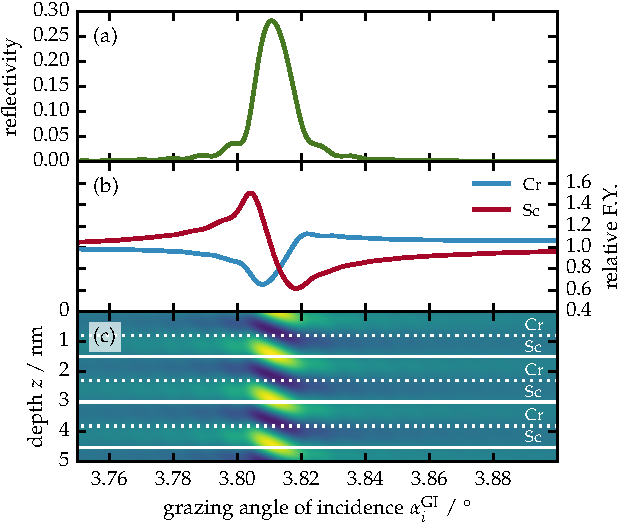
\includegraphics{img/XRF_scheme}
        \caption[X-ray standing wave fluorescence principle.]{%
            Illustration of the grazing incidence X-ray standing wave fluorescence analysis. The exemplary system shown is a bilayer multilayer mirror of Cr and Sc irradiated with a $6.25$ keV photon beam at grazing angles. Changing the grazing angle of incidence $\alpha_i^\text{GI}$ across the first Bragg peak (a) causes a standing wave inside the multilayer (total intensity in first top layers shown in (c)) and cause a relative fluorescence yield for the two different materials as shown in (b). The dotted lines in (a) and (b) indicate the case of interdiffusion and strongly asymmetric interface regions for comparison.}
        \label{ch_theo:fig_xrf_scheme}
\end{figure}

The constructive interference in the Bragg condition, in addition to resulting in a high reflectance, causes the formation of a X-ray standing wave inside the layers. The corresponding intensity distribution in the top first few layer pairs for the example given here is shown in Fig.~\ref{ch_theo:fig_xrf_scheme}(c). The standing wave intensity shifts through the individual layers thereby selectively exciting fluorescence radiation in the respective chemical species while changing the angle of incidence across the Bragg peak. Thus, this yields a method for chemically selective composition analysis with spatial resolution in the sub-nanometer regime called \gls{xsw} analysis. The response curves of the respective relative fluorescence radiation intensity across the Bragg peak for both materials is shown in Fig.~\ref{ch_theo:fig_xrf_scheme}(b). In this example, the fluorescence radiation was calculated according to the discrete sum in Eq.~\eqref{ch_theo:eqn_I_GIXRF_multilayer_discrete} with a sublayer setup as indicated in Fig.~\ref{ch_theo:fig_xrf_multilayer_scheme}(b) and $30$ sublayers per layer pair in each period.

We extended the example above to the case of imperfect layer stacks with interdiffusion and strongly asymmetric interface region thickness. The corresponding calculation is then calculated according to the scheme given in Fig.~\ref{ch_theo:fig_xrf_multilayer_scheme}(c) and is added for comparison to the reflectance and fluorescence yield curves in Fig.~\ref{ch_theo:fig_xrf_scheme}(a) and \ref{ch_theo:fig_xrf_scheme}(b) as dotted lines. The diminished contrast causes a decrease in the peak reflectance of that multilayer system as well as changes in the fluorescence yield.




%     \chapter{Experimental Details and Analytical Toolset} \label{ch_exp}

\section{Synchrotron Radiation}
The radiation emitted by a relativistic charged particle, usually electrons, accelerated to a circular orbit through an external magnetic field is called synchrotron radiation. This radiation is polarized and emitted tangentially to the circular movement of the charged particle in forward direction. In the history of synchrotron radiation, sources have evolved from parasitic use of particle accelerators to the extend of building electron storage rings dedicated for the sole purpose of generating this radiation \cite{munro_chapter_1987}. Its most promitent features are the high brilliance, that is the number of photons per second per unit particle beam cross section and per unit solid angle within $0.1\%$ bandwidth at a specific wavelength, and its huge spectral range of emission. Depending on the energy of the relativistic particles forced on a circular orbit, in modern electron storage rings typically in the order of one to several GeV, the emission covers the range from the terahertz into the hard X-ray regime. The \gls{ptb} operates two laboratories at the dedicated sources, the \gls{bessy} and the \gls{mls} \cite{brandt_metrology_2007}. The two thrid-generation synchrotron radiation sources provide maximum electron energies of $1.7$ GeV (\gls{bessy}) and $0.6$ GeV (\gls{mls}), respectively. Theoretical emission spectra for a single dipole magnet (\emph{bending magnet}) are shown in Fig.~\ref{ch_exp:fig_experimental_synchrotron_spectra} in comparison to black body radiation.
\begin{figure}
 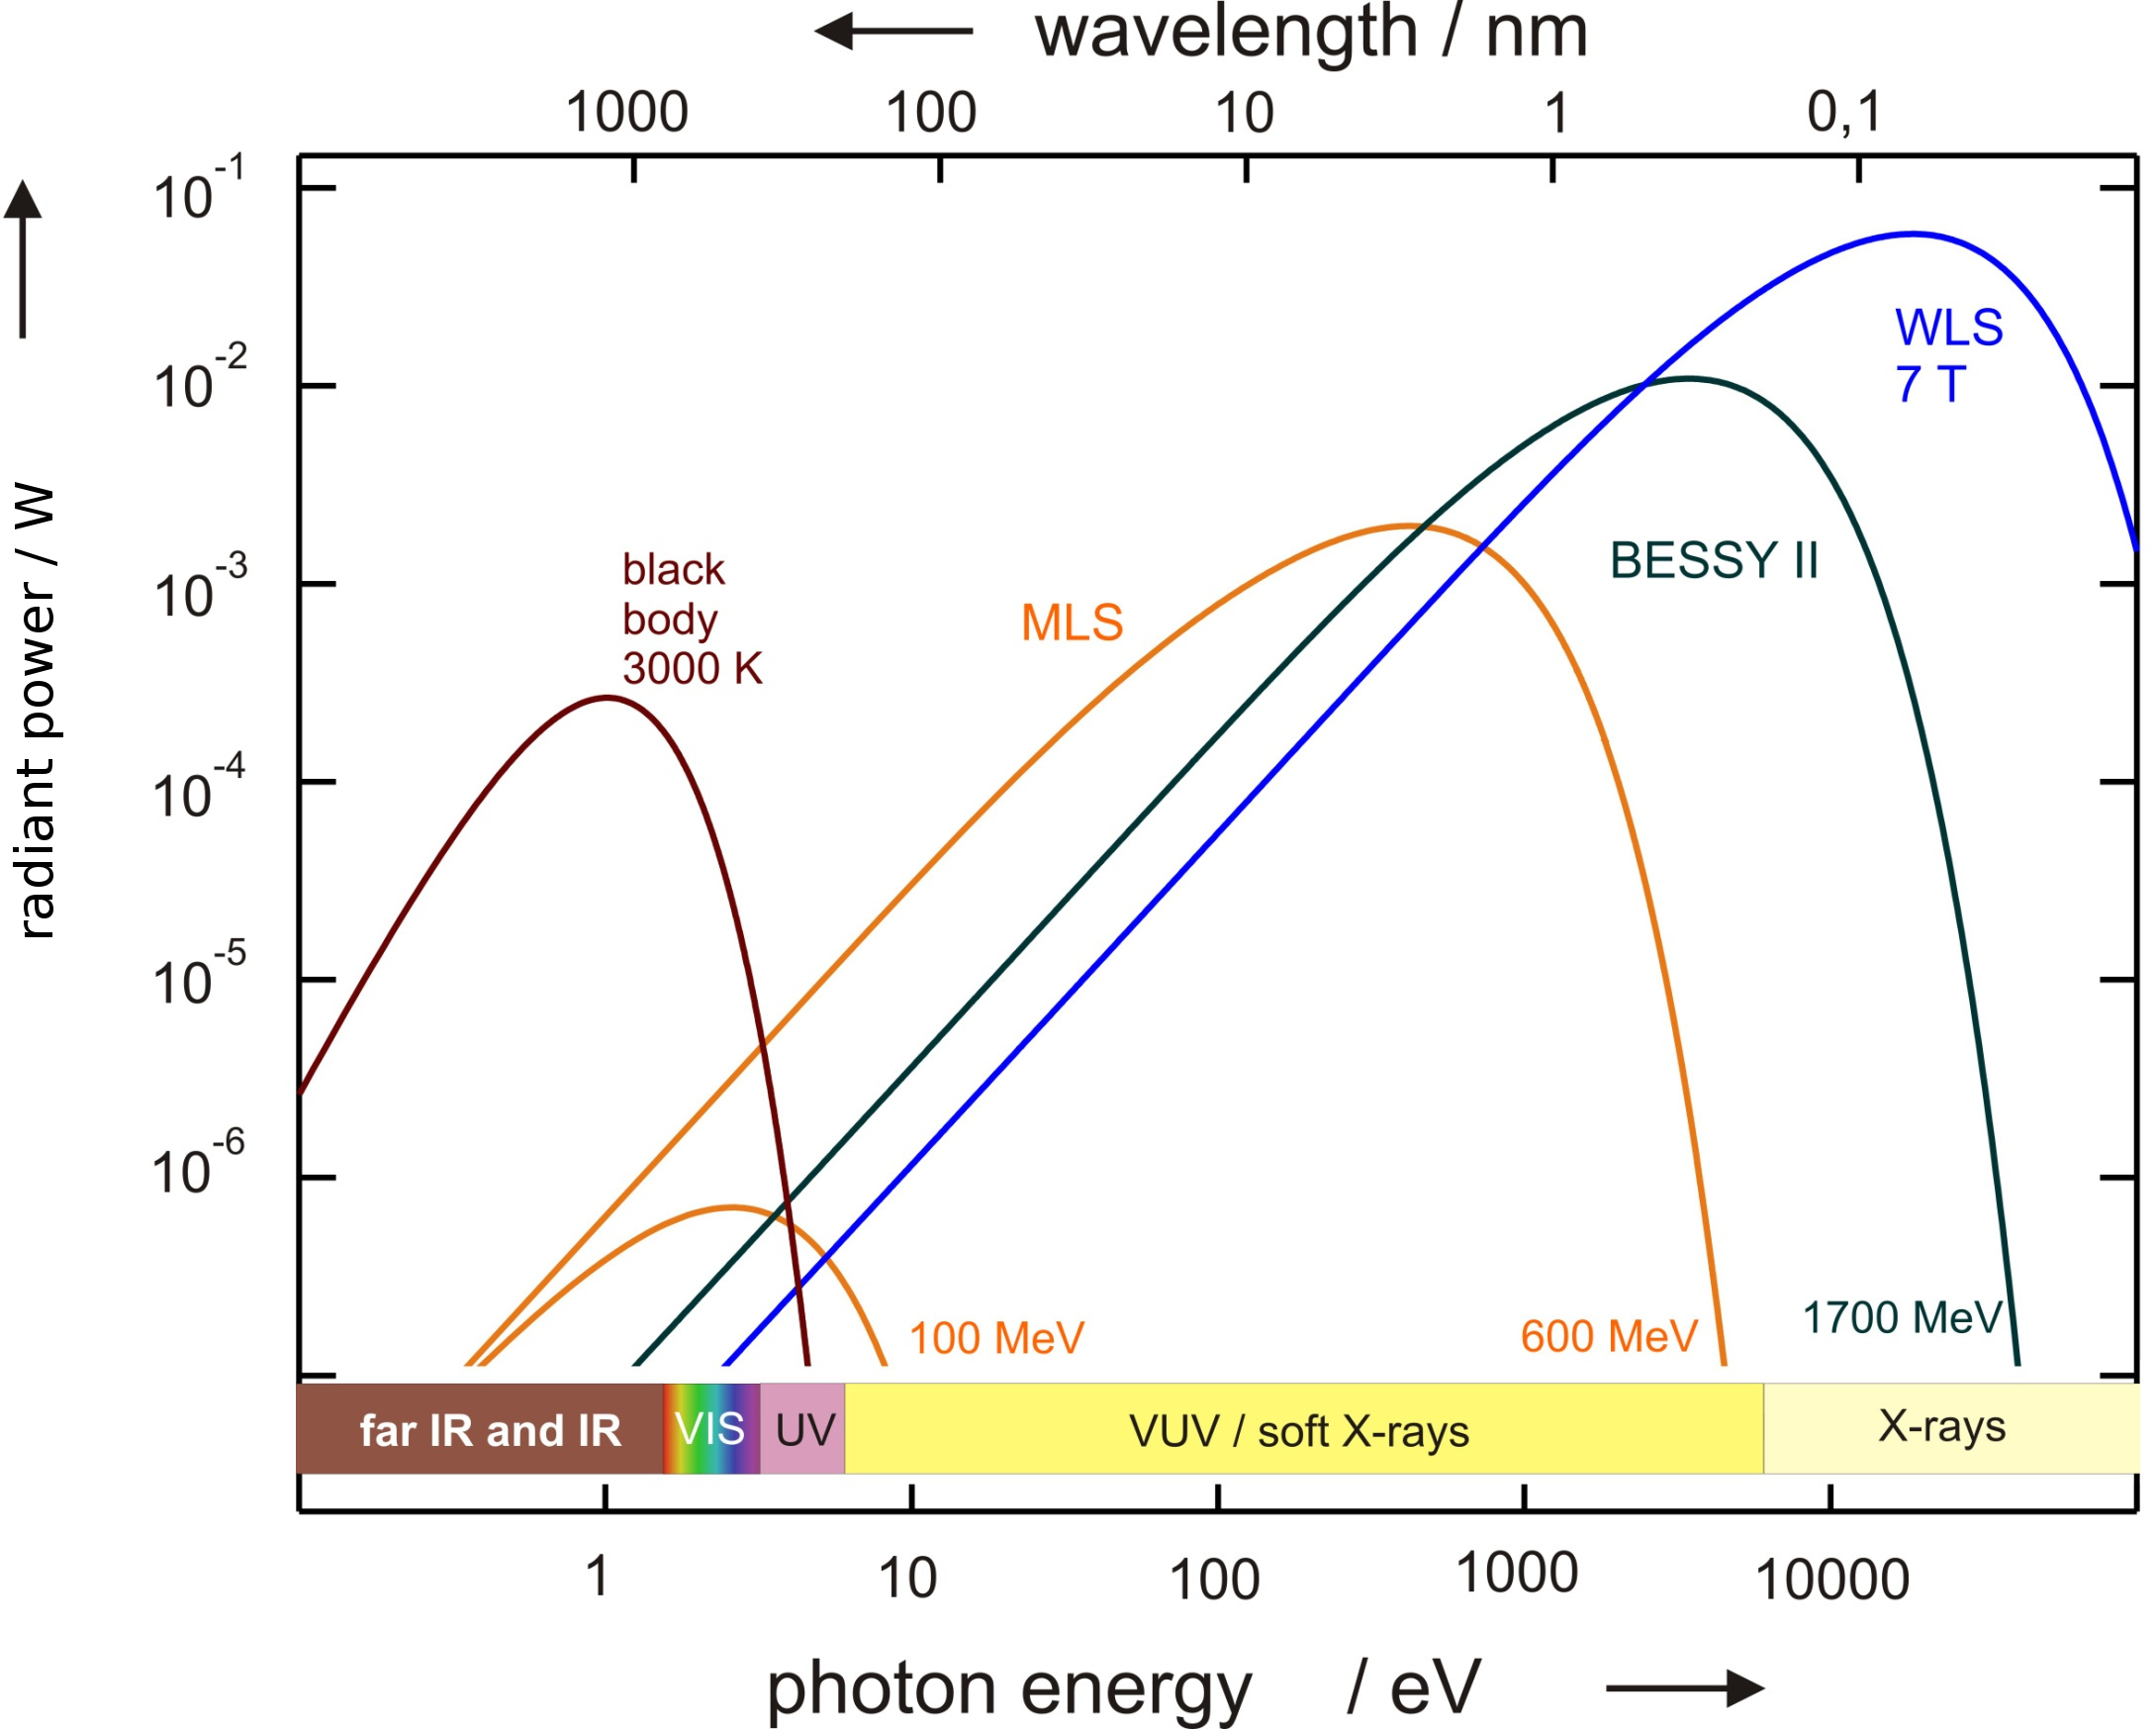
\includegraphics[width=0.7\textwidth]{img/exp-bessy-dipole-spectrum.jpeg}
 \caption[Theoretical synchrotron radiation radiant power spectra]{Theoretical synchrotron radiation radiant power spectra for the \gls{mls} and \gls{bessy} in comparison to black body radiation\footnote{Image taken from \textcite{beckhoff_quarter-century_2009}}. The curves show the radiant power of emission for bending magnets at both electron storage ring facilities for different electron energies. The curve marked WLS shows the radiant power from the $7$ Tesla wavelength shifter insertion device installed at \gls{bessy}.}
 \label{ch_exp:fig_experimental_synchrotron_spectra}
\end{figure}

A very important theoretical aspect of synchrotron radiation, apart from the high brilliance and large spectrum, is the fact that the emission can be calculated exactly from first principles of classical electrodynamics and special relativity. The theory for synchrotron radiation was developed by Schwinger \cite{schwinger_classical_1949} and we shall review its most imporant aspects here. Given all the fundamental and experimental parameters are known, the total emitted radiant power per relativistic particle can be calculated exactly as
\begin{align}
 P = \frac{1}{4 \pi \gls{epsilon_0}} \frac{2}{3} \frac{\gls{e}^2 \gls{c}}{R^2}\Big( \frac{E}{\gls{m_0} \gls{c}^2}\Big)^4 \text{,} \label{ch_exp:schwinger_equation_total_power}
\end{align}
where \gls{e} is the elementary charge, \gls{c} is the speed of light in vacuum, $E$ is the particles energy, \gls{m_0} is the rest mass of the particle and $R$ is the radius of the circular trajectory imposed by the magnetic field. The radiant power is thus inversely proportional to the fourth power of the particles rest mass, which explains the usage of light electrons in comparison with significanlty heavier protons in synchrotron radiation sources. The dependence on the electron energy is visible in another characteristic value for the emitted radiant power, visible as a shift to higher photon energies (smaller wavelengths) in Fig.~\ref{ch_exp:fig_experimental_synchrotron_spectra}, known as the critical energy or critical wavelength \cite{schwinger_classical_1949}, respectively,
\begin{align}
 E_C = \frac{3 \gls{h} \gls{c}}{4 \pi R} \Big( \frac{E}{\gls{m_0} \gls{c}^2}\Big)^3 \text{.} \label{ch_exp:characteristic_energy}
\end{align}
It marks the point in the spectrum, where the integrated radiant power for all values above and below the critical energy are equal \cite{balerna_introduction_2015}. This formula quantifies the shift towards higher energies due to the increase of the electron energy comparing the \gls{mls} and \gls{bessy} emission spectra. Apart from the spectral distribution, the emitted radiation is linearly polarized with an electric field vector oscillating parallel to the plane of the circular orbit. This property, however, is only stricly valid for the emission inside this plane. For radiation above or below, a vertical polarization component (parallel to the surface normal of the orbital plane) exsists. The intensity $I(\lambda,\Psi)$ emitted by a single electron on a circular orbit in direction of the azimuthal angle $\Psi$ at the wavelength $\lambda$ is described by
\begin{align}
  I(\lambda,\Psi) &= \frac{27 \gls{e}^2 \gamma^8 }{36 \pi^3 R^3} \Big(\frac{\lambda_c}{\lambda}\Big)^4 \big(1+ (\gamma \Psi)^2\big)\Big( K_{2/3}^2(\zeta) + \frac{(\gamma \Psi)^2}{1 + (\gamma \Psi)^2} K_{1/3}^2(\zeta)\Big) \text{,}
 \label{ch_exp:schwinger_equation_spectral}
\end{align}
where $\gamma = \sfrac{E}{\gls{m_0} \gls{c}^2}$ and $\Psi$ is the angle between the orbital plane and the observation direction outside of that plane \cite{schwinger_classical_1949}. The characteristic wavelength $\lambda_c = \sfrac{h c}{E_c}$ is given by the critical photon energy defined in Eq.~\eqref{ch_exp:characteristic_energy}. The argument of the modified Bessel funktions of second kind $K_{x}(\zeta)$ is defined as
\begin{align}
 \zeta = \frac{\lambda}{\lambda_c} \big(1 + (\gamma \Psi)^2\big)^\frac{3}{2} \text{.}
\end{align}


The ability to calculate the exact emission and polarization properties of synchrotron radiation based on Eq.~\eqref{ch_exp:schwinger_equation_spectral} with a given electron current and aceptance angle have another very valuable side effect for the field of metrology. It enables the use of synchrotron radiation as a primary standard for electromagnetic radiation within the available spectral range, which is in fact exploited by the \gls{ptb} \cite{thornagel_electron_2001} to provide absolute radiometry.

The dedicated sychrotron radiation facilities, such as \gls{bessy} and the \gls{mls} provide additional possibilities of generating synchrotron radiation beyond a simple bending magnet through different instertion devices. Fig.~\ref{ch_exp:fig_bessy2} gives a shematic overview over the storage ring \gls{bessy}. At each of the marked dipole magnets, synchrotron radiation is produced according the theory presented above. The radiation is transmitted through outlet systems towards a large number of beamlines, which monochromatize and focus the radiation for experimental applications.
\begin{figure*}[htb]
    \def\svgwidth{0.7\textwidth}
    \import{svg/}{bessy.pdf_tex}
    \caption[Schematic overview of BESSY II.]{Schematic overview of the electron storage ring facility \gls{bessy}\footnote{Original image by \gls{hzb}, Ela Strickert, source: \url{https://www.helmholtz-berlin.de/mediathek/bildarchiv/}}. The synchrotron accelerates the electrons coming from the \gls{linac}, which are then injected in the electron storage ring with their full desired energy. Electromagnetic lenses focus and stabilize the beam, as well as deflecting it onto the circular orbit while emitting synchrotron radiation at each dipole (bending) magnet. Cavities reaccelerate the electrons in the storage ring to compensate the energy loss due to the radiation emission.}
    \label{ch_exp:fig_bessy2}
\end{figure*}
Undulators or wigglers are inserted in the straight sections of the \gls{bessy} storage ring with a large number of periodically arranged magnets with alternating polarization forcing the electrons on a sinosoidal beam path. The goal of these insertion devices is to shift the critical energy of the storage ring towards higher energies (wigglers) or to dramatically increase the brilliance within a significantly smaller spectral range compared to bending magnets (undulators). The different effect of the undulators and wigglers on the generated spectrum is determined by the magnetic field strength $B_0$ and the distance between two identical periodic arragnements of the magnets of alternating polarization $\lambda_0$. The deflection parameter quantifies this relation through $K \propto B_0 \lambda_0$. Undulators typically have deflection parameters $K < 1$ while in case of wigglers $K \gg 1$ \cite{munro_chapter_1987}. Technically, the magnetic field strength can be varied by changing the distance (``gap'') between the magnets vertically. By changing the vertical alignment of the magnetic field direction with respect to the beam path, it is even possible to affect the polarization properties of the emitted radiation to obtain circularly or eliptically polarized radiation.
\begin{figure}[htb]
    \def\svgwidth{0.7\textwidth}
    \import{svg/}{mls.pdf_tex}
    \caption[Schematic overview of the MLS]{Schematic overview of the electron storage ring facility \gls{mls}}
    \label{ch_exp:fig_mls}
\end{figure}


The most advanced light source available today, also known as fourth generation source, is following the concept of a \gls{fel} as first invented by \textcite{madey_stimulated_1971}. In that case radiation is produced by a typically single very long undulator inside a linear accelerator instead of a comparatively short straight section of a storage ring. The concept was first demonstrated by \textcite{deacon_first_1977}. \Gls{fel} sources produce highly coherent radiation in the x-ray regime through the principle of \gls{sase} \cite{derbenev_possibility_1982, bonifacio_collective_1984}. Here, the emitted radiation inside the long undulator has a feedback effect on the electron bunch travelling along the beam path. The result is a microbunching of the electron cloud through the electric field of the emitted radiation connected with a (random) wavelength within a certain spectral range defined by the undulator properties. The microbunching causes amplification of that wavelength, which causes an emission spectrum showing several spikes of amplified wavelengths with a noisy background until a saturation level is reached \cite{milton_exponential_2001}.

\section{The Instrumentation for the EUV Spectral Range}
\subsection{The EUV Beamlines at BESSYII and MLS}
The radiation generated in bending magnets or in insertion devices in synchrotron radiation sources typically requires monochromatization and focussing trough a series of optical elements depending on the experimental requirements or designated use cases. In addition, radiation in the \gls{euv} spectral range is absorbed quickly during propagation under atmospheric conditions. It is thus neccessary to maintain a high vacuum from the source points to the experiment and the detector. The two \gls{ptb} beamlines for the \gls{euv} spectral range at the two storage rings \gls{bessy} and \gls{mls} operate on the broad spectrum emitted by bending magnets at each facility. The experiments conducted in the framework of this thesis were performed at both beamlines, exploiting the different radiant power in the required spectral range of the respective experiments. The two beamlines share many technical and design aspects. Thus, the description here will introduce most of these aspects with respect to the SX700 beamline at \gls{bessy}. The differences of the \gls{euvr} at the \gls{mls} will be given below.

\subsubsection{The Soft X-ray Beamline SX700}
The \gls{sx700} at \gls{bessy} provides a monochromatic beam in the spectral range from $\nm{0.7}$ to $\nm{24.8}$ wavelength (corresponding to photon energy range from $\ev{50}$ to $\ev{1800}$) \cite{beckhoff_quarter-century_2009}. The total radiation power and the corresponding relative bandwidth at that beamline are shown in Fig.~\ref{ch_exp:fig_flux_sx700}. The beam size at the entrance aperture to the reflectometer (experimantal end station) is variable through the setting of the exit slits. In the standard setting is approximately \mm{1} by \mm{1} \cite{scholze_high-accuracy_2001} and can be reduced to \mm{0.1} vertical extent (grating dispersion direction) and \mm{0.5} horizontal extent.
\begin{figure}[htb]
    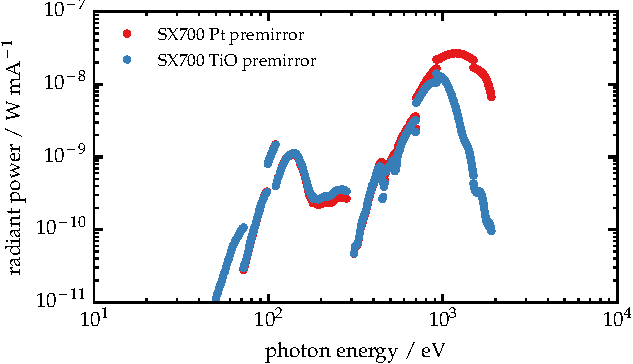
\includegraphics{img/beamline_radiant_power.pdf}
    \caption[Radiant power of the SX700 beamline.]{Radiant power of the SX700 beamline at \gls{bessy} in W per mA storage ring ring current. The two curves differ by the coating on the premirror in the beamline. The TiO coating provides the ability to achieve energies down to \ev{50}, while the Pt coating ensures high radiant power in the high energy range up to \ev{1800}.}
    \label{ch_exp:fig_flux_sx700}
\end{figure}

The monochromatization of the radiation is achieved by a plane grating monochromator with a blazed line grating with 1200 lines per millimeter mounted with its rotational axis within the plane of the storage ring and illuminated perpendicular to the grating lines, yielding the dispersive direction being perpendicular to the storage ring plane. The schematic layout of the beamline is illustrated in Fig.~\ref{ch_exp:fig_sx700_schematic} including the plane grating position of the monochromator, the focussing mirrors and slit positions.
\begin{figure*}[htb]
    \def\svgwidth{\textwidth}
    \import{svg/}{sx700_scheme.pdf_tex}
    \caption[Schematic setup of the SX700 beamline.]{Schematic setup of the \gls{sx700} beamline at \gls{bessy} in top view (upper part) and side view (lower part) \footnote{Original image taken from \textcite{scholze_high-accuracy_2001}}.}
    \label{ch_exp:fig_sx700_schematic}
\end{figure*}
The selection of the desired wavelength at the position of the experimental chamber is done by a horizontal slit at the exit slit. The achievable relative bandwidth depends on the size of this slit as well as on the selected wavelength. It varies between values of $0.5\times 10^{-3}$ and $2.5\times 10^{-3}$ relative bandwidth. As mentioned above, the monochromator grating disperses the incoming broad band radiation into the vertical direction with respect to the storage ring plane. The blaze of the grating ensures high grating efficiency in the first diffraction order, but the selected vertical part of the dispersed radiation still contains parts of higher diffraction orders. This leads to a diminished spectral purity, which reduces the energy resolution. For the purpose of suppression of these higher grating orders, thin metal films in transmission geometry acting as filters are installed close to the entrance aperture to the experimental station supressing radiation energetically above the respective absorption edges of the material.

The \gls{sx700} beamline only has one focussing mirror per horizontal and vertical direction, which differs in position in the beamline and produces different focal points for the two directions. The focussing in horizontal direction (grating dispersion direction) is done trough the toroidal mirror (cf.~Fig.~\ref{ch_exp:fig_sx700_schematic}), which also serves as a collector mirror for both axis and parallizes the beam in vertical direction. The focal point is located in the exit slit to ensure high energy resolution. The vertical focussing is done by an additional focussing mirror after the monochromator grating with a focal point about \m{2} behind the exit slit in propagation direction. Due to the large distance of the two focussing elements to the experimental station, a low divergence of the beam of about $1.6$ mrad $\times$ $0.4$ mrad is achieved.

\subsubsection{The Extreme Ultraviolet Beamline EUVR}
The general layout and operation principle of the \gls{euvr} beamline is identical to that of the \gls{sx700} beamline described in the previous paragraph with some differences in the focussing, which are described in the following. Due to the lower electron energy in the \gls{mls} storage ring, the spectrum of both beamlines differs with a spectral range shifted to longer wavelengths in the \gls{euvr} beamline with respect to the \gls{sx700} beamline. The wavelength range covered by the \gls{euvr} beamline is between \nm{5} to \nm{50} (corresponding to photon energies from approximately \ev{25} to \ev{248}). In contrast to the \gls{sx700} beamline, the foci for horizontal and vertical direction are both at the position of the exit slit with an additional refocussing mirror behind that slit. This increases the divergence of the beam to approximately $4$ mrad in both directions, but together with the shifted bending magnet spectrum of the \gls{mls} allows higher photon flux through the larger aperture of the torodial mirror. The main properties of both beamlines and their differences are given in Table~\ref{ch_exp:tbl_beamline_properties}. The optics of both beamlines in comparison are shown in Fig.~\ref{ch_exp:beamline_optics}.
\begin{table*}
\centering
\begin{tabular}{lrr}
\toprule
Parameter 			& \gls{sx700} 		& \gls{euvr}\\ \midrule
Wavelength range 		& $\nm{0.7}$ to $\nm{24.8}$ 	& $\nm{5}$ to $\nm{50}$\\
Spot size (standard settings)			& $\mm{1} \times \mm{1}$ 		& $\mm{0.1} \times \mm{0.1}$ to\\ 
&&$\mm{2} \times \mm{2}$\\
Beam divergence			& $\mrad{1.6}\times \mrad{0.4}$ 	& $\mrad{4}\times \mrad{4}$\\
Linear polarization (horizontal)	& $\SI{98}{\percent}$ 		& $\SI{40}{\percent}$ to $\SI{98}{\percent}$\\
 \bottomrule
\end{tabular}
\caption{Beamline parameters of the two EUV beamlines \gls{euvr} and {sx700} in comparison.}
\label{ch_exp:tbl_beamline_properties}
\end{table*}
\begin{figure*}[htb]
    \def\svgwidth{\textwidth}
    \import{svg/}{beamline_optics.pdf_tex}
    \caption[Schematic optics of the SX700 and EUVR beamlines.]{Schematic optics of the SX700 and EUVR beamlines. The \gls{sx700} beamline has a small beam divergence due to the single focussing in both horizontal and vertical direction. The focal point positions differ by approximately \m{2}. The \gls{euvr} beamline offers significanly higher photon flux due to the larger collector mirror aperture in conjuction with the bending magnet spectrum at the \gls{mls}. The beam spot sizes are variable and can be significanlty smaller in comparison to the \gls{sx700} beamline at the position of the experiment due to refocussing.}
    \label{ch_exp:beamline_optics}
\end{figure*}

\subsection{The Experimental Endstations at the EUVR and SX700 Beamlines}
All experimenents in the \gls{euv} spectral range within the framework of this thesis were conducted at the beamlines \acrshort{euvr} and \acrshort{sx700}. Each of the beamlines is equipped with an experimental end station containing the detectors, mounts for \gls{ccd} cameras and a goniometer to adjust the angle of the sample holder with respect to the beam. Due to the high absorption of the \gls{euv} radiation in air, both chambers need to be kept under high vacuum conditions, typically below the limit of \mbar{3E-6}.

The end stations differ in the size and weight of samples, which can be mounted on the sample holder. The large reflectometer at the \gls{euvr} beamline was designed with heavy and large samples in mind, whereas the ellipso-scatterometer at the \gls{sx700} beamline covers a larger anglular range for both the detector and the sample holder. In the following the two different setups with their primary features are summarized. 

\subsubsection{The large reflectometer at the \gls{euvr} beamline}
The large reflectometer serving as the end station at the \gls{euvr} beamline was designed for reflectometry and scatterometry measurements for samples with a weight of up to \SI{50}{\kg} and a maximum diameter of \mm{550} in mind\cite{tummler_characterization_2003}. The available axis of movement and rotation are shown in Fig.~\ref{ch_exp:fig_bigref}.
\begin{figure*}[htb]
    \def\svgwidth{\textwidth}
    \import{svg/}{bigref.pdf_tex}
    \caption[The BigRef.]{The large reflectometer and end station of the \gls{euvr} beamline at the \gls{mls}. A photograph of the internal mechanics and the vacuum chamber is shown in (a). The schematic layout of the goniometer axes and the detector arm are shown in (b).}
    \label{ch_exp:fig_bigref}
\end{figure*}
The sample holder plate allows for linear movement in all three orthogonal directions as well as angular rotations in three axis. The latter allows to measure samples, e.g.~samples with an anisotropy, with radiation impinging from all directions, if the sample is mounted in the center position of the sample holder. The rotation around the $\Theta$-axis covers the range from $\SI{-30}{\degree}$ to $\SI{95}{\degree}$ relative to the incoming beam. Thus, enabling reflectometry and scatterometry  normal incidence to grazing incidence angles together with the detector arm rotation around the $2\Theta$-axis from $\SI{-5}{\degree}$ to $\SI{190}{\degree}$. The distance of the detector to the sample is variable through the \emph{Det-R} axis from a minimum value of $\mm{150}$ to $\mm{550}$.

The detector mount is equipped with up to $4$ diodes, which can be rotated to face either the sample or the incoming beam. The diodes used within the framework of this thesis are $\mm{4.5} \times \mm{4.5}$ and, optionally $\mm{10} \times \mm{10}$, GaAsP photodiodes. The detector holder can be moved along the $\Theta$ and $2\Theta$ rotational axes, labeled as \emph{Det-X} direction in Fig.~\ref{ch_exp:fig_bigref}, which allows to take measurements in the \emph{out-of-plane}\footnote{The out-of-plane scattering direction refers to radiation scattered outside of the scattering plane spanned by the surface normal of the sample and the impinging beam direction.} direction in s-polarization.

\subsubsection{The Ellipso-scatterometer at the \gls{sx700} beamline}
The ellipso-scatterometer is a reflectometer similar to the large reflectometer providing the end station for the \gls{sx700} beamline. Its capabilities differ from the large reflectometer by a wider reachable angular range for both the detector movement as well as the sample movement. The angular and linear movements and axes are shown in Fig.~\ref{ch_exp:fig_elli} together with a photograph of the goniometer and detector arm.
\begin{figure*}[htb]
    \def\svgwidth{\textwidth}
    \import{svg/}{elli.pdf_tex}
    \caption[The EUV ellipso-scatterometer.]{The EUV ellipso-scatterometer and end station at the \gls{sx700} beamline at \gls{bessy}. The internal mechanics of the goniometer and the detector arm are shown in (a). The schematic layout of the axes an the movable detector arm are given in (b).}
    \label{ch_exp:fig_elli}
\end{figure*}
In contrast to the large end station at the \gls{euvr} beamline, it can hold samples with a size of approximately $\mm{13.5} \times \mm{13.5}$ and a maximum of \SI{5}{\kg} in weight. However, the rotational movement of both the detector and the sample holder allow for a larger angular range. In consequence, measurements in s-polarization and well as p-polarization can be conducted on the same sample. With the capability to mount a polarization analyzed at the detector holder, polarization resolved measurements are thus possible \cite{soltwisch_polarization_2015}.

\section{Grazing-incidence X-ray Fluorescence at the FCM Beamline} \label{ch_exp:sec_xrf_at_fcm}
The \gls{gixrf} measurements of the Cr/Sc sample systems were performed at the \gls{fcm} bending magnet beamline \cite{krumrey_design_1998} in the \gls{bessy} laboratory. The necessary photon energies to excite the K-edge x-ray fluorescence of chromium and scandium, are well above the spectral range of the \gls{euvr} and \gls{sx700} beamlines in the order of several \si{\kilo\electronvolt}. The general setup and design of the \gls{fcm} beamline is very similar to that of the \gls{sx700} beamline, with the exception of the four crystal monochromator, which replaces the plane grating monochromator in the x-ray spectral range. It offers tunable photon energies from \kev{1.75} to \kev{10.0}. A high energy resolution of $E/\Delta E = 10^4$ is attained by the convolution of four exchangeable crystal Bragg reflections. The monochromator can be equipped with two monochromator crystals. For the high energy range above approximately \kev{3.5} to \kev{10.0} silicon is used. In the lower energy range between \kev{1.75} and \kev{3.5} higher radiant power is available through the usage of a InSb crystal. A schematic overview of the \gls{fcm} beamline can be found in Fig.~\ref{ch_exp:fig_fcm_scheme}.
\begin{figure}[htb]
        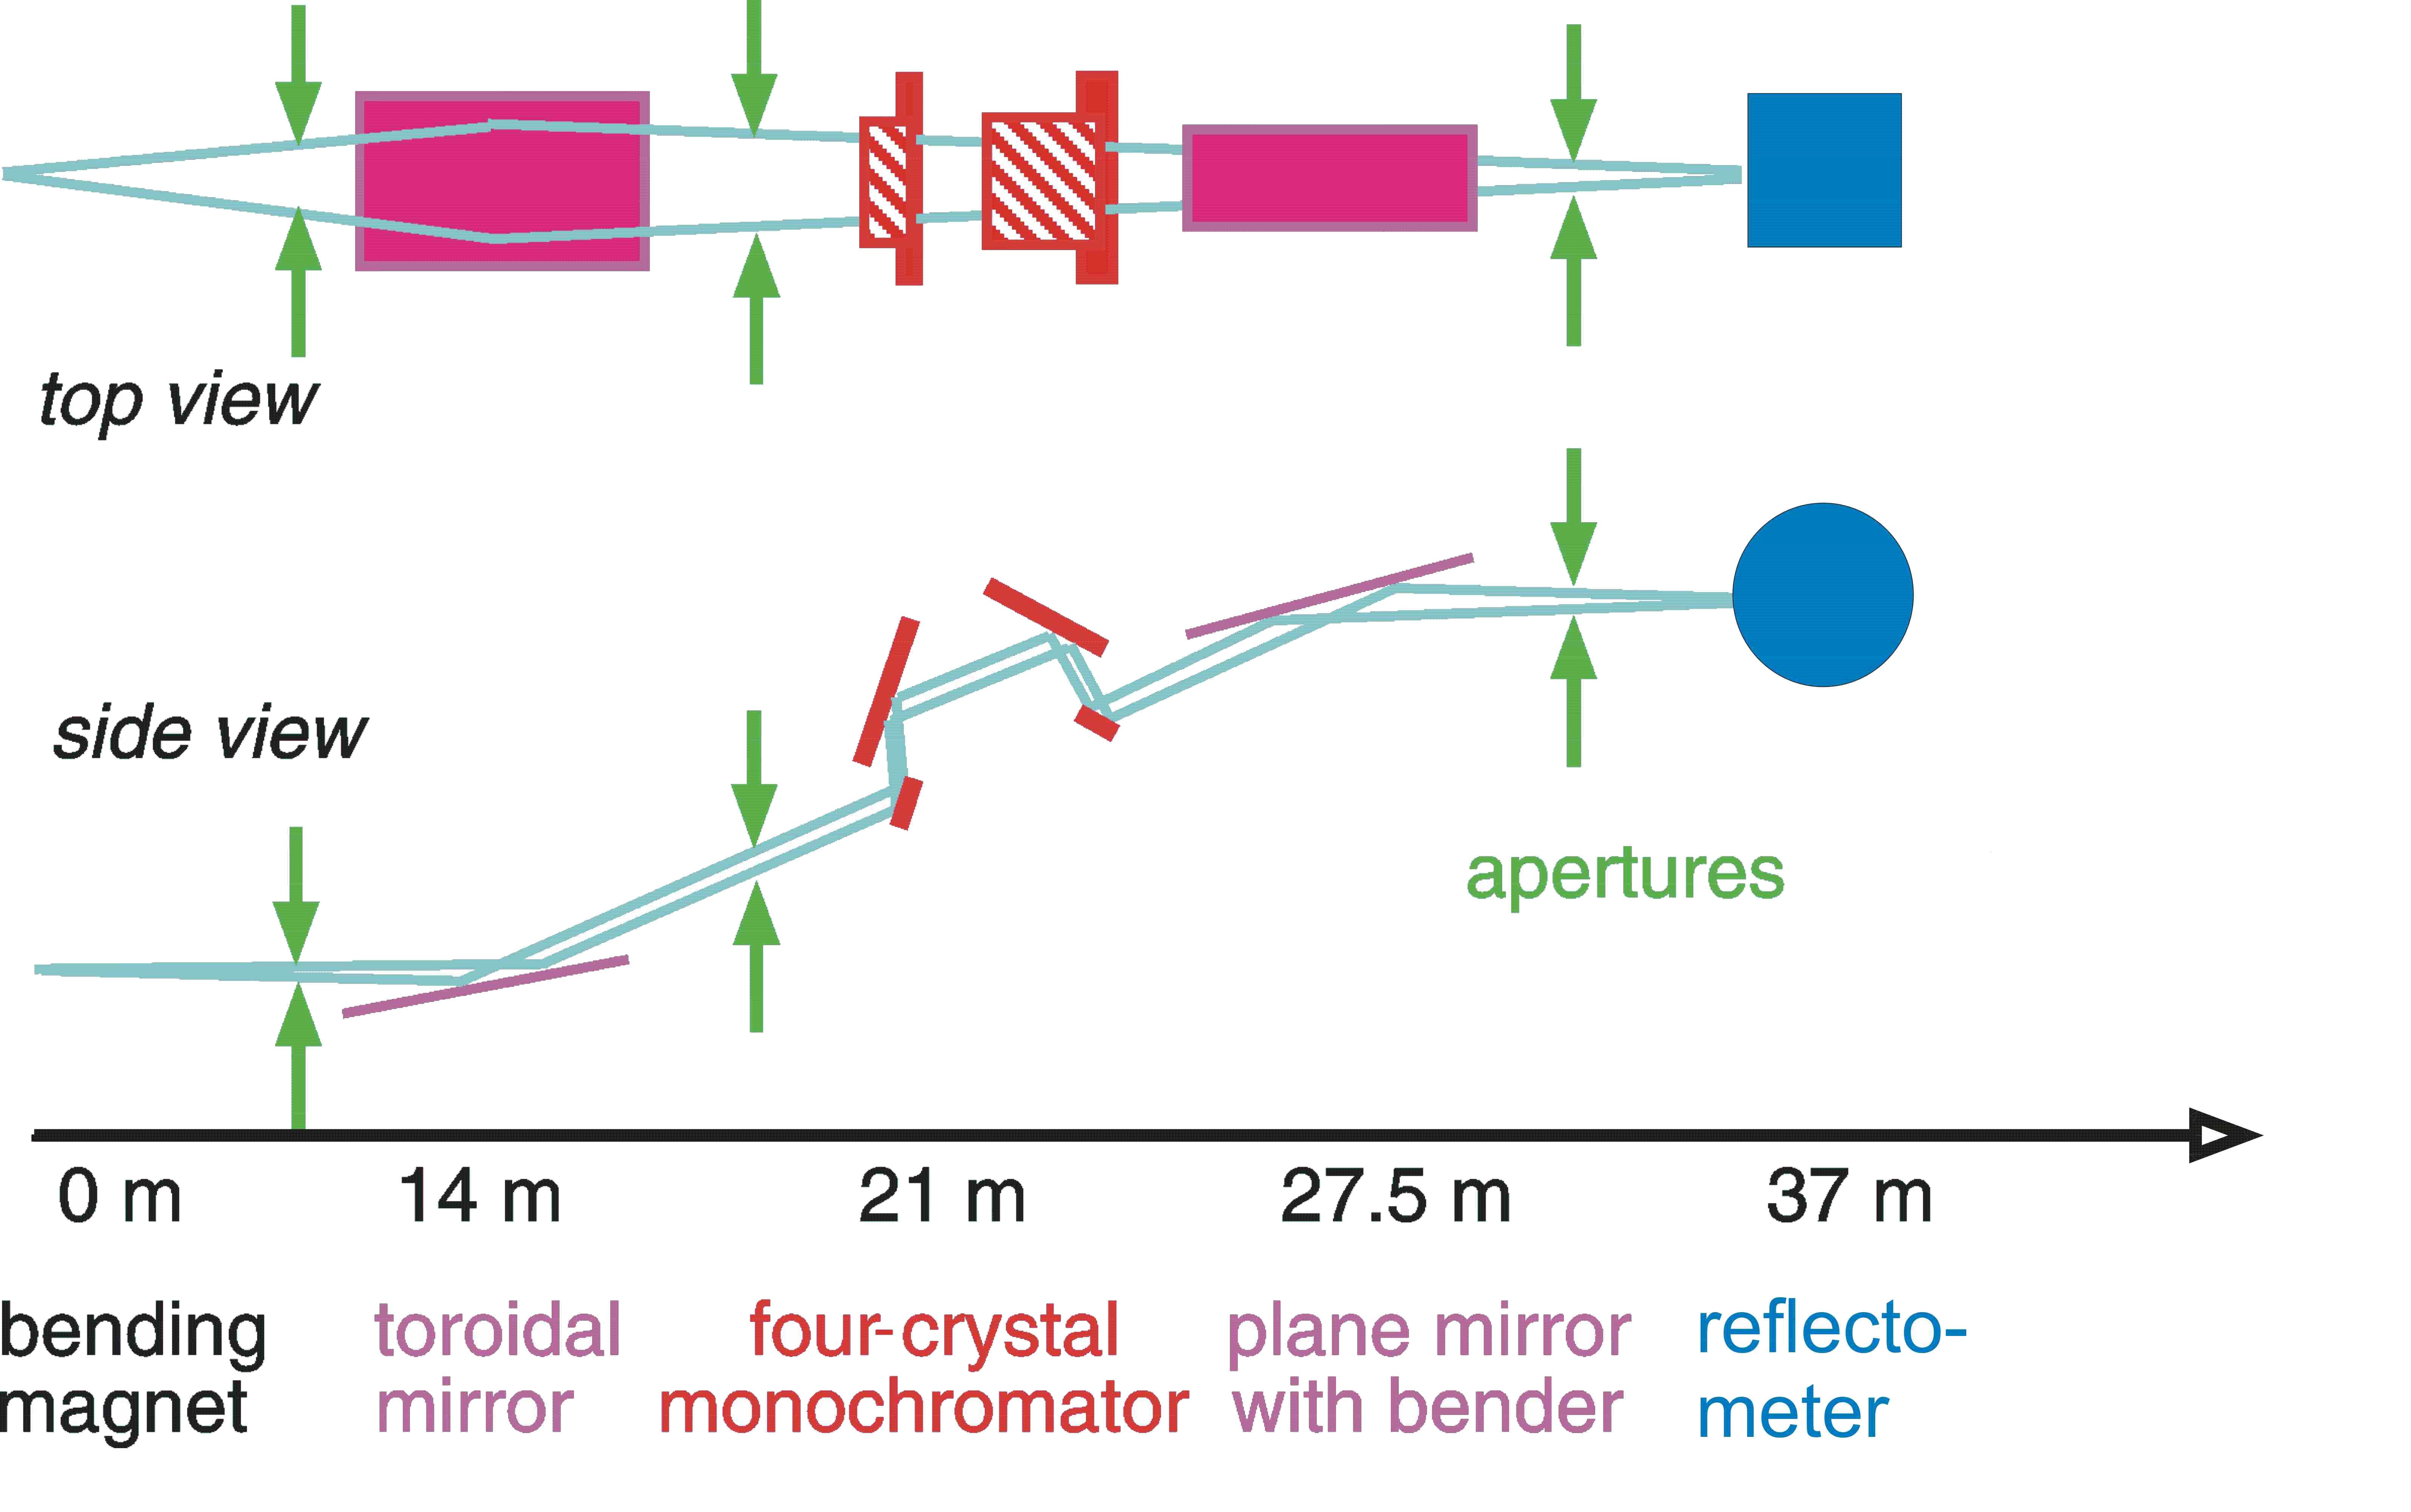
\includegraphics[width=0.7\textwidth]{img/FCMScheme.png}
        \caption[FCM beamline scheme.]{%
            Schematic layout\footnote{Original image taken from \textcite{krumrey_design_1998}.} and optical path of the \gls{fcm} beamline at \gls{bessy}. The setup is comparable to the \gls{sx700} beamline, but uses a four-crystal monochromator setup instead.}
        \label{ch_exp:fig_fcm_scheme}
\end{figure}

The end station used for the \gls{gixrf} experiments is a specialized chamber for \gls{gixrf}, \gls{txrf} and \gls{xrr} \cite{lubeck_novel_2013} depicted in Fig.~\ref{ch_exp:fig_gixrf_chamber}. It is equipped with a detector arm and a sample goniometer allowing to measure grazing incidence angles of \SI{0}{\degree} to \SI{60}{\degree}. The detector arm holds a diode allowing \gls{xrr} measurements. Perpendicular to the beam direction, an energy dispersive \gls{ssd} is mounted close to the sample surface. It allows to detect fluorescence radiation emitted from the sample energetically resolved. The samples can be rotated with respect to the storage ring plane in order to allow a variable polarization impinging on the surface.



\begin{figure*}[htb]
    \def\svgwidth{\textwidth}
    \import{svg/}{gixrf_chamber.pdf_tex}
    \caption[The GIXRF chamber.]{The schematic layout of the dedicated \gls{gixrf} chamber\footnote{Images taken from \textcite{lubeck_novel_2013}.}. This end station can be mounted to the \gls{fcm} or \gls{pgm} beamlines to conduct grazing-incidence \gls{xrf} experiments. In (a), the schematic exterior layout and, in (b), the interior layouts are shown.}
    \label{ch_exp:fig_gixrf_chamber}
\end{figure*}

\section{Sample systems}
The samples studied in the framework of this thesis are designed to work as near-normal incidence mirrors for the \gls{euv} spectral range. The underlying principle of an artificial one dimensional Bragg crystal requires the deposition of thin layered systems with high periodicity and stability. The experiments presented here were conducted on two sets of sample types as prototypes of mirrors for two different spectral ranges. The theoretical description of the principle of multilayer mirrors in Sec.~\ref{ch_theo:sec_multilayer} of Ch.~\ref{ch_theo}, optical contrast, i.e.~a large as possible difference in the real part of the refractive index $n$, is required to achieve large reflectivities while maintaining a low absorption.



\subsection{Choice of the Chemical Species and Multilayer Design}
\label{ch_exp:sec_multilayer_design}
This thesis investigates systems designed to reflect radiation in two spectral ranges, the \emph{water window} with wavelengths from \nm{2.2} to \nm{4.4} and the range from \nm{12.4} to \nm{14.0} with a wide range of applications, e.g.~for the next-generation lithography. The choice of the chemical species for the multilayer systems, apart from trivial properties such as non-toxicity and solidity, is largely influenced by the electronic structure of the respective materials, since large changes in the refractive index, i.e.~large optical contrast with respect to a second material, can be expected close to resonances in the electronic structure. The demand for low absorption also requires species, where the absorption edges are energetically higher or far lower than the desired spectral range of operation. For a well defined interface it is also neccessary that the two materials are mostly inert and do not react with one another. The latter would potentially lead to inevitable intermixing and thus a loss of a sharply defined interface.

\paragraph{Cr/Sc multilayer system}
In case of the water window spectral range, we investigated samples designed for a peak reflectance at a wavelength closely above \nm{3.14}, where the L3 edge of scandium (Sc) is found. Fig.~\ref{ch_exp:fig_crsc_contrast} shows the refractive index of Sc and the second material chromium (Cr) in the water window spectral range. 
\begin{figure}[htb]
        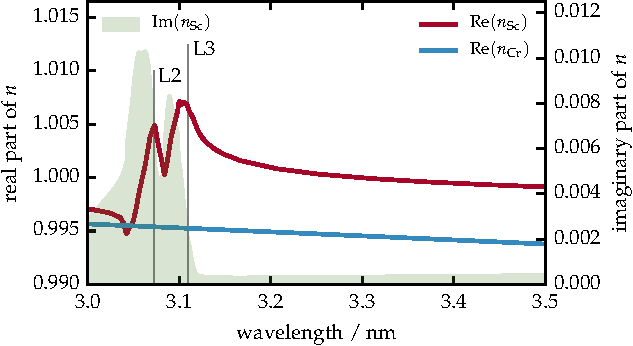
\includegraphics{img/Cr_Sc_contrast}
        \caption[Refractive indices of Cr and Sc in the water window.]{%
            Refractive indices of Cr and Sc with the water window spectral range. The marked absorption edges are the L2 and L3 edge of Sc. The imaginary part of the refractive index accounts for the absorption and is shown for Sc. Above the L3 edge is the highest contrast for the two materials providing the highest potential reflectivity in a periodic multilayer arrangement.}
        \label{ch_exp:fig_crsc_contrast}
\end{figure}
The periodic multilayer of the systems investigated here, were therefore binary alternating layers of Cr and Sc. The required nominal period thickness $D$, i.e.~the thickness each periodically repeated layer stack, for the design goal of a peak reflectivity at $\lambda=\nm{3.14}$ is $D=\nm{1.573}$ with a layer thickness ratio of $\Gamma=0.5$ of both materials. To protect the Sc layers from oxidation, an additional capping layer Cr of approximately $d_\text{cap} = \nm{3}$ was added as the surface layer. The binary layer stack was repeated $N=400$ times per bilayer.

The Cr/Sc multilayer sample was prepared at the DESY X-ray multilayer 
laboratory by DC magnetron sputtering. The deposition was performed at $0.133$ 
Pa ultrahigh purity Ar ($99.999\%$) and a power of $200$ W for both Sc and Cr 
sputtering targets. The multilayer is composed of alternating layers of Cr and 
Sc with periodic replication of the bilayer stack by $N=400$ times. The 
substrate is a superpolished Si wafer piece. The sample dimensions measure 
approximately $(20 \times 20)$ mm$^2$. More details can be found elsewhere 
\cite{prasciolu_thermal_2014}. The multilayer mirror was designed to reflect 
radiation in the water window energetically, just below the Sc L edge, close to 
a $3.1$ nm wavelength at an angle of incidence (AOI) of $\alpha_i = 
\SI{1.5}{\degree}$.


\paragraph{Mo/Si multilayer systems}
The second set of systems under investigation in this thesis is composed out of $50$ to $65$ bilayers Molymdenum (Mo) and Silicon (Si). Both materials show a very low absorption in the range from \nm{12.4} to \nm{14.0}, with the Si L2 edge forming the lower wavelength limit for the usage as a mirror system in this combination. The respective refractive indices are given in Fig.~\ref{ch_exp:fig_mosi_contrast}.
\begin{figure}[htb]
        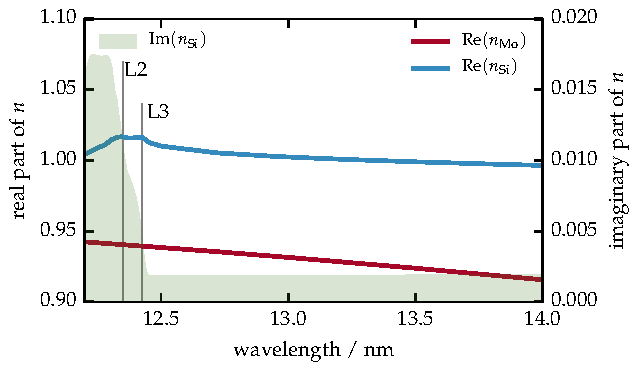
\includegraphics{img/Mo_Si_contrast}
        \caption[Refractive indices of Mo and Si in the wavelength range from \nm{12.4} to \nm{14.0}.]{%
            Refractive indices of Mo and Si in the wavelength range from \nm{12.4} to \nm{14.0}. The L2 absorption edge of Si marks the lower wavelength limit for the applicability of this material combination in multilayer mirror systems.}
        \label{ch_exp:fig_mosi_contrast}
\end{figure}

Finally, the sample systems can contain additional materials, which serve as barrier layers. The two species used for our samples are Boroncarbite (B$_4$C) and Carbon (C). Those two materials do not have any absorption edges in the given relevant spectral range and additionally show low contrast to the respective spacer materials Si and Cr. The details of the respective sample layouts are discussed in the respective sections of the following chapters.

\subsection{Multilayer Deposition by Magnetron Sputtering} \label{ch_exp:sec_magnetron_sputtering}
The multilayer samples investigated here were fabricated by the DC magnetron sputtering technique \cite{stearns_fabrication_1991} by two different multilayer and optics groups. The Mo/Si multilayer samples were fabricated by Stefan Braun at the Fraunhofer IWS, Dresden, Germany and the Cr/Sc samples are by Sa\v{s}a Bajt from the Optics Group at CFEL, DESY, Hamburg in Germany.

Magnetron sputtering is a physical vapor deposition technique. A vacuum chamber is equipped with a substrate to be coated, in our case silicon, and one or more sputter targets. Depending on the intended design of the multilayer to be deposited, those targets are the respective materials, which later form the individual layers. In the DC magnetron sputtering system, a strong electric field is applied between the substrate and the sputter targets. The vacuum chamber containing those parts is then filled with a sputter gas, typically ultrapure Ar gas (\SI{99.999}{\percent}), with partial pressures in the range from \mbar{E-3} to \mbar{E-2} \cite{stearns_fabrication_1991}. The strong electric field ionizes the sputter gas causing the ions to be accelerated towards the sputter targets (cathode) and form a charged plasma. Upon impact in the target, atoms and electrons of the condensed matter phase of the respective material are released and travel towards the substrate. The released atoms condense there, forming bonds and creating a slowly growing layer. The thickness of the layer can be fine tuned through the deposition time. The additionally released electrons, while being accelerated towards the substrate (anode), collide with the sputter gas atoms and cause further ionization. In order to avoid damage of the forming layer at the substrate, strong magnetic fields are applied to the sputter targets. This confines the movement of the charged particles (the plasma) sputter gas ions and electrons to the region close to the target surface. Thereby, increasing the collision (ionization) probability of electrons and the gas atoms through the helical movement in the magnetic field while keeping those particles away from the substrate. To ensure homogeneous layer deposition, the substrate is kept under permanent rotation. A schematic DC magnetron sputtering system is depicted in Fig.~\ref{ch_exp:magnetron_sputtering_schematic}.
\begin{figure}[htb]
        \def\svgwidth{0.65\textwidth}
	\import{svg/}{magnetron.pdf_tex}
        \caption[Schematic setup of a magnetron sputtering deposition system.]{%
            Schematic setup of a magnetron sputtering deposition system\footnote{Original image taken from \textcite{stearns_fabrication_1991}}.}
        \label{ch_exp:magnetron_sputtering_schematic}
\end{figure}


For both samples, silicon serves as the substrates for the deposition process. The surfaces are super polished with mechanical polishing methods to reduce any prior surface roughness. The sample size and shape differ for the systems investigated. In case of the Mo/Si mirror samples, wafer pieces of approximately $\mm{20} \times \mm{20}$ (photograph shown in Fig.~\ref{ch_exp:fig_mosi_sample}) and round substrates with approximately \mm{20} in diameter were used.
\begin{figure}[htb]
        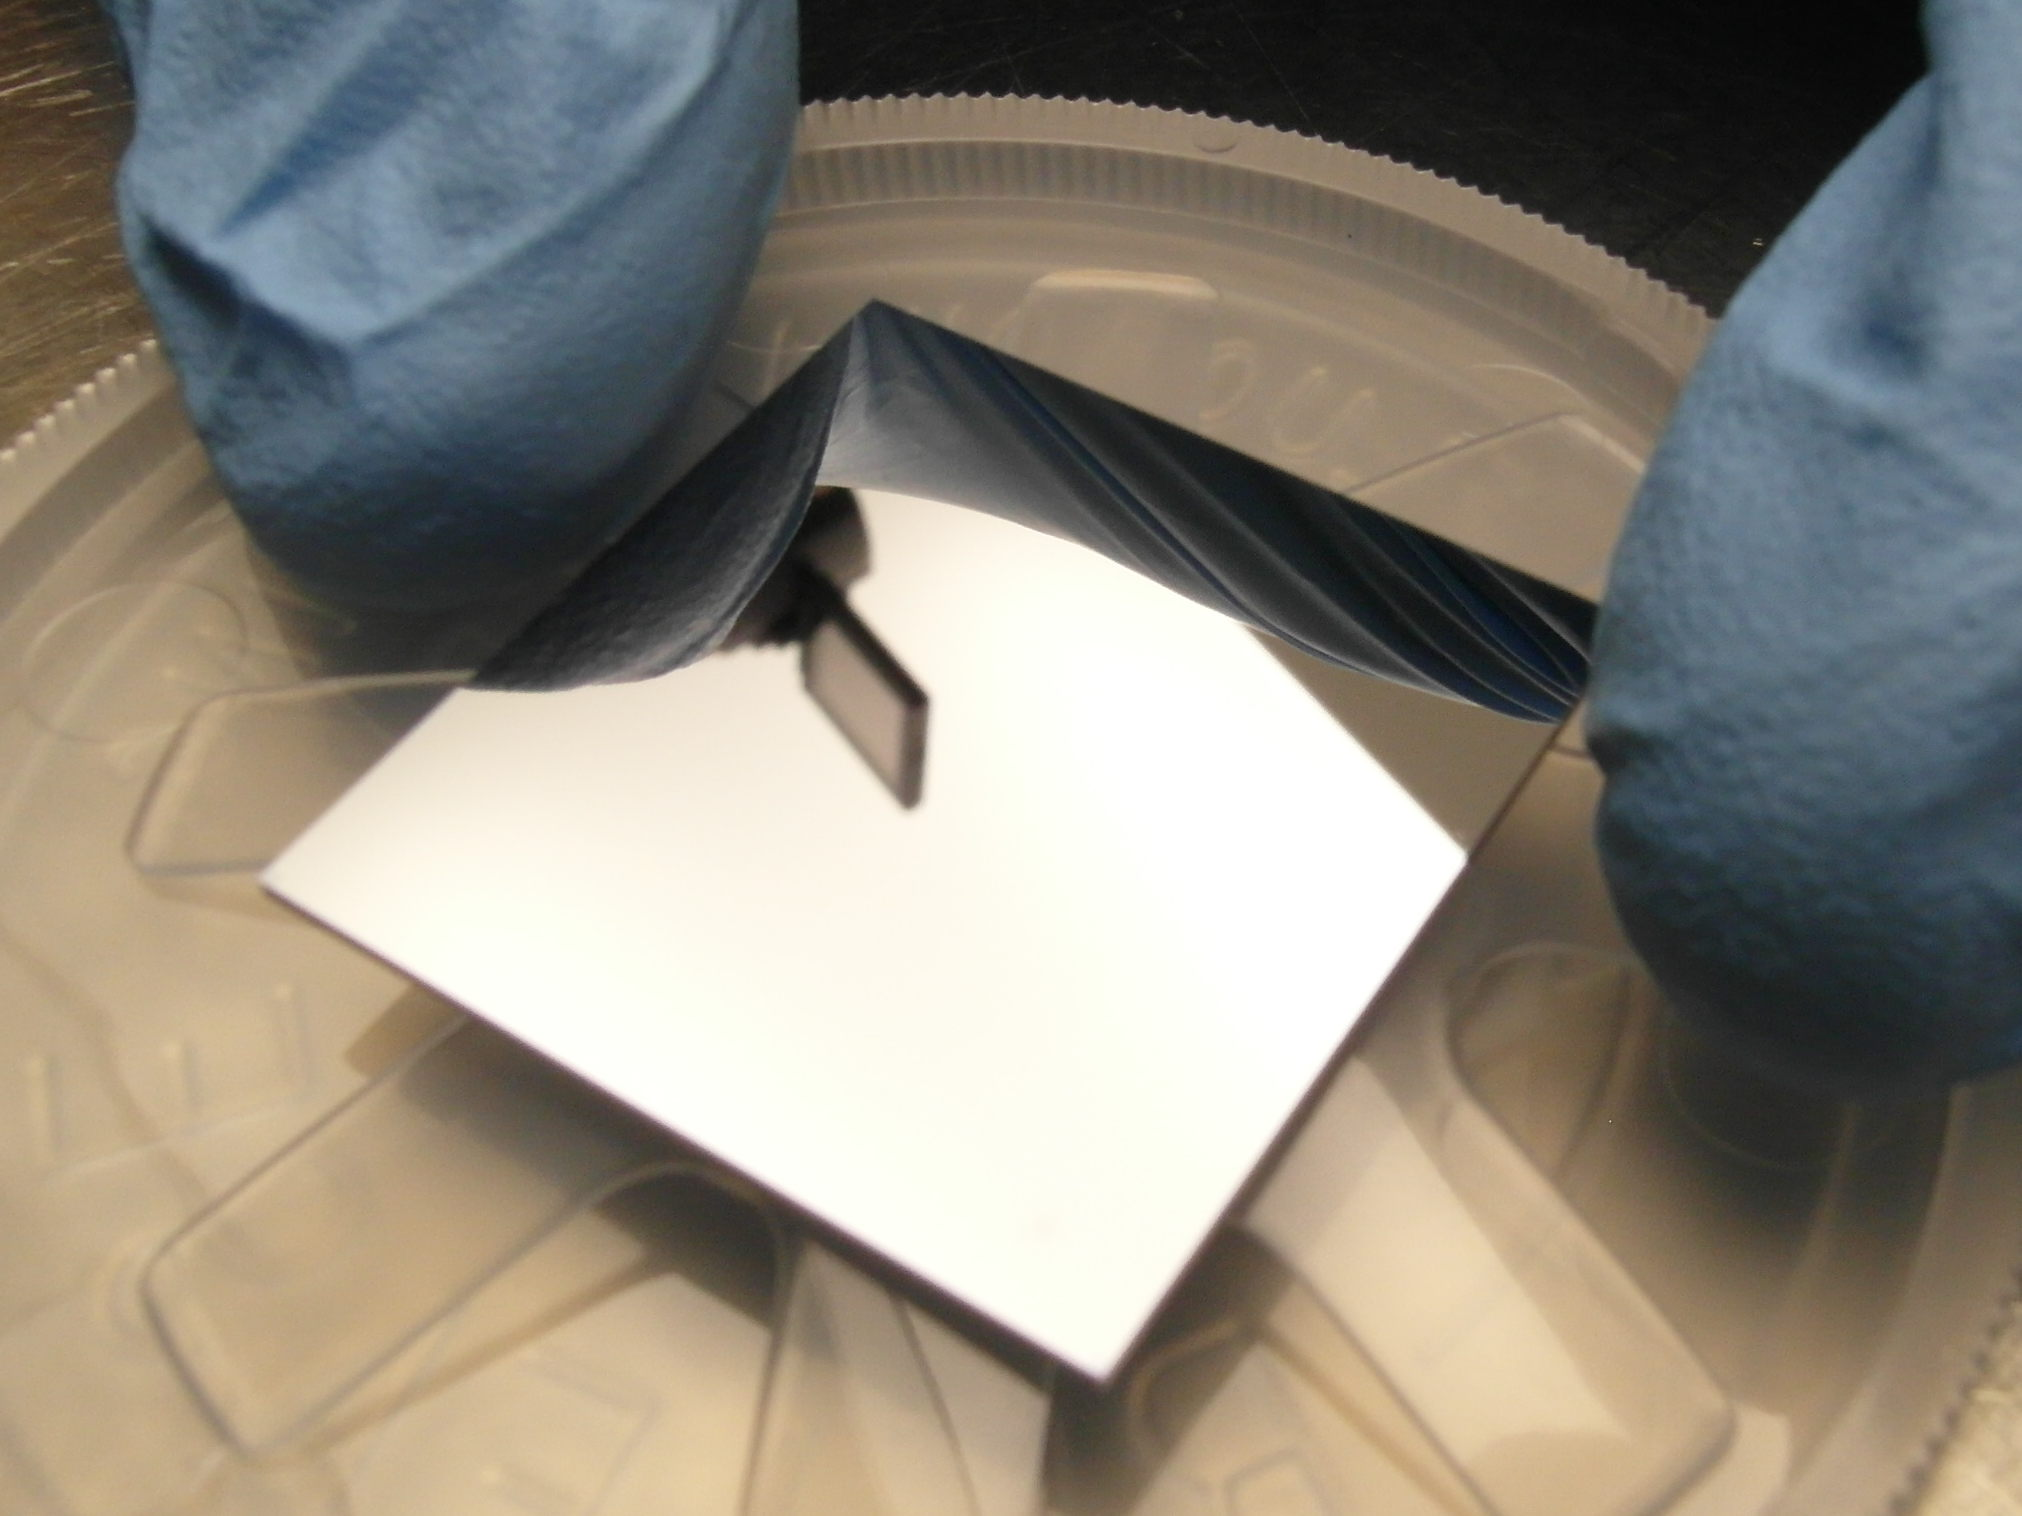
\includegraphics[width=0.4\textwidth]{img/SAM_1910_v1}
        \caption[Mo/Si multilayer sample.]{%
            Photograph of a Mo/Si multilayer mirror sample with dimensions of $\mm{20} \times \mm{20}$.}
        \label{ch_exp:fig_mosi_sample}
\end{figure}
In case of the Cr/Sc systems, wafer pieces of varying size but approximately $\mm{10} \times \mm{20}$ served as the substrate.

\section{Analytical Tools}
In this thesis, several experiments are conducted on different sample systems requiring a dedicated analytical toolset to analyze the sets of data and implement the theoretical calculations based on the models introduced in chapter~\ref{ch_theo}. For that purpose, dedicated software was developed to enable the quantitative analysis conduced in the following chapters. Here, an overview of the software packages and their relation to those already existing and integrated into the framework is given.

All software was written in the \emph{Python} programming language using the \emph{Numpy} and \emph{Scipy} frameworks \cite{walt_numpy_2011} for data analysis and scientific computing. The graphical representation of the data and calculations was done using the \emph{Matplotlib} \cite{hunter_matplotlib:_2007} framework.

The packages developed may be coarsely categorized in the calculation of the electromagnetic field inside and outside a multilayer system following the matrix algorithm explained in Sec.~\ref{ch_theo:sec_matrix_algorithm}, the implementation of the \gls{dwba} as described in Sec.~\ref{ch_theo:sec_diffuse_scattering} and the optimization algorithms partly using existing software packages. All modules were combined using the framework provided by \emph{iPython Notebooks} \cite{perez_ipython:_2007}, which allow to integrate the modules necessary to analyze a sample system including the results of the calculations and their graphical representation within a single code file. The individual modules and a descriptions of the functions provided by them is listed below.
\begin{description}
 \item[matrixmethod]{Implementation of the matrix algorithm for calculating electromagnetic fields inside a multilayer system. The theoretical fundamentals of this module are described in detail in Sec.~\ref{ch_theo:sec_matrix_algorithm}. The functions provided here require a predefined layer system with the respective optical constants. At each of the interfaces, a roughness/interdiffusion parameter (N\'{e}vot-Croce parameter) may be considered.}
 
 \item[reflectivity]{This module serves as an interface to the \emph{matrixmethod} module. It provides functions to construct a periodic layer system based on the specification of the layer materials, periodicity, densities as well as substrate material. Based on this, the models described in the following chapters can be implemented and the electromagnetic fields outside and inside the systems may be calculated. In addition to the periodic part of the system, capping layers can be considered explicitly. Furthermore, the module provides functions to consider graded interfaces of different thickness by introducing a given amount of sublayers. Those provide an automatic gradual sinusoidal transition from the optical constants of one material to the next in the stack. Based on the resulting model, the reflectiviy depending on angle of incidence and wavelength as well as all field components at each interface are returned. This allows to calculate the reflectivity at any specified photon energy and angle of incidence, but due to the availability of the full field components also the x-ray fluorescence to be expected according to the method described in Sec.~\ref{ch_theo:sec_xrf}.}
 
 \item[helper]{Several often used functions are bundled in this module. This includes the unit conversion from electron volt to wavelength for the impinging radiation, the calculation of the wave vectors and the implementation of Snell's law. In addition, this module contains an interface to the \emph{periodictable}\footnote{The \emph{periodictable} module was developed by the DANSE/Reflectometry team, \url{http://www.reflectometry.org/danse/elements.html}} module to obtain the optical constants for the materials specified for the \emph{reflectivity} module from the Henke database \cite{henke_x-ray_1993}.}
 
 \item[dwba]{Implementation of the \gls{dwba} as introduced in Sec.~\ref{ch_theo:sec_diffuse_scattering}. This module executes the dynamic and semi-kinematic calculations described in the theory part. For that purpose it requires the full set of field amplitudes that are calculated within the \emph{reflectivity} module. In addition, a \gls{psd} function needs to be specified which is calculated within the \emph{integrals} module described below and a vertical correlation length value as well as the off-normal roughness correlation angle $\beta$. The result of those calculations are absolute intensities of diffusely scattered radiation depending on the specified detector distance and solid angle, as well as the incidence and exit angles and wavelengths. The result may thus be directly compared to correspondingly measured data.}
 
 \item[integrals]{Due to the separation of the roughness contributions and the contribution due to the multilayer nature of the sample to the diffusely scattered radiation, a separate calculation of the \gls{psd} is possible as explained in Sec.~\ref{ch_theo:sec_diffuse_scattering} and performed by this module. The input parameters of this calculation are the values for the \gls{rms} roughness, the Hurst factor and a lateral correlation length. The result enters the calculations done in the \emph{dwba} module.}
 
 \item[pso]{Implementation of the \gls{pso} algorithm following the detailed description in the publication by \textcite{carlisle_off--shelf_2001}. The details of the application of this optimization algorithm are described in Sec.~\ref{ch_spec:sec_PTB17}. Due to the implementation of that algorithm within the Python programming language, above modules can be directly incorporated and used during an optimization of theoretical curves based on experimental data. This allows to perform all calculations highly parallelized and achieve reasonable calculation times. The implementation of the parallel computing applied here is detailed below.}
 
 \item[fitting]{The most used residual functions for fitting data from \gls{euv} and \gls{xrr} measurements are contained in this model for convenience. This module requires the \emph{reflectivity} module (including the model specifications) and input data with specified angle of incidence and wavelength range.}
\end{description}

Based on the toolset of modules given here, all calculations within this thesis were conducted. As mentioned above, for any given system an \emph{iPython notebook} was created bundling all measured data. The modules above provide the required access to simulate and calculate any reflectivity, fluorescence or diffuse scattering experiment conducted in this work and were optimized for highest possible performance. Within each of the notebooks, residual functions were defined constituting an optimization functional for the individual analysis of a single experiment or any combination of experiments. The special cases treated within the thesis are described in the respective following chapters in detail. Apart from the \gls{pso} algorithm implemented in the \emph{pso} module, the Python-based implementation \emph{emcee} by \textcite{foreman-mackey_emcee:_2013} of a \gls{mcmc} algorithm was used. Again, for any details of the application of this method I refer the reader to the following chapters. With this purely Python-based architecture, it was possible to accelerate any calculation of reflectivity, diffuse scattering, fluorescence necessary within the optimization algorithms using the paralellization framework provided by \emph{iPython}. For that purpose, several available \emph{Linux} machines distributed across the PTB network were used in parallel to combine their computing power for solving the optimization problems within this work in a reasonable time.

%     \glsresetall %% unsets all first-use flags
\chapter{Characterization of the Multilayer Structure for Different Systems} \label{ch_spec}
The multilayer mirror samples we shall investigate here were fabricated using the magnetron sputtering technique briefly discussed in the chapter~\ref{ch_exp} with nominal layer thicknesses and chemical species, depending on the desired reflection angle and spectral range. Among other parameters of the production process, the achieved individual layer thickness and morphology of the interfaces has a direct impact on the performance of these mirrors with respect to their peak reflectance and bandwidth. Although the sputtering process is a well established technique for mirror fabrication, the actual layer thicknesses in the sample may differ from the nominal values.

Based on the matrix algorithm introduced in chapter~\ref{ch_theo}, the electromagnetic fields   inside and outside an arbitrary layer system can be calculated. Most importantly, this allows to calculate the expected specular reflectance curves across angular or spectral ranges for a given layer model. The comparison of these calculated curves to measured data thus allows to obtain information about the actual layer properties in a given sample with a destruction free approach. However, the detected reflectance values in a specular reflection experiment do not contain the information on the phase of the electromagnetic wave, which is lost. It is thus not possible to directly reconstruct the layout of the sample with the measured reflection curve. This is known as the inverse problem of scatterometry. Reconstructing the layer properties is therefore an attempt of solving this inverse problem by accumulating prior knowledge about the sample, such as the nominal design goals during the fabrication process, into a model of that system. Starting from this model, the theoretically calculated curve is compared to the measured reflectance and optimized iteratively.

In order to add complementary information for refining the solution of the inverse problem, additional methods with sensitivities for different properties of the sample can be applied. In this chapter, depending on the sample system, we analyze several experimental methods. Apart from the aforementioned reflectance in the \gls{euv} spectral range, we apply resonant \gls{euv} reflectance across absorption edges, \gls{xrr} with high photon energy and finally \gls{xrf}. The latter does rely on the measurement of fluorescence radiation and thus requires the calculation of the field intensities inside the layer stack at the position of a specific chemical species for its analysis as described in section~\ref{ch_theo:sec_xrf} of chapter~\ref{ch_theo}.

% This chapter consists of three parts attributed to the study of three sample system categories. Firstly, the analysis of the specular \gls{euv} reflectance is applied and discussed in detail in section~\ref{ch_spec:sec_reconstruction_PTB17} to a high-reflectance multilayer mirror composed out of Mo/B$_4$C/Si/C optimized for reflection in the spectral range between $\lambda=\nm{12.4}$ and $\lambda=\nm{14.0}$ at angles of incidence below $\alpha_i \leq \SI{15}{\degree}$ based on the data at those wavelengths and angles.
% 
% Secondly, we apply the findings of the

% \begin{itemize}
%  \item more about what people already do
%  \item what are the problems (no unique solution)
%  \item solution approach: PSO
%  \item validation with MCMC and confidence intervals
%  \item combination of several methods to improve
%  \item for Cr/Sc: standard model does not work anymore, better model necessary
%  \item for Cr/Sc: how can better model be solved uniquely?
% \end{itemize}


\section{Reconstruction Based on Specular EUV reflectance} \label{ch_spec:sec_PTB17}
\label{ch_spec:sec_reconstruction_PTB17}
In this section we demonstrate the reconstruction of a multilayer system designed as near-normal incidence mirror for the wavelength range between \nm{12.4} and \nm{14.0} based solely on experimental data of \gls{euv} reflectivity. The mirror was designed to achieve a peak in the reflectance at a wavelength of $\lambda=\nm{13.5}$ for an angle of incidence of $\alpha_i = \SI{6}{\degree}$. That combination is of relevance for optical setups in the next generation lithography for the semiconductor industry, for which this sample served as a prototype. The multilayer coating was deposited with magnetron sputtering on a polished silicon substrate. The sample contains a periodic layer stack of molybdenum (Mo) and silicon (Si). Due to the problem of intermixing and resulting loss of interface definition, additional barrier layers of boroncarbite (B$_4$C) and carbon (C) were included at the Mo to Si and Si to Mo interfaces, respectively. We shall therefore refer to this sample with the layer sequence within one period from bottom to top as Mo/B$_4$C/Si/C. The number of periods for that system is $N=65$, while the $65th$ (capping) layer period does not posses a carbon layer but terminates at the vacuum interface with the silicon layer. A detailed schematic figure of the layer layout can be found in the description of the corresponding theoretical model in Fig.~\ref{ch_spec:fig_Mo_B4C_Si_C_model}.

The sample was measured with respect to its reflectivity across the spectral range mentioned above at an angle of incidence of $\alpha_i=\SI{15}{\degree}$ from the surface normal. The measurement was conducted at the \gls{euvr} beamline at the \gls{mls}. The reflectivity was evaluated by first measuring the intensity of the direct beam in the reflectometer with the photo diode detector. Then, the reflected radiation at an detector angle of $\SI{30}{\degree}$ was measured in reference to the direct beam signal. To ensure the stability of the result, the direct beam was measured again afterwards and compared to the data of the first measurement. The normalized results are shown in Fig.~\ref{ch_spec:fig_ptb17_reflectance_AOI_15}. The measurement uncertainty with this experimental method is within $\SI{0.15}{\percent}$ (one standard deviation) of the peak reflectance value. Consequently, the error margin is within the line thickness of the data presentation in Fig.~\ref{ch_spec:fig_ptb17_reflectance_AOI_15}.
\begin{figure}[htbp]
\centering
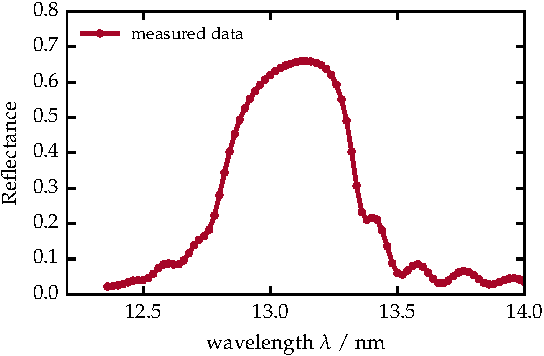
\includegraphics{img/PTB17_reflectance_AOI_15}
\caption{Spectrally resolved reflectance of the Mo/B$_4$C/Si/C multilayer sample. The measurement was conduced under a fixed angle of incidence $\alpha_i = 15.0^\circ$.}
\label{ch_spec:fig_ptb17_reflectance_AOI_15}
\end{figure}

The reflectiviy curve shows a broad peak attaining its maximum value at a wavelength of approximately \nm{13.1}, which is lower than the design peak reflectance of \nm{13.5}. That is due to the different angle of incidence used in the experiment. Apart from the main peak, side fringes are visible. They originate from the superposition of waves being reflected at the top surface and the substrate interface. They are thus directly related to the total thickness of the multilayer coating and well known as \emph{Kiessig fringes} \cite{kiessig_interferenz_1931}. Based on the data obtained through this spectrally resolved reflectivity experiment, we shall attempt to reconstruct the unknown layer layout in the following sections. The nominal fabrication parameters serve as starting values for the analysis to build a reasonable model for the reconstruction.

The reconstruction of a given model based on the evaluation of \gls{euv} (or \gls{xrr}) reflectivity data is a well established method for the characterization of multilayer systems  \cite{lim_fabrication_2001, bajt_investigation_2001, braun_mo/si_2002}. In most cases a model is optimized applying gradient methods such as the Levenberg-Marquardt method \cite{levenberg_method_1944, marquardt_algorithm_1963}. Those optimization algorithms typically operate with a set of start parameters within the parameter space and iteratively improve an optimization functional, usually termed $\chi^2$, describing the sum of the squared absolute value of the difference between the theoretical calculation and the experimental data. This is done by calculating the gradient of a that functional in all directions in the parameter space and changing the parameters accordingly in direction of smaller $\chi^2$ values. This approach has the major disadvantage that the end result is strongly dependent on the choice of starting values and may not represent a global minimum of $\chi^2$ but only a local optimum. While estimations of the quality of the fit results within the (local) optimum are possible, no estimation can be given globally for the given model. For those reasons, this characterization strategy has only limited applicability and alternative approaches are required.

In contrast to those gradient methods, heuristic optimization algorithms exist. Instead of operating with predefined starting values, from which a gradient approach minimizes the $\chi^2$ functional, they operate distributed on the whole parameter space with often randomly initialized parameters within given boundaries, instead. In the following we shall apply those heuristic optimization routines to obtain the reconstruction of the Mo/B$_4$C/Si/C sample and elaborate their application to the characterization of multilayer systems in detail.

\subsection{Multilayer Model and Particle Swarm Optimization} \label{ch_spec:sec_multilayer_model_and_pso}
For the purpose of reconstructing the layer layout of the Mo/B$_4$C/Si/C sample, a parameterized model is needed entering the theoretical calculations to obtain the reflectivity curve according to the matrix algorithm. The model is largely based on prior knowledge available from the fabrication process. For the multilayer sample investigated here, the nominal layer design is known and a schematic representation is shown in Fig.~\ref{ch_spec:fig_Mo_B4C_Si_C_model}.
\begin{figure}[htbp]
    \def\svgwidth{0.7\textwidth}
    \fontfamily{fds}\selectfont\footnotesize
    \import{svg/}{mo_si_ptb17_model.pdf_tex}
    \caption{Model of the multilayer stack including the substrate and the capping layers. The periodic part is enclosed between the dashed lines with four layers in each period repeated $N=64$ times. The capping period does not include an interdiffusion layer but does reflect the natural oxidation through the addition of a SiO$_2$ layer.}
    \label{ch_spec:fig_Mo_B4C_Si_C_model}
\end{figure}
As introduced above, the multilayer coating consists of a periodic arrangement of four layers replicated 64 times. With the top period being different from the others through the missing carbon interdiffusion layer on the top surface. Since the sample was exposed to ambient conditions, a passivation of the top silicon surface through oxidation has to be taken into account through a silicondioxide layer. The parameterization of that model is given by the thicknesses of each layer within one period as well as for the capping silicondioxide layer. Each of the deposited layers may vary in density with respect to the bulk density of that material \cite{braun_mo/si_2002}, which also needs to be reflected in the model. Finally, the N{\'e}vot-Croce factor $\sigma$ accounting for roughness and interdiffusion at the interfaces as introduced in chapter \ref{ch_theo} is also included. The required optical constants, i.e.~the indices of refraction, of the respective materials in the relevant spectral range are taken from tabulated values by \textcite{henke_x-ray_1993} and are used for the theoretical calculations based on the matrix algorithm. A full list of the model parameters for the multilayer sample can be found in table~\ref{ch_spec:tbl_mo_b4c_si_c_multilayer_parameters} together with physically plausible limits for each of the parameters. Due to the fact that the \gls{euv} reflectivity curve shown in Fig.~\ref{ch_spec:fig_ptb17_reflectance_AOI_15} shows the first order Bragg peak of the layer system, none of the layers can be thicker than \nm{7}, i.e.~in the order of half of the wavelength. The barrier layers were designed to attain thicknesses below \nm{1}. The density of the various materials within this model was constrained to values between $\SI{50}{\percent}$ and $\SI{100}{\percent}$ with respect to their bulk density. This is introduced to take into account reduced layer densities due to the amorphous state of the deposited layers. Through possible defects in an amorphous layer compared to a crystalline structure, the bulk density may not be attained. A layer with a density above the bulk density, on the other hand, is unlikely. Due to the high peak reflectance close to the theoretical limit of the multilayer sample in the \gls{euv} measurement, the maximum value of the N{\'e}vot-Croce factor was limited to be below $\sigma \leq \nm{2}$. With its upper limit, the measured peak reflectance can not be attained within this model thus not limiting the generality.
\begin{table*}
\centering
\caption{Multilayer parametrization and parameter limits}
\label{ch_spec:tbl_mo_b4c_si_c_multilayer_parameters}
\begin{tabular}{@{}llll@{}}
\toprule
Parameter & Definition & Lower bound & Upper bound\\ \midrule
$d_\text{Mo}$ / nm & Mo layer thickness & $0.0$& $7.0$\\ 
$d_\text{Si}$ / nm & Si layer thickness& $0.0$& $7.0$\\ 
$d_\text{C}$ / nm &C buffer layer thickness& $0.0$ & $5.0$\\ 
$d_\text{B$_4$C}$ / nm &B$_4$C buffer layer thickness&$0.0$ & $5.0$\\ 
$\sigma$ / nm & N\'{e}vot-Croce parameter& $0.0$& $2.0$\\ 
&(identical for all interfaces)&&\\
$\rho_\text{Mo}$ &Mo density w.r.t.~bulk density & $0.5$& $1.0$\\ 
$\rho_\text{Si}$ &Si density w.r.t.~bulk density& $0.5$& $1.0$\\ 
$\rho_\text{C}$ &C density w.r.t.~bulk density& $0.5$& $1.0$\\ 
$\rho_\text{B$_4$C}$ &B$_4$C density w.r.t.~bulk density& $0.5$& $1.0$\\
\midrule
\multicolumn{4}{c}{Capping layer}\\
\midrule
$d_\text{SiO$_2$(cap)}$ / nm & SiO$_2$ capping layer thickness & $0.0$&$5.0$ \\ 
$\rho_\text{SiO$_2$(cap)}$& $=\rho_\text{Si}$ (identical to Si density)& & \\
 \bottomrule
\end{tabular}
\end{table*}

\paragraph{The minimization functional and particle swarm optimization}
As introduced above, the reconstruction of the model for the multilayer is an optimization problem. Based on the measured reflectivity data an optimization functional defines the goodness of the model with respect to the measured data. The quality is asserted based on the method of least squares \cite{legendre_nouvelles_1805, gauss_theoria_1809, birge_calculation_1932} and the functional is defined as the reduced $\tilde{\chi}^2$
\begin{align}
\tilde{\chi}^2 = \frac{1}{M-P} \bigg[\sum\limits_{m} \frac{(I_m^\text{model} 
- I_m^\text{meas})^2}{\tilde{\sigma}_m^2} \bigg] \text{,} 
\label{ch_spec:eqn_reduced_chi_squared}
\end{align}
where $M$ is the number of measurement points, $P$ is the number of parameters used in the model, $I_m^\text{model}$ is the calculated intensity for the corresponding measurement point with index $m$ having the measured intensity $I_m^\text{meas}$. The calculated intensity fur the \gls{euv} reflectivity curve above $I_m^\text{model}$ follows directly from the matrix algorithm and the quantity $R$ in Eq.~\eqref{ch_theo:eqn_refl_trans_ML} in chapter~\ref{ch_theo}. Each point is calculated based on the angle of incidence and wavelength associated with measurement point $m$. The experimental uncertainty for each measurement point is described by $\tilde{\sigma}_m$.

For the minimization of the functional in Eq.~\eqref{ch_spec:eqn_reduced_chi_squared} we apply a global optimization algorithm known as \gls{pso} \cite{kennedy_particle_2011}. In contrast to the aforementioned gradient based methods, the \gls{pso} operates on the whole parameter space as defined by the upper and lower parameter limits, which are given in table~\ref{ch_spec:tbl_mo_b4c_si_c_multilayer_parameters} for the particular example here, without specific starting parameters influencing the convergence result. We implemented the \gls{pso} algorithm based on the draft by \textcite{carlisle_off--shelf_2001}. The basic mechanism of the algorithm is the definition of a swarm of individual particles, which are initialized randomly distributed across the allowed parameter space. Initially, each of those particles calculates the minimization functional at its random position retaining that result including a random start velocity. In an iterative process, the global best solution (``social component'') found as well as the individual best solution (``cognitive component'') of each particle are used to calculate an updated and weighted velocity vector within the parameter space for each particle. Within that iteration each of the particle thus moves to a new position, where the minimization functional is again evaluated and compared the the individual and global best solutions. If a better value is found, the respective retained results are updated with the new value and the next iteration is performed. While following that process the particles eventually converge to the global best solution, which may or may not be the global best optimum of the whole optimization problem. Due to the combination of social and cognitive component, fast convergence into a local optimum can be avoided. The state of full convergence is reached, when either all particles occupy the same place in the parameter space or if stagnation is reached. Due to the heuristic nature of the algorithm, it may happen that the global best optimum found is not necessarily the global minimum of the optimization problem. The result may be verified, however, by repeated application of the algorithm or simply by reaching a satisfactory solution through comparison of the measured and calculated curves and thus small $\tilde{\chi}^2$ values.

\paragraph{Model reconstruction based on the \gls{euv} reflectivity data}
We have applied this optimization procedure to the Mo/B$_4$C/Si/C sample and the measured \gls{euv} reflectivity curve. The fit result is shown together with the measured data in Fig.~\ref{ch_spec:fig_ptb17_reflectance_AOI_15_fitted}.
\begin{figure}[htbp]
\centering
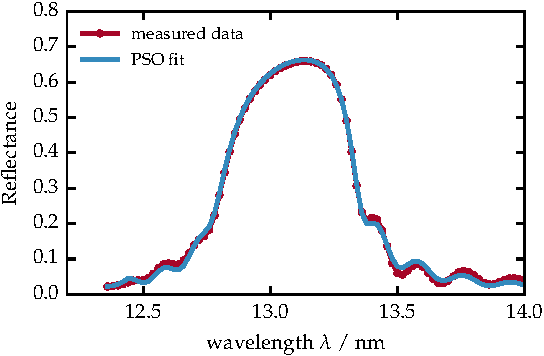
\includegraphics{img/PTB17_reflectance_AOI_15_fitted}
\caption{Theoretical reflectance curve based on the optimal model parameters obtained from the particle swarm optimization.}
\label{ch_spec:fig_ptb17_reflectance_AOI_15_fitted}
\end{figure}
The parameter results are listed in table~\ref{ch_spec:tbl_mo_b4c_si_c_multilayer_parameters_results}. The solution does indeed provide a very good agreement with the measured data. However, by repeated evaluation of the \gls{pso} procedure, significantly different results for the optimal parameter set with comparable agreement and very similar $\tilde{\chi}^2$ values were found. Three examples are listed in table~\ref{ch_spec:tbl_mo_b4c_si_c_multilayer_parameters_results} with their respective $\tilde{\chi}^2$ values. Clearly, this is no desirable situation, since no definite answer of the actual thicknesses found in the sample can be made. To complete the characterization additional methods of model verification are thus required. We shall therefore discuss an additional approach to the optimization problem in the following section on how the model validity and the information content of the measured data can be asserted based on the example of the \gls{pso} results obtained here.
\begin{table*}[htbp]
\centering
\caption{Results for the optimized parameters based on the \gls{pso} of the \gls{euv} reflectivity for the Mo/B$_4$C/Si/C sample.}
\label{ch_spec:tbl_mo_b4c_si_c_multilayer_parameters_results}
\begin{tabular}{@{}lllll@{}}
\toprule
Parameter & Definition& \multicolumn{3}{c}{PSO results}\\ \midrule
$d_\text{SiO$_2$(cap)}$ / nm &SiO$_2$ capping layer thickness& $3.194$ & $3.418$& $3.558$\\
$d_\text{Mo}$ / nm &Mo layer thickness&  $2.460$ & $2.748$& $ 3.082$\\
$d_\text{Si}$ / nm &Si layer thickness& $2.421$ & $2.617$& $1.997$\\ 
$d_\text{C}$ / nm &C buffer layer thickness& $0.811$ & $0.709$& $0.818$\\ 
$d_\text{B$_4$C}$ / nm &B$_4$C buffer layer thickness& $1.308$ & $0.923$& $1.129$\\ 
$\sigma$ / nm &N\'{e}vot-Croce parameter& $0.322$ & $0.249$& $0.177$\\
$\rho_\text{Mo}$ &Mo density w.r.t.~bulk density& $0.989$ & $0.919$& $0.944$\\ 
$\rho_\text{Si}$ &Si density w.r.t.~bulk density& $0.883$ & $0.974$& $0.749$\\ 
$\rho_\text{C}$ &C density w.r.t.~bulk density& $0.833$ & $ 0.971$& $0.608$\\ 
$\rho_\text{B$_4$C}$ &B$_4$C density w.r.t.~bulk density& $0.909$ & $0.973$& $0.936$\\
 \midrule
 $\tilde{\chi}^2$ & reduced $\chi^2$ value & $71.46$ & $71.56$ & $73.08$ \\
 \bottomrule
\end{tabular}
\end{table*}

\subsection{Model Uniqueness and Maximum Likelihood Estimation} \label{ch_spec:sec_maximum_likelihood}
With the ambiguous reconstruction result of the previous section, the demand for a verification of the model with respect to the measured data becomes apparent. To clarify the problem of uniqueness of the solution, it is instructive to investigate the influence of the individual model parameters on the theoretical reflectivity curve. In Fig.~\ref{ch_spec:fig_mo_si_parameter_influence} we varied a subset of the parameters starting from the \gls{pso} solution from Sec.~\ref{ch_spec:sec_multilayer_model_and_pso}. In each of the subfigures, one parameter or a quotient of parameters is varied while all others are kept fixed.
\begin{figure*}[htbp]
\centering
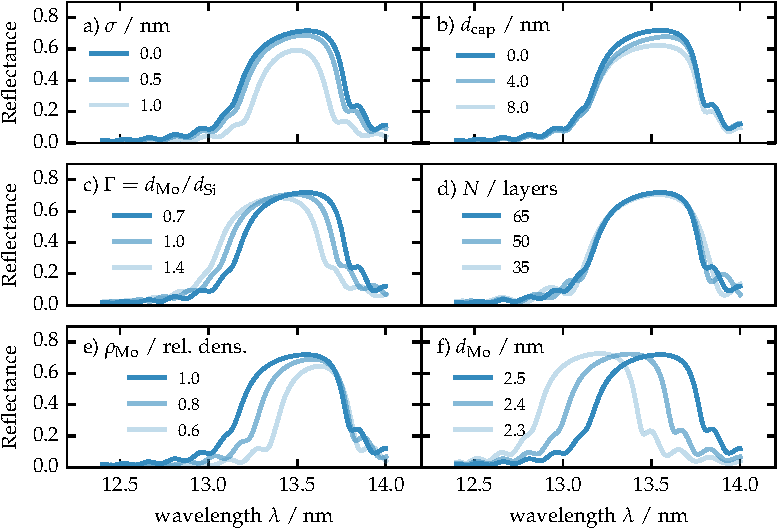
\includegraphics{img/parameter_influence}
\caption{Influence of the change of parameter model on the simulated \gls{euv} reflectivity curve. In each of the figures, all parameters were kept constant at the values listed in table~\ref{ch_spec:tbl_mo_b4c_si_c_multilayer_parameters_results} varying only the respective shown parameter.}
\label{ch_spec:fig_mo_si_parameter_influence}
\end{figure*}
By comparison of Fig.~\ref{ch_spec:fig_mo_si_parameter_influence}a, \ref{ch_spec:fig_mo_si_parameter_influence}b, \ref{ch_spec:fig_mo_si_parameter_influence}c and \ref{ch_spec:fig_mo_si_parameter_influence}e it becomes clear that a reduction of the peak reflectivity can originate in either a large roughness and interdiffusion parameter $\sigma$ or similarly from the thickness of the capping layer, the silicon to molybdenum layer thickness ratio of the molybdenum density. A reconstruction based on a single \gls{euv} reflectivity therefore intrinsically produces a highly ambiguous result with strong parameter correlations. The available data, a single \gls{euv} reflectivity curve in this case, does not allow for a unique set of parameters of the model minimizing the $\chi^2$ functional. In reality multiple solutions with very similar values for $\tilde{\chi}^2$ exist as shown above. Clearly, this raises the question of how accurately a reconstruction may be achieved here.

\paragraph{Maximum likelihood}
A solution of the aforementioned problem requires to determine the value of $\tilde{\chi}^2$ in vicinity of the \gls{pso} solution or possibly the whole parameter space. We approach this by numerically sampling the functional based on a \gls{mcmc} method \cite{goodman_ensemble_2010}. An application of this technique to the design process of multilayer mirrors has been demonstrated by \textcite{hobson_markov-chain_2004}. In our case, the match of model and experimental result is evaluated based on a non-centered $\chi^2$ distribution assuming independent measurements. We further assume that any measured point is distributed around the actual reflectivity curve following a Gaussian distribution, i.e.~we assume Gaussian uncertainties for the experiment. The corresponding probability density function for a measurement result matching with the actual reflectivity curve, which is assumed to be obtainable exactly through the theoretical calculation, is then of Gaussian form \cite{abramowitz_handbook_1964}. Thus, the likelihood that the measured values match with the theoretical curve under the assumption that the model is correct is proportional to
\begin{align}
 L(E | M(\vec{x})) \propto \exp \big(- \tilde{\chi}^2(\vec{x}) / 2 \big) \text{,} \label{ch_spec:eqn_likelihood_experiment_vs_model}
\end{align}
where $E$ denotes the experiment, i.e.~the measured data and $M(\vec{x})$ represents the model given through parameter set $\vec{x}$, e.g.~the parameters of the model in table~\ref{ch_spec:tbl_mo_b4c_si_c_multilayer_parameters}. In our case however, we seek to evaluate the likelihood $L(M(\vec{x}) | E)$ that the model $M(\vec{x})$ with a given set of parameters $\vec{x}$ is valid assuming the experiment $E$ yields the correct curve (the so called ``posterior distribution''). Those two quantities are linked through the Bayesian theorem \cite{bayes_essay_1763, milton_introduction_2002} stating
\begin{align}
 L(M(\vec{x}) | E) \propto L(E | M(\vec{x})) L(M(\vec{x})) \text{,} \label{ch_spec:eqn_bayesian_theorem}
\end{align}
where $L(M(\vec{x}))$ denotes the likelihood for the model to be valid for a specific set of parameters $\vec{x}$ (the so called ``prior distribution''). The prior distribution does contain any prior knowledge about the model and allowed parameters. For the example of the model parameters in table~\ref{ch_spec:tbl_mo_b4c_si_c_multilayer_parameters}, the prior distribution is $L(M(\vec{x})) \rightarrow -\infty$ for any parameter set outside the listed boundaries and $L(M(\vec{x})) = 1$ everywhere else. In addition, we limit the maximum total period thickness, i.e.~the sum of all layers in one period to only allow the appearance of the first Bragg peak within the measured spectral range through the same condition. Combining Eq.~\eqref{ch_spec:eqn_likelihood_experiment_vs_model} and Eq.~\eqref{ch_spec:eqn_bayesian_theorem} then yields the likelihood functional
\begin{align}
 L(\vec{x}) = L(M(\vec{x}) | E) \propto \exp \big(- \tilde{\chi}^2(\vec{x}) / 2 \big) L(M(\vec{x})) \text{.} \label{ch_spec:eqn_likelihood}
\end{align}

Solving the optimization problem posed in the previous section within this context is then, equivalently to the minimization of $\tilde{\chi}^2$, the maximization of the likelihood $L(\vec{x})$. The \gls{mcmc} method poses a statistical approach on evaluating (mapping) the likelihood across the parameter space within the previously defined limits as in the \gls{pso} approach. It was proven that after a theoretical number of infinite iterations, the distribution of the individual samples within the \gls{mcmc} algorithm, corresponds to the likelihood functional in Eq.~\eqref{ch_spec:eqn_likelihood} \cite{cox_theoretical_1979, mackay_information_2003}. With a limited number of iterations, a numerical approximation of that distribution is obtained after reaching an equilibrium state in the algorithm \cite{foreman-mackey_emcee:_2013}. It thus yields an alternative method on solving the optimization problem by extracting the maximum likelihood from the final result. However, in addition to the maximum value, the likelihood distribution in parameter space is obtained allowing to extract confidence intervals for each of the parameters. Thereby, the aforementioned ambiguity of solutions can be quantified within the defined model and the available experimental data. The confidence intervals are defined as the one- or two-sigma standard deviations of the respective distributions for each parameter.

\paragraph{Confidence intervals for the Mo/B$_4$C/Si/C sample}
We have applied an existing implementation of the \gls{mcmc} algorithm by \textcite{foreman-mackey_emcee:_2013} to the \gls{euv} measurement of the Mo/B$_4$C/Si/C sample in Fig.~\ref{ch_spec:fig_ptb17_reflectance_AOI_15} with the model in Fig.~\ref{ch_spec:fig_Mo_B4C_Si_C_model}. The likelihood, as defined in Eq.~\eqref{ch_spec:eqn_likelihood} with the $\tilde{\chi}^2$ functional from Eq.~\eqref{ch_spec:eqn_reduced_chi_squared}, is sampled in a high-dimensional space depending on the number of parameters in the model. We therefore need to project the distribution for each parameter by marginalizing over all other parameters. Alternatively, two-parameter correlations can be visualized by projecting on a two-dimensional area, again marginalizing across all other parameters. The projection for the Si and Mo layer thicknesses are shown in Fig.~\ref{ch_spec:fig_ptb17_MCMC_d_Mo_vs_d_Si}b and \ref{ch_spec:fig_ptb17_MCMC_d_Mo_vs_d_Si}c. In both cases, a well defined distribution is obtained. In the two-dimensional projection in Fig.~\ref{ch_spec:fig_ptb17_MCMC_d_Mo_vs_d_Si}a, no correlations are apparent and a two-dimensional Gaussian-like shape results.
\begin{figure*}[htbp]
\centering
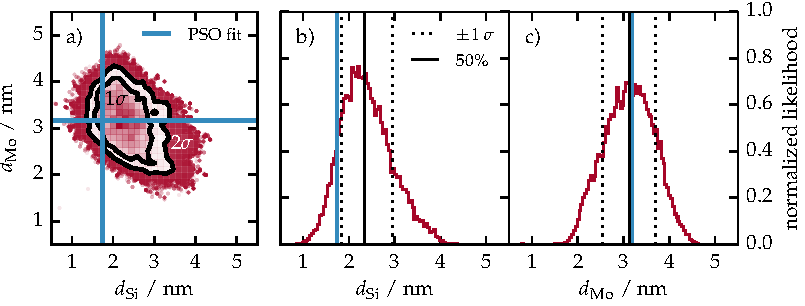
\includegraphics{img/PTB17_MCMC_d_Mo_vs_d_Si}
\caption{Results of the maximum likelihood estimation obtained via the \gls{mcmc} procedure. a) Two dimensional projection of the likelihood distribution for the parameter pair $d_\text{Si}$ and $d_\text{Mo}$. The projection was obtained by marginalizing over all other parameters of the model. The black contours indicate the areas for one and two standard deviations (one and two sigma contours). The blue lines in all three sub-figures indicate the best parameter set found with the \gls{pso} method. b) One dimensional projection of the likelihood distribution for the silicon layer thickness $d_\text{Si}$. The solid black line marks the center position ($50\%$ percentile) of the distribution. The dotted lines are the limits of one standard deviation. c) The one dimensional distribution similarly to b) for the molybdenum layer thickness.}
\label{ch_spec:fig_ptb17_MCMC_d_Mo_vs_d_Si}
\end{figure*}
\begin{figure*}[htbp]
\centering
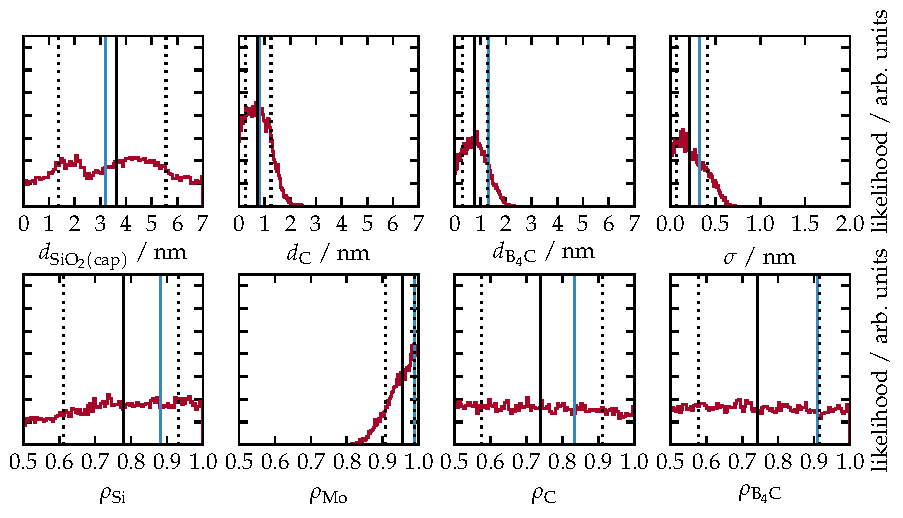
\includegraphics{img/PTB17_MCMC_other_params}
\caption{In analogy to Fig.~\ref{ch_spec:fig_ptb17_MCMC_d_Mo_vs_d_Si}b and \ref{ch_spec:fig_ptb17_MCMC_d_Mo_vs_d_Si}c the one dimensional projections of the likelihood distribution estimation for the Mo/B$_4$C/Si/C sample are shown for the remaining parameters of the model with the \gls{pso} result, the center value and one standard deviation.}
\label{ch_spec:fig_ptb17_MCMC_other_params}
\end{figure*}
In all cases, the one-sigma standard deviations for Gaussian distributions are shown together with the weighted center, i.e.~the $50$th percentile. The \gls{pso} result is also indicated, which is compatible with the one sigma standard deviation, but does not match the center of the likelihood result. The reason for that lies in higher order correlations of the parameters. In Fig.~\ref{ch_spec:fig_ptb17_MCMC_other_params}, all one-dimensional projections of the likelihood distribution are shown for all remaining parameters. Clearly, while a reasonably small confidence interval (again, one standard deviation for all distributions) can be found for the thickness of the carbon and boroncarbite layers, the off-center value for the silicon thickness of the PSO result in Fig.~\ref{ch_spec:fig_ptb17_MCMC_d_Mo_vs_d_Si}c is compensated by a larger than center value for the boroncarbite layer in Fig.~\ref{ch_spec:fig_ptb17_MCMC_other_params}. Thus, the thicknesses are correlated and are no independent model parameters. Nevertheless, confidence intervals can be obtained within the given model and the given prior (the boundaries listed in table~\ref{ch_spec:tbl_mo_b4c_si_c_multilayer_parameters}) and are listed accordingly in table~\ref{ch_spec:tbl_mo_b4c_si_c_multilayer_mcmc_results} for one and two standard deviations. Within the allowed boundaries, some parameters remain entirely undefined with similar likelihood for any parameter value, such as the SiO$_2$ capping layer thickness, the silicon, carbon and boroncarbite relative densities. Their corresponding total confidence intervals thus cover almost exactly $68.2\%$ (one standard deviation) and $95.4\%$ (two standard deviations) of the allowed respective parameter range. Hence, with respect to the model defined and the measured \gls{euv} reflectivity curve, no reliable value for those sample properties can be determined.
\begin{table*}[htbp]
\centering
\caption{\gls{mcmc} results obtained by the analysis of the \gls{euv} reflectivity for the Mo/B$_4$C/Si/C sample. The center values ($50\%$ percentile) together with confidence intervals (c.i.) of one and two standard deviations are shown.}
\label{ch_spec:tbl_mo_b4c_si_c_multilayer_mcmc_results}
\begin{tabular}{@{}lllll@{}}
\toprule
Parameter & PSO result & center value & $1 \sigma$ c.i.& $2 \sigma$ c.i.\\ \midrule
$d_\text{SiO$_2$(cap)}$ / nm & $3.194$& $3.677 $&$({-2.252}/{+1.944})$ & $({-3.407}/{+3.108})$ \\
$d_\text{Mo}$ / nm &  $2.460$& $3.137$&$({-0.587}/{+0.560})$ & $({-1.054}/{+1.016})$ \\
$d_\text{Si}$ / nm & $2.421$& $2.338$&$({-0.497}/{+0.616})$ & $({-0.916}/{+1.294})$ \\
$d_\text{C}$ / nm& $0.811$ & $0.744$&$({-0.477}/{+0.510})$ & $({-0.696}/{+0.971})$ \\
$d_\text{B$_4$C}$ / nm & $1.308$& $0.782$&$({-0.471}/{+0.511})$ & $({-0.722}/{+0.973})$ \\
$\sigma$ / nm & $0.322$& $0.214$&$({-0.143}/{+0.201})$ & $({-0.204}/{+0.347})$\\
$\rho_\text{Mo}$ & $0.989$& $0.953$&$({-0.048}/{+0.034})$ & $({-0.094}/{+0.045})$ \\
$\rho_\text{Si}$ & $0.883$& $0.782$&$({-0.167}/{+0.147})$ & $({-0.264}/{+0.208})$ \\
$\rho_\text{C}$ & $0.833$& $0.739$&$({-0.164}/{+0.175})$ & $({-0.228}/{+0.249})$ \\
$\rho_\text{B$_4$C}$ & $0.909$& $0.741$&$({-0.162}/{+0.172})$ & $({-0.230}/{+0.247})$ \\
 \bottomrule
\end{tabular}
\end{table*}

It should be noted, that the given center values here are not a good solution to the optimization problem. The reason for that is, that the parameters are highly correlated. The center values of the one-dimensional projections may therefore not be suitable parameters for the model based on the low amount of data available. A valid optimization result can therefore only be obtained by either applying the \gls{pso} routine or by iterative application of the \gls{mcmc} procedure. The latter may be achieved by fixing single parameters according to their maximum likelihood value  found in the previous iteration and obtaining the resulting likelihood distributions for the remaining parameters according to that restricted prior distribution.

The results listed in table~\ref{ch_spec:tbl_mo_b4c_si_c_multilayer_mcmc_results} serve as the model parameters for the analysis of diffuse scattering from the Mo/B$_4$C/Si/C sample in chapter~\ref{ch_diff}.

\section{Molybdenum Thickness Variation in Mo/Si/C Multilayers} \label{ch_spec:sec_mo_si_c}
For the engineering of a near-normal incidence mirror, the ratio of molybdenum layer thickness to total period thickness has a clear impact on the reflectivity curve as seen from the theoretical simulations in Fig.~\ref{ch_spec:fig_mo_si_parameter_influence}c. Studies have shown, that an optimal value for high reflectivity is achieved by depositing $40\%$ molybdenum layer thickness $d_\text{Mo}$ with respect to the total period thickness $D$ \cite{bajt_investigation_2001,braun_mo/si_2002}. During the deposition process, the layer of molybdenum grows in thickness and at a certain threshold, crystallites may begin to form \cite{verhoeven_ion_1992,bajt_investigation_2001} inside the layer. Those may affect the interface morphology of the layer system at the boundaries to the molybdenum layer and possibly at further interfaces through correlation effects. This potentially increases the roughness and thus the loss of specularly reflected radiation to diffuse scatter.

In the following we shall apply and extend the reconstruction procedure discussed in the above section to the problem of multilayer sample systems deposited with varying molybdenum layer thicknesses from sample to sample. The samples discussed in this section were designed to investigate the impact of the crystallization on the performance on Mo/Si multilayer mirrors systems. Two sets of samples were fabricated. One with the standard magnetron deposition technique, which we shall refer to as \emph{unpolished samples} and another set with an additional ion polishing step applied within the deposition of each period to counteract the roughening expected from the crystallization process. Consequently, the latter samples are referred to as \emph{polished samples}. Both sets were deposited with linearly increasing molybdenum thickness across all periods from sample to sample. The details of the sample layout and the reflectivity measured from each sample are described in detail in Sec.~\ref{ch_spec:sec_mo_si_c_sample_systems_and_experimental}. 

The goal of this investigation is to analyze the interface morphology in each sample and asses the effect of the crystallization process and the polishing treatment. For that, the nominally deposited layer thicknesses are verified and the model including the determination of the densities and the interdiffusion and roughness parameters is reconstructed in Sec.~\ref{ch_spec:sec_MoSi_euv_xrr_combined} based on specular analytic experiments and the application of the \gls{pso} and the \gls{mcmc} methods introduced above. The findings are shown and discussed in Sec.~\ref{ch_spec:sec_mo_si_c_results}. The results presented here are part of the published work in \fullcite{haase_interface_2017}.

\subsection{Sample systems and experimental procedure} \label{ch_spec:sec_mo_si_c_sample_systems_and_experimental}
Two sets of several samples of Mo/Si/C multilayer mirrors with C interdiffusion barriers with thicknesses of nominally below \nm{0.5} at the Mo on Si interfaces (a detailed figure of the model for those samples is given below in Fig.~\ref{ch_spec:fig_model_unpolished_and_polished_samples} of the following sections) were prepared. As mentioned above, the samples under investigation here were fabricated with increasing relative Mo thickness from sample to sample while keeping the nominal period thickness $D\approx 7$ nm constant by correspondingly reducing the silicon layer thickness. In this study, we investigate two sets of samples. In the first set, the magnetron sputtered layers were deposited one after another for each sample. In the second set, during deposition, an additional polishing process was used once during sputtering each period to counteract the possible roughening due to the crystallization. The nominal values of the molybdenum layers in the two sample sets are listed in table~\ref{ch_spec:tbl_mo_si_thickness_nominal}.
\begin{table}[htbp]
\centering
\caption{List of nominal molybdenum layer thicknesses in the two sample sets. Both sets were fabricated with a equidistant increase in thickness from \nm{1.70} to \nm{3.05} with 9 unpolished and 10 polished samples.}
\label{ch_spec:tbl_mo_si_thickness_nominal}
\begin{tabular}{@{}ll@{}}
\toprule
nominal $d_\text{Mo}$ / nm & nominal $d_\text{Mo}$ / nm\\ 
(unpolished samples) & (polished samples) \\
\midrule
$1.70$& $1.70$\\ 
$1.85$& $1.85$\\ 
$2.00$ & $2.00$\\ 
$2.15$ & $2.15$\\ 
$2.30$& $2.30$\\ 
$2.45$& $2.45$\\ 
$2.60$& $2.60$\\ 
$2.75$ & $2.75$\\ 
$2.90$ & $2.90$\\ 
-& $3.05$\\ 
 \bottomrule
\end{tabular}
\end{table}

Spectrally resolved \gls{euv} reflectivity curves at an angle of incidence from the surface normal of $\alpha_i=\SI{15}{\degree}$ and in the wavelength range from \nm{12.4} to \nm{14.0} have been measured for all samples at the \gls{euvr} beamline at the \gls{mls}. The data obtained is shown in Fig.~\ref{ch_spec:fig_EUV_reflectivity_unpolished_and_polished} sorted by the nominal molybedum layer thickness.
\begin{figure}[htbp]
\centering
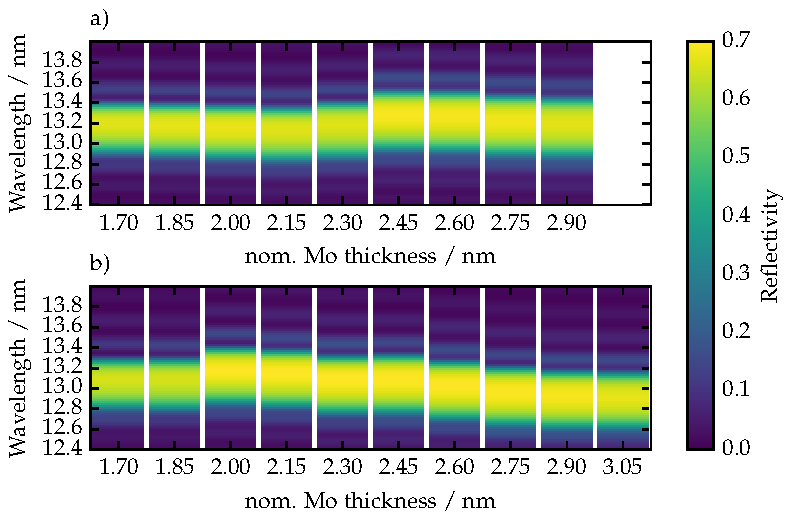
\includegraphics[width=0.7\textwidth]{img/MoSi_EUV_reflectivity}
\caption{a) Measured reflectivity curves for the unpolished samples across the wavelength at a fixed angle of incidence of $\alpha_i = 15^\circ$ from the surface normal. The nine samples differ by the nominal Mo layer thickness indicated at the bottom axis. b) Measured reflectivity curves of the ten polished samples measured under the same conditions as for the first sample set.}
\label{ch_spec:fig_EUV_reflectivity_unpolished_and_polished}
\end{figure}
The reflectivity curves in Fig.~\ref{ch_spec:fig_EUV_reflectivity_unpolished_and_polished}a and Fig.~\ref{ch_spec:fig_EUV_reflectivity_unpolished_and_polished}b have the characteristic curve shape of periodic \gls{euv} multilayer mirrors with a main broad maximum and side fringes, very similar to the mirror sample discussed in Sec.~\ref{ch_spec:sec_PTB17} above. In direct comparison of the measured reflectivity data, shifts of the peak center position are clearly visible. As illustrated in Fig.~\ref{ch_spec:fig_mo_si_parameter_influence} above, several properties of a multilayer stack, e.g.~molybdenum content and period thickness, contribute to such a difference. Clear differences in the peak reflectance value can also be observed in the two subfigures, with strong increases at $d_\text{Mo}^\text{nom} = \nm{2.45}$ for the unpolished set and at $d_\text{Mo}^\text{nom} = \nm{2.00}$ for the polished set. In all samples the only nominal difference, i.e.~the only parameter changed during the deposition process, is the relative molybdenum thickness. The increase in reflectance, peak broadening and the jump of the peaks center position are therefore indicators for an abrupt change in the multilayer properties.

For the purpose of obtaining additional information about the samples, in addition to the \gls{euv} reflectivity curves above, all samples were measured after deposition using a lab-based Cu-K$_\alpha$ X-ray diffractometer at the Fraunhofer IWS Dresden, Germany. The \gls{xrr} data is shown in Fig.~\ref{ch_spec:fig_MoSi_XRR} for the set of unpolished and polished samples in direct comparison.
\begin{figure*}[htbp]
\centering
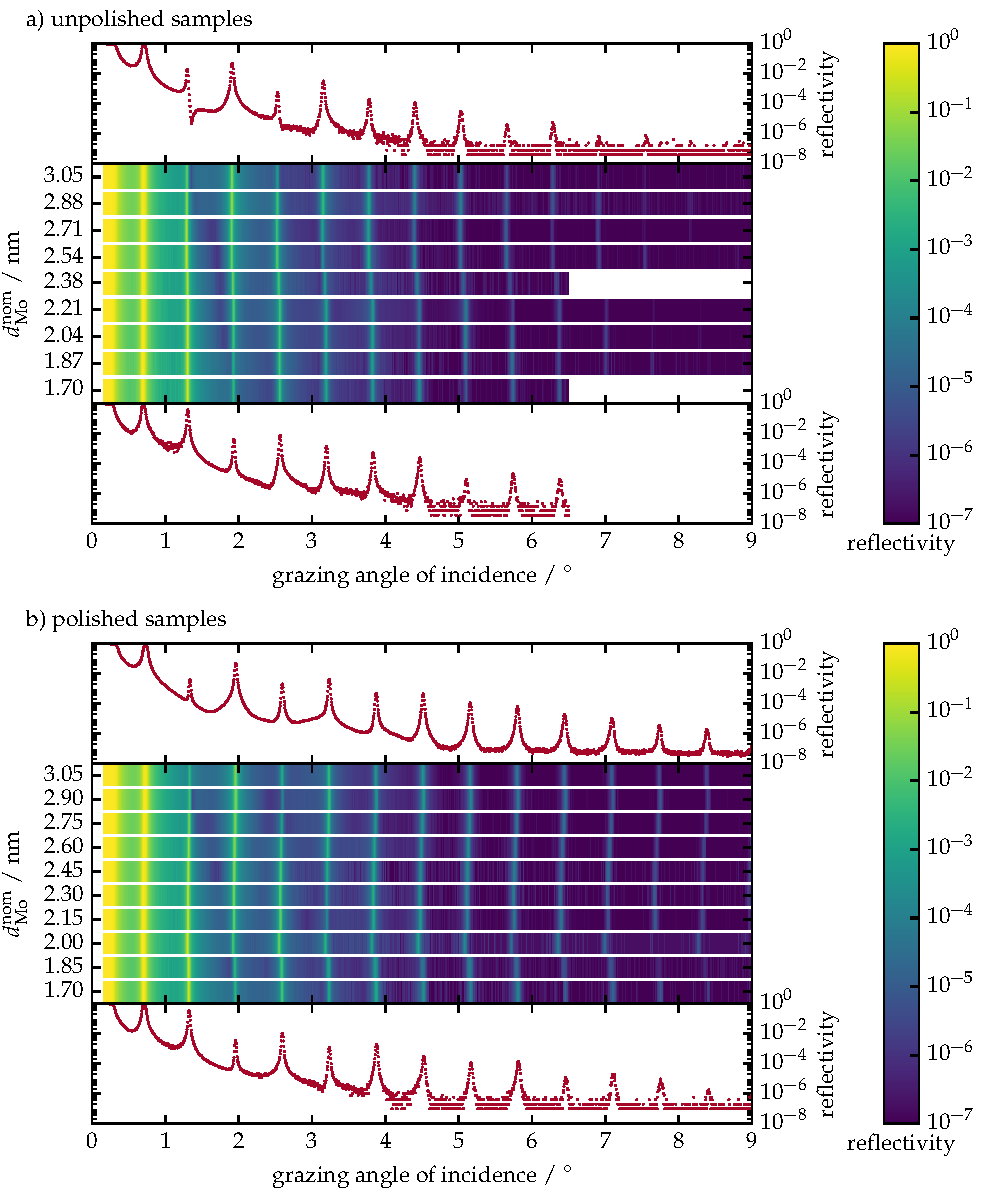
\includegraphics[width=\textwidth]{img/XRR_MoSi}
\caption{\gls{xrr} data for all unpolished and polished samples shown in dependence on the nominal molybdenum layer thickness $d_\text{Mo}^\text{nom}$ and the grazing angle of incidence $\alpha_i^\text{GI}$ at the Cu-K$_\alpha$ photon energy of $E_\text{ph} = \ev{8048}$. In each of the subfigures a) and b) the \gls{xrr} measurements for the sample with smallest and largest $d_\text{Mo}^\text{nom}$ are shown on the bottom and the top of the subfigure, respectively. In between, the \gls{xrr} curves are shown in as a color map plot.}
\label{ch_spec:fig_MoSi_XRR}
\end{figure*}
The position of the Bragg peaks and their respective intensity contain additional information on the layer stack thicknesses and its interface properties. In both cases, shifts of the peak positions and intensities similar to those observed in the \gls{euv} curves become apparent. Especially the higher orders towards larger grazing incidence angles show distinct differences. In addition, in direct comparison of the \gls{xrr} curves for the respective sample with $d_\text{Mo}^\text{nom} = \nm{3.05}$ from the unpolished and polished sets (on the top of Fig.~\ref{ch_spec:fig_MoSi_XRR}a and Fig.~\ref{ch_spec:fig_MoSi_XRR}b), a higher intensity for higher-order Bragg peaks above grazing angles of incidence of $\alpha_i^\text{GI} > \SI{7}{\degree}$ can be observed for the polished sample. This hints towards an improved interface definition and sharpness due to the polishing process and consequently a lower roughness or interdiffusion.

In the following section we shall analyze the \gls{euv} and \gls{xrr} data discussed here to reconstruct a model of the samples using the \gls{mcmc} approach introduced in Sec.~\ref{ch_spec:sec_reconstruction_PTB17} in order to verify the observations made here.

\subsection{Combined Analysis of X-ray and EUV reflectance} \label{ch_spec:sec_MoSi_euv_xrr_combined}
To obtain the actual layer thicknesses in the samples, we analyzed the data of the \gls{euv} reflectivity and \gls{xrr} experiments and reconstructed these parameters by combined analysis of the measured data. The reflectivity curves for the different measurements are calculated by introducing a model for the multilayer system and applying the matrix formalism described in detail in the theory part of this thesis, Sec.~\ref{ch_theo:sec_matrix_algorithm}.

The thicknesses of the Mo layers inside the stack were varied nominally from $1.7$ nm to $3.05$ nm from sample to sample, where the unpolished sample set lacks the last nominal thickness. The stacking of the different layers in the multilayer consists of the Mo and Si layers, as well as an additional C buffer layer at the Mo on Si interface to prevent interdiffusion. For the Si on Mo interfaces, no buffer layers were included since interdiffusion is usually less in this case \cite{petford-long_highresolution_1987}. However, for the theoretical description of the sample stack we consider an additional MoSi$_2$ layer in the model, which is well known to form during the deposition process \cite{bajt_investigation_2001}. The full model used in the reconstruction is illustrated in Fig.~\ref{ch_spec:fig_model_unpolished_and_polished_samples} with the thickness parameters for each layer.
\begin{figure}[htbp]
    \def\svgwidth{0.7\textwidth}
    \fontfamily{fds}\selectfont\footnotesize
    \import{svg/}{mo_si_iws_model.pdf_tex}
    \caption{Model of the multilayer stack including the substrate and the capping layers. The periodic part is enclosed between the dashed lines with four layers in each period repeated 49 times. The capping period does not include an interdiffusion layer but has a natural SiO$_2$ layer and a carbon-like layer accounting for contamination on the top surface.}
    \label{ch_spec:fig_model_unpolished_and_polished_samples}
\end{figure}
To account for any contamination on the top sample surface, an additional carbon-like layer as the upper most layer was considered. In addition to the thicknesses of each layer we also allowed for a variation of the layer density between $80\%$ and $100\%$ of the bulk density. The model parameters and their boundaries entering in the optimization procedure are listed in table~\ref{ch_spec:tbl_mo_si_c_multilayer_parameters}. Similar to the Mo/B$_4$C/Si/C in Sec.~\ref{ch_spec:sec_reconstruction_PTB17}, a N\'{e}vot-Croce damping factor was assumed to account for specular reflectivity loss due to interface imperfections. 
\begin{table*}
\centering
\caption{Parametrization of the Mo/Si/C multilayer samples with varying molybdenum layer thicknesses.}
\label{ch_spec:tbl_mo_si_c_multilayer_parameters}
\begin{tabular}{@{}llll@{}}
\toprule
Parameter & Definition & Lower bound & Upper bound\\ \midrule
$d_\text{Mo}$ / nm & Mo layer thickness & $0.0$& $4.5$\\ 
$d_\text{Si}$ / nm & Si layer thickness& $0.0$& $7.0$\\ 
$d_\text{C}$ / nm &C buffer layer thickness& $0.0$ & $0.6$\\ 
$d_\text{MoSi$_2$}$ / nm &MoSi$_2$ interdiffusion layer thickness&$0.0$ & $0.6$\\ 
$\sigma$ / nm & N\'{e}vot-Croce parameter& $0.0$& $0.5$\\ 
&(identical for all interfaces)&&\\
$\rho_\text{Mo}$ &Mo density w.r.t.~bulk density & $0.8$& $1.0$\\ 
$\rho_\text{Si}$ &Si density w.r.t.~bulk density& $0.8$& $1.0$\\ 
$\rho_\text{C}$ &C density w.r.t.~bulk density& $0.8$& $1.0$\\ 
$\rho_\text{MoSi$_2$}$ &MoSi$_2$ density w.r.t.~bulk density& $0.8$& $1.0$\\
\midrule
\multicolumn{4}{c}{Capping layer}\\
\midrule
$d_\text{C(cap)}$ / nm & C capping layer thickness & $0.0$&$3.0$ \\ 
$d_\text{SiO$_2$(cap)}$ / nm & SiO$_2$ capping layer thickness & $0.0$&$1.5$ \\ 
$\rho_\text{C(cap)}$ &C density w.r.t.~bulk density& $0.0$& $1.0$\\ 
$\rho_\text{SiO$_2$(cap)}$& $=\rho_\text{Si}$ (identical to Si density)& & \\
 \bottomrule
\end{tabular}
\end{table*}

\paragraph{Optimization functional and procedure} 
The data analysis was conduced similarly to the procedure described in Sec.~\ref{ch_spec:sec_reconstruction_PTB17}. However, for the samples studied here, two separate experiments and data sets were measured with the goal to improve the reconstruction of the model. Due to the increased amount of data through the additional \gls{xrr} measurements, a definition for a combined $\chi^2$ functional is required to allow an analysis based on both data sets. The two data sets, i.e.~the \gls{euv} and \gls{xrr} reflectivity curves have significantly different number of data points, which are not entirely independent of each other. In case of the \gls{xrr} curve increasing the number of data points, e.g.~by reducing the angular step size by half does not lead to better statistics due to systematic errors. Defining a $\chi^2$ functional as the total sum of all measured data point residuals, i.e.~both the \gls{euv} data and the \gls{xrr} data would therefore create an unwanted weighting due to the large amount of \gls{xrr} data points in comparison to far fewer \gls{euv} data points. To avoid this effect, we define the combined $\chi^2$ functional as the sum of the reduced $\tilde{\chi}^2$ functionals. The $\tilde{\chi}^2$ is equivalently defined to Eq.~\eqref{ch_spec:eqn_reduced_chi_squared} through,\begin{align}
\tilde{\chi}^2 = \frac{1}{M-P} \bigg[\sum\limits_{m} \frac{(I_m^\text{model} 
- I_m^\text{meas})^2}{\tilde{\sigma}_m^2} \bigg] \text{,}
\end{align}
for each of the datasets separately. The reduced $\tilde{\chi}^2$ can be interpreted as the average of the squared residuals of model prediction and experiment. Thereby, each experiment is reduced to a single comparable quantity. By the definition of
\begin{align}
\chi^2 = \tilde{\chi}^2_\text{EUV} +\tilde{\chi}^2_\text{XRR} \text{,}
\label{ch_spec:eqn_Mo_Si_C_total_chi_2}
\end{align}
we are therefore enabled to obtain confidence intervals for the parameters of the model, which represent a conservative (upper limit) estimation for the combined analysis of both experiments, similarly to the procedure for a single \gls{euv} curve as described in Sec.~\ref{ch_spec:sec_reconstruction_PTB17} above. The combined $\chi^2$ functional enters the likelihood through Eq.~\ref{ch_spec:eqn_likelihood}.

The solution to the inverse problem of reconstructing the optimal model parameters is conducted by minimizing  the $\chi^2$ functional (or equivalently maximizing the likelihood). To minimize the functional with respect to the best choice of parameters, we apply the \gls{mcmc} method as described above for the Mo/B$_4$C/Si/C sample system. We do not start with a \gls{pso} optimization, since the sample system is numerically simpler due to the decreased amount of layers and interfaces. The \gls{mcmc} method itself yields an optimization result, although slower in convergence, as mentioned in the discussion of the procedure above in Sec.~\ref{ch_spec:sec_maximum_likelihood}. As a starting point, again a random set of parameters is generated with respect to predefined boundaries listed in table~\ref{ch_spec:tbl_mo_si_c_multilayer_parameters}. The limits are chosen in reference to prior knowledge and physical plausibility. Confidence intervals for each value within the underlying model are estimated from the likelihood distribution resulting from the \gls{mcmc} as one standard deviation of the sample distribution in each parameter.

We shall discuss the results of the optimization procedure at the example of the unpolished sample with nominal molybdenum layer thickness of $d_\text{Mo}^\text{nom} = \nm{3.05}$. The results of the \gls{mcmc} maximum likelihood estimation for the other samples were found to show the same properties and the same findings discussed in the following with the only distinction of broader or even improved distributions in some cases. The latter causes the confidence intervals to be different for the respective parameters.

As a first step, the \gls{mcmc} procedure was performed within the defined boundaries for all parameters. An unambiguous result was only found with respect to the thickness parameters of Mo, with the smallest confidence intervals in comparison to all other parameters, and Si, as well as for the N\'{e}vot-Croce parameter $\sigma$, whereas all other parameters show broad likelihood distributions within the predefined boundaries not allowing a unequivocal parameter determination. Therefore, the best model was obtained in a two-step process. First the \gls{mcmc} optimization was performed including all parameters as mentioned above. Proceeding from this, the value of the Mo thickness with its confidence interval was obtained by marginalizing over all other parameters, yielding the most precise parameter estimation from the procedure, i.e.~the smallest confidence interval. The results for the molybdenum and silicon layer thickness parameters are shown in Fig.~\ref{ch_spec:fig_Mo_Si_C_d_Mo_vs_d_Si}.
\begin{figure*}[htbp]
\centering
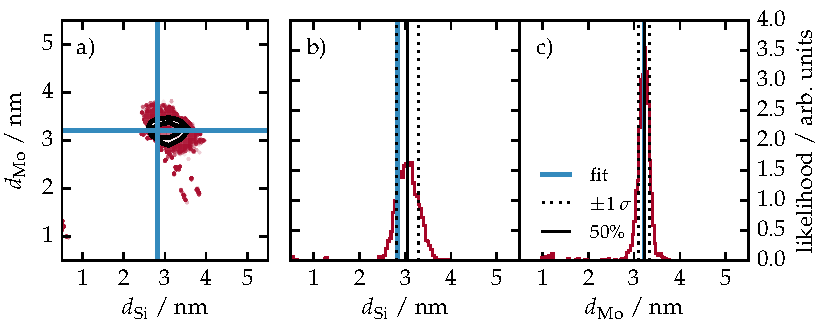
\includegraphics{img/Mo_Si_C_d_Mo_vs_d_Si}
\caption{Results of the maximum likelihood estimation obtained via the \gls{mcmc} procedure similar to Fig.~\ref{ch_spec:fig_ptb17_MCMC_d_Mo_vs_d_Si} but for the combination of \gls{euv} and \gls{xrr} data. a) Two dimensional projection of the likelihood distribution for the parameter pair $d_\text{Si}$ and $d_\text{Mo}$. The projection was obtained by marginalizing over all other parameters of the model. The black contours indicate the areas for one and two standard deviations (one and two sigma contours). The blue lines in all three sub-figures indicate the best parameter set found with the \gls{pso} method. b) One dimensional projection of the likelihood distribution for the silicon layer thickness $d_\text{Si}$. The solid black line marks the center position ($50\%$ percentile) of the distribution. The dotted lines are the limits of one standard deviation. c) The one dimensional distribution similarly to b) for the molybdenum layer thickness.}
\label{ch_spec:fig_Mo_Si_C_d_Mo_vs_d_Si}
\end{figure*}
In comparison to the analysis based on only \gls{euv} data for the Mo/B$_4$C/Si/C in Fig.~\ref{ch_spec:fig_ptb17_MCMC_d_Mo_vs_d_Si}, the inclusion of additional \gls{xrr} measurements lead to significantly smaller confidence intervals and thus higher accuracy of the reconstruction. The method of combining the analysis of two datasets of \gls{euv} and \gls{xrr} measurements has been previously applied by others \cite{yakunin_combined_2014}, which have come to the same result of a significantly improved model reconstruction. Each of the methods does provide different sensitivity for the different model parameters. As an example, \gls{euv} measurements are sensitive to the Mo and Si layer thicknesses due to the large optical contrast in that spectral range. On the other hand, high accuracy can be expected from the \gls{xrr} measurements with respect to the period thickness parameter $D$.

In a second step, another \gls{mcmc} optimization was performed on a reduced parameter set, fixing the determined molybdenum layer thickness to its optimal value, i.e.~the $50\%$ percentile of its distribution. Finally, the layer thicknesses of the C barrier layer and the MoSi$_2$ interdiffusion layer were fixed to their nominal values of $d_C = d_{\text{MoSi}_2} = 0.5 $ nm. Due to the broad distribution result for the likelihoods of those parameters, this comes without a limitation of the generality for this analysis, since any value is valid within the predefined boundaries. Additionally, this ensures comparability of the models for all samples without constraining the applicability of the model with respect to the data available.

\begin{figure}[htbp]
\centering
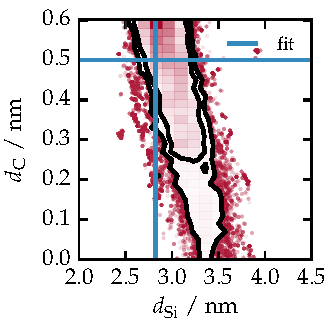
\includegraphics{img/Mo_Si_C_correlation_Si_C}
\caption{Two-dimensional likelihood distribution indicating the correlation of silicon and carbon layer thickness. The distribution was obtained by marginalizing over all remaining parameters of the model. The blue lines indicate the fit obtained through the two-step \gls{mcmc} optimization procedure (see main text).}
\label{ch_spec:fig_Mo_Si_C_correlation_Si_C}
\end{figure}
The results of the second \gls{mcmc} procedure of the restricted model yield the remaining values for the model parameters by obtaining the globally best solution found. The final result is indicated by the blue solid lines in Fig.~\ref{ch_spec:fig_Mo_Si_C_d_Mo_vs_d_Si}. Due to the choice to restrict the model to a buffer layer thickness of $d_\text{C} = \nm{0.5}$, we find the optimal solution for the silicon layer thickness at the limit of one standard deviation in Fig.~\ref{ch_spec:fig_Mo_Si_C_d_Mo_vs_d_Si}b. The distributions shown represent the \gls{mcmc} results of the unrestricted model, where the silicon and carbon layer thicknesses are strongly correlated as shown in Fig.~\ref{ch_spec:fig_Mo_Si_C_correlation_Si_C}. By fixing the carbon layer thickness to its nominal value, this correlation is resolved and the corresponding silicon layer thickness is well within the interval of one standard deviation as indicated through the solid black contours in Fig.~\ref{ch_spec:fig_Mo_Si_C_correlation_Si_C}.

\subsection{Optimization results} \label{ch_spec:sec_mo_si_c_results}
The theoretical reflectivity curves calculated from the optimal model parameters for the unpolished sample with $d_\text{Mo}^\text{nom} = \nm{3.05}$ are shown in Fig.~\ref{ch_spec:fig_EUV_XRR_combined}. Overall, a very good agreement of the two experiments with the theoretical curves is obtained.
\begin{figure}[htbp]
\centering
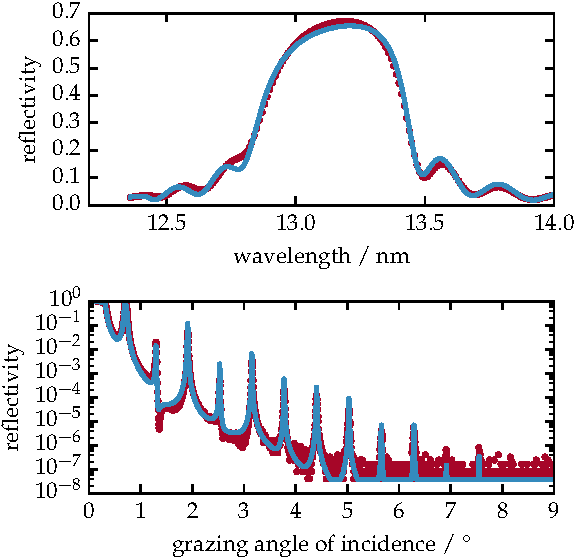
\includegraphics{img/PS5657}
\caption{Experimental data in comparison with the theoretical curves calculated with the model parameters obtained from the combined analysis of \gls{euv} and \gls{xrr} data. The data shown here was measured on the unpolished sample with nominal molybdenum thickness of $d_\text{Mo}^\text{nom} = \nm{3.05}$.}
\label{ch_spec:fig_EUV_XRR_combined}
\end{figure}
The full list for all nominal molybdenum layer thicknesses for all samples with the respective experimental values and their confidence intervals is given in table~\ref{ch_spec:tbl_mo_si_thickness_mcmc_result}.
\begin{table}[htbp]
\centering
\caption{List of nominal molybdenum layer thicknesses in the two sample sets. Both sets were fabricated with a equidistant increase in thickness from \nm{1.70} to \nm{3.05} with 9 unpolished and 10 polished samples.}
\label{ch_spec:tbl_mo_si_thickness_mcmc_result}
\begin{tabular}{@{}lll@{}}
\toprule
nom.~$d_\text{Mo}$ / nm & EUV \& XRR &EUV \& XRR\\ 
&(unpolished) & (polished) \\
\midrule
$1.70$ &$1.81({-0.12}/{+0.24})$  &$1.77({-0.22}/{+0.19})$ \\
$1.85$ &$1.98({-0.15}/{+0.14})$  &$1.91({-0.12}/{+0.17})$ \\
$2.00$ &$2.08({-0.11}/{+0.22})$  &$2.29({-0.28}/{+0.13})$ \\
$2.15$ &$2.31({-0.22}/{+0.21})$  &$2.45({-0.43}/{+0.06})$ \\
$2.30$ &$2.43({-0.09}/{+0.16})$   &$2.60({-0.12}/{+0.14})$ \\
$2.45$ &$2.68({-0.13}/{+0.16})$  &$2.58({-0.21}/{+0.15})$ \\
$2.60$ &$2.91({-0.17}/{+0.12})$ &$2.87({-0.22}/{+0.12})$ \\
$2.75$ &$3.02({-0.15}/{+0.15})$  &$3.03({-0.16}/{+0.14})$ \\
$2.90$ &$3.22({-0.13}/{+0.11})$ &$3.15({-0.13}/{+0.13})$ \\
$3.05$ &-  & $3.47({-0.19}/{+0.13})$ \\
 \bottomrule
\end{tabular}
\end{table}

The optimal parameters for the molybdenum layer thickness $d_\text{Mo}$ and the period thickness $D$ found for both sample sets in the two-step \gls{mcmc} analysis are shown in Fig.~\ref{ch_spec:fig_MoSi_fitted_mo_and_fitted_D}.
\begin{figure*}[htbp]
\centering
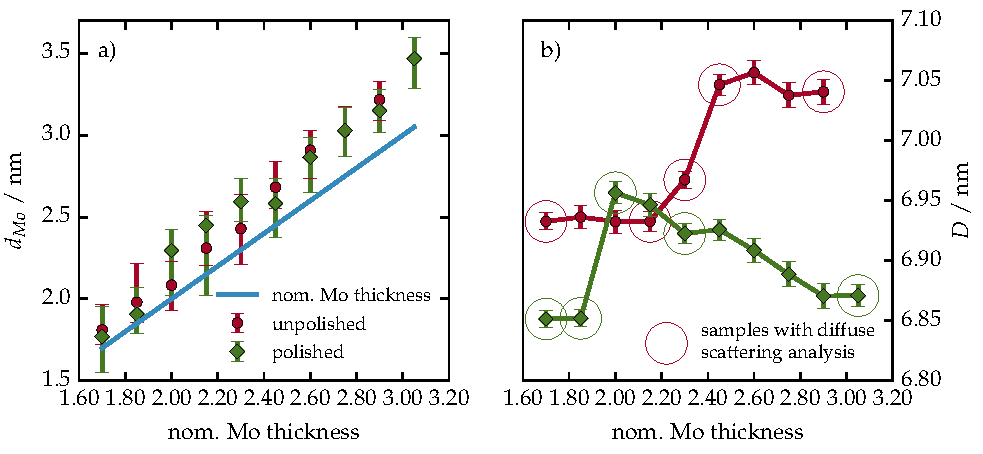
\includegraphics[width=\textwidth]{img/fitted_mo_and_fitted_D}
\caption{a) Fitted Mo thickness values for both sample sets resulting from the MCMC analysis (see text). The nominal Mo layer thickness is shown in comparison in good agreement with the obtained thicknesses. b) Fitted total period thickness $D$ for both sample sets. For both sample sets, clear jumps can be observed at approx.~$d^\text{nom}_\text{Mo} =2.00$ nm and $d^\text{nom}_\text{Mo} =2.38$ nm, respectively, which is attributed to the crystallization threshold (see text). The marked (circle) samples were measured and analyzed with respect to the diffuse scattering.}
\label{ch_spec:fig_MoSi_fitted_mo_and_fitted_D}
\end{figure*}
The confidence intervals shown in Fig.~\ref{ch_spec:fig_MoSi_fitted_mo_and_fitted_D}a are one standard deviation of the likelihood determined for the Mo layer thickness by the first-step MCMC procedure, i.e.~for the unresticted model with the parameter limits as listed in table~\ref{ch_spec:tbl_mo_si_c_multilayer_parameters}. The results show the desired linear increase in molybdenum layer thickness, however at a systematically higher thickness than the nominal values. A possible cause for that observation, consistent with the model reconstruction results, is the possible interdiffusion of the molybdenum layer with the silicon and carbon during deposition and a lower molybdenum density. The reduced relative density of the molybdenum layer is indeed found in the reconstruction results for all samples showing systematically reduced density values of $\rho_\text{Mo} \approx 90\%$ w.r.t.~the Mo bulk density. It is reasonable to assume, that the magnetron sputtered Mo layer, which is in mostly amorphous or polycrystalline state, leads to density reduced layers compared to fully crystalline bulk molybdenum. Thus, the nominal amount of deposited molybdenum leads to higher thicknesses than desired. In Fig.~\ref{ch_spec:fig_MoSi_fitted_mo_and_fitted_D}b the fitted period thicknesses $D$ are shown in dependency of the fitted molybdenum thicknesses.

For both sets, distinct jumps can be observed between $d_\text{Mo}\approx\nm{1.9}$ and $d_\text{Mo}\approx\nm{2.3}$ for the polished samples and between $d_\text{Mo}\approx\nm{2.3}$ and $d_\text{Mo}\approx\nm{2.7}$ for the unpolished set. To better understand this observation, Fig.~\ref{ch_spec:fig_EUV_peak_refl} shows the maximum peak reflectance of all \gls{euv} measurements as a function of the reconstructed Mo layer thickness.
\begin{figure}[htbp]
\centering
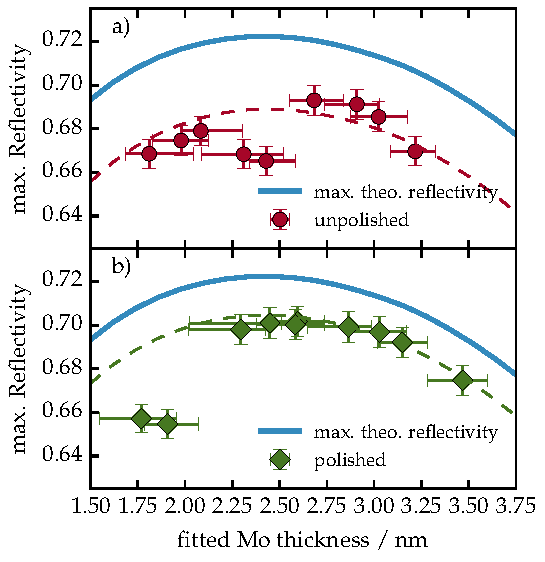
\includegraphics[width=0.6\textwidth]{img/MoSi_EUV_peak}
\caption{Peak reflectance values for each sample obtained from the \gls{euv} measurements for the unpolished sample set (a) and the polished sample set (b). The maximum theoretical reflectance is shown in both subfigures for a perfect (no roughness or interdiffusion) layer system with the same specifications as the samples.}
\label{ch_spec:fig_EUV_peak_refl}
\end{figure}
The identical blue solid line in both subfigures indicates the maximum peak reflectance attainable for a perfect multilayer system with the respective Mo layer thickness without any interdiffusion or roughness. For the calculation, a carbon capping layer of $d_\text{C(cap)} = 2.0$ nm and a relative density of $\rho_\text{C(cap)} = 0.5$ and a silicon dioxide layer of $d_\text{SiO$_2$} = 2.0$ was considered. The dashed curves in both figures show the expected maximum peak reflectance values for the two sample systems calculated by adding the respective roughness/interdiffusion to the model and varying the molybdenum thickness accordingly. In both cases, a significant dip with respect to the expected value can be observed starting at thicknesses of $d_\text{Mo} = 2.31({-0.22}/{+0.21})$ nm for the unpolished samples in Fig.~\ref{ch_spec:fig_EUV_peak_refl}a and at $d_\text{Mo} = 1.77({-0.22}/{+0.19})$ nm for the polished samples in Fig.~\ref{ch_spec:fig_EUV_peak_refl}b. We attribute this significantly diminished peak reflectance to the process of crystallization as the most likely cause. These values are consistent with the increase observed in the period thickness for both cases. Possibly, the deposition is affected by the crystallization threshold causing the increase in period thickness. The values measured here for the dip in peak reflectance are in agreement with earlier observation of molybdenum crystallization in literature \cite{bajt_investigation_2001} for the unpolished sample set. The polishing process shifts that threshold to lower thicknesses by approximately \nm{0.2} to \nm{0.3}.

For a deeper investigation of the interface morphology at the presumed crystallization threshold, \gls{euv} diffuse scattering experiments have been conducted for selected samples of the respective set. To gain a deeper understanding of the reflectivity dip and the period increase, the samples in vicinity of this feature in the Fig.~\ref{ch_spec:fig_EUV_peak_refl} and Fig.~\ref{ch_spec:fig_MoSi_fitted_mo_and_fitted_D} were investigated in comparison to reference samples above and below the threshold. The selection is marked with open circles in Fig.~\ref{ch_spec:fig_MoSi_fitted_mo_and_fitted_D}. This analysis is the topic of chapter~\ref{ch_diff} of this thesis and is described and discussed in detail there based on the model parameters obtained here.

 





\section{Analysis of Cr/Sc Multilayers with Sub-nanometer Layer Thickness}
In the previous sections we have characterized multilayer systems specifically designed to reflect radiation in the \gls{euv} spectral range from \nm{12.5} to \nm{14.0} wavelength. There, the three to four layer systems per period with period thicknesses of $D\approx\nm{7}$ were used to achieve constructive interference at the desired reflection angles. We shall now expand the analysis to a different system. Multilayer mirrors designed to reflect radiation in the spectral range between \nm{2.2} and \nm{4.4} wavelength, the so called \emph{water window}. Those systems share the basic principle of a one-dimensional Bragg crystal with the Mo/Si multilayer stacks from the previous sections, but differ in the selection of materials. The intrinsic relationship between spectral range and period thickness to achieve constructive interference, requires period thicknesses of $D\approx \nm{1.5}$ for this case and higher period replication.


The system we focus on in the rest of this chapter is composed out of a bilayer stack of chromium (Cr) and scandium (Sc). A detailed description of the sample preparation process and the choice of the layer materials can be found in Ch.~\ref{ch_exp}, Sec.~\ref{ch_exp:sec_multilayer_design}. The sample is optimized to reflect radiation of $\lambda = \nm{3.14}$ at an angle of incidence of $\alpha_i = \SI{1.5}{\degree}$. Its periodicity is $N=400$ bilayer periods, where the last period has a larger Cr capping layer thickness. The model of the sample is shown in Fig.~\ref{ch_spec:fig_Cr_Sc_model}.
\begin{figure}[htbp]
    \def\svgwidth{0.7\textwidth}
    \fontfamily{fds}\selectfont\footnotesize
    \import{svg/}{cr_sc_model.pdf_tex}
    \caption{Model of the multilayer stack including the substrate and the capping layers. The periodic part is enclosed between the dashed lines with four layers in each period repeated $N=64$ times. The capping period does not include an interdiffusion layer but has a natural SiO$_2$ layer.}
    \label{ch_spec:fig_Cr_Sc_model}
\end{figure}
The small period thickness of only $D\approx\nm{1.5}$ for this type of sample yields individual layer thicknesses in the sub-nanometer regime, for a bilayer period with approximately equal individual layer thicknesses. This is a significant difference to the Mo/Si systems treated in the beginning of this chapter, where the molybedum and silicon layers were well above $>\nm{1.7}$, even in the smallest case existed. The buffer and interdiffusion layers, which nominally have thicknesses in the same order of magnitude as expected for the Cr/Sc system, could not be characterized based on the methods employed above. We shall therefore first compare the results obtained with an approach similar to the methods in the previous sections to establish a limit to the applicability of discrete layer models.

\subsection{Reconstruction with a discrete layer model approach} \label{ch_spec:sec_CrSc_resconstrution_binary}
In analogy to Sec.~\ref{ch_spec:sec_mo_si_c}, we seek to reconstruct the individual layer thicknesses based on experimental data. For this we construct a discrete layer model as illustrated in Fig.~\ref{ch_spec:fig_Cr_Sc_model} in analogy to the procedure applied for the Mo/Si multilayer systems. The parameters of this discrete layer model are listed in table~\ref{ch_spec:tbl_cr_sc_binary_parameters} together with the upper and lower bound for the particle swarm optimization procedure.
\begin{table*}[htbp]
\centering
\caption{Parametrization of the Cr/Sc binary multilayer model.}
\label{ch_spec:tbl_cr_sc_binary_parameters}
\begin{tabular}{@{}llll@{}}
\toprule
Parameter & Definition & Lower bound & Upper bound\\ \midrule
$d_\text{Cr}$ / nm & Cr layer thickness & $0.0$& $1.5$\\ 
$d_\text{Sc}$ / nm & Sc layer thickness& $0.0$& $1.5$\\ 
$\sigma$ / nm & N\'{e}vot-Croce parameter& $0.0$& $0.5$\\ 
&(identical for all interfaces)&&\\
$\rho_\text{Cr}$ &Cr density w.r.t.~bulk density & $0.5$& $1.0$\\ 
$\rho_\text{SC}$ &Sc density w.r.t.~bulk density& $0.5$& $1.0$\\ 
\midrule
\multicolumn{4}{c}{Capping layer}\\
\midrule
$d_\text{C (cap)}$ / nm & C capping layer thickness & $0.0$&$1.0$ \\ 
$d_\text{CrO (cap)}$ / nm & SiO$_2$ capping layer thickness & $0.0$&$1.5$ \\ 
$d_\text{Cr (cap)}$ / nm & SiO$_2$ capping layer thickness & $0.0$&$3.0$ \\ 
$\rho_\text{C (cap)}$ &C density w.r.t.~bulk density& $0.0$& $1.0$\\ 
$\rho_\text{CrO (cap)}$& CrO density w.r.t.~bulk density& $0.0$& $1.0$\\
$\rho_\text{Cr (cap)}$& Cr (cap) density w.r.t.~bulk density & $0.5$& $1.0$  \\
 \bottomrule
\end{tabular}
\end{table*}

The reflectivity of the sample in the water window spectral range from \nm{3.12} to \nm{3.16} was measured at the \gls{sx700} beamline at \gls{bessy}. The angle of incidence was $\alpha_i=\SI{1.5}{\degree}$ (corresponding to a grazing angle of incidence of $\alpha_i^\text{GI} = \SI{88.5}{\degree}$), which corresponds to the design goal for this mirror prototype. In addition, similar to the Mo/Si samples, a \gls{xrr} measurement was 
conducted in the DESY laboratory using a laboratory-based X-ray diffractometer 
(X'Pert PRO MRD, Panalytical). The diffractometer is equipped with a high-resolution goniometer and uses Cu-K$_\alpha$ radiation as a source. The \gls{xrr} intensities were recorded using a PIXcel counting detector. The dynamic range achieved in the measurements 
extended down to a reflectance of $10^{-6}$ for grazing angles of incidence of 
$\alpha_i=0^\circ$ to $\alpha_i=3^\circ$.

Both measurement curves are shown together in Fig.~\ref{ch_spec:fig_CrSc_EUV_XRR_data}.
\begin{figure}[htbp]
  \centering
  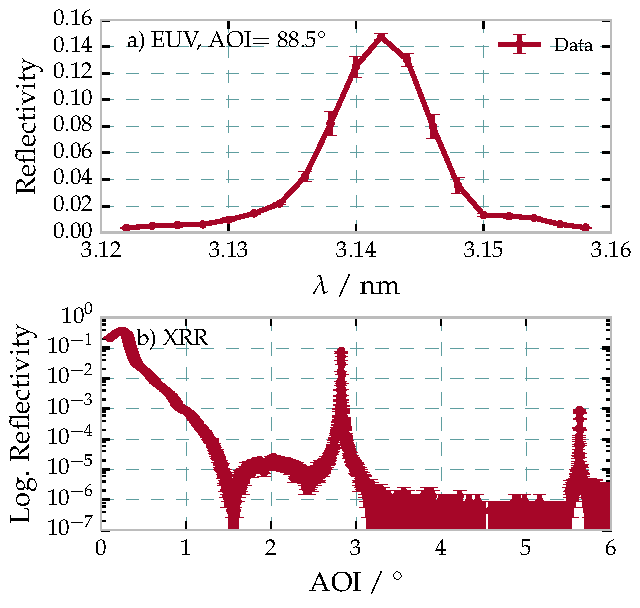
\includegraphics[width=0.6\textwidth]{img/CrSc_EUV_XRR_data}
  \caption{\Gls{euv} and \gls{xrr} data recorded for the Cr/Sc sample system. a) The \gls{euv} curve was obtained at an angle of incidence $\alpha_i=\SI{1.5}{\degree}$. b) The \gls{xrr} curve was recorded using a Cu-K$_\alpha$ source with a photon energy of $E_\text{ph}=\ev{8048}$.}
  \label{ch_spec:fig_CrSc_EUV_XRR_data}
\end{figure}
Due to the short period of the multilayer sample, only two Bragg peaks could be observed in this angular range in the \gls{xrr} curve. All expected higher order peaks were below the detection threshold of $10^{-6}$ in reflected intensity. The dominating experimental uncertainty was the inhomogenity of the sample stack across the sample area. The given uncertainty values for each of the measurement points were estimated, by measuring the peak reflectance of the \gls{euv} reflectivity curve on positions marking a cross of \mm{2} by \mm{2} in the sample center. This data was compared to theoretical expectance value based on a \gls{pso} fit of the discrete layer model above (for details of the optimization results see below). From this a drift of the period thickness of $D=\SI{2}{\pico\meter}$ was obtained and uncertainties were calculated as the difference of two theoretical curves attaining the maximum and minimum $D$ values. Similarly, uncertainties for the \gls{xrr} curve was calculated by simulating theoretical curves based on the same period drifts.

In comparison, the most remarkable difference with respect to the Mo/Si mirrors is the significantly reduced peak reflectance of the \gls{euv} curve in Fig.~\ref{ch_spec:fig_CrSc_EUV_XRR_data}a compared to the curves in Fig.~\ref{ch_spec:fig_ptb17_reflectance_AOI_15} and Fig.~\ref{ch_spec:fig_EUV_reflectivity_unpolished_and_polished_with_peak_refl}c. The maximum experimental value attained is only approximately $R_\text{max} \approx 15\%$ while it is up to $R_\text{max} \approx \SI{70}{\percent}$ for the Mo/Si systems. The reasons for this are the different spectral range and the material properties at the water window wavelengths.

To better illustrate the differences to the Mo/Si systems, we have conducted an 
analysis based on the discrete layer model of a Cr/Sc multilayer as described above. The particle swarm optimization was done based on the EUV data shown in Fig.~\ref{ch_spec:fig_CrSc_EUV_XRR_data}a and the parameters and limits listed in table~\ref{ch_spec:tbl_cr_sc_binary_parameters}. The resulting parameters are listed in table~\ref{ch_spec:tbl_cr_sc_binary_pso_results}.
\begin{table}[htbp]
\centering
\caption{\gls{pso} fit results for the discrete layer Cr/Sc multilayer model.}
\label{ch_spec:tbl_cr_sc_binary_pso_results}
\begin{tabular}{@{}ll@{}}
\toprule
Parameter &  \gls{pso} result\\ \midrule
$d_\text{Cr}$ / nm &  $0.8224$\\ 
$d_\text{Sc}$ / nm &  $0.7510$\\ 
$\sigma$ / nm &  $0.375$\\ 
$\rho_\text{Cr}$  & $0.876$\\ 
$\rho_\text{Sc}$ & $0.957$\\ 
\midrule
\multicolumn{2}{c}{Capping layer}\\
\midrule
$d_\text{C (cap)}$ / nm  & $0.462$ \\ 
$d_\text{CrO (cap)}$ / nm  & $1.143$ \\ 
$d_\text{Cr (cap)}$ / nm  & $2.322$ \\ 
$\rho_\text{C (cap)}$ & $0.502$\\ 
$\rho_\text{CrO (cap)}$& $0.618$\\
$\rho_\text{Cr (cap)}$ & $0.851$\\
 \bottomrule
\end{tabular}
\end{table}
The capping layer results were obtained in a combined \gls{pso} analysis based on the \gls{euv} and \gls{xrr} data excluding the areas of the Bragg peaks. This grazing incidence reflectivity data has a very high sensitivity for the top surface layers, which can not be deducted from an \gls{euv} curve alone as demonstrated in Sec.~\ref{ch_spec:sec_reconstruction_PTB17}.

The theoretical curve obtained from the \gls{pso} procedure is shown in Fig.~\ref{ch_spec:fig_CrSc_binary_fit_vs_max_refl} in direct comparison with the theoretically achievable maximum reflectivity curve.
\begin{figure}[htbp]
  \centering
  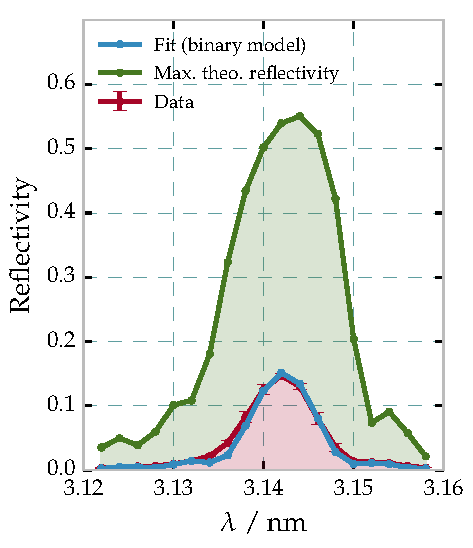
\includegraphics[width=0.45\textwidth]{img/CrSc_binary_fit_vs_max_refl}
  \caption{Fitted experimental EUV reflectance curves across the wavelength 
of the radiation impinging at $\alpha_i=1.5^\circ$ from normal, based on the binary 
model. The green curve shows the maximum theoretical reflectance assuming a perfect multilayer system without roughness or interdiffusion.}
  \label{ch_spec:fig_CrSc_binary_fit_vs_max_refl}
\end{figure}
The latter was obtained by calculating the resulting reflectivity based on the parameter results in table~\ref{ch_spec:tbl_cr_sc_binary_pso_results}, but without any roughness or interdiffusion, i.e.~by requiring $\sigma \equiv 0.0$. The Sc 
to Cr ratio was found to be $\Gamma_\text{Sc}= d_\text{Sc}/d_\text{Cr} = 0.48$ with a \gls{rms} value of $\sigma=0.385$ nm for the N\'{e}vot-Croce factor. While the EUV reflectance curve shows excellent agreement with the measured data, there is a significant offset to the theoretically achievable maximum reflectance. For the particular model derived above, theoretical reflectance values of $R_\text{max} > \SI{50}{\percent}$ are possible. This large difference, especially compared to Mo/Si systems which are very close to the theoretically achievable maximum reflectance (cf.~Fig.~\ref{ch_spec:fig_EUV_peak_refl}), hints at strong roughness or intermixing of the two materials. To verify the applicability of the discrete (binary) layer model used here, the calculated curves for both experiments, the \gls{euv} and \gls{xrr} curve, are shown together in Fig.~\ref{ch_spec:fig_CrSc_binary_model_EUV_vs_XRR}.
\begin{figure*}[htbp]
  \centering
  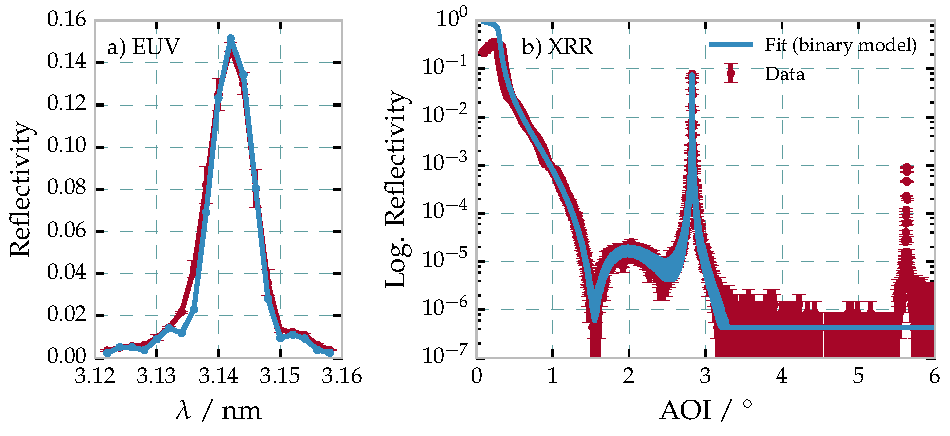
\includegraphics[width=\textwidth]{img/CrSc_binary_model_EUV_vs_XRR}
  \caption{a) Measured \gls{euv} reflectivity curve for the near-normal angle of incidence of $\alpha_i=\SI{1.5}{\degree}$ together with the theoretical curve based on the \gls{pso} optimized binary multilayer model. b) Measured and calculated \gls{xrr} curves for the same sample and model parameters at grazing angles of incidence using radiation at the Cu-K$_\alpha$ wavelength. A clear mismatch of the theoretical curve and the measured data can be observed for the second Bragg peak between $\alpha_i^\text{GI} = \SI{5.0}{\degree}$ and $\alpha_i^\text{GI} = \SI{6.0}{\degree}$.}
  \label{ch_spec:fig_CrSc_binary_model_EUV_vs_XRR}
\end{figure*}

Again, the \gls{euv} data is matched excellently, while in the case of the \gls{xrr} measurement the first Bragg peak is found to be matched by the model also in the X-ray regime. However, the second Bragg resonance, clearly visible with a peak reflectance value of approximately $10^{-3}$ is not represented by the model at all. A fully
combined analysis similarly to the approach in Sec.~\ref{ch_spec:sec_mo_si_c} could not yield a consistent result. The \gls{rms} value for $\sigma$ required to reduce the theoretical EUV reflectance down to the measured 
level could not be brought into agreement with the second Bragg peaks in the \gls{xrr} curve. In a strictly binary model like this one with a layer thickness ratio of 
$\Gamma_\text{Sc}\approx 0.5$, the second Bragg peak is additionally suppressed 
due to symmetry reasons. Thus, there is a clear mismatch of the model reconstruction and the experimental observations, mostly due to the complementary data delivered through the measurement of the second Bragg peak of the \gls{xrr} curve. This is a strong indicator, that the simple model as defined above does not suffice to describe the physical situation of the sample. Therefore, a more elaborate model is required introducing additional parameters to account for the increased complexity of the samples layer properties compared to the Mo/Si sample systems above.

\subsection{Extending The Model to Graded Interfaces and Interdiffusion} \label{ch_spec:sec_CrSc_gradual_model}
The physical situation of Cr/Sc multilayer systems with individual layer thicknesses in the sub-nanometer regime is significantly different than in comparably large thicknesses of several nanometers such as in the Mo/Si case of the two preceding sections. It is well known \cite{prasciolu_thermal_2014}, that magnetron sputtered Cr and Sc multilayer systems, similarly to the Mo/Si systems, suffer from imperfect interfaces. The main reason for that is interdiffusion of the two materials into each other. In addition, roughness at the interfaces exists and further diminishes an ideal chemically abrupt transition from one material to the next. Due to the small layer thicknesses required to achieve the first Bragg resonance upon near-normal incidence with radiation of $\lambda=\nm{3.14}$, roughness and interdiffusion may occur over an interdiffusion zone as large as the total layer thickness itself. The results from the specular \gls{euv} and \gls{xrr} measurements shown above, clearly demonstrate that a binary model with only a N\'{e}vot-Croce damping parameter $\sigma$ due not provide an accurate model for the physical reality. Instead, a more complex model is required. Here, we define a periodic model, repeated in units of one bilayer period, to account for possible interdiffusion gradients and intermixing between the two materials in the stack. The symmetry of two identically thick layers within one period in the simple model above leads to a suppression of the second order Bragg peak. Nevertheless, physically this symmetry effect can be broken by accounting for interdiffusion zones with different thicknesses, depending on whether Cr was deposited on Sc or vice versa. Thereby, the second Bragg peak is no longer suppressed even though both layers have the same thickness if the interdiffusion zones are asymmetric. Physical causality further dictates, that the two layers intermix gradually. The model, which we use to reconstruct the Cr/Sc multliayer sample measured above is illustrated in Fig.~\ref{ch_spec:fig_CrScModel} in direct comparison to the simple model used before.
\begin{figure*}[htb]
    \def\svgwidth{\textwidth}
    \import{svg/}{CrSc_model.pdf_tex}
    \caption[Binary and gradual Cr/Sc multilayer models.]{a) Binary Cr/Sc multilayer model with total period thickness $D$ and 
the individual layer thicknesses $d_\text{Sc}$ and $d_\text{Cr}$. b) Model with 
explicit gradual interfaces following a sinusoidal profile. The ideal interface 
profile is approximated through discrete sublayers as indicated in red, forming 
the actual gradual interface profile entering the electric field calculations. 
The thickness of the interdiffusion zones can differ for the top and bottom 
interface in each period. Their total thicknesses are given by $s_\text{Sc}$ 
and $s_\text{Cr}$. The effective index of refraction for both layers is given 
by $\tilde{n}_\text{Sc}$ and $\tilde{n}_\text{Cr}$, respectively.}
    \label{ch_spec:fig_CrScModel}
\end{figure*}
The interdiffsion zones are modeled following a sinosodial profile, which represents a smooth transition from the refractive index of the Cr layer to the Sc layer and vice versa. The thickness of those zones is given by the parameters $s_\text{Sc}$ and $s_\text{Cr}$. For the calculation of the electromagnetic fields inside the stack, the interface region is sampled with a fixed number of equally spaced points in $z$-direction, effectively creating a region of thin sublayers with a gradually changing index of refraction (illustrated by the red steped function in Fig.~\ref{ch_spec:fig_CrScModel}). To take into account intermixing extending across the full period, we introduced an intermixing parameter $\eta$. The effective indices of refraction of the individual Cr and Sc layers are then given through
\begin{align}
\tilde{n}_\text{Cr} &=(\eta/2) n_\text{Sc} + (1-\eta/2) n_\text{Cr} \text{,} 
\nonumber\\
\tilde{n}_\text{Sc} &=(1-\eta/2) n_\text{Sc} + (\eta/2) n_\text{Cr} \text{,} 
\label{eqn:effective_n} \\
&\text{for} \quad \eta \in [0,1] \text{,}\nonumber
\end{align}
where $n_\text{Cr}$ and $n_\text{Sc}$ are the tabulated values \cite{henke_x-ray_1993} 
with densities $\rho_\text{Cr}$ and $\rho_\text{Sc}$.

With the definition of the model as outlined above, natural restrictions arise for the parameters. As an example, the interdiffusion zone region can not extend across half of the thickness of the original layers total thickness described by the parameter $d_\text{Cr}$ or $d_\text{Sc}$, respectively. Instead, the intermixing parameter would have to be increased to account for that situation. The model is therefore parameterized according to the list of effective parameters given in table~\ref{ch_spec:tbl_CrSc_gradual_parametrization} together with their allowed ranges for the optimization procedure in analogy to the analysis conducted in the previous sections. The range limits arise either from physical plausibility or are intrinsic properties of the parameter definition.
\begin{table*}[htbp]
\centering
\caption{Multilayer parametrization and parameter limits}
\label{ch_spec:tbl_CrSc_gradual_parametrization}
\begin{tabular}{@{}llll@{}}
\toprule
Parameter & Definition & Lower bound & Upper bound\\ \midrule
$D$ / nm & $= d_\text{Sc} + d_\text{Cr}$ & 1.5&1.6 \\ 
$\Gamma_{Sc}$ & $= d_\text{Sc} / D$&0.0 &1.0 \\ 
$s_d$ / nm&$=s_\text{Sc} + s_\text{Cr}$&0.0 & 1.6\\ 
$\Gamma_s$ &$= s_\text{Sc} / s_d$& 0.0& 1.0\\ 
$\eta$ &layer intermixing& 0.0& 1.0\\ 
$\sigma_r$ / nm & r.m.s.~roughness& 0.0& 0.5\\ 
$\rho_{Sc}$ &Sc density w.r.t.~bulk density & 0.5& 1.0\\ 
$\rho_{Cr}$ &Cr density w.r.t.~bulk density& 0.5& 1.0\\ 
 \bottomrule
\end{tabular}
\end{table*}
Here, $D$ is the full period thickness, $d_\text{Sc}$ and $d_\text{Cr}$ are the 
nominal layer thicknesses of the Cr and Sc layers as indicated in 
Fig.~\ref{ch_spec:fig_CrScModel}, and $\rho_\text{Sc}$ and $\rho_\text{Cr}$ their 
respective densities with respect to their bulk densities 
$\tilde{\rho_\text{Sc}} = 2.989$ g/cm$^3$ and $\tilde{\rho_\text{Cr}} = 7.19$ 
g/cm$^3$ \cite{henke_x-ray_1993}. The loss of specular 
reflectance due to roughness-induced scattering is considered through the 
N\'{e}vot-Croce factor using $\sigma_\text{r}$ identical at each interface. This is necessary to account for diffusely scattered light, which is missing in the measured specularly reflected radiation but can not be attributed to contrast loss due to interdiffusion. The parameter $\Gamma_\text{Sc}$ indicates the portion of the Sc layer thickness 
with respect to the full period thickness $D$, which together uniquely define the thickness $d_\text{Cr}$; $\Gamma_\sigma$ describes the 
asymmetry of the widths of the interdiffusion zones at the Cr on Sc and Sc on Cr 
interfaces and is intrinsically limited to the interval $\Gamma_\sigma \in [0,1]$. Note that 
$s_\text{Sc}$ and $s_\text{Cr}$ are half periods of the sinus functions used to 
describe the interface profiles. Therefore the condition $s_\text{Sc} + 
s_\text{Cr} \leq D$ holds.

The discretization of the smooth interface profile in the interdiffusion zones introduces an additional numerical uncertainty through the number of discretization points $n$ required to reflect the physical situation of a smooth transition. To assert a lower limit for this number, we have evaluated the mean error introduced by coarse sampling. The most accurate experiment of the analysis within this chapter is given by the \gls{euv} reflectivity curve, which serves as a reference for this assertation through the sum of the squared uncertainty of each data point in Fig.~\ref{ch_spec:fig_CrSc_EUV_XRR_data}a, $\sum_m \tilde{\sigma}_m$. 

The numerical error of the model depending on the interface sampling through gradual sublayers was evaluated by comparing the sum of squares
\begin{align}
\chi_n &= \sum\limits_m (I^{n=100}_m - I^n_m)^2
\end{align}
of the difference of the theoretical \gls{euv} curves with increasing numbers of gradual interfaces and an ``ideal'' smooth transition represented by $100$ sublayers. The model parameters used for this analysis were obtained through a \gls{pso} optimization of the model with respect to the \gls{euv} reflectivity curve.
\begin{figure}[htbp]
  \centering
  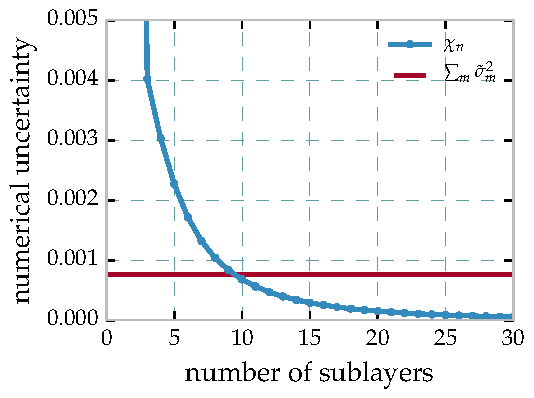
\includegraphics[width=0.45\textwidth]{img/CrSc_numerical_uncertainty_mixlayer}
  \caption{Numerical uncertainty introduced through a coarse graded layer model in comparison with the experimental uncertainty.}
  \label{ch_spec:fig_CrSc_numerical_uncertainty_mixlayer}
\end{figure}
As illustrated in Fig.~\ref{ch_spec:fig_CrSc_numerical_uncertainty_mixlayer}, the experimental uncertainty dominates at the lower limit of $n=10$ sublayers for the interface zone.
For the analysis is this chapter, and due to reasons of numerical efford required to calculate the electromagnetic field for all measurements discussed here, we use $n=15$ sublayers for all calculations. At that value, the experimental uncertainty is clearly dominant and only a marginal additional uncertainty is aquired due to insufficient sampling.

As a verification of the applicability of the model to the problem of accurately representing a physical situation that could describe the \gls{euv} and \gls{xrr} data shown in Fig.~\ref{ch_spec:fig_CrSc_EUV_XRR_data} above, we have applied the combined analysis technique for the two data sets described in Sec.~\ref{ch_spec:sec_MoSi_euv_xrr_combined} to the improved gradual model. The particle swarm optimization approach is applied to obtain a global solution for the model parameters by minimizing the functional defined in Eq.~\eqref{ch_spec:eqn_Mo_Si_C_total_chi_2}. The results found for the binary model (cf.~Fig.~\ref{ch_spec:fig_CrSc_binary_model_EUV_vs_XRR}) and the gradual model are shown in direct comparison with each other in Fig.~\ref{ch_spec:fig_CrSc_bianry_vs_gradual_model_fits}.
\begin{figure*}[htbp]
  \centering
  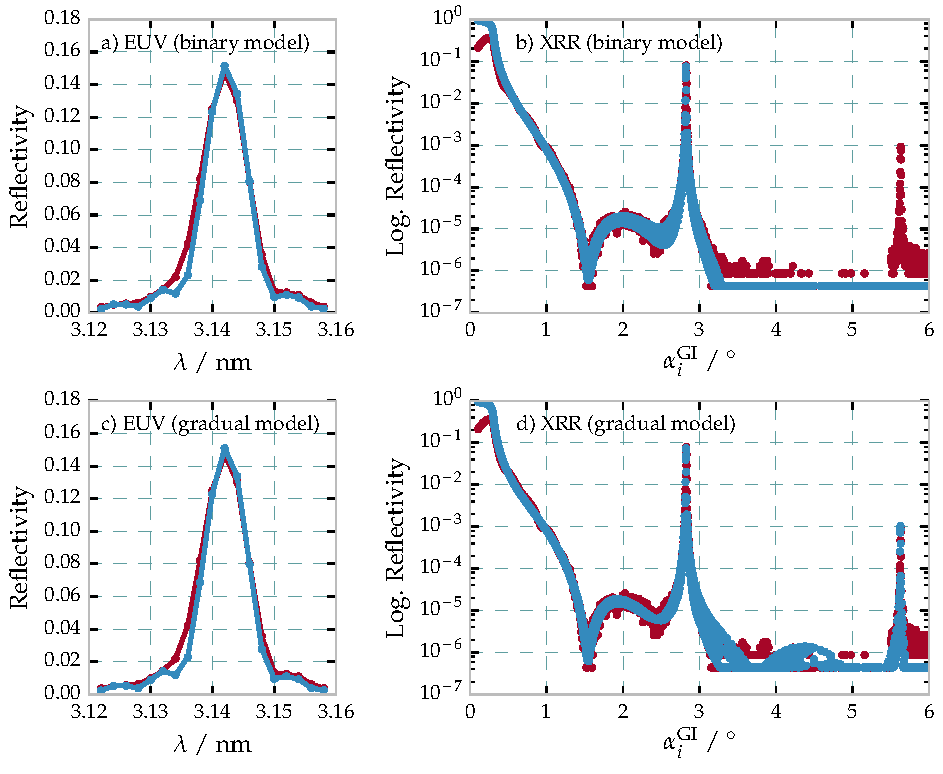
\includegraphics[width=\textwidth]{img/CrSc_bianry_vs_gradual_model_fits}
  \caption{Comparison of the reconstructions of the binary and gradual models for the \gls{euv} and \gls{xrr} data. a) Measured \gls{euv} reflectivity curve for and near-normal angle of incidence of $\alpha_i=\SI{1.5}{\degree}$ together with calculated curve of the \gls{pso}-based binary model reconstruction. b) Measured and calculated \gls{xrr} curves for the same sample and model parameters at grazing angles of incidence using radiation at the Cu-K$_\alpha$ wavelength. A clear mismatch of the theoretical curve and the measured data can be observed for the second Bragg peak between $\alpha_i^\text{GI} = \SI{5.0}{\degree}$ and $\alpha_i^\text{GI} = \SI{6.0}{\degree}$.
  c) Measured \gls{euv} reflectivity curve for and near-normal angle of incidence of $\alpha_i=\SI{1.5}{\degree}$ together with calculated curve of the \gls{pso}-based gradual model reconstruction. d) Measured and calculated \gls{xrr} curves for the same sample and model parameters at grazing angles of incidence using radiation at the Cu-K$_\alpha$ wavelength.}
  \label{ch_spec:fig_CrSc_bianry_vs_gradual_model_fits}
\end{figure*}
The \gls{euv} reflectivity curves show visually indistinguishable fits for both, the binary model as already found above and also the gradual model in Fig.~\ref{ch_spec:fig_CrSc_bianry_vs_gradual_model_fits}a and Fig.~\ref{ch_spec:fig_CrSc_bianry_vs_gradual_model_fits}c. For the binary model, we have seen the distinct mismatch with the second order Bragg peak, which is shown once again in Fig.~\ref{ch_spec:fig_CrSc_bianry_vs_gradual_model_fits}b. For the gradual interface model, we see a significant improvement of the optimized result with perfectly match in both Bragg peaks of the \gls{xrr} curve in Fig.~\ref{ch_spec:fig_CrSc_bianry_vs_gradual_model_fits}d while also maintaining an excellent agreement with the \gls{euv} curve.

Based on the example of a combined analysis of \gls{euv} and \gls{xrr} data in this section, the gradual interface model clearly provides a more accurate representation of the physical reality in the sample than the binary approach by offering a reconstruction satisfying both data sets. At the same time, the results show that a verification of the model only becomes possible by adding complementary information. In case of the example above, that information is provided through the appearance of a second Bragg peak in the \gls{xrr} curve. Thereby, the limiting case of the binary model, which is still possible for the new gradual model, can be excluded with certainty through the comparison shown in Fig.~\ref{ch_spec:fig_CrSc_bianry_vs_gradual_model_fits}. The main difference of both models is the local gradual change of the index of refraction, which attributes for the fact that both materials can intermix. More importantly, both materials can intermix differently with respect to the specific interface, i.e.~the situation where Cr is deposited on top of Sc or vice versa. A key element of obtaining a reconstruction of that particular model is thus the application of techniques, which can deliver information on the spacial distribution of the materials within one period.

At that point, it should be noted that other distortions of a perfect layer system can be imagined, which are not covered by a strictly periodic model as the one introduced above. Those include drifts of the period thickness $D$ across the stack or other systematic aperiodicities. In that case, however, a broadening of the peak or a distortion of the peaks symmetry, most prominently in the \gls{euv} curve, would be observed, which is not the case. Although situations may occur, where the aperiodicities could lead to effects compensated by tuning the parameters of the gradual interface model, this assumption would assume a more complex situation than the simple assumption of periodicity and is thus implausible.
To further strengthen that argument, we shall calculate the distortion occurring through a drift in the depostion process. This is a plausible systematic error, which could be caused by instabilities in the deposition process. Fig.~\ref{ch_spec:fig_CrSc_drift} shows the peak distortion for a drift of the total period thickness $D$ across the whole stack of $N=400$ periods by $d_\text{drift} = \nm{0.005}$ based on the model parameters for the curves in Fig.~\ref{ch_spec:fig_CrSc_bianry_vs_gradual_model_fits}c. Clearly, already this small drift would cause a distortion of the peak symmetry, which is not observed in the data and a drift thus unlikely.
\begin{figure}[htbp]
  \centering
  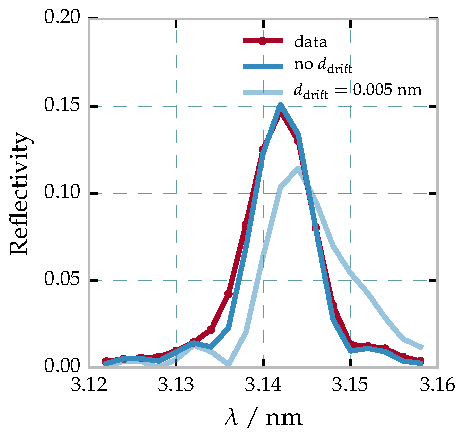
\includegraphics{img/CrSc_drift}
  \caption{\Gls{euv} peak deformation assuming a constant drift of $d_\text{drift} = \nm{0.005}$ across the total multilayer stack.}
  \label{ch_spec:fig_CrSc_drift}
\end{figure}

\subsection{Addition of Complementary Experimental Methods}
Due to the increased complexity of the model, the question arises how accurately any parameter of the model can be determined and whether correlations exist and can be resolved (cf.~Fig.~\ref{ch_spec:fig_Mo_Si_C_correlation_Si_C} as an example for correlated model parameters in case of Mo/Si multilayer systems) based on the available data and whether further analytical measurements can improve the result as this was clearly the result for the \gls{euv} and \gls{xrr} experiments shown above. For the particular case of the gradual interface model for periodic multilayer systems with sub-nanometer layer thicknesses, in total four experiments were conducted to study the applicability of each method with respect to finding a unequivocal reconstruction including confidence intervals. Only by systematically analyzing the strength and weaknesses of the employed analytic methods, a reconstruction of the model resembling the reality inside the sample becomes possible.

\subsubsection{Resonant EUV Reflectivity}
As seen for the four layer system discussed in Sec.~\ref{ch_spec:sec_reconstruction_PTB17}, confidence intervals for the individual layer thicknesses in the range below \nm{1} could not be obtained by exclusively analyzing the \gls{euv} curve. Similarly, the combined analysis of \gls{euv} and \gls{xrr} experiments in Sec.~\ref{ch_spec:sec_MoSi_euv_xrr_combined} did improve the result but still shows fairly large confidence intervals concerning the small total layer thickness in the Cr/Sc systems. For the particular system discussed here with possibly strong interdiffusion, a technique is required that yields the total amount of Sc and equivalently Cr within a single period. For that purpose, resonant reflectivity experiments in the \gls{euv} spectral range are promising. The knowledge of the optical constants are a necessary requirement for deducting quantitative information from that kind of experiment. In case of Sc, those were measured precisely for the Sc L3 and L2 absorption edges at approximately $\lambda_\text{Sc-L} \approx \nm{3.1}$ and below by \textcite{aquila_measurements_2004}. The real and imaginary parts obtained from that experiments are shown together with the respective optical constants of Cr in Fig.~\ref{ch_exp:fig_crsc_contrast} of Sec.~\ref{ch_exp:sec_multilayer_design} in  Ch.~\ref{ch_exp}. To exploit the information contained in the optical constants of Sc, angular resolved reflectivity curves across the first Bragg peak were recorded at several wavelengths across the Sc L-edge. As the Cr dispersion is changing only marginally and smoothly across that wavelength range, any change of contrast and absorption can be attributed to the Sc in the multilayer. The corresponding measurements are shown in Fig.~\ref{ch_spec:fig_CrSc_REUV_data}.
\begin{figure}[htbp]
  \centering
  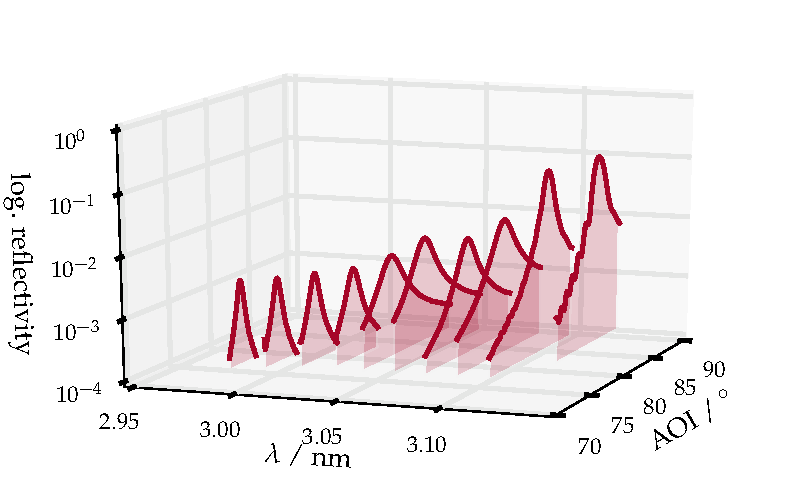
\includegraphics[width=0.7\textwidth]{img/CrSc_REUV_data}
  \caption{Measured resonant \gls{euv} reflectivity curves across the Sc L2 and L3-edge in logarithmic representation. At each equidistant photon energy point, an angular resolved reflectivity curve was recorded across the Bragg peak.}
  \label{ch_spec:fig_CrSc_REUV_data}
\end{figure}
Each reflectivity curve was recorded within the interval from $\alpha_i = \SI{2.5}{\degree}$ to $\alpha_i = \SI{19.0}{\degree}$, depending on the selected wavelength. The wavelength range was chosen between $\lambda = \nm{2.986}$ and $\lambda = \nm{3.128}$ including the Sc L2 and L3 edges. The resulting data is analyzed in analogy to the \gls{euv} reflectivity curves in Sec.~\ref{ch_spec:sec_CrSc_gradual_model} by applying the matrix algorithm on basis of the gradual layer model and the optical constants by \textcite{aquila_measurements_2004}. The experimental uncertainties taken into account for the \gls{reuv} experiment were estimated on basis of the multilayer inhomogenity deducted as described for the \gls{euv} experiment in Sec.~\ref{ch_spec:sec_CrSc_resconstrution_binary}. The details of the reconstruction based on this dataset are shown below in this section.

\subsubsection{Grazing Incidence X-ray Fluorescence}
In addition to the reconstruction of the Sc content via the \gls{reuv} experiment, spacial resolved measurements are necessary to deduct the interface profile in the gradual layer model. As discussed in Sec.~\ref{ch_spec:sec_CrSc_gradual_model}, asymmetric interface regions provide a possibility to observe a second Bragg peak in the \gls{xrr} measurement, even though both layers in the period have equal nominal thickness. To obtain information on that spacial distribution of both materials within a period, \gls{xrf} experiments exploiting the formation of a standing wave when scanning across the first Bragg peak were performed. The details of the method and how spacial sensitivity can be obtained are described in detail in Ch.~\ref{ch_theo}, Sec.~\ref{ch_theo:sec_xrf}.

The sample was measured exciting fluorescence of the Sc and Cr K-lines, which show the highest fluorescence yield for the core shell transitions. The K-edges for both materials are at energies of $E_\text{Sc-K} = \ev{4492}$ and $E_\text{Cr-K} = \ev{5989}$ \cite{elam_new_2002}. The experiment was therefore conducted at the \gls{fcm} beamline at \gls{bessy} in grazing incidence geometry at photon energies of $E_\text{ph} = \ev{5500}$ and $E_\text{ph} = \ev{6250}$, well above the respective edges as described in Ch.~\ref{ch_exp}, Sec.~\ref{ch_exp:sec_xrf_at_fcm}. Depending on which energy was used, the Bragg peak is found at grazing angles of incidence of $\alpha_i^\text{GI} \approx \SI{4.12}{\degree}$ and $\alpha_i^\text{GI} \approx \SI{3.62}{\degree}$, respectively. The measured relative fluorescence yield in the vicinity of the first Bragg peak is shown in Fig.~\ref{ch_spec:fig_CrSc_fluorescence_data} for both photon energies and materials.
\begin{figure*}[htbp]
  \centering
  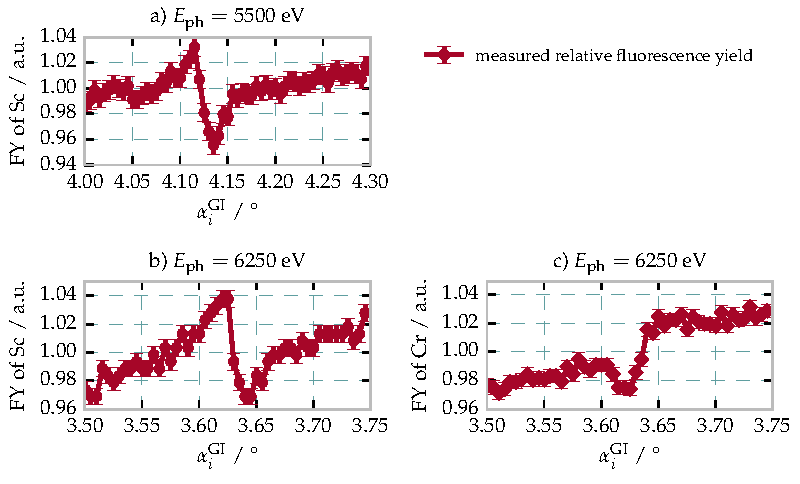
\includegraphics[width=\textwidth]{img/CrSc_fluorescence_data}
  \caption{Measured relative X-ray fluorescence curves for the Cr and Sc K-lines across the first Bragg peak. a) Relative fluorescence yield of the Sc K-line at a primary photon energy of $E_\text{ph}=\ev{5500}$. b), c) Relative fluorescence yield for both materials at an primary photon energy of $E_\text{ph} = \ev{6250}$.}
  \label{ch_spec:fig_CrSc_fluorescence_data}
\end{figure*}
Since the photon energy of $E_\text{ph} = \ev{5500}$ is below the K-edge of Cr, only data for the Sc K-fluorescence exists. In the second case, fluorescence from both materials was detected. The measurement uncertainties were estimated from the distribution of the data for regions away from the Bragg resonance.

The fluorescence curves for Cr and Sc show distinctly different behavior, of the expected curve shape (cf.~Fig.~\ref{ch_theo:fig_xrf_scheme}). For the analysis, the result at photon energies of $E_\text{ph}=\ev{5500}$ (Fig.~\ref{ch_spec:fig_CrSc_fluorescence_data}a)  was not taken into account, as the information is redundant to the result at  $E_\text{ph}=\ev{6250}$ (Fig.~\ref{ch_spec:fig_CrSc_fluorescence_data}b). As mentioned above, the theoretical description on how the relative fluorescence is calculated based on the gradual model is elaborated on in detail in Ch.~\ref{ch_exp}, Sec.~\ref{ch_exp:sec_xrf_at_fcm}.

\subsection{Reconstruction and Maximum Likelihood Evaluation}
With the two additional measurements described above, the total of four data sets (\gls{euv}, \gls{xrr}, \gls{reuv} and \gls{xrf}) are available for the Cr/Sc multilayer sample to reconstruct the parameters of the gradual interface model. The full dataset is compiled in Fig.~\ref{ch_spec:fig_CrSc_all_data}.
\begin{figure*}[htbp]
  \centering
  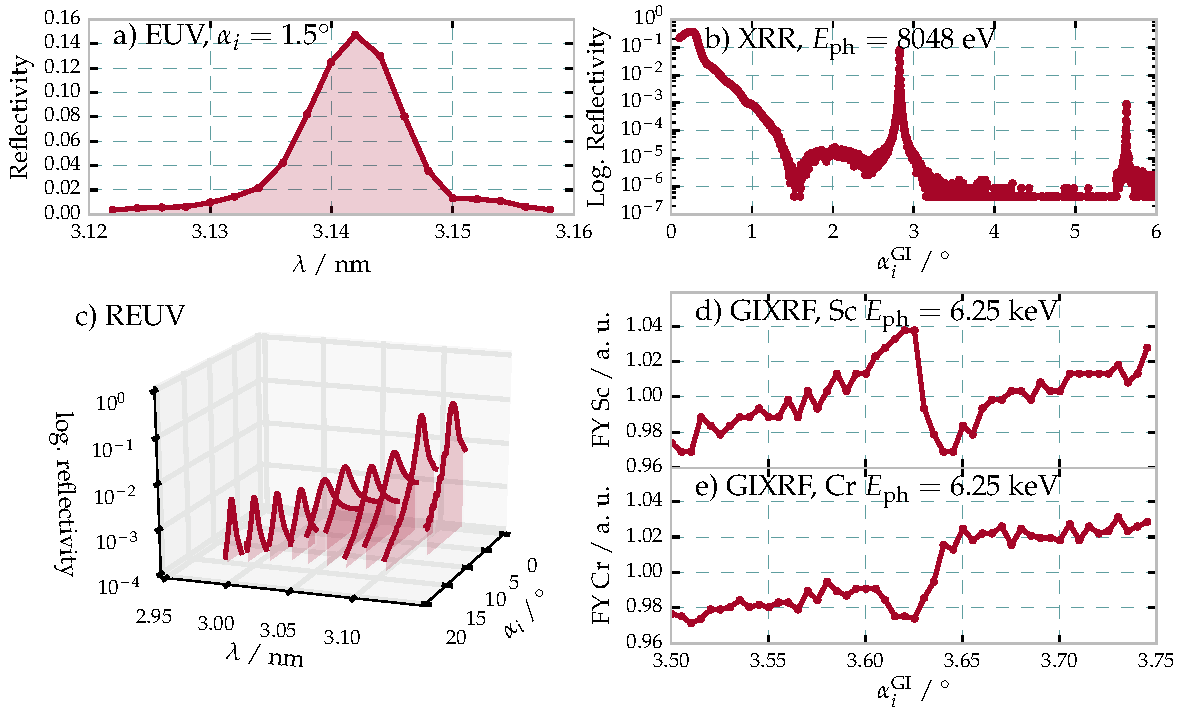
\includegraphics[width=\textwidth]{img/CrSc_all_data}
  \caption{Full data set used in the combined analysis. Due to redundancy, the \gls{xrf} data for the Sc at a photon energy of $E_\text{ph}=\ev{5500}$ was omitted.}
  \label{ch_spec:fig_CrSc_all_data}
\end{figure*}

As in the combined analysis conducted for the Mo/Si/C systems in Sec.~\ref{ch_spec:sec_MoSi_euv_xrr_combined}, we define the minimization functional for the combined analysis of all the datasets as
\begin{align}
\chi^2 = \tilde{\chi}^2_\text{EUV} +\tilde{\chi}^2_\text{XRR} 
+\tilde{\chi}^2_\text{REUV} + 
\tilde{\chi}^2_\text{GIXRF(Sc)}+\tilde{\chi}^2_\text{GIXRF(Cr)}\text{,} 
\label{ch_spec:eqn_CrSc_total_chi_2}
\end{align}
where each of the reduced functionals is defined as
\begin{align}
\tilde{\chi}^2 = \frac{1}{M - P} \bigg[\sum\limits_{m} \frac{(I_m^\text{model} 
- I_m^\text{meas})^2}{\tilde{\sigma}_m^2} \bigg] \text{,} 
\label{ch_spec:eqn_CrSc_reduced_chi_2}
\end{align}
with $M$ being the number of measurement points in each experiment and $P$ the 
number of parameters for the model. Statistical and systematic uncertainties 
for each data point are included in $\tilde{\sigma}_m$. The definition of 
Eq.~\eqref{ch_spec:eqn_CrSc_total_chi_2} ensures that all experiments are weighted equally 
considering their respective uncertainties. This functional corresponds to the combined $\chi^2$ functional defined in \eqref{ch_spec:eqn_Mo_Si_C_total_chi_2}, augmented by the additional measurements conducted here.

Firstly, similar as for the other two sample systems treated in this chapter, the parameters of the model, here the gradual interface model with the parameters and their limits listed in table~\ref{ch_spec:tbl_CrSc_gradual_parametrization}, were obtained using the \gls{pso} method to find a solution reproducing the experimental results. Secondly, following the maximum likelihood approach employing the \gls{mcmc} method as detailed in Sec.~\ref{ch_spec:sec_maximum_likelihood}, starting from this the uniqueness and confidence intervals for each parameter were obtained. The \gls{pso} result was further refined by taking the $50\%$ percentile of the resulting likelihood distribution for each parameter.

Through the minimization of the combined $\chi^2$ functional in Eq.~\eqref{ch_spec:eqn_CrSc_total_chi_2} via the \gls{pso} method, the best model parameters were obtained. It should be noted here, that in case of the \gls{xrr} curve, the analyzed data set was restricted to the two visible Bragg peaks which contain the information on the periodic part of the layer system. The data in between those does reflect the top surface layer thicknesses and was therefore analyzed separately to obtain the capping layer thicknesses after the optimization of the periodic part. The results for the capping layer thicknesses listed in table~\ref{ch_spec:tbl_CrSc_best_model_capping} was consequently used throughout the theoretical analysis for all experiments described here.
\begin{table}[htbp]
\centering
\caption{Optimized model parameters obtained by \gls{pso} analysis}
\label{ch_spec:tbl_CrSc_best_model_capping}
\begin{tabular}{@{}ll@{}}
\toprule
Parameter &  \gls{xrr} (areas in between the peaks)\\ \midrule
$d_\text{C (cap)}$ / nm  & $0.709$ \\ 
$d_\text{CrO (cap)}$ / nm  & $0.913$ \\ 
$d_\text{Cr (cap)}$ / nm  & $ 2.495$ \\ 
$\rho_\text{C (cap)}$ & $0.527$\\ 
$\rho_\text{CrO (cap)}$& $0.548$\\
$\rho_\text{Cr (cap)}$ & $0.791$\\
 \bottomrule
\end{tabular}
\end{table}

\subsubsection{Confidence Intervals and Evaluation of the Experimental Methods}
As discussed numerously throughout this chapter, the single optimization based on an \gls{pso} result ideally delivers a global minimum of the respective optimization functional. However, no information is obtained about the uniqueness and accuracy of the solution or correlation of parameters causing ambiguity of the results. Consequently, in addition to fitting the data with a particle swarm optimizer, each result was verified based on the \gls{mcmc} method described above to evaluate the confidence intervals for each parameter. To assess the performance of each of the experimental methods individually, the two step process, i.e.~the \gls{pso} fitting procedure followed by the \gls{mcmc} sampling, was conducted for each standalone experiment as well as for the combined optimization problem stated in Eq.~\eqref{ch_spec:eqn_CrSc_total_chi_2}.

The results are compiled in Table \ref{ch_spec:tbl_CrSc_MCMC_results}. The confidence intervals were calculated by evaluating the probability distribution as a result of the \gls{mcmc} procedure for each parameter around its \gls{pso} fit results. The confidence intervals given here represent percentiles of the number of samples found in the interval defined by the upper and lower bounds used for the \gls{pso} procedure for each parameter. In the case of 
a centered Gaussian distribution, percentiles of $2.3\%$ and $97.8\%$ of the integrated number of samples forming the distribution, mark the interval of four times the standard deviation, i.e.~$\pm 2\sigma$ in statistical terms. Due to potential asymmetries in the actual distributions found by the \gls{mcmc} method, explicit upper and lower bounds of the confidence intervals are given in table \ref{ch_spec:tbl_CrSc_MCMC_results} based on these percentiles. The best model value is based on the \gls{pso} fit result and is refined by the \gls{mcmc} sampling by calculating the mean value, i.e.~the 50\% percentile, of the distribution of samples following the \gls{mcmc} procedure.
\begin{table*}
\centering
\caption{Optimized model parameters with confidence intervals derived from MCMC 
validation for each individual experiment and the combined analysis}
\label{ch_spec:tbl_CrSc_MCMC_results}
\begin{tabular}{@{}llllll@{}}
\toprule
Parameter &  Combined & EUV  & XRR  & REUV  & GIXRF\\ \midrule
$D$ / nm& $1.5737_{-0.0010}^{+0.0008}$ & $1.5749_{-0.0022}^{+0.0014}$ & 
$1.5726_{-0.0042}^{+0.0035}$& $1.5728_{-0.0019}^{+0.0016}$& 
$1.5741_{-0.0024}^{+0.0021}$ \\ \addlinespace
$\Gamma_{Sc}$ & $0.48_{-0.04}^{+0.04}$ & $0.35_{-0.11}^{+0.14}$ & 
$0.42_{-0.26}^{+0.35}$& $0.52_{-0.07}^{+0.09}$& $0.49_{-0.10}^{+0.09}$ \\ 
\addlinespace
$s_d$ / nm& $1.34_{-0.26}^{+0.18}$ & $0.72_{-0.66}^{+0.67}$ & 
$0.60_{-0.57}^{+0.78}$& $0.89_{-0.83}^{+0.59}$& $1.27_{-0.38}^{+0.24}$ \\ 
\addlinespace
$\Gamma_\sigma$ & $0.16_{-0.16}^{+0.51}$ & $0.29_{-0.28}^{+0.64}$ & 
$0.40_{-0.39}^{+0.57}$& $0.33_{-0.32}^{+0.61}$& $0.39_{-0.37}^{+0.57}$ \\ 
\addlinespace
$\eta$ & $0.56_{-0.16}^{+0.06}$ & $0.44_{-0.30}^{+0.16}$ & 
$0.38_{-0.36}^{+0.33}$& $0.52_{-0.37}^{+0.14}$& $0.37_{-0.34}^{+0.25}$ \\ 
\addlinespace
$\sigma_r$ / nm& $0.11_{-0.10}^{+0.11}$ & $0.17_{-0.15}^{+0.12}$ & 
$0.13_{-0.12}^{+0.14}$& $0.17_{-0.16}^{+0.16}$& $0.27_{-0.25}^{+0.20}$ \\ 
\addlinespace
$\rho_{Sc}$ & $0.94_{-0.12}^{+0.05}$ & $0.84_{-0.32}^{+0.15}$ & 
$0.78_{-0.27}^{+0.21}$& $0.94_{-0.14}^{+0.06}$& $0.83_{-0.30}^{+0.17}$ \\ 
\addlinespace
$\rho_{Cr}$ & $0.98_{-0.08}^{+0.02}$ & $0.96_{-0.13}^{+0.04}$ & 
$0.83_{-0.27}^{+0.16}$& $0.90_{-0.21}^{+0.09}$& $0.86_{-0.28}^{+0.14}$ \\ 
\addlinespace
 \bottomrule
\end{tabular}
\end{table*}

\begin{figure*}[htbp]
  \centering
  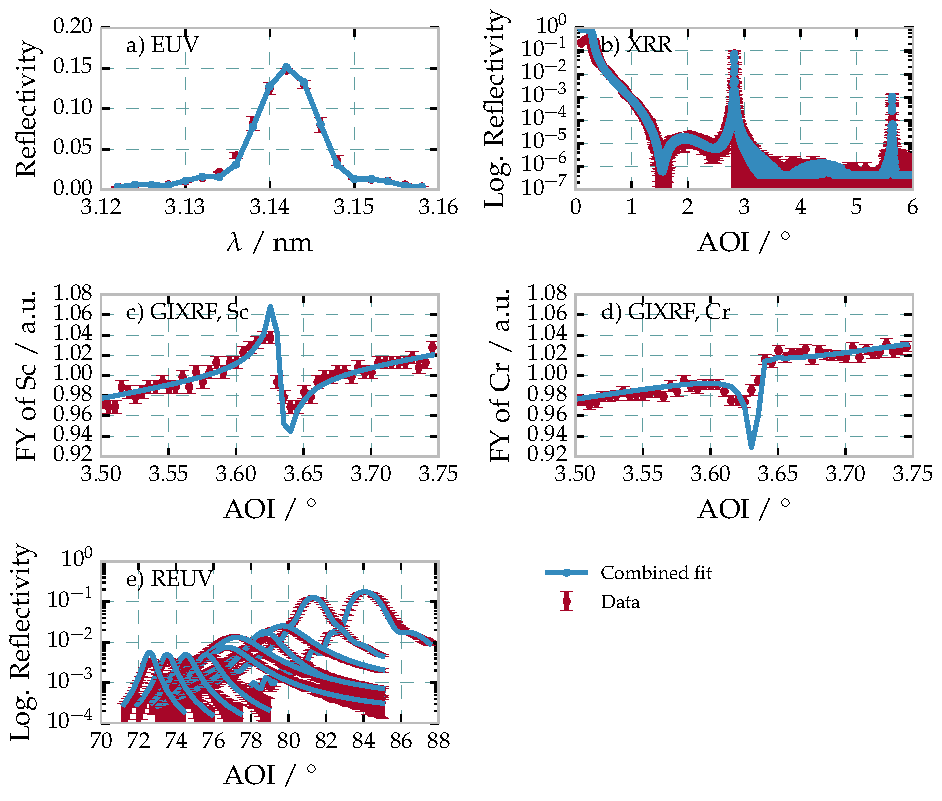
\includegraphics[width=\textwidth]{img/CrSc_combined_fit_result}
  \caption{Measured reflectance and fluorescence yield curves in direct comparison with the calculated reflectance and intensity curves for the 
optimized parameters obtained through the combined analysis of all experiments as listed in 
table~\ref{ch_spec:tbl_CrSc_MCMC_results}.}
  \label{ch_spec:fig_combined_fit_result}
\end{figure*}
Before discussing the achieved reconstruction and the corresponding confidence intervals of each of the methods in detail, we shall view the theoretical curves calculated from the best model of the combined analysis. The curves are shown in direct comparison with the data from Fig.~\ref{ch_spec:fig_CrSc_all_data} including the respective experimental uncertainties in Fig.~\ref{ch_spec:fig_combined_fit_result}. Clearly, the data and the solution found in the optimization procedure show excellent agreement indicating that the gradual interface model indeed provides a very good representation of physical reality with respect to the experiments conducted here. Nevertheless, differences can be observed. The reason lies 
in the fact that the model is potentially still too ideal. Small variations 
during the deposition process, for example, could lead to imperfections, which 
are not described in a strictly periodic model. However, including these by 
explicitly breaking the periodicity would again lead to an ill-defined model 
with a vastly increased number of parameters and is thus not practical. Another 
reason is the deviation in the homogeneity of the sample, e.g.~a varying period 
across the sample, which cause mismatches if the measurement position varies 
slightly between the different experimental setups. The latter effects were 
considered in the uncertainties of the individual measurements by measuring the 
EUV reflectivity at positions $\pm 2$ mm from the center position and fitting 
the model. The result was a $\Delta D = 2$ pm shift in the period over $4$ mm 
across the sample.


\paragraph{Parameter correlations in the combined analysis}
With the optimized model parameters listed in table~\ref{ch_spec:tbl_CrSc_MCMC_results} and shown in Fig.~\ref{ch_spec:fig_combined_fit_result} for the combined analysis, a model reconstruction could be obtained explaining the data for each of the experiments. The \gls{mcmc} sampling of the likelihood functional based on the $\chi^2$ definition in Eq.~\eqref{ch_spec:eqn_CrSc_total_chi_2} yields the corresponding confidence intervals for all parameters and experiments given through the upper and lower bound as described above. Here, we shall illustrate and discuss in detail the resulting likelihood distributions obtained from the combined analysis, as they show that correlations of the parameters could be resolved and only persist for a single important case. For that, Fig.~\ref{ch_spec:fig_CrSc_cornerplot_combined} shows the full matrix of two- and one-dimensional likelihood distribution projections marginalizing over all other parameters. The details of how this figure is to be interpreted are described in detail above in Sec.~\ref{ch_spec:sec_maximum_likelihood} for the example of Mo and Si layer thicknesses obtained through fitting \gls{euv} reflectivity data.
\begin{figure*}[htbp]
  \centering
  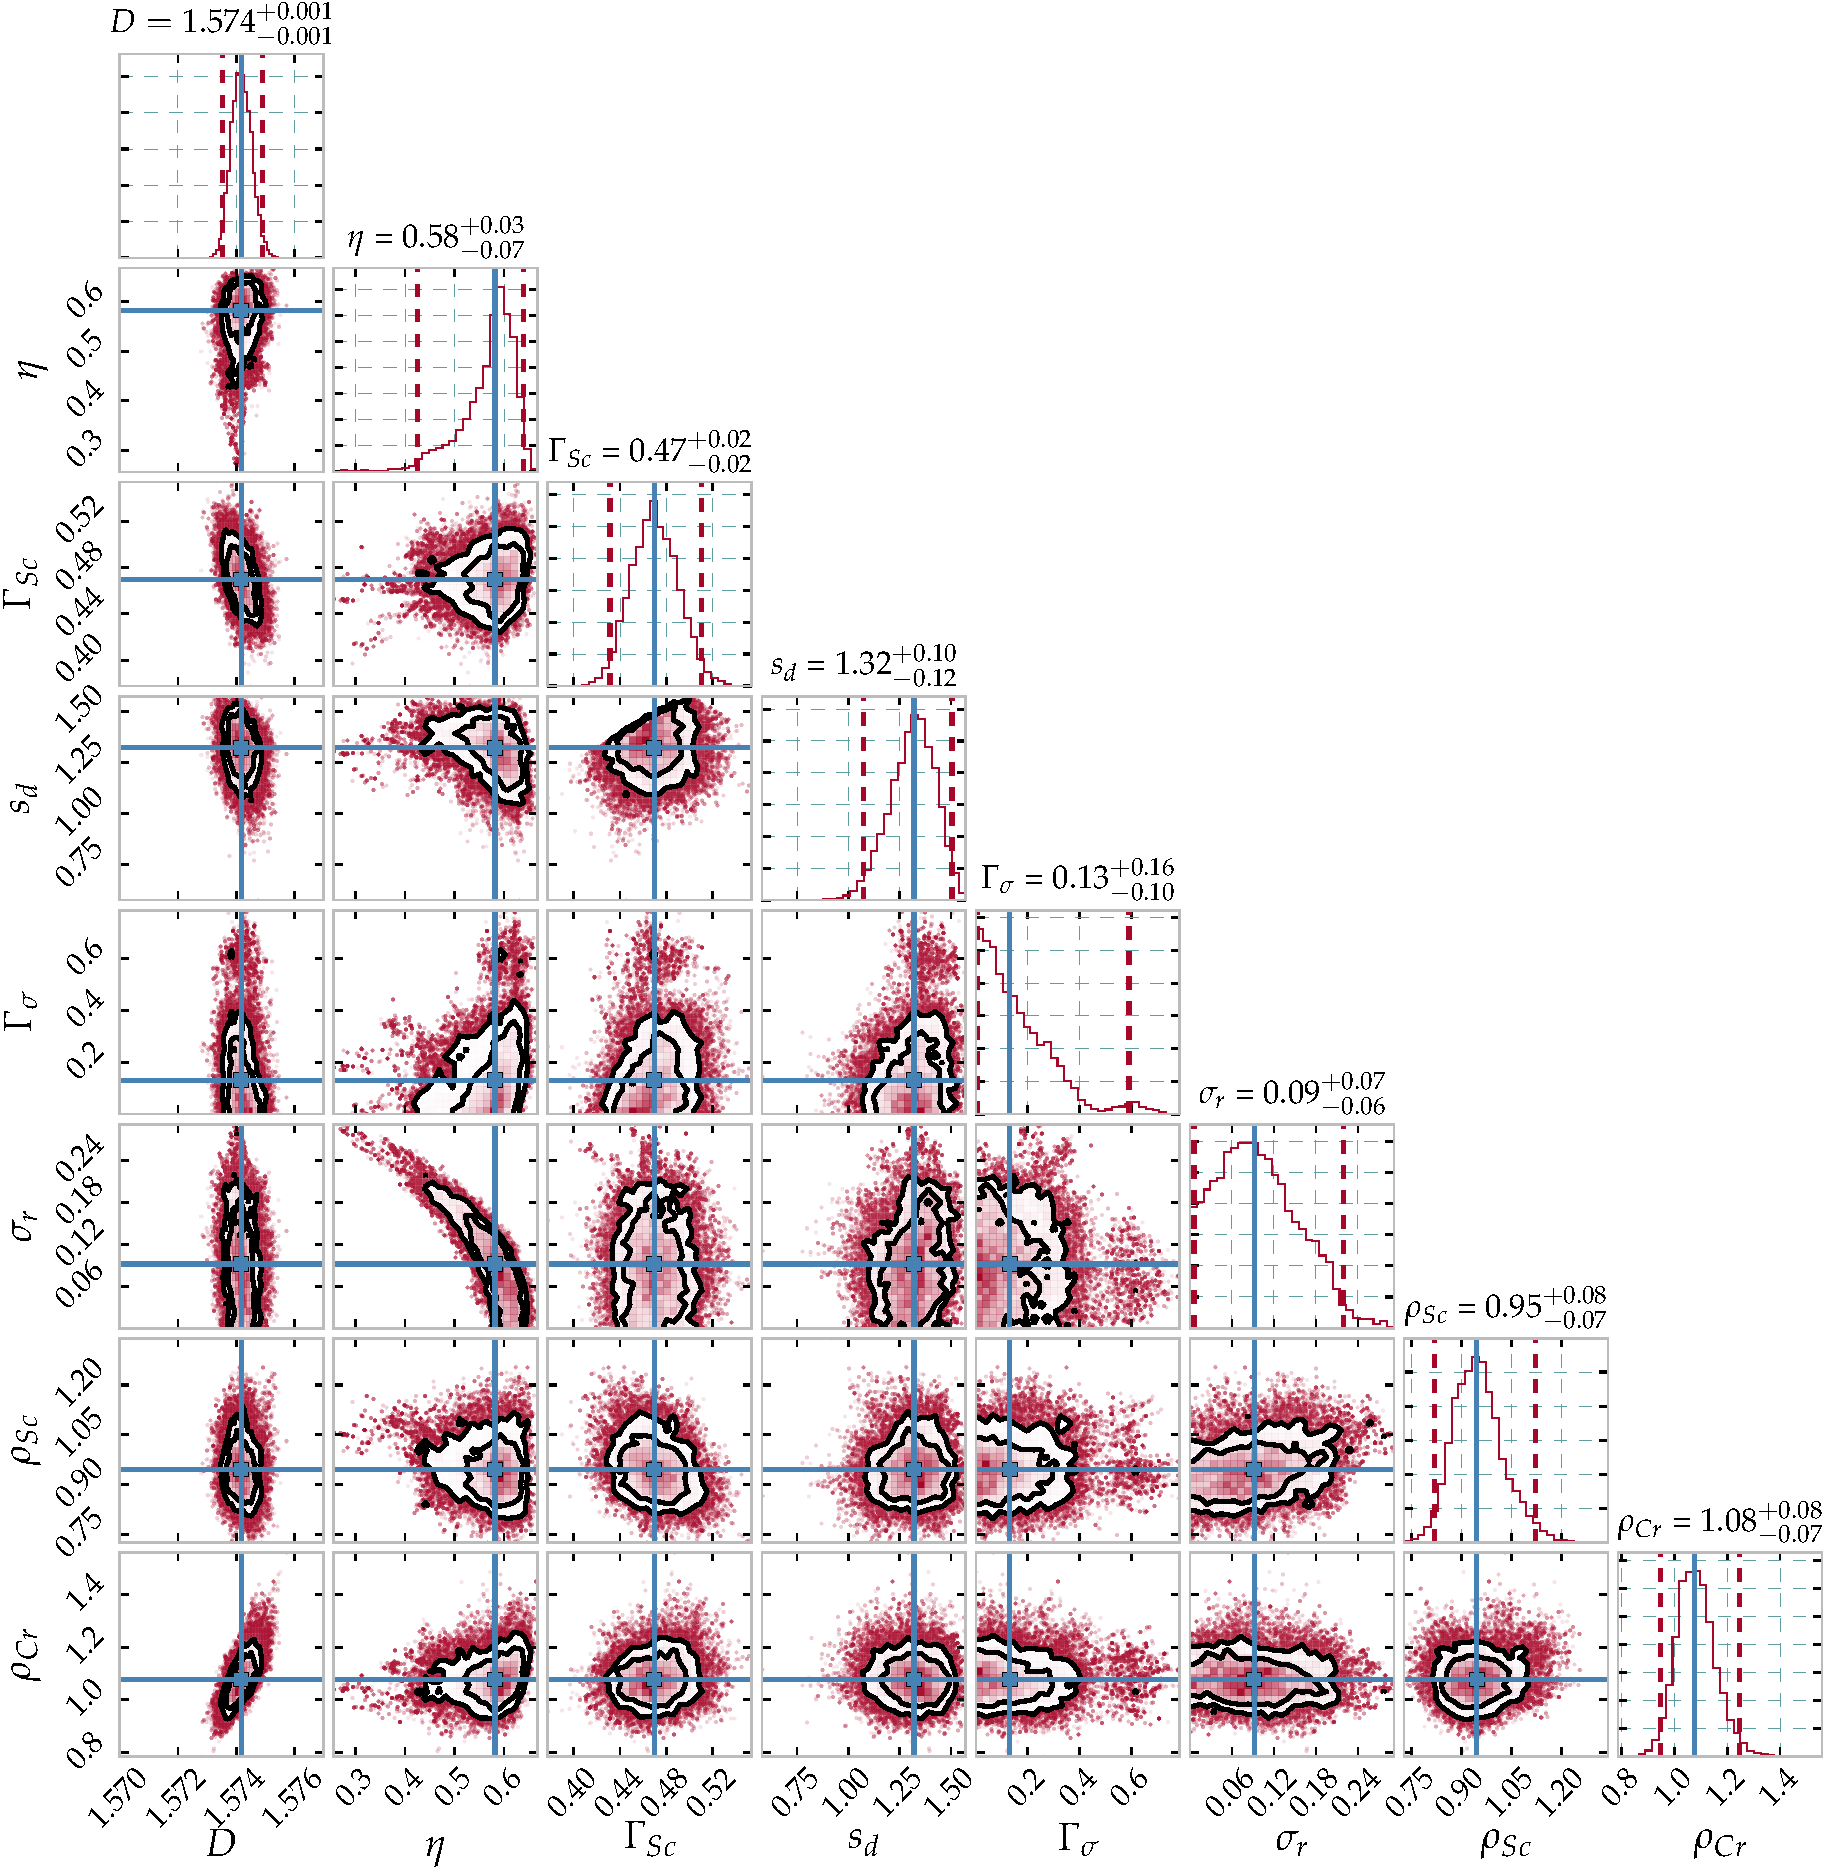
\includegraphics[width=\textwidth]{img/CrSc_cornerplot_combined}
  \caption{Matrix representation of the result of the maximum likelihood analysis based on the \gls{mcmc} method for all parameter combinations. At the top of each column, the one-dimensional projection of the likelihood distribution for the respective parameter is shown in analogy to the figures \ref{ch_spec:fig_Mo_Si_C_d_Mo_vs_d_Si} or \ref{ch_spec:fig_ptb17_MCMC_other_params}. The dotted red lines indicate the $\pm 2 \sigma$ interval, i.e.~two standard deviations from the center value ($\SI{50}{\percent}$ percentile). The latter is indicated through the solid blue lines. In the two dimensional projections, the solid black contours mark the areas for one and two standard deviations, respectively. For a discussion of the observed features see main text}
  \label{ch_spec:fig_CrSc_cornerplot_combined}
\end{figure*}
Here, all possible gradual interface model parameter combinations are shown as two dimensional histograms together with the one-dimensional projection at the diagonal of the plot matrix. The solid blue line represents the values of the optimized model after both, the \gls{pso} and refining through the \gls{mcmc} method. They correspond to the values listed in table~\ref{ch_spec:tbl_CrSc_MCMC_results} for the combined analysis column.

Generally, most of the parameter combinations do not show distinct correlations but approach the shape of a two-dimensional Gaussian distribution, which would be expected for a unique solution with corresponding uncertainty. It should be noted that in some cases, the distribution is truncated by parameter limits, which follow from physical or mathematical restrictions on the parameters as discussed in Sec.~\ref{ch_spec:sec_CrSc_gradual_model}, such as for the densities $\rho_\text{Sc}$ and $\rho_\text{Cr}$ as well as for the interface region ratio $\Gamma_\sigma$. In addition, the latter parameter shows a bimodal distribution for all two-dimensional histograms with clear emphasis on the lower value. That is a particularly interesting result of the combined analysis as it clearly demonstrates that only strongly asymmetric interface regions are minimizing the $\chi^2$ functional and it may thus be concluded that this corresponds to the physical reality in the sample.

Finally, the parameter set of the \gls{rms} roughness $\sigma_r$ and the interdiffusion parameter $\eta$ show a ``banana shaped'' correlation significantly broadening the confidence intervals for both parameters. Fig.~\ref{ch_spec:fig_CrSc_eta_rho_correlation} shows a magnification of that particular histogram to better illustrate this property.
\begin{figure}[htbp]
  \centering
  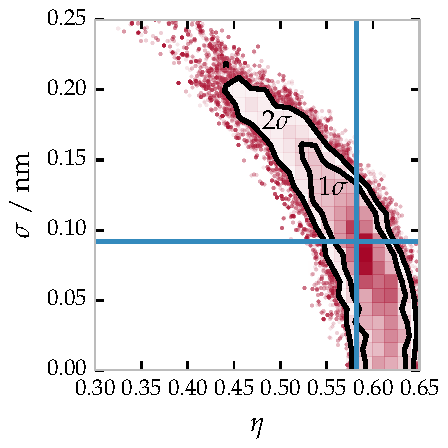
\includegraphics{img/CrSc_eta_rho_correlation}
  \caption{Magnified two dimensional projection histogram for the correlation of the interdiffusion parameter $\eta$ and the \gls{rms} roughness parameter $\sigma_r$ from Fig.~\ref{ch_spec:fig_CrSc_cornerplot_combined}. Again, the areas of one and two standard deviations are indicated together with the $\SI{50}{\percent}$ percentile as solid blue lines.}
  \label{ch_spec:fig_CrSc_eta_rho_correlation}
\end{figure}
The broad spectrum of values covered by the distribution in both parameters hints at a indistinguishability of those two model parameters, and consequently physical properties of the sample, based on the analyzed data. In fact, this conclusion can easily be understood as none of the applied experimental methods can separate the effect of roughness and interdiffusion. For better understanding this, we shall consider the relatively large beam footprint, with the smallest one of all experiments covering and area of approximately \mm{1} by \mm{1}, in comparison to the roughness dimensions and frequencies expected in the order of nanometers. Thereby, any reflected radiation or fluorescence radiation excited within the multilayer always represents an average of the rough interface morphology. That, however, can not be distinguished from a homogeneous layer with gradual interdiffusion along the surface normal of the sample. The solution to this problem of distinction is the analysis of diffuse scattering from the sample in addition to the combined analysis, which is the topic of the Ch.~\ref{ch_diff} of this thesis.

\paragraph{Confidence intervals depending on the employed method}
The confidence intervals of each experimental method differ significantly as table~\ref{ch_spec:tbl_CrSc_MCMC_results} shows. The reason behind this is the different sensitivity of the methods to the specific physical properties described by the respective model parameter. To better illustrate the information compiled in the table above, for each method and each parameter the total confidence interval is shown in Fig.~\ref{fig:confidence_intervals} in a radial plot. The total confidence interval is defined as the difference of the upper and lower values as listed in table~\ref{ch_spec:tbl_CrSc_MCMC_results} for each experiment and parameter.
\begin{figure}[htbp]
  \centering
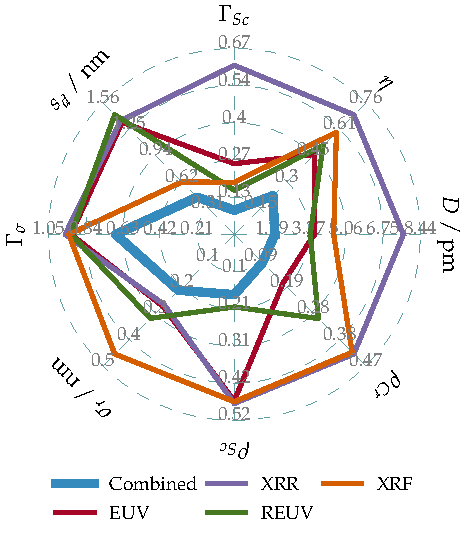
\includegraphics{img/CrSc_confidence_intervals_radar}
  \caption{Visual representation of the total confidence intervals for each of 
the parameters with respect to each of the individual experiments as well as 
the combined analysis.}
  \label{fig:confidence_intervals}
\end{figure}
The plot shows the four relevant experiments and the combined analysis results. Any value closer to the origin of the radial plot indicates a smaller confidence interval and thus a better accuracy of the solution found for the respective parameter.

It is worth noting that the confidence interval for the combined analysis is 
significantly smaller compared to the individual experiments for all parameters and therefore yields the best result. This is especially true for the parameter $\Gamma_\sigma$ describing the asymmetry of the interdiffusion layers. Within each of the individual experiments this parameter has a large uncertainty and can not be determined, whereas the combined analysis delivers a significant result of a clearly asymmetric interdiffusion layer thickness. In combination with the observations made above for the respective histograms in Fig.~\ref{ch_spec:fig_CrSc_cornerplot_combined}, we can conclude that this asymmetry is indeed a significant result and that the remaining fairly large confidence interval mainly results from the fact of having a bimodal distribution as the dotted lines in the respective histogram Fig.~\ref{ch_spec:fig_CrSc_cornerplot_combined} prove. A possible explanation for this asymmetry is the deposition process through magnetron sputtering. The elements Cr and Sc have different mass and thus different momentum when deposited onto each other. A similar effect is known from the deposition of Mo/Si multilayer systems, where the heavier Mo shows higher penetration into the Si layer than vice versa \cite{petford-long_highresolution_1987}. In the case of Cr/Sc multilayers, the Cr is heavier and thus has higher momentum leading to a broader interdiffusion layer, which is indeed also the interface region found to be the broadest by the analysis conducted here.

The final result of this analysis of Cr/Sc multilayer systems with sub-nanometer layer thicknesses is shown in Fig.~\ref{ch_spec:fig_CrSc_electron_density_profile} by the depth dependence of the index of refraction in direct comparison with the initial binary model.
\begin{figure}[htbp]
  \centering
  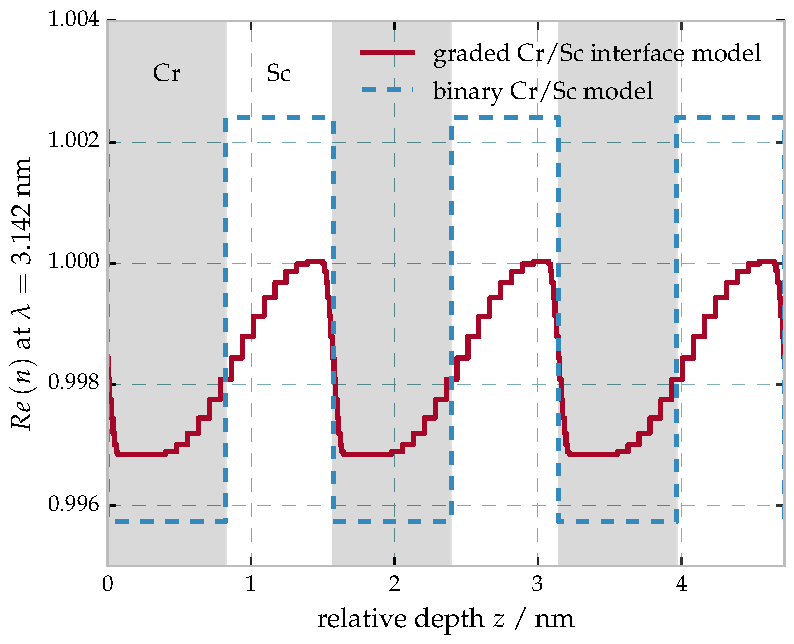
\includegraphics[width=0.7\textwidth]{img/CrSc_binary_vs_fitted_gradual_model}
  \caption{Real part of the index of refraction $n$  based on the results of 
the optimized parameters listed in Table~\ref{tbl:results} for the combined 
analysis for a selected wavelength. The gradual interface model is shown in 
direct comparison to the binary model optimized for the EUV reflectance curve 
over three full periods. The resulting strong asymmetry in the width of the 
interface regions is clearly visible (see text). The gray and white shaded 
areas indicate the Cr and Sc layers, respectively, for the binary model.}
  \label{ch_spec:fig_CrSc_electron_density_profile}
\end{figure}
As mentioned before, the most remarkable result of the combined analysis is the strong asymmetry of the interdiffusion layers. This can only be shown by the combination of all 
analytical experiments conducted here. In addition, the comparison shows that at no point within the periodic multilayer stack pure Sc or pure Cr layers are observed, but always a mixture of both. In the context of answering the question of poor reflectivity with respect to the theoretical possible maximum, this shows that interdiffusion may be the main reason. The loss of contrast with respect to the binary model indicated, causes the diminished reflectivity. We should note, however, that due to the correlation between roughness and interdiffusion this result is still to be verified by the aforementioned analysis of diffuse scattering. This is the topic of chapter~\ref{ch_diff}.

The experiments, methods and findings of this section are part of the publication \fullcite{haase_multiparameter_2016}



%     \chapter{Analysis of Interface Roughness based on Diffuse Scattering} \label{ch_diff}
%With the detailed analysis based on the combination of several complementary experimental methods and the \gls{mcmc} evaluation performed in chapter~\ref{ch_spec}, reconstructions and confidence intervals for the model parameters for all sample systems could be obtained. It was found that roughness and intermixing are of high relevance to explain the diminished reflectivity observed. Most prominently, the interface morphology in the Mo/Si/C sample system from Sec.~\ref{ch_spec:sec_mo_si_c} had a large effect on the reflectivity behavior in both the polished and unpolished case. We attributed the observations to the occurrence of a crystallization process in the molybdenum layer, which affects the interface morphology. Similarly, in case of the Cr/Sc mirror system presented in Sec.~\ref{ch_spec:sec_CrSc}, intermixing or interdiffusion and roughness were attributed to cause the large gap between theoretical reflectivity predictions and actual values measured in the experiments.

So far, no distinction could be made between intermixing and roughness at the surface or interfaces. As discussed in detail in Sec.~\ref{ch_spec:sec_CrSc_results}, this distinction based on the employed structural characterization methods from chapter~\ref{ch_spec}, such as \gls{euv} reflectivity, \gls{reuv}, \gls{xrr} and \gls{xrf}, is in fact not possible due to the lack of sensitivity of the experiments conducted there not even for the combination of all methods. Due to the comparatively large beam footprint on the sample in comparison to interfacial roughness on the nanoscale, any specular reflection measurement, and even the measurement of fluorescence radiation generated by a standing wave field, is only sensitive to the average of the interfacial profile and can thus not be distinguished from horizontally homogeneous intermixing. Effectively, both cases can be described with a gradual profile in the optical constants at the interfaces. Consequently, all methods applied so far rely on a horizontally homogeneous medium model, which was reconstructed. The correlation of the roughness parameter $\sigma$ and the intermixing parameter $\eta$ in Fig.~\ref{ch_spec:fig_CrSc_eta_rho_correlation} nicely demonstrate that assessment.

Within this chapter, we investigate the diffuse scattering contribution measured from all samples studied in chapter~\ref{ch_spec}. While none of the experiments conducted there could yield a distinction criterion, diffuse scattering can only be observed from rough surfaces or interfaces, while intermixing does not cause any off-specular intensity contribution. The analysis of the diffuse scattering, here in particular scattering in the \gls{euv} spectral range, therefore serves as a natural tool to implement the distinction of intermixing on the one hand and roughness on the other. In addition, the distribution of the scattered intensity contains information on the morphology of roughness which is of particular interest to understand the effect on the reflectivity as observed in the previous chapter. First, we continue the analysis of the Mo/B$_4$C/Si/C sample based on the layer model derived in Sec.~\ref{ch_spec:sec_reconstruction_PTB17} and demonstrate in detail the effects observed in case of diffuse \gls{euv} scattering from multilayer systems with an analysis based on the theory introduced in Sec.~\ref{ch_theo:sec_diffuse_scattering}. In the second part, we investigate the two sample sets with systematically varied molybdenum thickness from Sec.~\ref{ch_spec:sec_mo_si_c}. We specifically focus on the role of the interphase morphology in the diminished reflectivity observed for some of the samples in the two sets of Mo/Si/C systems. Furthermore, the effect of the polishing process in one of the sample sets is addressed. Finally, we investigate the parameter correlation of intermixing and roughness for the Cr/Sc sample and finalize the characterization made in Sec.~\ref{ch_spec:sec_CrSc_results} based on the diffuse scattering from that sample.


\section{Near-normal Incidence Diffuse Scattering} \label{ch_diff:sec_PTB17}
In the theoretical description of diffuse scattering in chapter~\ref{ch_theo}, we have elaborated on the characterization of the scatter intensity from a multilayer sample. The goal of the investigation of the diffuse scattering intensity is to gain information on the interface morphology in the sample. In Sec.~\ref{ch_theo:sec_elastic_scattering}, the measured scattering intensity $I_\text{s}$ is described in terms of the differential scattering cross section $\big(\frac{d \sigma}{d \Omega}\big)$, which is given explicitly for the problem of interfacial and surface roughness in multilayer samples in Eq.~\eqref{ch_theo:eqn_full_dwba_expression}. As indicated there, the full theoretical description is based on the introduction of the reciprocal space as an adapted set of coordinates for the scattering problem. This space is spanned by the coordinates $q_x$, $q_y$ and $q_z$. Those are the components of the momentum transfer due to the scattering process (cf.~Sec.~\ref{ch_theo:sec_diffuse_scattering}) and are related to the experimental parameters wavelength $\lambda$, as well as the angle of incidence $\alpha_i$ and the exit angle $\alpha_f$ of the scattering experiment. Based on the theory developed in Sec.~\ref{ch_theo:sec_diffuse_scattering}, a mapping of reciprocal space along the two coordinates $q_x$ and $q_z$ is required to obtain information on the samples interface morphology.

In order to discuss the diffuse scattering experiments and enable a theoretical analysis, we shall therefore first give some definitions of measurement geometry and how it is related to the reciprocal space coordinates. So far, any scattering measurement (excluding the \gls{xrf} experiment) of chapter~\ref{ch_spec} was conducted in the specular reflection geometry, where incidence and exit angle are equal, i.e.~at $q_x = q_y \equiv 0$. Diffusely scattered radiation caused by roughness, however, is scattered to off-specular angles. The experiments conducted here are exclusively done in a co-planar geometry since the roughness in the samples under investigation is assumed to be isotropic in the directions parallel to the surface (cf.~Sec.~\ref{ch_theo:sec_diffuse_scattering}). Thus, any scattered radiation is only measured in the scattering plane defined by the incidence wave vector and the surface normal of the multilayer sample. Two different types of measurements need to be distinguished as they relate to different paths through reciprocal space, the \emph{detector scan} geometry and the \emph{rocking scan} geometry both indicated in Fig.~\ref{ch_diff:fig_scattering_geometry}.
\begin{figure}[htbp]
    \def\svgwidth{0.6\textwidth}
    \import{svg/}{Streugeometrie_diffuse.pdf_tex}
    \caption{Co-planar measurement geometries. By keeping the opening angle $\Delta\Theta = \alpha_i + \alpha_f$ between incident and exit beam and the detector fixed, respectively, a rocking scan can be performed by changing the sample angle $\omega$. In a detector scan the sample angle $\omega$ is kept fixed and defines the angle of incidence while the detector is moved along $\Theta$.}
    \label{ch_diff:fig_scattering_geometry}
\end{figure}
The detector scan describes a movement of the detector inside the scattering plane recording radiation scattered to the exit angle $\alpha_f$, while keeping the incidence angle $\alpha_i$ constant and is indicated by the red shaded area in Fig.~\ref{ch_diff:fig_scattering_geometry}. The rocking scan refers to a rotation of the sample around the axis perpendicular to the scattering plane while keeping the detector position fixed with respect to the incident beam (indicated by the blue shaded are in Fig.~\ref{ch_diff:fig_scattering_geometry}). The angle between detector and the incident beam is referred to as $\Delta \Theta = \alpha_i + \alpha_f$, while the tilt angle of the sample is $\omega$. By changing $\omega$, the incidence angle $\alpha_i$ and the exit angle $\alpha_f$ are changed accordingly. In both cases this leads to incidence and exit angles, which are no longer equal and, thus, non-vanishing values for the $q_x$ vector component. The out-of-plane angle $\theta_f$ (cf.~Fig.~\ref{ch_theo:fig_scattering_process} in Ch.~\ref{ch_theo}) remains zero in those experiments and consequently $q_y \equiv 0$.

The corresponding paths through reciprocal space, calculated according to Eq.~\eqref{ch_theo:eqn_q_components}, are different for these two cases. They are shown schematically in Fig.~\ref{ch_diff:fig_pathsInQ} for two exemplary experimental parameter sets of incidence angle $\alpha_i$ and opening angle $\Delta \Theta$, respectively,  as well as wavelength for the two scan types.
\begin{figure}[htbp]
    \def\svgwidth{0.7\textwidth}
    \import{svg/}{Qspace_paths.pdf_tex}
    \caption{Schematic positions in reciprocal space (cf.~Eq.~\eqref{ch_theo:eqn_q_components}) in dependence on the measurement geometry. The dashed path represents a rocking scan with the angle $\omega$. The solid line shows the movement in $q$-space when changing the detector angle $\alpha_f$ at a fixed angle of incidence. By tuning the wavelength at each angular position, the $q_z$-direction becomes accessible as indicated by the dotted arrows.}
    \label{ch_diff:fig_pathsInQ} 
\end{figure}
Clearly, for a mapping of the two-dimensional space spanned by $q_x$ and $q_z$ it does not suffice to perform only angular scans. In addition, wavelength scans ($\lambda$-scan) have to be performed at each angular position. By changing the wavelength and the angle in the same measurement, both degrees of freedom ($q_x$ and $q_z$) in reciprocal space become accessible.

Based on the theory in Sec.~\ref{ch_theo:sec_diffuse_scattering}, interface roughness contributes to the scattering intensity by introducing momentum transfer parallel to the surface. The \gls{psd}, describing this statistical roughness, is thus in our co-planar geometry only dependent on $q_x$\footnote{The \gls{psd} is generally dependent on $q_\parallel = \sqrt{q_x^2+q_y^2}$, which reduces to $q_\parallel \equiv q_x$ in co-planar geometry}, i.e.~the momentum transfer within the interface planes. In the theory chapter, we have derived an expression for the \gls{psd}, which describes an average value across all interfaces of the multilayer. While individual \gls{psd}s can be described within the theoretical framework, this poses an ill-defined model for the experiments conducted here. In all measurements taken, many interfaces contribute to the diffuse scattering intensity simultaneously. The periodic character of the multilayer systems, does not allow to distinguish the individual contributions as the wave field inside the multilayer exhibits the same periodicity. The experiment thus delivers a contribution across all interfaces, which makes a distinction of individual interfaces impossible. In addition to that assessment, the model of a single average \gls{psd} is found to be justified in case of high degree of vertical correlation throughout the stack, which we shall confirm through the appearance of the corresponding resonant features in our experiments.

Based on the \gls{psd} as derived in Eq.~\eqref{ch_theo:eqn_psd} with the dependence only on $q_x$, we should expect to be able to extract its values from the measured data as cuts along the $q_x$ axis anywhere in a measured reciprocal space map. However, it was observed in grazing incidence diffuse x-ray scattering experiments, that vertical correlation of roughness causes an additional intensity modulation of the scattering in reciprocal space along the $q_z$ direction, the so-called \emph{Bragg sheets} \cite{jiang_nonspecular_1992, holy_nonspecular_1994, salditt_kinetic_1994, holy_interface_1995}.
\begin{figure*}[htb]
    \def\svgwidth{\textwidth}
    \import{svg/}{Bragg_sheets_explained.pdf_tex}
    \caption{Schematic illustration of the appearance of Bragg-sheets in the off specular scattering intensity at the $q_z$ value fulfilling the Bragg condition of the multilayer stack. The width $\delta q_z$ of the sheet is dependent on the degree of vertical correlation of roughness.}
    \label{ch_diff:fig_Bragg_sheets_explained} 
\end{figure*}
As the interfaces have periodic distances along the surface normal of the sample, roughness correlation poses a Bragg condition with respect to the $q_z$ component of the momentum transfer vector enhancing the diffuse scattering where fulfilled. The expected diffuse scattering distribution in reciprocal space is schematically depicted in Fig.~\ref{ch_diff:fig_Bragg_sheets_explained}. Since the periodicity of the interfaces is the multilayer periodicity, those Bragg sheets are expected to appear, where the first and higher order Bragg condition of the multilayer is fulfilled, i.e.~where inside the multilayer $q_z=m 2 \pi /\tilde{D}$. Here, $m$ is the integer number of the Bragg order and $\tilde{D} = \tilde{n}_i d_i + \tilde{n}_j d_j$ is the optical multilayer period thickness in real space, where $\tilde{n}_i$ and $\tilde{n}_j$ are the real part of the index of refraction of the respective layer $i$ and $j$. Those sheets of increased intensity appearing in reciprocal space vary in width along $q_z$ depending on the strength of the correlation of roughness along the vertical direction in the sample. The higher the correlation length $\xi_\perp$, the thinner is the Bragg sheet in $q_z$ direction (cf.~upper and lower part of Fig.~\ref{ch_diff:fig_Bragg_sheets_explained}), i.e.~the smaller is $\delta q_z$. In the theoretical treatment of the diffuse scattering in Sec.~\ref{ch_theo:sec_diffuse_scattering}, this vertical roughness correlation length $\xi_\perp(\vec{q}_\parallel)$ enters through the replication factor $c_{ij}^{\perp}(\vec{q}_\parallel)$ in Eq.~\eqref{ch_theo:eqn_factorized_structure_factor} and was explicitly given in Eq.~\eqref{ch_theo:eqn_replication_factor}. Due to the strong enhanced intensity in those Bragg sheets, the \gls{psd} is preferably extracted as a vertical cut along $q_x$ at the $q_z$ position of the sheet \cite{salditt_kinetic_1994,siffalovic_characterization_2009}. Consequently, in the following we shall focus on the mapping of reciprocal space in the vicinity of the first Bragg resonance to observe the expected Bragg-sheet intensity distribution and analyze the interface morphology.

In the studies cited above, the reciprocal space maps of multilayer diffuse scattering were obtained in a grazing incidence geometry using X-rays. The major disadvantage of this technique is that curved samples are not accessible in that way, since no grazing incidence measurement can be conducted if the sample is convexly curved. Here, the diffuse scattering is studied using \gls{euv} radiation impinging at near-normal incidence. Thereby, this disadvantage is overcome. However, as explained above, using near-normal incidence radiation reduced the accessible $q_z$ range for constant wavelength, which can be compensated by tuning the wavelength accordingly, whereas grazing incidence studies reveal the Bragg sheets in the out-of-plane direction at fixed photon energies, e.g.~\textcite{siffalovic_characterization_2009}.

\subsection{Mapping Reciprocal Space for the Mo/B$_4$C/Si/C Sample}
In this section, the \gls{euv} diffuse scattering from the Mo/B$_4$C/Si/C sample, structurally characterized using \gls{euv} reflectivity in Sec.~\ref{ch_spec:sec_PTB17}, is investigated as an example for the analysis of near-normal scatter intensity from multilayer samples. Diffuse scattering measurements in three different geometries were conducted at the \gls{sx700} beamline at \gls{bessy}. From the experimental data, the respective reciprocal space coordinates were calculated and the corresponding maps and the experimental details are given in Fig.~\ref{ch_diff:fig_PTB17_detector_and_rocking_maps}.
\begin{figure*}[htbp]
        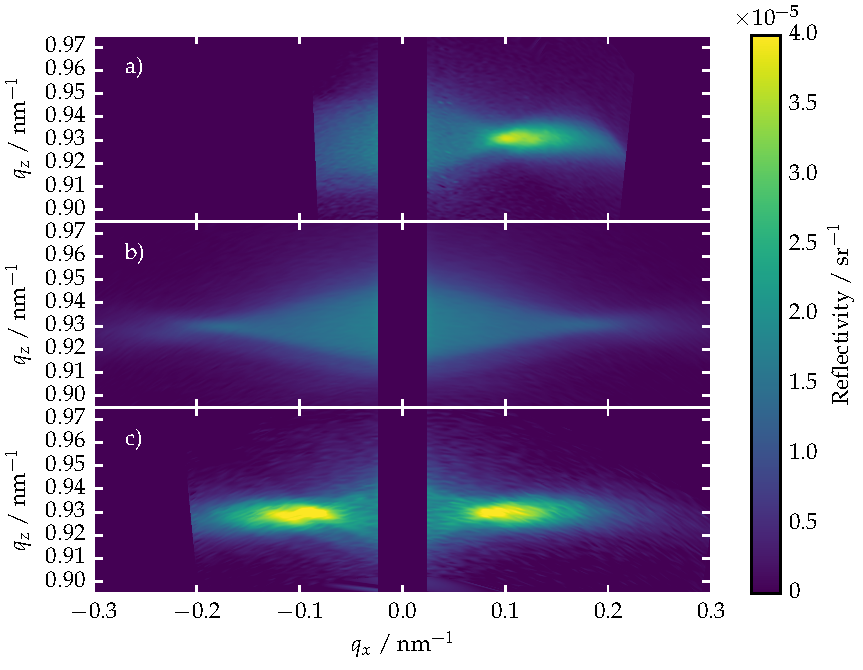
\includegraphics[width=\textwidth]{img/PTB17_diffuse_scattering_multiple_geometries} \caption{Measured intensity map of a detector scan of the Mo/B$_4$C/Si/C multilayer mirror at an angle of incidence $\alpha_i = 6.75^\circ$ (a) and measured intensity maps of the identical sample obtained through rocking scans at an opening angle between detector and incident beam of $\Delta \Theta = 13.5^\circ$ (b) and $\Delta \Theta = 30^\circ$ (c). The area close to the specular axis was excluded from this dataset due to its strong intensity compared to the diffuse scattering shown here. The detector scan (a) was performed at an angle of incidence of $\alpha_i = \SI{6.75}{\degree}$ moving the detector from $\alpha_f = \SI{-3.75}{\degree}$ to $\alpha_f = \SI{46.75}{\degree}$ (corresponding to detector angles from $\Delta \Theta = \SI{3.0}{\degree}$ to $\Delta \Theta = \SI{40.0}{\degree}$) in steps of $\SI{0.5}{\degree}$. The access to the negative $q_x$-axis in (a) was limited due clipping of the incoming beam with the detector. The angular ranges for the rocking scan (b) with opening angle $\Delta \Theta = \SI{13.5}{\degree}$ correspond to angles of incidence from $\alpha_i = \SI{-18.0}{\degree}$ to $\alpha_i = \SI{31.5}{\degree}$ in steps of $\Delta\alpha_i = \SI{0.5}{\degree}$. In terms of the rocking angle $\omega$ this range corresponds to values from $\omega = \SI{-24.75}{\degree}$ to $\omega = \SI{24.75}{\degree}$, where $\omega = \SI{0.0}{\degree}$ corresponds to the specular reflection geometry ($\alpha_i = \alpha_f$). For the second rocking scan geometry (c) with $\Delta \Theta = \SI{30.0}{\degree}$, the angle of incidence was varied from $\alpha_i = \SI{-3.0}{\degree}$ to $\alpha_i = \SI{27.5}{\degree}$ (corresponding to $\omega = \SI{-18.0}{\degree}$ to $\omega = \SI{12.5}{\degree}$) in steps of $\SI{0.5}{\degree}$. At each angular position of the aforementioned angular scan geometries, a wavelength scan between \nm{12.4} and \nm{14.0} was conducted using a step size of $\Delta \lambda = \nm{0.01}$.  A GaAsP photo diode with an active area of $\mm{4.5} \times \mm{4.5}$ at a distance to the sample of $\mm{250}$ was used as a detector for the diffusely scattered radiation.} \label{ch_diff:fig_PTB17_detector_and_rocking_maps}
\end{figure*}
The reciprocal space maps for the rocking scan (b) at an opening angle of $\Delta \Theta = 13.5^\circ$ and the rocking scan (c) at an opening angle of $\Delta \Theta = 30^\circ$ and for the detector scan (a) with the angle of incidence $\alpha_i = 6.75^\circ$ clearly show different symmetries rather than the expected Bragg sheet from Fig.~\ref{ch_diff:fig_Bragg_sheets_explained}. Thus, the measurements conducted here stand in contrast to the expectation derived from grazing incidence experiments and outlined in Fig.~\ref{ch_diff:fig_Bragg_sheets_explained}. Instead, a strong enhancement in the off-specular scattering is observed around $q_x\approx \pm 0.1$ nm$^{-1}$ (cf.~(a) and (c)), which is not replicated on the negative $q_x$-axis in case of (a). The rocking scans (b) and (c) are symmetric with respect to the specular axis at $q_x=0$, however, no enhanced scattering appears in (b). The latter map shows a triangular-shaped intensity distribution for both the positive and negative $q_x$ range. A minimum in the width, i.e.~in the quatity $\delta q_z$ defined in Fig.~\ref{ch_diff:fig_Bragg_sheets_explained}, with respect to the $q_z$ direction can be observed in (b) around $q_x \approx \pm 0.2$ nm$^{-1}$. The triangular shape also appears for the positive $q_x$ range of the detector scan in (a), where the minimum in width coincides with the intensity maximum. These observations are in clear contrast to the expectation of an appearance of identical Bragg sheets, independent of the measurement geometry. Clearly, the measurement of diffuse scattering at \gls{euv} wavelengths and near-normal incidence differs from the observations made for grazing incidence experiments using X-rays (cf.~\textcite{salditt_kinetic_1994} or \textcite{jiang_nonspecular_1992}).

Clearly, the measurement geometry used influences the measured reciprocal space maps, even though all maps were recorded for the sample sample with the same spot position. This indicates that the intensity distributions seen here, cannot be the result of multilayer roughness properties alone, i.e.~the \gls{psd}, which do not change due to changes in the illumination geometry. Furthermore, the results from Fig.~\ref{ch_diff:fig_PTB17_detector_and_rocking_maps} are clearly deviating from the expectation sketched in Fig.~\ref{ch_diff:fig_Bragg_sheets_explained}. This indicates, that an additional effect causing a modulation of the diffuse scattering intensity is observed, since intensities caused by roughness occur at identical positions in reciprocal space for any measurement geometry. In fact, the additional modulations of the scatter intensity are caused by the direction from which the radiation impinges on the multilayer structure itself, rather than the roughness properties. We shall therefore investigate this observation here to give an indication for the results found here.

\subsection{Kiessig-like Peaks and Resonant Effects}
To explain the observed off-specular intensity distribution for the multilayer sample investigated here, additional effects exceeding the description of Bragg sheets need to be taken into account. So far, the description of diffuse scattering and enhancement due to correlated roughness was under the assumption of kinematic scattering, i.e.~a single diffuse scattering event. However, multiple reflections at the interfaces may not be ignored. To clarify that, we shall consider two additional processes, which may happen before and after a diffuse scattering event at the interface. Fig.~\ref{ch_diff:fig_kiessig_like_peaks_scheme} illustrates two situations, where the impinging or exiting (diffusely scattered) radiation is in resonance with the multilayers Bragg condition, i.e.~strongly enhanced in intensity.
\begin{figure*}[htb]
    %\def\svgwidth{\textwidth}
    \import{svg/}{Bragg_sheet_sheme.pdf_tex}
    \caption[Illustration of dynamic scattering processes]{Illustration of dynamic scattering processes. In (a), the impinging radiation is resonantly reflected from the multilayer structure by fulfilling the Bragg condition. In (b), certain parts of the diffusely scattered radiation from the interface roughness again fulfills the Bragg condition and is enhanced in intensity.}
    \label{ch_diff:fig_kiessig_like_peaks_scheme}
\end{figure*}
In the first case (a), the impinging radiation fulfills the Bragg condition with respect to angle of incidence and is consequently resonantly reflected from the multilayer mirror. Through this, any diffusely scattered radiation measured at any exit angle would be significantly stronger compared to the situation, where the incidence angle or wavelength does not fulfill the Bragg condition, despite the fact that the roughness itself did not change. In the second case (b), depending on the wavelength some of the diffusely scattered radiation fulfills the Bragg condition of the multilayer and is again reflected resonantly from it causing a major intensity increase. These two processes are a special case of the two situations considered within the \gls{dwba} theory illustrated in Fig.~\ref{ch_theo:fig_dwba_scheme}, termed $R T^*$ and $T R^*$. It should be noted, however, that the processes described there take into account any reflection and transmission at the respective interface. Here, the focus is on the case, where either reflection fulfills the Bragg condition and, thus, is resonantly enhanced.

The effects seen here are the result of multiple (dynamic) reflections inside the multilayer system. They were observed as resonantly enhanced streaks, so-called \emph{Bragg-like lines}, and intense \emph{Bragg-like peaks}. The latter case occurs, where both the conditions illustrated in Fig.~\ref{ch_diff:fig_kiessig_like_peaks_scheme} are fulfilled simultaneously, i.e.~where the Bragg-like lines cross each other. These two phenomena were often observed in diffuse scattering maps from multilayer samples recorded in grazing incidence geometry with X-rays  \cite{holy_nonspecular_1994}. The theoretical principle leading to these off-specular enhancements is also known as the process of \emph{Umweganregung} \cite{baumbach_influence_1994, baumbach_grazing-incidence_1995}. As the fulfillment of the Bragg condition for each Bragg-like line is only dependent on two of the three experimental parameters, i.e.~either the incidence angle $\alpha_i$ or the exit angle $\alpha_f$, in both cases together with the wavelength, the position of those enhancements is different in the reciprocal space map depending on the measurement geometry. In literature \cite{holy_nonspecular_1994, mikulik_x-ray_1997, baumbach_influence_1994, baumbach_grazing-incidence_1995}, such enhancements were so far only observed from the main Bragg resonance of the multilayer, i.e.~the fulfillment of the Bragg condition of the periodic stack. In our case, no higher-order Bragg resonances can be observed, as they would appear as Bragg-like peaks in the off-specular scattering far away from the accessible $q_\parallel$ range of our experiment. However, the two Bragg-like lines corresponding to the first order Bragg peak cross at the position of the specular reflex and otherwise amount to broad bands in the diffuse map as elaborated in the following paragraphs.

\begin{figure}[htbp]
        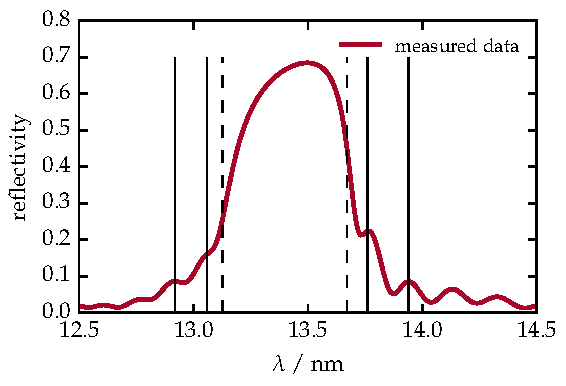
\includegraphics{img/kiessig_like_peaks_reflectivity_curve} \caption{Measured reflectivity curve of the Mo/B$_4$C/Si/C multilayer mirror at an angle of incidence $\alpha_i = 6.75^\circ$. The solid black lines mark the positions of the first two Kiessig-fringes at each side of the main maximum. The dashed lines indicate the \gls{fwhm} position of the main Bragg peak.}
        \label{ch_diff:fig_ptb17_reflectance_AOI_675} 
\end{figure}
Apart from the main Bragg peak, additional resonances are observed in the \gls{euv} reflectivity curve as shown in Fig.~\ref{ch_diff:fig_ptb17_reflectance_AOI_675} (marked with solid vertical lines). Those side peaks, known as Kiessig fringes \cite{kiessig_interferenz_1931}, correspond to the interference of radiation reflected from the top surface and the substrate interface, as previously discussed in Sec.~\ref{ch_spec:sec_PTB17}. The dynamic enhancement, equivalent to the Bragg-like lines and Bragg-like peaks for the main maximum, expected for those side fringes is very well within the measured reciprocal space ranges of our measurements geometries and wavelengths. In analogy to the names given to those effects originating from the main Bragg resonance, they shall be called \emph{Kiessig-like lines} and \emph{Kiessig-like peaks} here. In Fig.~\ref{ch_diff:fig_kiessig_like_peaks_diffuse_map}, the positions where those enhancements are to be expected in the maps, shown originally in \ref{ch_diff:fig_PTB17_detector_and_rocking_maps}, are indicated as white solid lines for the first two fringes on either side of the reflectivity curve maximum. In addition, the \gls{fwhm} of the main Bragg maximum was marked with dashed lines, both in Fig.~\ref{ch_diff:fig_ptb17_reflectance_AOI_675} and in Fig.~\ref{ch_diff:fig_kiessig_like_peaks_diffuse_map} to mark the limits of the two aformentioned Bragg-like lines observable in this scattering map.
\begin{figure*}[htbp]
        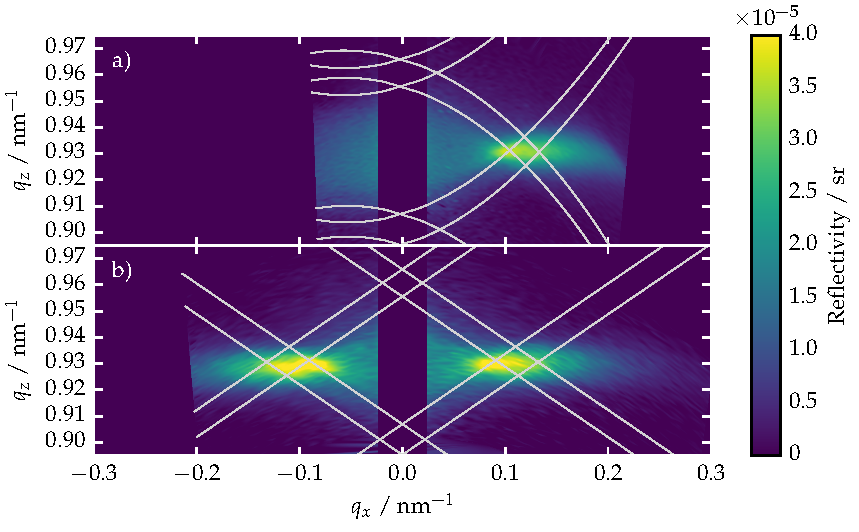
\includegraphics[width=\textwidth]{img/kiessig_like_peaks_diffuse_map} \caption{Measured intensity maps of Fig.~\ref{ch_diff:fig_PTB17_detector_and_rocking_maps} with the calculated positions of the Kiessig-like lines (solid lines) for the Kiessig fringes marked in Fig.~\ref{ch_diff:fig_ptb17_reflectance_AOI_675} and the Bragg-like lines (bands between the dashed lines). The positions, where the solid lines cross show the Kiessig-like peaks positions. The area contained within the dashed lines in the center of each plot correspond to the Bragg-like peak of the first Bragg order of the multilayer and explain the triangular or diamond shaped area of increased intensity (see main text).} \label{ch_diff:fig_kiessig_like_peaks_diffuse_map} 
\end{figure*}

Clearly, the off-specular enhancement observed in Fig.~\ref{ch_diff:fig_kiessig_like_peaks_diffuse_map}a and \ref{ch_diff:fig_kiessig_like_peaks_diffuse_map}c fits to some of the theoretically predicted appearances of the Kiessig-like peaks, i.e.~at the crossing points of the Kiessig-like lines (white solid lines). However, at other crossing points or in Fig.~\ref{ch_diff:fig_kiessig_like_peaks_diffuse_map}b no strong visible enhancement appears. The reason for that is, that the diffuse scattering map is the result of several overlapping effects. A strong enhancement is only observed where, in addition to the Kiessig-like peaks,   also a Bragg sheet, due to correlated roughness in the sample, appears. The intensity distribution along $q_x$ for the Bragg sheet, as outlined above, is governed by the \gls{psd} and decays with increasing absolute values of $q_x$ in positive and negative direction. Consequently, while an enhancement due to Kiessig-like peaks also exists in Fig.~\ref{ch_diff:fig_kiessig_like_peaks_diffuse_map}b, their positions are at larger positive and negative $q_x$ values, where the intensity of the Bragg sheet has already decayed. A similar case can be made for Kiessig-like peaks far away from the vertical, i.e.~$q_z$, position of the Bragg sheet. As discussed above, highly correlated roughness limits the width $\delta q_z$ of the sheet. Thus, Kiessig-like peaks above or below the $q_z$ position of the sheet, where the its intensity has dropped, may cause enhancement, but it is below the detection threshold.

The aforementioned broad bands corresponding to the Bragg-like lines of the main Bragg resonance appear in between the dashed lines. Indeed, most prominently visible in Fig.~\ref{ch_diff:fig_kiessig_like_peaks_diffuse_map}b, the triangular shaped intensity distribution in the center of the map is in fact the result of resonant enhancement due to the first order Bragg-like peak, which extents across a large area of the map in this case.
The diffuse scattering distribution in the reciprocal space maps is thus a combination of dynamic effects (the first-order Bragg-like peak and the Kiessig-like peaks) and kinematic effects~(Bragg sheets).

As indicated above, the processes described here are contained in the theoretical description given in Eq.~\eqref{ch_theo:eqn_full_explicit_dwba_with_approximations} in Sec.~\ref{ch_theo:sec_diffuse_scattering}. They correspond to the contributions of the \gls{dwba} differential cross section through the processes shown in Fig.~\ref{ch_theo:fig_dwba_scheme}, labeled $R T^*$ and $T R^*$ (Kiessig-like lines, Bragg-like lines) and $R R^*$ (Kiessig-like peaks, Bragg-like peaks). The Bragg-sheets, however, are described as a simple fulfillment of the Bragg condition due to the momentum transfer at the interfaces according to the semi-kinematic description labeled $T T^*$. In order to assess the contribution of dynamic multiple reflections within the stack, we compared the semi-kinematic approximation in Eq.~\eqref{ch_theo:eqn_semi_kinematic_dwba_expression} with the dynamic calculations in Eq.~\eqref{ch_theo:eqn_full_explicit_dwba_with_approximations}. In the semi-kinematic case, all multiple reflection effects are ignored in the differential cross section. The result is the intensity distribution as expected from the kinematic case, however including the accurate transmitted field amplitudes at each interface instead of only a plane wave field amplitude as in the simple Born approximation. 

To evaluate and illustrate the contribution of multiple (dynamic) reflections due to the subsidiary maxima in comparison to the semi-kinematic case, which ignores those effects, Fig.~\ref{ch_diff:fig_kiessig_like_peak_along_qx}b shows a calculated intensity distribution along $q_x$ at $q_z=0.93$ nm$^{-1}$ for the sample investigated here, employing the theoretical framework of the \gls{dwba}, as introducted in Sec.~\ref{ch_theo:sec_diffuse_scattering}.
\begin{figure*}[htbp]
        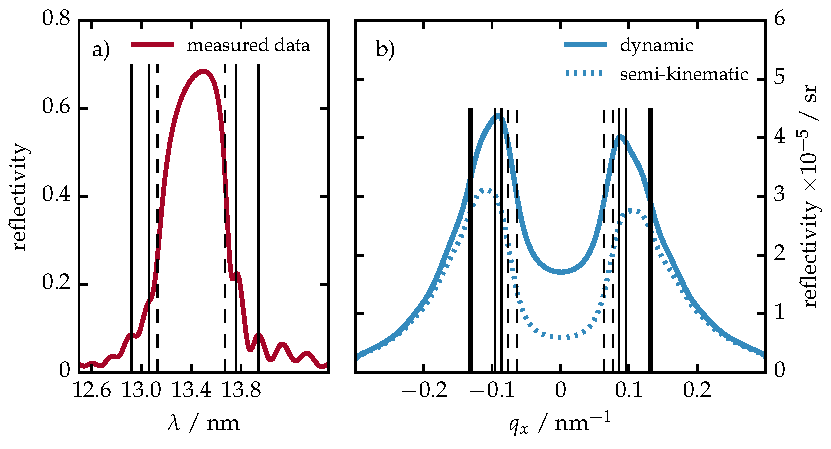
\includegraphics[width=\textwidth]{img/qx_kinematic_vs_dynamic}
        \caption{a) \gls{euv} reflectivity curve with the positions of the \gls{fwhm} of the Bragg peak (dashed black lines) and the positions of the first two Kiessig fringes on each side of the main maximum (solid black lines) similar to Fig.~\ref{ch_diff:fig_ptb17_reflectance_AOI_675}. b) Calculated scattering intensity distribution at $q_z=0.93$ nm$^{-1}$. The solid blue line shows the result of the dynamic calculation for a rocking scan with an opening angle of $\Delta\Theta=30^\circ$. The dashed blue line represents the calculation applying the semi-kinematic approximation, ignoring any multiple reflections within the multilayer. The dashed vertical lines are the position of the main Bragg peaks \gls{fwhm}, while the solid vertical lines show the position of dynamic contributions of the Kiessig fringes close to the main maximum. Each Kiessig fringe marked in the inset appears for the corresponding positive and negative $q_x$ value. The strong intensity at $|q_x|\approx0.1$ nm$^{-1}$ results from the overlap of the dynamic maxima of two different Kiessig fringes (see text).} \label{ch_diff:fig_kiessig_like_peak_along_qx} 
\end{figure*}
This calculation corresponds to a horizontal cut at $q_z=0.93$ of the measured reciprocal space map shown in Fig.~\ref{ch_diff:fig_kiessig_like_peaks_diffuse_map}c, i.e.~the rocking scan geometry with an opening angle of $\Delta \Theta = \SI{30}{\degree}$. The structural parameters used in this calculation were determined in Sec.~\ref{ch_spec:sec_PTB17} for this sample. At this point, no explaination was given yet on how the parameters of the \gls{psd}, required to perform this calculation, were obtained. Instead, to first emphasize the origin and impact of the dynamic effects, this will be posponed here and discussed in datail in the following Sec.~\ref{ch_diff:sec_determination_of_the_psd} of this chapter. The \gls{euv} reflectivity curve with the marked positions of the Kiessig fringes and the \gls{fwhm} of the man Bragg peak are repeated in Fig.~\ref{ch_diff:fig_kiessig_like_peak_along_qx}a for reference.
The solid blue line corresponds to the dynamic theory, while the dotted blue line is the result of the semi-kinematic calculation. The dashed vertical lines indicate the limits of the main Bragg peaks \gls{fwhm}. The vertical black lines show the position of the Kiessig-like lines intersecting the cut position. Each of the marked fringes in Fig.~\ref{ch_diff:fig_kiessig_like_peak_along_qx}a appears on the negative and positive $q_x$-axis in Fig.~\ref{ch_diff:fig_kiessig_like_peak_along_qx}b. This is caused by the incidence and exit angle, respectively, being at the resonance angle of the various Kiessig maxima in the reflectivity curve as illustrated in Fig.~\ref{ch_diff:fig_kiessig_like_peaks_scheme}. A strong increase with respect to the semi-kinematic approximation is observed. The position of the dynamic contribution from the first 
Kiessig fringes on either side of the main resonance exhibits a pronounced maximum in the diffuse scattering. These fringes contribute most due to their high overall relative 
intensity compared with the fringes further away from the reflectivity maximum. In addition, the position in reciprocal space coincides with the first two Kiessig fringes marked on either side of the main maximum. The contribution by the main Bragg resonance, i.e.~the Bragg-like peak amounts to approximately $\SI{100}{\percent}$ intensity increase at $q_x=0$. The comparison to the semi-kinematic case reveals another reason for the strong intensity of the Kiessig-like peaks compared to the Bragg-like peak. In between the dashed lines on the positive and negative $q_x$ axis in Fig.~\ref{ch_diff:fig_kiessig_like_peak_along_qx}b, a significant decrease of kinematically scattered radiation is observed. The reason for that is a strongly diminished penetration depth of the radiation into the multilayer at the Bragg resonance, which causes less rough interfaces to contribute to the diffuse scattering. This directly counteracts the resonant enhancement due to the Bragg-like peak and leads to an overall lower scattering contribution at these positions in reciprocal space.

Similarly to the calculated intensity distribution for a horizontal cut, a vertical cut at fixed $q_x$ position further emphasizes the importance of taking dynamic effects into account. Fig.~\ref{ch_diff:fig_comparison_full_semi} shows that line cut, perpendicular to the one shown in Fig.~\ref{ch_diff:fig_kiessig_like_peak_along_qx}, along the $q_z$ at $q_x=0.05$ nm$^{-1}$ assuming a measurement geometry corresponding to the rocking scan with opening angle $\Delta \Theta = \SI{30}{\degree}$ (cf.~Fig.~\ref{ch_diff:fig_kiessig_like_peaks_diffuse_map}c). Again, the structural data was taken from the analysis in Sec.~\ref{ch_spec:sec_PTB17}.
\begin{figure}[htbp]
        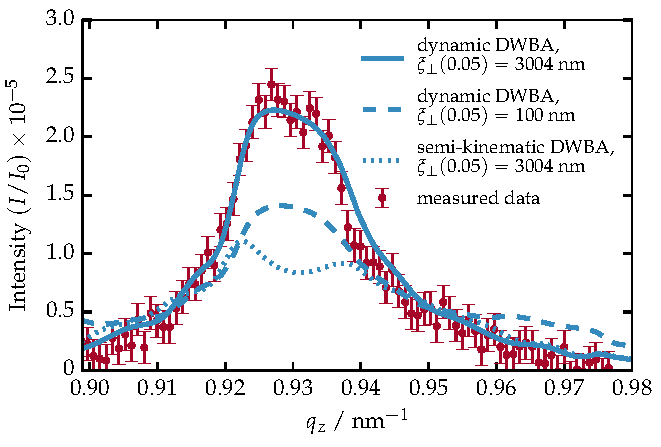
\includegraphics{img/PTB17_diffuse_qz_kinematic_vs_dynamic_100nm} \caption{Calculated scattering intensity along a vertical cut in $q_z$ with fixed $q_x=0.05$ nm$^{-1}$ for the dynamic and semi-kinematic calculations for a rocking scan of the Mo/B$_4$C/Si/C sample at $\Delta\Theta=30^\circ$.} \label{ch_diff:fig_comparison_full_semi} 
\end{figure}
The results of the calculation including the dynamic effects show distinct differences with an increase up to $\SI{100}{\percent}$ of the calculated scattered intensity close to the multilayer resonance at $q_z=0.93$ nm$^{-1}$ compared to the semi-kinematic calculation. Hence the dominance of the dynamic contributions in the vicinity of the Bragg resonance is also observed here. In addition to comparing the dynamic and semi-kinematic calculations, a dynamic calculation assuming a reduced vertical correlation of roughness was added as dashed blue curve. As discussed in the beginning of Sec.~\ref{ch_diff:sec_PTB17}, the Bragg sheet width is strongly dependent on the amount of correlated interfaces. Clearly, a broadening and reduction of scatter intensity is seen for this case here (dashed line in Fig.~\ref{ch_diff:fig_comparison_full_semi}). This shows, that the Bragg sheet is in fact still visible but obscured by the dominant structure in the diffuse scattering caused by the dynamic effects explained above.

\subsection{Reconstruction of the PSD and the Multilayer Enhancement Factor}
\label{ch_diff:sec_determination_of_the_psd}
Within the framework of the \gls{dwba}, considering the dynamic effects, the full expression for the differential cross section of the diffuse scatter is given in Eq.~\eqref{ch_theo:eqn_full_explicit_dwba_with_approximations}. As discussed above, the power spectral density only becomes accessible through the diffuse scattering measurements, if the structural properties of the multilayer are known. Those were determined for all samples in this thesis with the methods described in chapter~\ref{ch_spec}. Based on those results, the differential cross section allows to calculate the scattering intensity maps, which were measured here and therefore enable the reconstruction of the \gls{psd}.

The large impact of resonant effects on the off-specular scattering intensity measured in the three geometries shown above prove, that multiple reflections have to be taken into account to extract the contribution of the interface morphology and determine a \gls{psd}. To better understand the effects involved here, we shall analyze the intensity curves for all three measurement geometries based on a horizontal cut along $q_x$ at the position of $q_z=\SI{0.93}{\nano\meter^{-1}}$, which corresponds to the momentum transfer at the multilayer resonance. As illustrated in the schematic explanation in Fig.~\ref{ch_diff:fig_Bragg_sheets_explained}, this coincides with the horizontal position of the the Bragg sheet and its maximum intensity. In the case shown there, the \gls{psd} could just be extracted from a horizontal cut of the scatter intensity at that position. This has been done by \textcite{siffalovic_characterization_2009}, for example, in the case of \gls{gisaxs} measurements. Similarly to this approach, the calculated intensity curves corresponding to such a horizontal cut in the three geometries measured here including the dynamic effects, are shown in direct comparison in Fig.~\ref{ch_diff:fig_PTB17_qx_cuts_different_geometries}.
\begin{figure}[htbp]
	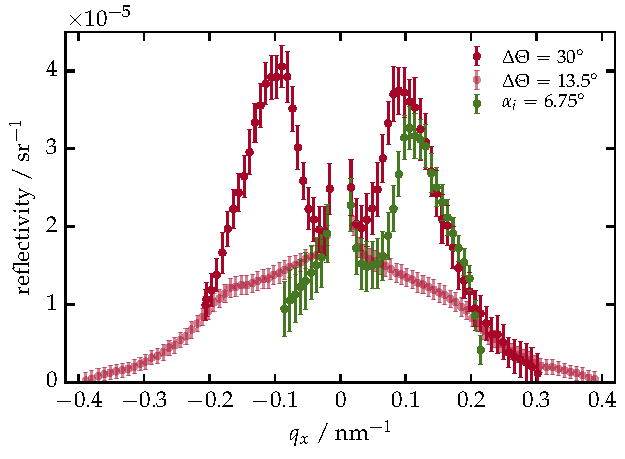
\includegraphics{img/PTB17_diffuse_BraggSheet_DetectorAndRocking} \caption{Averaged diffuse scattering intensity along $q_x$ in the interval  $q_z=(0.930 \pm 0.003$) nm$^{-1}$ corresponding to the resonance of the multilayer. The data shown are two rocking scan and one detector scan geometries (see text for details).} \label{ch_diff:fig_PTB17_qx_cuts_different_geometries}
\end{figure}
The strong off-specular enhancement of scattering intensity obstructing the underlying \gls{psd} is clearly visible here for the detector scan geometry and the rocking scan with opening angle of $\Delta\Theta = \SI{30.0}{\degree}$. In case of the second rocking scan with $\Delta\Theta = \SI{13.5}{\degree}$, only a small shoulder can be observed at $q_x \approx \pm \SI{0.2}{\nano\meter^{-1}}$.

In the theoretical treatment of the diffuse scattering in Sec.~\ref{ch_theo:sec_diffuse_scattering}, we have derived an expression for the differential cross section based on the \gls{dwba} in Eq.~\eqref{ch_theo:eqn_full_explicit_dwba_with_approximations}. It separates the dynamic enhancements and penetration depth considerations from the power spectral density contribution. It can be divided in two parts of interest. The factor contained in rectangular brackets is the dynamic and kinematic part due to the scattering properties from a multilayer and only dependent on the multilayer layout and vertical roughness correlation, we shall therefore refer to it as \emph{multilayer enhancement factor}. The remaining term, $C(q_x)$, is the average power spectral density and describes the average interface morphology.

To illustrate the impact due to the presence of the multilayer and the geometry dependence, the result of calculations of the multilayer enhancement factor alone, based on the layer model of our multilayer sample, is shown in Fig.~\ref{ch_diff:fig_PTB17_multilayer_enhancement_factor} for the detector scan and the two rocking scan configurations. The multilayer enhancement factor was normalized with respect to $q_x=0$, i.e. the calculated diffuse scattering contribution on the specular axis.
\begin{figure}[htbp]
	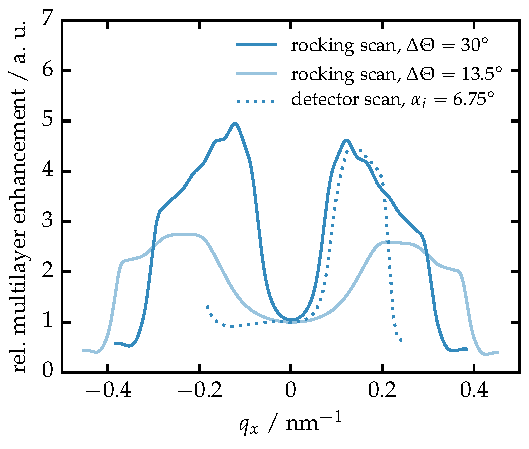
\includegraphics{img/PTB17_multilayer_enhancement_factor} \caption{Enhancement factor due to the specific properties of multilayer reflectivity for three different measurement geometries. The simulations shown here were normalized with respect to the diffuse contribution to the specular reflectivity at $q_x=0$.} \label{ch_diff:fig_PTB17_multilayer_enhancement_factor} 
\end{figure}
It should be noted here, that the abrupt decrease observed for each of the curves towards higher $q_x$ values is not the result of a breakdown of vertical correlation. Instead, it marks the point in reciprocal space for each geometry, respectively, where the photon energy is in resonance with the Si-L edge causing a strong increase of absorption and thus a sharp decrease of the penetration depth into the multilayer. As a result, diffuse scattering intensity is decreased significantly.

The results of the calculation above show that the diffuse scattering from these multilayer mirror systems at near-normal incidence exhibits strong enhancement due to the intrinsically limited bandpass of reflectivity and high reflectance. If both the incidence and exit angle is out of the Bragg resonance, the higher penetration depth of the multilayer causes an increase in the number of interfaces contributing to the diffuse scattering intensity. Thus higher total scattering is observed. The Kiessig fringes and the main Bragg peak cause modulations in the enhancement factor resonantly increased by the purely dynamic processes described in the previous section. Based on these calculations, the cuts along $q_x$ in the measured maps shown in Fig.~\ref{ch_diff:fig_PTB17_qx_cuts_different_geometries} could be normalized by diving the measurement through the calculated multilayer enhancement factor to extract the \gls{psd} of the sample. The result is shown in Fig.~\ref{ch_diff:PTB17_PSD_for_all_geometries} for the positive $q_x$ range.
\begin{figure}[htbp]
	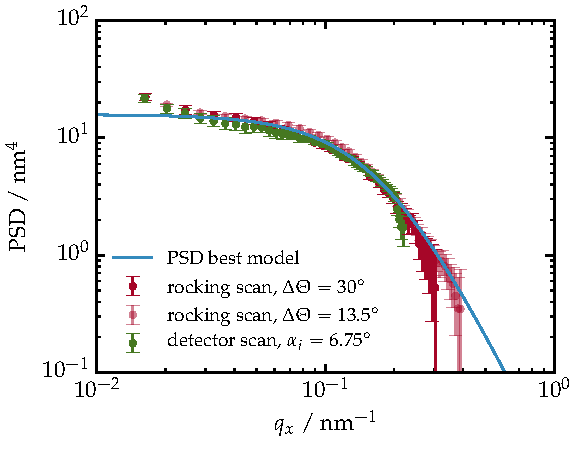
\includegraphics{img/PTB17_PSD_for_all_geometries} \caption{Diffuse scattering intensity corrected for the multilayer enhancement factor. The blue solid line corresponds to a power spectral density with $\xi_\parallel=5.6$ nm, $H=1.0$, $\sigma=0.2$ nm and a vertical correlation length of $\xi_\perp(q_x)=7.5/q_x^2$ nm$^{-1}$.} \label{ch_diff:PTB17_PSD_for_all_geometries} 
\end{figure}
Clearly, this result shows a consistent determination for the \gls{psd} independent of the measurement geometry applied. The individual cuts are in agreement within the measurement uncertainty. Based on the calculation of the multilayer enhancement factor, experimental curves for the \gls{psd} can be extracted as shown in Fig.~\ref{ch_diff:PTB17_PSD_for_all_geometries} without applying a specific model for the interface morphology. However, the measurements conducted here only deliver data in a limited range in the reciprocal space, depending on the selected geometry and wavelengths. To characterize the interface morphology, it is therefore necessary to model the measured data and deduct parameters that relate to the roughness properties. To obtain the \gls{psd} best model reconstruction, the \gls{pso} method was employed similarly to the reconstructions shown in chapter~\ref{ch_spec}.

\subsubsection{Reconstruction of the Power Spectral Density}
It is the goal of this analysis to deduct key properties of the interface roughness, such as vertical and lateral correlation lengths and the \gls{rms} roughness value $\sigma_r$. The latter is directly related to the N\'{e}vot-Croce parameter $\sigma$, which was introduced in Sec.~\ref{ch_theo:sec_multilayer} and determined in the structural reconstruction of chapter~\ref{ch_spec}. There, the roughness is described using this factor. However, intermixing at the interfaces is additionally contained as it can not be distinguished from the roughness. On average of the beam footprint of the specular and fluorescence methods described there, both effects lead to the same decrease in sharpness of the interfaces. Based on the analysis of the \gls{psd} through the diffuse scattering analysis, this distinction can be made. To reconstruct the \gls{psd}, a suitable model has to be introduced for the interface morphology. Here, we apply a fractal interface model, which was found to adequately describe the roughness in case of sputter deposited multilayer systems \cite{de_boer_x-ray_1995, de_boer_x-ray_1996, sinha_x-ray_1988}. It should be noted, that the \gls{psd} for a two dimensional surface should be two-dimensional itself and consider possibly different roughness properties in $x$ ($q_x$) and $y$ ($q_y$) direction. The samples investigated here, however, are fabricated using magnetron sputtering and on rotating sample holders as shown in Sec.~\ref{ch_exp:sec_magnetron_sputtering}. This is important to achieve a homogeneous deposition. We therefore conclude, that roughness on the surfaces and interfaces does not have any predominant direction and may be assumed to be isotropic, i.e.~only dependent on the absolute value of the lateral momentum transfer vector $q_\parallel = \sqrt{q_x^2+q_y^2}$. The \gls{psd} can then be expressed in the closed analytical one-dimensional form as and was introduced in Sec.~\ref{ch_theo:sec_diffuse_scattering} and explicitly given in Eq.~\eqref{ch_theo:eqn_psd}. The three parameters describing the fractal nature of the roughness are the lateral correlation length $\xi_\parallel$, the \gls{rms} roughness $\sigma_r$ and the Hurst factor $H$. The vertical correlation of the roughness parameter $\xi_\perp$ and the off-axis roughness correlation angle $\beta$, defined through Eq.~\eqref{ch_theo:eqn_replication_factor}, Eq.~\eqref{ch_theo:eqn_vertical_roughness_correlation_length_explicit} and Eq.~\eqref{ch_theo:eqn_off_axis_vertical_roughness_correlation_angle}, however, are not included in the \gls{psd} as they are part of the multilayer enhancement factor. Illustrations and explanations of the meaning and effect of these parameters can be found in Sec.~\ref{ch_theo:sec_diffuse_scattering}. In order to fully characterize the system, we therefore analyze the full data set comprising all data points measured for the reciprocal space maps. As explained above, the maps were measured by performing wavelength scans at each angular position of the rocking or detector scans. The result are intensity curves $I_{(\alpha_i, \alpha_f)}(\lambda)$, for each set of angular positions in dependence on the wavelength. The minimization functional $\tilde{\chi}^2$ for each of the three experiments (three diffuse scattering maps), is thus given by
\begin{align}
 \tilde{\chi}^2 = \frac{1}{M-P} \sum\limits_{(\alpha_i, \alpha_f)} \sum\limits_{m} \frac{\big(I_m^\text{model}(\alpha_i, \alpha_f, \lambda)
- I_m^\text{meas}(\alpha_i, \alpha_f, \lambda)\big)^2}{\tilde{\sigma}_m^2} \text{,} \label{ch_diff:eqn_chi_diffuse}
\end{align}
where $M$ is the total number of measurement points, $P$ is the number of optimization parameters and $(\alpha_i, \alpha_f)$ indicates a specific position in the angular detector or rocking scans. The reconstruction was achieved by applying the structural reconstruction from Sec.~\ref{ch_spec:sec_PTB17} and the \gls{pso} technique on the combined set of measurements from all three experiments, i.e.~minimizing the functional $\chi^2 = \tilde{\chi}^2_\text{a} + \tilde{\chi}^2_\text{b} + \tilde{\chi}^2_\text{c}$. The letter indices a, b and c refer to the reciprocal space maps shown in Fig.~\ref{ch_diff:fig_PTB17_detector_and_rocking_maps}. The optimization model parameters are listed in table~\ref{ch_diff:tbl_PTB17_diffuse_optimization_limits_and_results} together with the converged results found.
\begin{table*}
\centering
\caption{Parameters of the DWBA analysis. The lower bound (LB) and upper bound (UB) specify the \gls{pso} parameter space limits.}
\label{ch_diff:tbl_PTB17_diffuse_optimization_limits_and_results}
\begin{tabularx}{\textwidth}{@{}lXrrr@{}}
\toprule
Parameter & Definition & LB & UB & PSO result\\ \midrule
$\sigma_r$ / nm & root mean square roughness & $0.0$& $1.0$ & $0.201$\\ 
$\xi_\parallel$ / nm & lateral correlation length & $0.0$& $20.0$ & $5.579$\\ 
$\xi_\perp$ / nm$^{-1}$ &vertical correlation parameter yielding vertical correlation length trough $\tilde{\xi}_\perp(q_\parallel) = \xi_\perp/q_\parallel^2$ &$0.0$ & $20.0$ & $7.512$\\
$H$ & Hurst factor & $0.0$ & $1.0$ & $1.000$ \\
$\beta$ / $^\circ$&angle for off-axis vertical roughness correlation& $-10.0$ & $10.0$ & $-0.152$\\ 
 \bottomrule
\end{tabularx}
\end{table*}
In Fig.~\ref{ch_diff:fig_PTB17_diffuse_comparisonWithTheory}, the measured reciprocal space maps in the detector scan geometry and the rocking scan geometry are shown in direct comparison with the theoretically calculated maps based on the best model results. 
\begin{figure*}[htbp]
        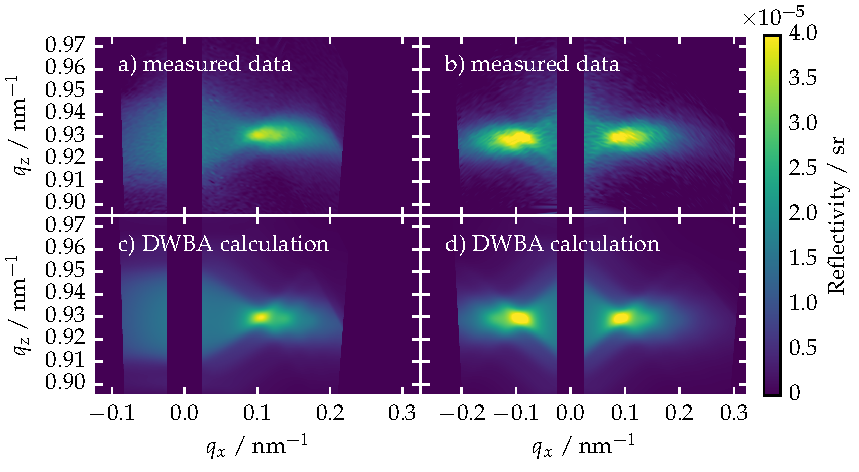
\includegraphics[width=
        \textwidth]{img/PTB17_diffuse_simulation_vs_measurement} \caption{Measured  reciprocal space maps for the detector scan geometry (a) and the rocking scan at an opening angle of $\Delta\Theta=30^\circ$ (b). The corresponding calculated maps based on the \gls{pso} results are shown in direct comparison in (c) and (d) for the respective scan geometries.} \label{ch_diff:fig_PTB17_diffuse_comparisonWithTheory} 
\end{figure*}

The calculated reciprocal space maps are in good agreement with the measured data. The results reveal a strong vertical correlation of the roughness throughout the multilayer stack. Indeed, the correlation length parameter $\xi_\perp = \SI{7.512}{\nano\meter^{-1}}$ suggests, that the roughness correlation extends across the whole multilayer stack up to spacial frequencies of $q_\parallel \approx \SI{0.13}{\nano\meter^{-1}}$. The total stack thickness based on the structural reconstruction of the individual layers and the periodicity with a multiplication by $n=65$ is $D_\text{tot} = \nm{455}$. Using the relation $\tilde{\xi}_\perp(q_\parallel) = \xi_\perp / q_\parallel^2$, the perpendicular correlation length of roughness can be calculated to be $\tilde{\xi}_\perp(\SI{0.128}{\nano\meter^{-1}}) \approx \nm{458}$. For higher values of that spacial frequency $q_\parallel > 0.128$ the correlation length reduces to values lower than the total stack thickness. This is physically plausible, as higher spacial frequency roughness replicates worse throughout the stack upon deposition of the layers than low spacial frequency roughness as indicated in the calculation in Sec.~\ref{ch_theo:sec_diffuse_scattering} for vertical roughness correlation.

Apart from the vertical correlation observed, the average \gls{psd} parameters obtained show a \gls{rms}~roughness of $\sigma_r=\nm{0.201}$, which is in agreement with the value $\sigma = \nm{0.214} (-\nm{0.143} / +\nm{0.201})$ obtained in the \gls{mcmc} analysis conducted in Sec.~\ref{ch_spec:sec_reconstruction_PTB17} for the N\'{e}vot-Croce parameter. In thus may be concluded that roughness is the dominant disturbance relevant for diminished reflectivity for that sample and the interdiffusion barriers provide effective means to hinder intermixing.

In conclusion, the analysis of diffuse scatter presented here provides a powerful method for the reconstruction of the average \gls{psd} of the interfaces inside the multilayer. In comparison to techniques such as \gls{afm}, which solely measure at the top surface, it can deliver data on the interface properties inside the multilayer. In addition it provides information on a large area of the surface and the interfaces. The near-normal incidence angles used in the measurement allow to study potentially strongly curved multilayer mirrors, which are often implemented in optical setups, and thus provides an advantage to established grazing-incidence methods of measuring diffuse scattering. Due to the experimental access to the interface morphology based on this technique, the assessment of which interface disturbances cause a loss of reflectivity compared to simulations based on perfect chemically abrupt interfaces provides interesting insights on the sample properties and extends the capabilities of characterization established in chapter~\ref{ch_spec}. An analysis of the confidence intervals for the respective \gls{psd} and correlation parameters will be additionally given for the Mo/Si/C and Cr/Sc sample systems in the following sections. With the determination of the roughness properties introduced here, the improvement of the fabrication of such optics may become possible, knowing which effects need to be counteracted to reach higher reflectivities. Parts of the results of the analysis in Sec.~\ref{ch_spec:sec_PTB17} and the findings of this section were published in \fullcite{haase_role_2014}.

\section{Differently Polished Mo/Si/C Multilayers with Molybdenum Thickness Variation} \label{ch_diff:sec_mo_si_c}
In Sec.~\ref{ch_spec:sec_mo_si_c}, we have reconstructed the multilayer model of two sample sets of polished and unpolished Mo/Si/C multilayer mirrors with a varying relative thickness of the molybdenum layer from sample to sample. The findings there show the appearance of significant drops in the peak reflectivity at certain thickness values correlated with jumps in the total period thickness, different depending on to which set, polished or unpolished, the samples belong to. Here, we shall apply the method to analyze the diffuse scattering detailed above to the two sample sets investigated in the previous chapter. The goal of this is to assess the effect of the presumed crystallization at a certain molybdenum thickness threshold on the interface morphology and, thus, investigate the origins of the reflectivity drops that are shown in Fig.~\ref{ch_spec:fig_EUV_peak_refl}.

For that purpose, only for selected samples in the vicinity of the presumed crystallization threshold in both sets, as well as far away from that molybdenum thickness range, the diffuse scattering maps analogous to the previous section were measured. The respective samples are marked with open circles in Fig.~\ref{ch_spec:fig_MoSi_fitted_mo_and_fitted_D}b. In both cases, scattering maps were taken from the samples with lowest and highest Mo layer thickness, respectively, in addition to maps taken from the samples with Mo thicknesses right before, at and right after the presumed crystallization threshold. Table~\ref{ch_diff:tbl_mo_si_thickness_mcmc_result_selected_samples} lists the reconstructed molybdenum thicknesses corresponding to these samples derived in Sec.~\ref{ch_spec:sec_mo_si_c_results}.
\begin{table}[htbp]
\centering
\caption{List of the reconstructed molybdenum layer thicknesses in the selected samples in both sets investigated with the diffuse scattering analysis in relation to the nominal thickness.}
\label{ch_diff:tbl_mo_si_thickness_mcmc_result_selected_samples}
\begin{tabular}{@{}lll@{}}
\toprule
nominal &reconstructed~$d_\text{Mo}$ / nm&reconstructed~$d_\text{Mo}$ / nm\\ 
$d_\text{Mo}$ / nm&(unpolished) & (polished) \\
\midrule
$1.70$ &$1.81({-0.12}/{+0.24})$  &$1.77({-0.22}/{+0.19})$ \\
$1.85$ &-  &$1.91({-0.12}/{+0.17})$ \\
$2.00$ &-  &$2.29({-0.28}/{+0.13})$ \\
$2.15$ &$2.31({-0.22}/{+0.21})$  &- \\
$2.30$ &$2.43({-0.09}/{+0.16})$   &$2.60({-0.12}/{+0.14})$ \\
$2.45$ &$2.68({-0.13}/{+0.16})$  &- \\
$2.60$ &- &- \\
$2.75$ &-  &- \\
$2.90$ &$3.22({-0.13}/{+0.11})$ &- \\
$3.05$ &-  & $3.47({-0.19}/{+0.13})$ \\
 \bottomrule
\end{tabular}
\end{table}

All selected samples were measured in the rocking scan geometry with an opening angle of $\Delta \Theta = \SI{30}{\degree}$. This is analogous to the measurement of the Mo/B$_4$C/Si/C sample shown in Fig.~\ref{ch_diff:fig_PTB17_detector_and_rocking_maps}c. In that geometry, a large off-specular increase due to the Kiessig-like peaks was observed. Due to that enhancement, the measured intensity is stronger and further away from the detection threshold of the photodiode. However, as shown above, any other geometry would be equivalently applicable. As discussed in the previous section, it is sufficient to measure only one half space of the maps shown there as the \gls{psd} only depends on the absolute value of $q_x$ by the assumption of isotropic roughness in all directions lateral to the interfaces. Thus, the interface morphology may be reconstructed based on this smaller data set reducing the experimental effort. The resulting maps are shown in the reciprocal space representation for both sets in comparison in Fig.~\ref{ch_diff:fig_mo_si_c_diffuse}.
\begin{figure*}[htbp]
\centering
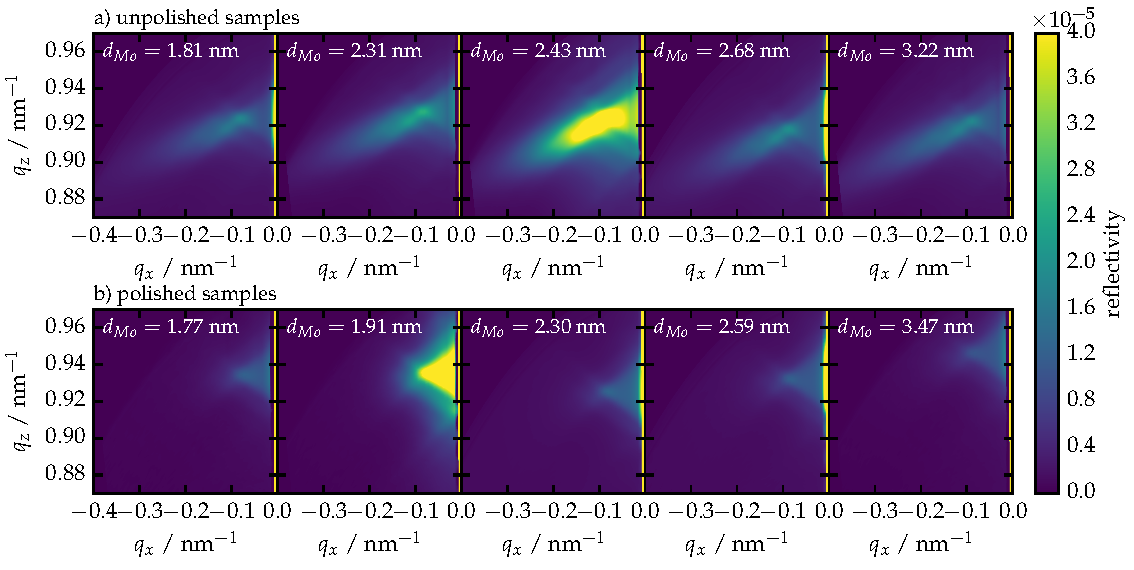
\includegraphics[width=\textwidth]{img/MoSiC_diffuse_measurements}
\caption{Measured diffuse scattering distributions in reciprocal space representation shown on linear false-color scale. The selected unpolished samples are shown in a) with increasing Mo layer thickness $d_{Mo}$. The selected samples for the polished set are shown in b) also in order of increasing Mo thickness $d_{Mo}$. The samples with strongest scattering are shown in larger detail in Fig.~\ref{fig:dwba_data_best_model_comparison}. The diffuse scattering was measured by keeping the detector angle with respect to the incoming beam fixed at $\Delta\Theta = 30^\circ$, while the sample was tilted from an AOI of $\alpha_i=15^\circ$ to $\alpha_i=38^\circ$ with a step size $\Delta\alpha_i = 0.5^\circ$. At each angular position, a wavelength scan from $\lambda=12.35$ nm to $\lambda=14.0$ nm in steps of $\Delta\lambda = 0.01$ nm was performed to map the diffuse scattering distribution.}
\label{ch_diff:fig_mo_si_c_diffuse}
\end{figure*}
The maps in Fig.~\ref{ch_diff:fig_mo_si_c_diffuse}a show the scattering distribution from the unpolished samples marked with the fitted Mo layer thickness as listed in table~\ref{ch_diff:tbl_mo_si_thickness_mcmc_result_selected_samples}. The polished samples are shown in Fig.~\ref{ch_diff:fig_mo_si_c_diffuse}b.

A very prominent observation in both sets, is that one sample in each series shows significantly stronger overall scattering than the others. In addition, both sets show distinctly different scattering distributions clearly differentiating the polished from the unpolished samples. In the case of the polished samples, significantly less scattering than for the unpolished ones can be observed for higher spatial frequencies $q_x$, whereas more intensity is measured for smaller frequencies. A recognizable characteristic of the off-specular scattering intensity is the observation of a downward tilted Bragg sheet in case of the unpolished samples, which is in contrast to the rocking scan map of the unpolished Mo/B$_4$C/Si/C sample from Sec.~\ref{ch_diff:sec_PTB17}. This is due to a non-orthogonal roughness correlation throughout the stack with respect to the surface and interfaces first observed by \textcite{gullikson_asymmetric_1999}. We have discussed the theoretical aspects of this effect in Sec.~\ref{ch_theo:sec_diffuse_scattering}, but shall investigate this behavior for the specific set of samples studied here.

The downward tilt of the Bragg sheet is clearly observed for all samples in the unpolished series with a similar direction. All samples were measured along the same nominal $x$ axis, i.e.~along the same direction with respect to their mounting orientation during the deposition process. Due to to in-plane measurement of the diffuse scattering, the non-orthogonal roughness correlation angle $\beta$ can only be evaluated along the projection of its directional vector onto the $x$-$z$-plane. However, the vertical correlation direction vector may not necessarily lie in that plane. To verify this property, we shall investigate the corresponding diffuse scattering distribution from the strongest scattering sample with $d_\text{Mo} = \nm{2.43}$ by rotating it by $\SI{90}{\degree}$ around its surface normal onto the sample holder and repeat the mapping of reciprocal space. Fig.~\ref{ch_diff:fig_diffuse_tilt_vs_notilt} shows the comparison of the map obtained earlier with the map from the rotated sample.
\begin{figure*}[htbp]
\centering
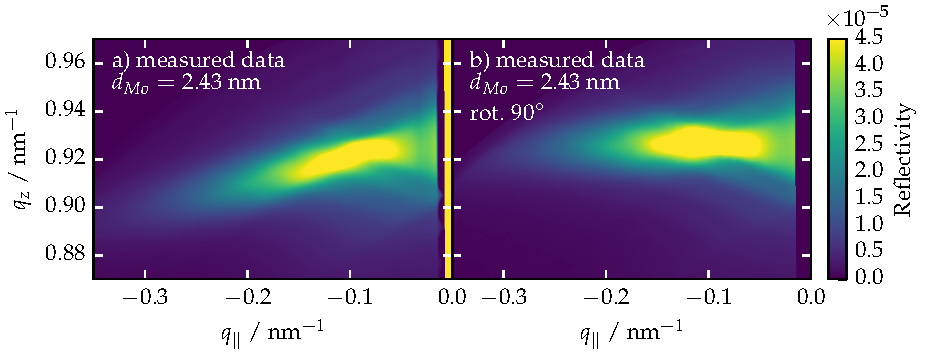
\includegraphics[width=\textwidth]{img/MoSiC_diffuse_tilt_vs_notilt}
\caption{a) Diffuse scattering map for the unpolished sample ($d=\nm{2.43}$) with strongest total scattering intensity measured at the same orientation as in Fig.~\ref{ch_diff:fig_mo_si_c_diffuse}. b) Corresponding reciprocal space map for the same sample but irradiated from a different angle by rotating the sample by $\SI{90}{\degree}$ around the surface normal. Clear differences in the tilt angle of the Bragg sheet can be observed associated with the vertical roughness correlation direction.}
\label{ch_diff:fig_diffuse_tilt_vs_notilt}
\end{figure*}
The tilt direction is clearly different for the map of the rotated sample, where we obtain a similarly horizontal Bragg sheet as for the Mo/B$_4$C/Si/C sample in Sec.~\ref{ch_diff:sec_PTB17}. Based on the evaluation of the tilt angle in both maps, it is possible to deduce the direction and total angle $\beta$ of the roughness correlation direction with respect to the surface normal and the orientation directions of the sample during the measurement. This angle is given by the two orthogonally measured Bragg sheet tilt angles $\beta^{\SI{0}{\degree}}$ and $\beta^{\SI{90}{\degree}}$ through
\begin{align}
 \tan^2(\beta) &= \tan^2(\beta^{\SI{0}{\degree}}) + \tan^2(\beta^{\SI{90}{\degree}}) \text{.} \label{ch_diff:eqn_total_beta}
\end{align}
These two independent measurements can be additionally used to verify the results of the reconstruction. We shall thus perform the analysis described in Sec.~\ref{ch_diff:sec_PTB17} and deduce the \gls{psd} parameters including the vertical correlation length as well as the non-orthogonal correlation direction for this sample in particular. For all other measured samples we proceeded in the same way, where here only the in-planar Bragg sheet tilt angle is determined.

\subsection{Reconstruction of the Interface Morphology}
The theoretical analysis was performed based on the method described in the first part of this chapter. Instead to applying the \gls{pso} method to reconstruct the parameters characterizing the interface morphology, the \gls{mcmc} procedure was applied to obtain the optimized parameter values and their confidence intervals. The basic principle is identical to that used in chapter~\ref{ch_spec} and relies on the minimization functional stated in Eq.~\eqref{ch_diff:eqn_chi_diffuse}, which enters the likelihood according to the definition in Eq.~\eqref{ch_spec:eqn_likelihood}. This method is computationally more challenging than applying only the \gls{pso} procedure, but becomes possible with the smaller number of periods ($N=50$) for the samples investigated here, since the effort scales with the order of $O(N^2)$. As starting values, the walkers for the \gls{mcmc} algorithm were distributed randomly across the parameter space given by the limits listed in table~\ref{ch_diff:tbl_PTB17_diffuse_optimization_limits_and_results} with the exception of the Hurst parameter. The latter is limited between $0.8$ and $1.0$, where the upper limit is the intrinsic theoretical limit representing Gaussian type roughness. The measurements conducted here only allow a limited access to the Hurst parameter, as it is determined by the asymptotic behavior of the \gls{psd} towards higher lateral roughness frequencies. For that spacial frequency range, however, no data exists as the vertical correlation of roughness is reduced and the detector threshold is reached so no asymptotic data can be recorded. Others \cite{rack_comparative_2010} have observed Hurst values in that range for similar samples with values close to the case of Gaussian roughness. The results for the Mo/B$_4$C/Si/C sample shown in Fig.~\ref{ch_diff:PTB17_PSD_for_all_geometries} are in good agreement with these findings resulting in a Hurst factor of $H=1.0$. There, an overall higher in-plane correlation length $\xi_\parallel$ compared to the unpolished samples here, allows a better determination of the asymptotic behavior of the \gls{psd}. Due to these results, we analyze the samples from both sets by fixing the Hurst parameter to $H=1.0$, i.e.~by applying a roughness model for Gaussian roughness only. However, in the determination of the confidence intervals, the range from $H=0.8$ to $H=1.0$ was considered to reflect this uncertainty in the determination of the parameters. 

The results of the ideal model for each sample system entering the DWBA calculation were obtained from the analysis in Sec.~\ref{ch_spec:sec_mo_si_c_results}. The optimization was conducted by applying the MCMC method with respect to the vertical correlation length $\xi_\perp$ in the vertical correlation function $c_\perp(q_\parallel)$, the tilt angle $\beta$ and all PSD parameters in $C(q_\parallel)$. For the two samples, the maps with the strongest scattering from each set are shown in comparison to the best model DWBA calculation found this way. 
\begin{figure*}[htbp]
\centering
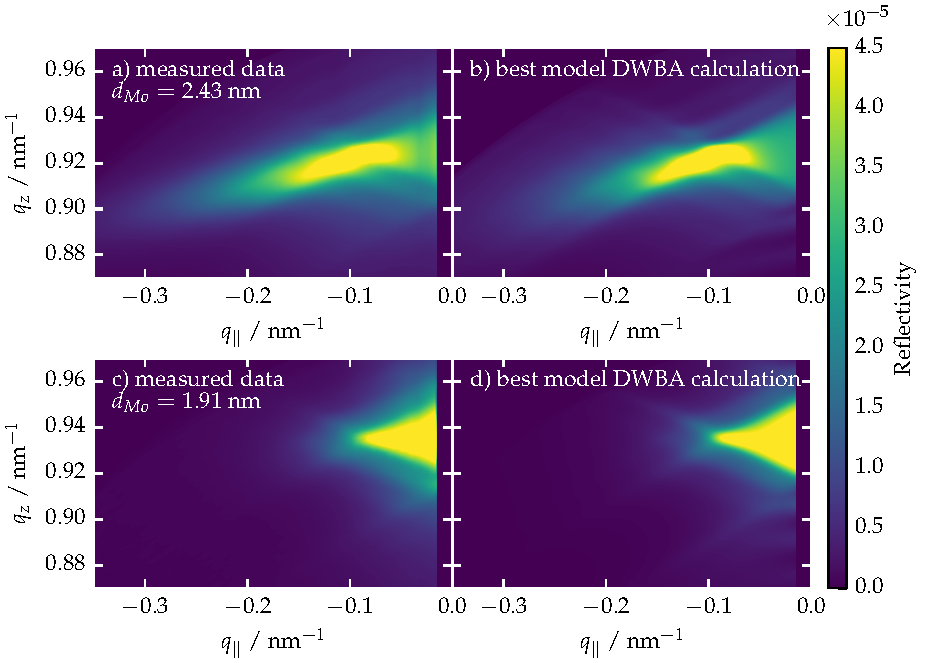
\includegraphics[width=\textwidth]{img/MoSiC_dwba_data_best_model_comparison}
\caption{Direct comparison of the measured reciprocal space maps with the DWBA calculation resulting from the parameters obtained with the MCMC optimization procedure (see text). a) shows the maps of the unpolished sample with strongest diffuse scattering. Similarly, b) shows the maps of the polished sample at the respective presumed crystallization threshold with strongest scattering.}
\label{fig:dwba_data_best_model_comparison}
\end{figure*}
The resulting maps in Fig.~\ref{fig:dwba_data_best_model_comparison} from the unpolished (a) and polished (c) samples show very good agreement with the theoretical calculations in (b) and (d), respectively, including the tilted Bragg sheet observed for the unpolished sample. All parameter values obtained from the \gls{mcmc} optimization procedure are compiled in Table~\ref{ch_diff:tbl_Mo_Si_C_diffuse_parameters_results}. 
\begin{table*}[htbp]
\centering
\caption{Results for the DWBA model parameters with the respective confidence intervals for both sample sets.}
\label{ch_diff:tbl_Mo_Si_C_diffuse_parameters_results}
\begin{tabular}{@{}lllll@{}}
\toprule
nom.~Mo thickness / nm&$\sigma_r$ / nm & $\xi_\parallel$ / nm & $\xi_\perp$  / nm$^{-1}$ & $\beta$ / $^\circ$ \\
(fitted Mo thickness / nm) & & & & \\ \midrule
\multicolumn{5}{c}{Unpolished samples}\\
\midrule
$1.70$ $(1.81[{-0.12}/{+0.24}])$ &$0.227^{+ 0.010}_{- 0.003}$ & $3.14^{+ 0.45}_{- 0.06}$ & $3.69^{+ 0.15}_{- 0.16}$ & $-4.62^{+ 0.05}_{- 0.06}$ \\ \addlinespace
$2.15$ $(2.31[{-0.22}/{+0.21}])$ & $0.232^{+ 0.009}_{- 0.002}$ & $3.72^{+ 0.44}_{- 0.05}$ & $4.88^{+ 0.17}_{- 0.18}$ & $-5.02^{+ 0.04}_{- 0.04}$ \\ \addlinespace
$2.30$ $(2.43[{-0.09}/{+0.16}])$& $0.329^{+ 0.009}_{- 0.003}$ & $4.51^{+ 0.45}_{- 0.06}$ & $4.44^{+ 0.17}_{- 0.17}$ & $-5.67^{+ 0.05}_{- 0.06}$ \\ \addlinespace
verification $90^\circ$ & $0.317^{+ 0.011}_{- 0.004}$ & $4.56^{+ 0.48}_{- 0.10}$ & $3.62^{+ 0.18}_{- 0.19}$ & $+0.55^{+ 0.07}_{- 0.07}$ \\ \addlinespace
$2.45$ $(2.68[{-0.13}/{+0.16}])$&  $0.211^{+ 0.009}_{- 0.003}$ & $3.61^{+ 0.46}_{- 0.06}$ & $3.80^{+ 0.15}_{- 0.16}$ & $-5.06^{+ 0.06}_{- 0.06}$ \\ \addlinespace
$2.90$ $(3.22[{-0.13}/{+0.11}])$& $0.243^{+ 0.009}_{- 0.002}$ & $2.89^{+ 0.43}_{- 0.03}$ & $5.72^{+ 0.14}_{- 0.17}$ & $-5.06^{+ 0.03}_{- 0.03}$ \\ \addlinespace
\midrule
\multicolumn{5}{c}{Polished samples}\\
\midrule
$1.70$ $(1.77[{-0.22}/{+0.19}])$ & $0.129^{+ 0.009}_{- 0.002}$ & $7.05^{+ 0.55}_{- 0.23}$ & $0.53^{+ 0.03}_{- 0.02}$ & $-1.19^{+ 0.28}_{- 0.28}$ \\ \addlinespace
$1.85$ $(1.91[{-0.12}/{+0.17}])$ & $0.195^{+ 0.008}_{- 0.002}$ & $10.66^{+ 0.56}_{- 0.19}$ & $0.76^{+ 0.04}_{- 0.04}$ & $-1.50^{+ 0.25}_{- 0.26}$ \\ \addlinespace
$2.00$ $(2.29[{-0.28}/{+0.13}])$& $0.105^{+ 0.005}_{- 0.001}$ & $8.95^{+ 0.52}_{- 0.13}$ & $0.76^{+ 0.03}_{- 0.03}$ & $-2.28^{+ 0.16}_{- 0.14}$ \\ \addlinespace
$2.30$ $(2.60[{-0.12}/{+0.14}])$& $0.106^{+ 0.006}_{- 0.001}$ & $8.22^{+ 0.52}_{- 0.17}$ & $0.86^{+ 0.04}_{- 0.04}$ & $-2.90^{+ 0.16}_{- 0.07}$ \\ \addlinespace
$3.05$ $(3.47[{-0.19}/{+0.13}])$& $0.088^{+ 0.005}_{- 0.001}$ & $10.29^{+ 0.58}_{- 0.19}$ & $1.47^{+ 0.13}_{- 0.11}$ & $-1.62^{+ 0.16}_{- 0.16}$ \\ \addlinespace
 \bottomrule
\end{tabular}
\end{table*}

The verification measurement of the rotated sample appears in the row below the respective sample and shows very good agreement with the original measurement. The only exception is the vertical correlation parameter $\xi_\perp$, which is lower in case of the rotated sample. This is due to a truncation of the scattering intensity to higher values of $|q_x|$, because of the absorption due to the Si L$_2$-edge. From the two measurements, a total non-orthogonal tilt angle of the vertical roughness correlation of $\beta = \SI{5.70\pm 0.06}{\degree}$ is obtained by applying Eq.~\eqref{ch_diff:eqn_total_beta}. This clearly indicates an anisotropy of the deposition process, which is likely due to non-central mounting of the sample on the sample holder during fabrication. For both sample sets, table~\ref{ch_diff:tbl_Mo_Si_C_diffuse_parameters_results} shows a significant increase of roughness $\sigma_r$ at the crystallization threshold at nominal molybdenum thicknesses of $d_\text{nom}=\nm{2.30}$ for the unpolished samples and $d_\text{nom}=\nm{1.85}$ for the polished samples. This coincides with the lowest reflectance for that sample in each set shown in Fig.~\ref{ch_spec:fig_EUV_peak_refl}. Interestingly, the roughness returns to the previous value for further increasing Mo layer thicknesses. This indicates, that the roughening due to the formation of nanocrystallites at the threshold is compensated for even larger thicknesses. We also observe a restored peak reflectance in Fig.~\ref{ch_spec:fig_EUV_peak_refl} in that case. For the polished samples, the formation of crystallites can be observed with similar effects, but at lower Mo layer thickness with overall significantly lower root mean square roughness $\sigma_r$. It should be noted, that the strong roughness increase is only observed from the diffuse scattering measurement in Fig.~\ref{ch_diff:fig_mo_si_c_diffuse} for one of the samples in each set in table~\ref{ch_diff:tbl_Mo_Si_C_diffuse_parameters_results}. This is despite the fact, that a reduced peak reflectance deviating from the expected theoretical values is seen for two samples out of each set in Fig.~\ref{ch_spec:fig_EUV_peak_refl}, that were associated with the crystallization threshold. In both cases, only the sample with the thicker molybdenum layer of the two shows stronger roughness, which we shall discuss in the following subsection. Another clear difference between the polished and unpolished sets prominently shown in table~\ref{ch_diff:tbl_Mo_Si_C_diffuse_parameters_results}, is the large gap between the vertical correlation factors $\xi_\perp$. In the unpolished case, values between $\xi_\perp=3.62(+ 0.18/- 0.19)$~nm$^{-1}$ and $\xi_\perp=5.72(+ 0.14/- 0.17)$~nm$^{-1}$ are found, whereas for the polished samples these values range between $\xi_\perp=0.53(+ 0.03/- 0.02)$~nm$^{-1}$ and $\xi_\perp=1.47(+ 0.13/- 0.11)$~nm$^{-1}$. As is to be expected, the polishing process largely reduces the roughness correlation between different interfaces as it alters the morphology of the interface. This situation corresponds to the low vertical roughness correlation illustrated in the left part of Fig.~\ref{ch_theo:fig_vertical_roughness_correlation}. In the case of unpolished growth, almost the entire stack is correlated (see the right part of Fig.~\ref{ch_theo:fig_vertical_roughness_correlation}) for the observable spatial frequencies. The large values for the in-planar correlation length $\xi_\parallel$ for the polished samples (between $\xi_\parallel = 7.05(+0.55/-0.23)$~nm and $\xi_\parallel = 10.66(+0.56/-0.19)$~nm) are also a direct result of the polishing process as high spacial frequencies $q_x$ are successfully reduced due to the smoothing of the polishing process.

\subsection{Discussion of the Results}
Finally, we shall interpret the results and relate them to the findings made in Sec.~\ref{ch_spec:sec_mo_si_c}. To illustrate the relation between the peak reflectance (originally shown in Fig.~\ref{ch_spec:fig_EUV_peak_refl}) of each sample and the \gls{rms} roughness reconstructed here, Fig.~\ref{ch_diff:fig_Mo_Si_C_PSD_results} shows these parameters in comparison with each other. In addition, the N\'{e}vot-Croce parameter from the specular reflectance analysis performed in Sec.~\ref{ch_spec:sec_mo_si_c_results} is included through its confidence interval to allow the distinction of intermixing and roughness.
\begin{figure*}[htbp]
\centering
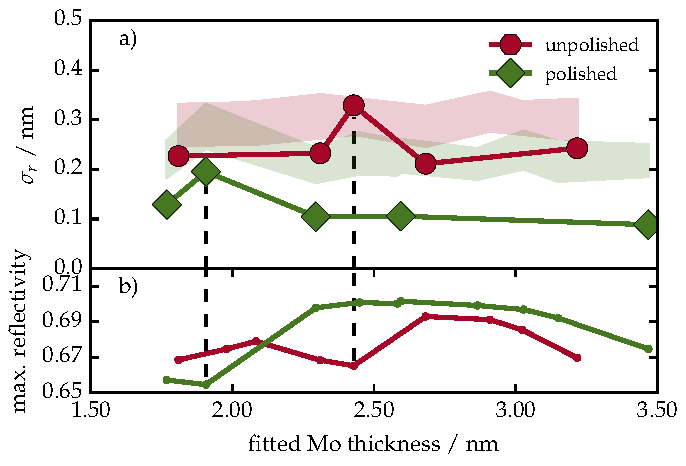
\includegraphics[width=0.75\textwidth]{img/MoSiC_PSD_results}
\caption{a) Root mean square roughness results from the analysis of the diffuse scattering for the two sample sets together with the full confidence intervals of the N\'{e}vot-Croce damping factor as obtained from the structural analysis in Sec.~\ref{ch_spec:sec_mo_si_c}. In each set, an increase of roughness is observed at the crystallization threshold. For comparison, the max peak reflectance for each sample set is shown in b). The increase in roughness clearly correlates with a significant dip in the peak reflectance as indicated by the dashed vertical lines.}
\label{ch_diff:fig_Mo_Si_C_PSD_results}
\end{figure*}

The reconstructed roughness values shown in the figure have the expected increase at the presumed crystallization threshold for each set. In Fig.~\ref{ch_spec:fig_MoSi_fitted_mo_and_fitted_D}(b), a simultaneous jump in the total period thickness $D$ at this threshold for both sample sets was observed at the molybdenum layer thickness around $d_\text{Mo} = 2.5$ nm for the unpolished samples and $d_\text{Mo} = 2.2$ nm for the polished samples. The evaluation of the diffuse scatter revealed increased roughness throughout the multilayer stack for the samples just at the thickness jump. In comparison to the suspected trend of the peak reflectance with $d_\text{Mo}$ in Fig.~\ref{ch_spec:fig_EUV_peak_refl} two samples with lower reflectance in both sets were observed, one exactly at the position of this increased scatter at $d_\text{Mo}=2.43(+0.16/-0.09)$~nm for the unpolished samples and $d_\text{Mo}=1.91(+0.17/-0.12)$~nm for the polished samples, and the other sample with nominally $0.15$ nm lower thickness at $d_\text{Mo}=2.31(+0.21/-0.22)$~nm for the unpolished samples and $d_\text{Mo}=1.77(+0.19/-0.22)$~nm for the polished samples, respectively. At least for the unpolished samples, this higher roughness $\sigma_r$ at $d_\text{Mo}=2.43(+0.16/-0.09)$~nm is not observed from evaluating the specular reflectance alone, where the reflectance is diminished by the combined effects of roughness, intermixing and compound formation, which is represented by an effective $\sigma$-value in the N\'{e}vot-Croce factor. In contrast, for the polished samples the enhanced scatter is also observed in the total N\'{e}vot-Croce damping factor as indicated by the confidence interval in Fig.~\ref{ch_diff:fig_Mo_Si_C_PSD_results} at $d_\text{Mo}=1.91(+0.17/-0.12)$~nm. In the polished system, the magnitude of the peak reflectance decrease visible as the difference between theoretical expectation and actually measured value in Fig.~\ref{ch_spec:fig_EUV_peak_refl}, however, is also significantly higher for the two respective samples, compared to the rest of the set, than for the unpolished samples. This may explain that an increase in the damping factor is less pronounced. The roughness amplitudes $\sigma_r$, as derived from the diffuse scatter, however, have much smaller values than the N\'{e}vot-Croce factor $\sigma$. The comparison of the N\'{e}vot-Croce parameters and the roughness values reveals, that the polishing successfully reduced the roughness contribution to the overall damping factor. It should be noted, that the N\'{e}vot-Croce parameters confidence intervals have reduced less than the roughness $\sigma_r$, compared to the series of unpolished samples. This shows, that the remaining interface distortions through compound formation and intermixing are largely responsible for the gap between theoretically possible maximum reflectance and actual measured values for the polished set.

The interpretation of these findings is in line with the observation of the formation of crystallites in the molybdenum layer at around $2$ nm thickness reported by \textcite{bajt_investigation_2001}. Particularly, the threshold is assigned to the lower thickness where the reflectance first decreases (at $d_\text{Mo}=2.31(+0.21/-0.22)$~nm for the unpolished set and at $d_\text{Mo}=1.77(+0.19/-0.22)$ for the polished set) without an observation of increased roughness by diffuse scatter. This is explained by the crystallization process starting with increased intermixing and small seeds corresponding to a short correlation length. This yields a high spacial frequency roughness, which is not correlated throughout the stack. The corresponding scatter is, thus, not resonantly enhanced. Without the enhancement, it is below the detection threshold of the diffuse scattering experiment conducted here. With increasing crystallites, the diffuse scatter becomes observable at slightly higher molybdenum thickness. Note that for the unpolished sample, the threshold coincides with the point where the ideal Mo-to-Si ratio should yield the highest reflectance in agreement with the findings in \cite{bajt_investigation_2001} and the theoretical calculations shown in Fig.~\ref{ch_spec:fig_EUV_peak_refl}. For the polished samples, this threshold is shifted to thinner molybdenum layers around $d_\text{Mo} = 1.77(-0.22/+0.19)$ nm. This is beneficial for the peak reflectance, which is higher at the optimum ratio, than for the unpolished set. In both cases, a smoothing occurs for even larger molybdenum thickness, restoring the roughness to its value below the threshold. The evaluation of the diffuse scatter shows an overall lower roughness for the polished samples than for the unpolished ones and, particularly, a destruction of vertical roughness correlation $\xi_\perp$ throughout the stack shown in table~\ref{ch_diff:tbl_Mo_Si_C_diffuse_parameters_results} and an increase of the in-planar correlation length $\xi_\parallel$ (describing a reduction of high-spacial frequency roughness), as intended by the polishing. 

Finally, we note that the based on the analysis methods introduced in Sec.~\ref{ch_spec:sec_mo_si_c} and the diffuse scatter analysis explained in beginning of this chapter is is possible to consistently determine the molybdenum layer thickness and the average power spectral density roughness for the interfaces throughout the full multilayer stack. The application of these methods to Mo/Si multilayer samples with varying molybdenum thickness with/without polishing confirmed previous findings on the onset of molybdenum crystallization in the literature. The results presented in Sec.~\ref{ch_spec:sec_mo_si_c} and the analysis of the diffuse scatter discussed here are published together in \fullcite{haase_interface_2017}.

\section{Roughness and Intermixing in Cr/Sc Multilayers} \label{ch_diff:sec_CrSc}
In Sec.~\ref{ch_spec:sec_CrSc}, we have demonstrated the analysis of Cr/Sc multilayer mirrors with sub-nanometer layer thicknesses. A more complex model was required to reconstruct the structural parameters unambiguously. The combination of several experiments conducted, could indeed provide a unequivocal solution to most of the parameters shown in table~\ref{ch_spec:tbl_CrSc_gradual_parametrization}, with the results and their confidence intervals listed in table~\ref{ch_spec:tbl_CrSc_MCMC_results} and illustrated in Fig.~\ref{ch_spec:fig_CrSc_confidence_intervals}. However, as for the Mo/Si systems investigated in this thesis, the methods applied in Ch~\ref{ch_spec} do not yield a possibility to distinguish roughness from intermixing. Even though, the spatially resolved methods such as \gls{xrf} did in combination yield the interface profile asymmetry, a correlation between the intermixing parameter $\eta$ and the \gls{rms} roughness parameter $\sigma_r$ remains, as seen in Fig.~\ref{ch_diff:fig_eta_sigma_correlation}.
\begin{figure}[htbp]
  \centering
  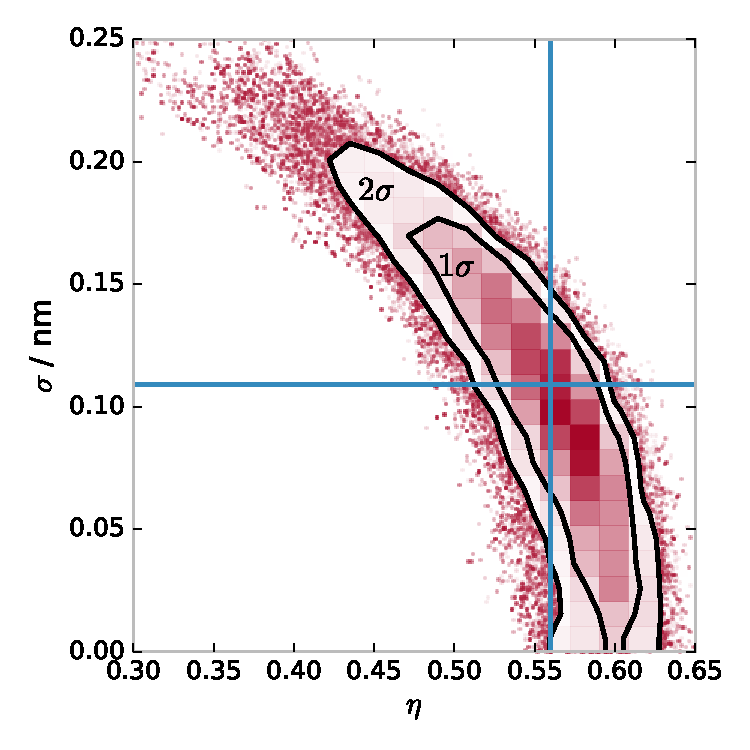
\includegraphics[width=0.5\textwidth]{images/eta_sigma_correlation}
  \caption{Correlation of the projected $\chi^2$ surface onto the parameter 
pair $(\eta, \sigma_r$) by visualization of the position of the MCMC samples in 
the reduced parameter space.}
  \label{ch_diff:fig_eta_sigma_correlation}
\end{figure}

Based on the analysis of the diffuse scatter, as we have shown above, that distinction becomes possible. We finalize this chapter with the analysis of the Cr/Sc sample system studied in Sec.~\ref{ch_spec:sec_CrSc} and complete the characterization with respect to that parameter correlation. For that purpose, we have measured the diffuse scattering intensity from the Cr/Sc sample similarly to the Mo/Si sample systems above in a rocking scan geometry. As the theoretical model for the \gls{dwba} calculation, we applied the gradual interface model as defined in the previous chapter with the optimal parameters listed in table~\ref{ch_spec:tbl_CrSc_MCMC_results} for the combination of all analytic experiments conducted there.

The reciprocal space map was taken at an opening angle of $\Delta \Theta = \SI{3}{\degree}$, where the specular reflectance condition corresponds to the situation where the \gls{euv} reflectivity was evaluated in the previous chapter. This is necessary for this particular sample system to fulfill the Bragg condition without decreasing the wavelength to values below the Sc L-edge, where absorption would eliminate the possibility to diffuse scattering from the multilayer. The measurement results are shown in Fig.~\ref{ch_diff:fig_CrSc_diffuse_meas}.
\begin{figure}[htbp]
  \centering
  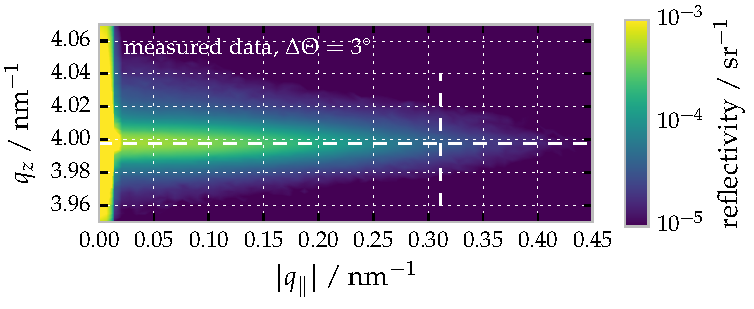
\includegraphics[width=0.7\textwidth]{img/CrSc_diffuse_measured}
  \caption{Diffuse scattering measurement in $q$-space representation and 
log scale.}
  \label{ch_diff:fig_CrSc_diffuse_meas}
\end{figure}
A clear difference to the maps in case of Mo/Si samples is the lack of Kiessig-like peaks and a similar triangular shaped intensity distribution due to the Bragg-like peak. Here, rather the expectation issued at the beginning of the chapter of the observation of a well formed Bragg sheet is met. The reasons behind this different behavior are the fundamental differences with respect to the quality as a mirror of the Cr/Sc system compared to the Mo/Si system and the different measurement geometry. With a \gls{euv} peak reflectance of only about $\SI{15}{\percent}$, only approximately $\SI{27}{\percent}$ of the maximum theoretical reflectivity is attained. In the previous chapter, it was found that the gradually shaped interfaces regions and intermixing of the sub-nanometer thick layers play a fundamental role in diminishing the reflectivity. This, however, does also crucially reduce the impact of multiple dynamic reflections, which were found to have a strong impact on the measured diffuse scatter intensity for the Mo/Si multilayer systems investigated above. In addition, this causes significantly higher penetration depth allowing more layers to contribute to the diffuse scatter, even if the Bragg condition is fulfilled for both the incidence and exit angles. Apart from the general lack of dynamic effects due to bad reflectivity at the interfaces, the non-appearance of Kiessig-like peaks is also related to the rocking scan geometry with a significantly smaller opening angle. In the comparison of geometries done at the beginning of this chapter in Fig.~\ref{ch_diff:fig_kiessig_like_peaks_diffuse_map}, we have shown that the resonance conditions move to higher absolute values of $q_\parallel$, if the opening angle is reduced. Thus, no peaks are to be expected in the accessible range for the scan geometry chosen here.

\subsection{Estimation of the Vertical Roughness Correlation and the PSD}
The sample investigated here is represented by the gradual interface model introduced in Sec.~\ref{ch_spec:sec_mo_si_c} above. With total number of $N=400$ bilayers and subsequent subdivision in sublayers, a substantial increase of interfaces has to be considered for the \gls{dwba} analysis as compared to the Mo/Si systems. As pointed out above, the computation cost growth quadratically with the order $O(N^2)$ and thus renders the \gls{mcmc} method very unpractical for this particular system. However, in order to deduct an estimate of the \gls{psd} and the vertical roughness correlation, we shall apply the approach introduced in Sec.~\ref{ch_diff:sec_PTB17} at the beginning of the chapter by analyzing only selected cuts of the map to obtain the relevant parameters. The best \gls{psd} model parameters are then obtained by analyzing a horizontal cut of the Bragg sheet divided by the multilayer enhancement factor. The two cut positions are shown in Fig.~\ref{ch_diff:fig_CrSc_diffuse_measured_vs_dwba} as dashed lines in both, the measured maps and the best model \gls{dwba} calculation that was obtained with this approach.
\begin{figure}[htbp]
  \centering
  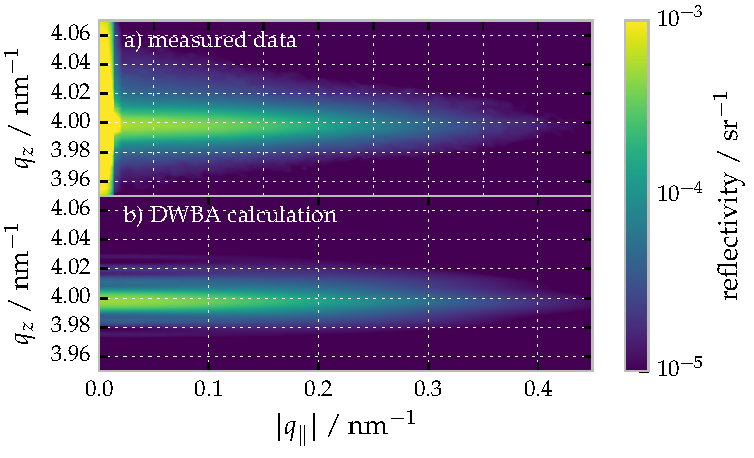
\includegraphics[width=0.7\textwidth]{img/CrSc_diffuse_measured_vs_dwba}
  \caption{a) Diffuse scattering measurement in $q$-space representation and 
log scale. b) DWBA calculation of the optimal PSD model based on the gradual interface model with the multilayer parameters for the combined analysis listed 
in Table~\ref{ch_spec:tbl_CrSc_MCMC_results}.}
  \label{ch_diff:fig_CrSc_diffuse_measured_vs_dwba}
\end{figure}
The comparison shows a good agreement of the model with the measured data. The data and the simulation results at the vertical cut position are shown in detail in Fig.~\ref{ch_diff:fig_CrSc_diffuse_vertical_correlation}.
\begin{figure}[htbp]
  \centering
  \includegraphics[width=0.7\textwidth]{img/CrSc_diffuse_vertical_correlation}
  \caption{Measured data and calculations at the vertical cut indicated by the vertical white dashed line in Fig.~\ref{ch_diff:fig_CrSc_diffuse_measured_vs_dwba}. The blue dashed lines show two limiting cases for the value of the vertical correlation length. The result is a model uncertainty in the PSD.}
  \label{ch_diff:fig_CrSc_diffuse_vertical_correlation}
\end{figure}
The solid red line represents the measured data extracted at the aforementioned vertical cut position. The best model result was obtained using the \gls{pso} algorithm and is shown as solid blue line providing a good match with the data. The measurement uncertainty is indicated through the red shaded area. Due to the very high computational cost of the MCMC procedure mentioned above, we have instead
calculated two limiting cases of the vertical correlation to assess the confidence interval for that parameter. The results of that calculation are shown as dashed blue lines framing the measurement uncertainty at the position of the peak. This parameter enters the calculation of the multilayer enhancement factor marked in Eq.~\eqref{ch_diff:eqn_full_explicit_dwba_with_approximations} and thus affects the absolute values of the \gls{psd} extracted from the horizontal cut by dividing through that term. It thus introduces a numerical or model uncertainty to the deduction of the \gls{psd}. Proceeding from here, we have evaluated the measured 
\gls{psd}. To deduct the effective power spectral density, we have taken the cut along the Bragg sheet as indicated by the horizontal white dashed lines in the reciprocal space 
maps. We divided the extracted scattering intensity by the multilayer 
enhancement factor, leaving the contribution of the effective \gls{psd} $C(q_\parallel)$ to the diffuse scattering. Again, the two limiting cases are shown as red dashed curves in 
Fig.~\ref{ch_diff:fig_CrSc_diffuse_PSD} including the \gls{psd} deduced from the best model 
value for $\xi_\perp$ as a solid red curve.
\begin{figure}[htbp]
  \centering
  \includegraphics[width=0.7\textwidth]{img/CrSc_diffuse_PSD}
  \caption{Comparison of the extracted effective PSDs from the diffuse 
scattering measurement. The 
uncertainty interval for the extracted power spectral density is shown by the 
two dashed PSD profiles (see main text).}
  \label{ch_diff:fig_CrSc_diffuse_PSD}
\end{figure}
The \gls{rms} roughness, which we seek to determine to solve the correlation problem illustrated in Fig.~\ref{ch_diff:fig_eta_sigma_correlation} above, is given by the two-dimensional integral of the \gls{psd} as
\begin{align}
\sigma_r &=\frac{1}{2\pi} \sqrt{\int_{0}^{\infty} q_\parallel C(q_\parallel) \, 
dq_\parallel} \text{.}
\end{align}
The uncertainty of the \gls{psd} due to the vertical correlation leads to an 
uncertainty in the \gls{rms} roughness when evaluating the integral. Due to the 
limited $q_\parallel$ range where measurements can be taken, we have fitted the 
\gls{psd} model of Eq.~\eqref{ch_theo:eqn_psd} to the resulting data by applying the \gls{pso} method based on the parameter limits shown in table~\ref{ch_diff:tbl_PTB17_diffuse_optimization_limits_and_results}. The additional uncertainty introduced through the model estimate causes a systematic error of the \gls{psd} extraction and confidence intervals for the parameters were determined by separately fitting the resulting alternative \gls{psd}s. The tilt angle beta was fixed to $\beta=\SI{0}{\degree}$ in this analysis, since no non-orthogonal roughness correlation was determined by comparison of vertical cuts at different $q_\parallel$ positions in the map at this sample orientation. After that, the integration over the full $q_\parallel$ range was performed for the best model. The deviation of the integration for the \gls{psd} model fit and the data in the available range were negligible. The best model results for the vertical replication factor and the power spectral 
density are given in Table.~\ref{ch_diff:tbl_CrSc_psd_results}, together with their estimated
uncertainties.
\begin{table}
\centering
\caption{Best model parameters and confidence intervals of the \gls{psd} as a result of the diffuse scattering analysis for the gradual Cr/Sc system.}
\label{ch_diff:tbl_CrSc_psd_results}
\begin{tabular}{@{}lll@{}}
\toprule
Parameter & Best model values & Confidence interval\\ \midrule
$\sigma_r$ / nm & $0.17  $&$(-0.01/+0.02)$ \\
$\xi_\parallel$ / nm& $3.93 $&$(-0.42 / +0.33)$ \\
$\xi_\perp$  / nm$^{-1}$& $10.5 $&$ (-3.5/+3.5)$ \\
$H$ & $1.0$ & $(-0.03 /+0.0)$ \\
$\beta$ / $^\circ$ & $0.0$ & - \\
 \bottomrule
\end{tabular}
\end{table}

\subsection{Results and Conclusions}
In Sec.~\ref{ch_spec:sec_CrSc}, we have demonstrated a robust method to characterize ultra-thin 
multilayer systems with subnanometer layer thicknesses unambiguously. Layer 
thicknesses in the subnanometer region are necessary for near-normal incidence 
reflective mirrors in the water window spectral range. However, they come with 
the cost of increasing susceptibility to disturbances in the interfaces at the 
layer boundaries. This limits the achievable reflectance to values well below 
the theoretical threshold. The main mechanisms for diminished reflectance are 
interdiffusion and roughness. With these effects ranging on the order of the 
layer thickness, models based on binary layer stacks become inadequate to 
describe the physical situation. In order to find a proper representation of 
the multilayer sample, more sophisticated models with an explicit description 
of the gradual interdiffusion layers become necessary. This inevitably 
increases the number of parameters to be determined in analytical experiments. 
Finding an unambiguous solution is challenging and can only be achieved with a 
combined analysis of several non-destructive techniques.

We performed a rigorous analysis of several experimental methods to determine 
the model parameters representing one Cr/Sc sample. The optimal set of 
parameters was determined by applying a particle swarm optimizer in conjunction 
with a Markov-chain Monte Carlo method to verify the uniqueness of the solution 
and derive confidence intervals for all parameters in all experiments. Within the verified confidence intervals the \gls{mcmc} method reveals a remaining 
correlation between the intermixing parameter $\eta$ and the roughness factor $\sigma_r$, which 
could not be resolved with the experiments in specular geometry and the fluorescence measurements. In this chapter, we therefore 
performed a measurement of the off-specular diffuse scattering to distinguish 
between the roughness and the interdiffusion similarly to the approach used for the Mo/Si systems. The \gls{rms} roughness value found with the analysis of the diffuse scattering is identical within its confidence interval to the value obtained from the combined analysis and thus confirms the intermixing and roughness parameters listed in Table.~\ref{ch_spec:tbl_CrSc_MCMC_results}. The results of this analysis further reveal a high degree of roughness correlation throughout the multilayer, which is in agreement with observations made for the unpolished Mo/Si systems and hints at a strong roughness replication during deposition of each layer. It should also be noted here that the interdiffusion width 
$s_d$ is much larger than the roughness values $\sigma_r$. Also none of the 
layers was found to have the index of refraction of pure Cr or Sc, 
respectively. This is reflected through the non-vanishing intermixing parameter 
$\eta>0$. Thus, it can be concluded that while roughness still exists, 
Intermixing and interdiffusion of the two materials in these sub-nanometer layer systems are the main cause of diminished reflectance for the Cr/Sc multilayer system studied here.

The findings made in Sec.~\ref{ch_spec:sec_CrSc} together with the diffuse scattering analysis presented here have been published in \fullcite{haase_multiparameter_2016}.
%     \chapter{Summary and Outlook} \label{ch_summary}
This thesis is dedicated to the characterization of multilayer mirrors systems by means of the combination of several indirect methods based on reflection, fluorescence and scattering using \gls{euv} and X-ray radiation. The systems investigated in this framework belong to two very important applications using wavelengths within the \gls{euv} range. With the semiconductor industry moving towards next-generation lithography systems employing radiation at \nm{13.5}, multilayer mirrors made from Mo/Si layers with the addition of different barrier layers were characterized with respect to their structure and interface morphology. The second system of interest in the presented study are suitable to reflect radiation in the water window spectral range. More specifically, for radiation close to the Sc L-edge at approximately \nm{3.1}. For that purpose, \gls{euv} reflectivity, \gls{xrr}, \gls{reuv} and \gls{xrf} have been applied as methods to determine the layer structure.

It has been demonstrated that the problem of uniqueness and accuracy associated with the structural reconstruction of such systems is of high relevance to deduct reliable reconstructions.

    \printbibliography[heading=bibintoc,title={References}]

% 
\backmatter
    \pagestyle{thesisINTRO}
    %\pagestyle{empty}
\selectlanguage{ngerman}
\noindent
\section*{Acknowledgement}
At this point, I would like to express my gratitude to all of those who directly or indirectly contributed to the successful completion of this thesis.

First and foremost, I would like to thank Dr.~Frank Scholze, head of the EUV radiometry group at the Physikalisch-Technische Bundesanstalt, for giving me the chance to conduct the work leading to this PhD thesis under his supervision. Our numerous scientific discussions, his valuable ideas and his constructive criticism bundled with the opportunity to conduct experiments even on a short notice, contributed significantly to the success of this thesis.

Furthermore, I would like to thank Prof.~Dr.~Mathias Richter for his support and the examination of this thesis. He always had an open ear and valuable advise for the course of my scientific work and the near future. 

I am very grateful to Prof.~Dr.~Stefan Eisebitt for supporting and evaluating my dissertation and to Dr.~Sa\v{s}a Bajt for the fruitful discussions and collaboration, for providing me with the Cr/Sc samples for my experiments and her willingness to serve as evaluator of this thesis. In addition, I thank Dr.~Stefan Braun for contributing the Mo/Si multilayer mirror samples.

I also like to acknowledge all of my current and former colleagues and fellow graduate students, first of all my mentor, Dr.~Victor Soltwisch, who supported me during the past years. I would also like to thank Anal\'{i}a Fern\'{a}ndez Herrero, Raül Garc\'{i}a Diez, Dr.~Christian Gollwitzer, Dr.~Philipp Hönicke, Mika Pflüger and Dr.~Jan Wernecke. Our many intense discussions and the collaborative atmosphere they helped to establish improved my research significantly.

I am sincerely grateful to all members of the working group 7.12, Christian Buchholz, Ayhan Babalik, Anja Babuschkin, Martin Biel, Benjamin Dubrau, Andreas Fischer, Anne Hesse, Sina Jaroslawzew, Florian Knorr, Dr.~Christian Laubis, Jana Lehnert, Heiko Mentzel, Jana Puls, Anja Schönstedt, Christian Stadelhoff. Without their support and patience in many late-night beamtimes in the laboratory, this work would not have been possible. My honest thanks also go to all other colleagues of the PTB in Berlin-Adlershof.

Finally, I am in dept to all of my friends and family for their endless support and their distractions during my studies and over the course of my PhD thesis. Most importantly I would like to name Michl, Michael, Paul, Laura, Tim, Anna, Leo and my parents Detlev and Martina. Last but not least, I am deeply grateful to my grandfather Dr.~Walther Neudert for inspiring me and his early encouragement of my scientific career.








\cleardoublepage

    %\selectlanguage{ngerman}

\section*{Eidesstattliche Versicherung}
\vspace{3ex}

Hiermit versichere ich an Eides statt, dass ich die vorliegende Arbeit selbstständig verfasst und keine anderen als die in der Dissertation angegebenen Quellen und Hilfsmittel benutzt habe.
Alle Ausführungen, die anderen veröffentlichten oder nicht veröffentlichten Schriften wörtlich oder sinngemäß entnommen wurden, habe ich kenntlich gemacht.
Die Darstellung des Eigenanteils an bereits publizierten Inhalten in meiner beigefügten Erklärung ist zutreffend.
\vspace{3cm}

\noindent Berlin, den \today \hfill Anton Haase

\cleardoublepage

    %% publication list
\noindent
\pagestyle{empty}
\selectlanguage{ngerman}

\section*{Erklärung}

Es wurden bereits Teile der Dissertation veröffentlicht.
\vspace{2ex}

Liste der Veröffentlichungen, welche in die Dissertation eingeflossen sind:

\begin{enumerate}[label=\arabic*) ]
    \item \fullcite{haase_role_2014} 

    \item \fullcite{haase_characterization_2015} 

    \item \fullcite{haase_multiparameter_2016} 

    \item \fullcite{haase_interface_2017} 

\end{enumerate}
Liste der Veröffentlichungen, welche nicht in die Dissertation eingeflossen sind:
\begin{enumerate}[label=\arabic*) ]
    \item \fullcite{prasciolu_extended_2015} 

    \item \fullcite{soltwisch_correlated_2016} 
    
\end{enumerate}


Ich habe an keiner anderen Hochschule oder Fakultät eine Promotionsabsicht eingereicht.

\vspace{3cm}

\noindent Berlin, den \today \hfill Anton Haase

\cleardoublepage

    
\iffalse
    \bibliography{zotero-full.bib}
\fi

\end{document}
